\documentclass[a4paper,12pt,oneside]{book}
\linespread{1.5}
\usepackage{geometry}
\geometry{top=2cm,bottom=2.5cm,left=3.5cm,right=3.5cm} % Impostiamo il valore dei margini.
\usepackage[utf8]{inputenc}
\usepackage{tikz,pgf}
\usepackage{amsfonts}
\usepackage[italian]{babel} %% Abbiamo istruito LaTeX ad usare la lingua italiana.
\usepackage{todonotes}
\usepackage{subfig}
\usepackage{fancyhdr}
\setlength{\parindent}{0cm}

\usepackage{graphicx}
\usepackage{float}
\usepackage{csquotes}
\usepackage{amsmath}
\usepackage{numprint}
\usepackage{pgfplots}
\usepackage{pgfplotstable}
\usepackage{tocbibind}
\setcounter{tocdepth}{3}
\usepackage[hidelinks]{hyperref}
\usepackage{eurosym}

\usepackage{fancyhdr}
\pagestyle{fancy}
\renewcommand{\headrulewidth}{0pt}
\fancyhf{}
\fancyhead[L]{}
\fancyfoot[C]{\thepage}

\graphicspath{{imgs/}} %% cartella dalla quale ricavare le immagini %%

\setlength {\marginparwidth }{2cm} 
\pgfplotsset{compat=1.16}

\newenvironment{dedication}
  {\clearpage           % we want a new page
   \thispagestyle{empty}% no header and footer
   \vspace*{\stretch{1}}% some space at the top 
   \itshape             % the text is in italics
   \raggedleft          % flush to the right margin
  }
   {\par % end the paragraph
   \vspace{\stretch{3}} % space at bottom is three times that at the top
   \clearpage           % finish off the page
  }
  
\begin{document}
%% Frontespizio %%
\begin{titlepage}
    \begin{center}
    \vspace*{0.2cm}
    \begin{figure}[H]
        \centering
        
\includegraphics[width=0.8\textwidth]{imgs/logo.png}
    \end{figure}
        \vspace{5mm}
%% Dipartimento %%
    	\uppercase{\normalsize Dipartimento di Ingegneria Informatica, Modellistica, Elettronica e Sistemistica}\\
    \end{center}
    \begin{center}
%% Corso di Laurea %%
    	\large{ Corso di Laurea Ingegneria Informatica \\ Cybersecurity}\\
        \vspace{3mm}
        %%\large{\bf Progetto Sistemi Informativi }\\
    	\vspace{10mm}
%% Titolo della Tesi %%
    {\LARGE{\bf Tuning Ledger: Piattaforma Blockchain per la Certificazione del Tuning Automobilistico }}\\	
     \vspace{7mm}
    \end{center}
    
    \vspace{25mm}
    \noindent
    \begin{minipage}[t]{0.47\textwidth}
%% Relatore %%
    	{\large{ \bf Prof. \\Domenico Saccà}}
    	\vspace{12mm}
    \end{minipage}
    \hfill
    \begin{minipage}[t]{0.4\textwidth}\raggedleft
%% Candidato %%
    	{\large{\bf Gabriele Hamil\\ Mat. 256747 \\ \bf Matteo Stricagnolo \\ Mat. 252309}}
    \end{minipage}
    
    \vspace{30mm}
    
%% Anno Accademico %%
    \centering{\large \uppercase{ Anno Accademico 25/26}}

\end{titlepage}

%% Corpo della tesi %%

%%\chapter*{Sommario} %% In questa zona inseriamo l'abstract del nostro documento. %%
%%Inserisci abstract: ...


\tableofcontents
\listoffigures
\chapter{Sommario e Introduzione}

\section{Descrizione dell'Idea Progettuale}

L'obiettivo del progetto è realizzare Tuning Ledger, una piattaforma basata su tecnologia blockchain per la registrazione, la certificazione e la consultazione delle modifiche apportate a un veicolo dopo l'immatricolazione, garantendo trasparenza, autenticità e verificabilità delle informazioni lungo l'intero ciclo di vita del mezzo.

\subsection*{Criticit\`a}

Il settore della personalizzazione dei veicoli --- interventi sulla meccanica, sull'assetto, sull'impianto frenante o sull'estetica --- ha assunto negli ultimi anni una rilevanza economica crescente, alla quale non ha per\`o corrisposto un'evoluzione degli strumenti di documentazione. Le modifiche continuano a essere attestate attraverso fatture, dichiarazioni di conformit\`a e annotazioni sul libretto di circolazione: strumenti eterogenei, prodotti da soggetti diversi, facilmente smarribili e privi di qualunque garanzia di integrit\`a nel tempo.

Da questa frammentazione documentale discendono criticit\`a che investono l'intera filiera:

\begin{enumerate}
    \item \textbf{Asimmetria informativa}: al momento della rivendita l'acquirente non dispone di alcuno strumento indipendente per accertare quali lavorazioni siano state realmente eseguite, da chi, con quali componenti e nel rispetto di quali requisiti di omologazione.
    \item \textbf{Vulnerabilit\`a della documentazione}: certificati e schede tecniche in formato cartaceo o digitale non protetto sono esposti ad alterazione e falsificazione, senza che alcun meccanismo impedisca tecnicamente la retrodatazione di un intervento.
    \item \textbf{Rischio legale e onere di verifica}: la Concessionaria assume un rischio nel commercializzare un veicolo modificato di cui non pu\`o dimostrare la piena conformit\`a, mentre il Centro di Certificazione \`e costretto a ricostruire manualmente la storia degli interventi prima di poter procedere al collaudo.
    \item \textbf{Perdita di valore del mezzo}: chi ha investito in personalizzazioni eseguite a regola d'arte non \`e in grado di dimostrarne la qualit\`a e la regolarit\`a, e l'incertezza si traduce in una svalutazione sul mercato dell'usato.
\end{enumerate}

\subsection*{Tecnologia e funzionalit\`a}

La risposta a tali criticit\`a \`e il \textbf{Digital Modified Vehicle Passport} (DMVP): un passaporto digitale immutabile, associato univocamente al numero di telaio, che accompagna il veicolo lungo tutto il suo ciclo di vita registrando in modo verificabile ogni modifica e ogni certificazione. Il DMVP attesta in particolare:

\begin{enumerate}
    \item le modifiche funzionali ed estetiche eseguite dall'azienda di tuning, con i relativi componenti installati;
    \item l'esito delle verifiche di qualit\`a e di conformit\`a normativa effettuate dal centro di certificazione.
\end{enumerate}

Dal punto di vista tecnologico la piattaforma adotta una \textbf{blockchain permissioned}, che consente di bilanciare decentralizzazione e controllo riservando l'accesso ai soli partecipanti autorizzati e definendo ruoli e responsabilit\`a distinti per officine, concessionarie ed enti certificatori. L'architettura \`e di tipo \textbf{ibrido}: i dati descrittivi e la documentazione voluminosa risiedono in un database \textit{off-chain}, mentre sulla blockchain viene ancorata la sola impronta crittografica (\textit{hash}) che ne garantisce l'integrit\`a. Tale impostazione preserva l'immutabilit\`a del dato contenendo al contempo i costi operativi e i limiti di scalabilit\`a tipici delle soluzioni interamente \textit{on-chain}.

Gli attori dello scenario --- Cliente Privato, Concessionaria, Azienda di Tuning e Centro di Certificazione --- interagiscono con il sistema attraverso un \textbf{Intermediario}, soggetto che sviluppa e gestisce la piattaforma e che ne costituisce il cliente primario. L'impiego di \textbf{smart contract} permette inoltre di automatizzare la validazione della conformit\`a delle modifiche, riducendo l'intervento manuale e il rischio di irregolarit\`a.

\subsection*{Benefici}

L'adozione della piattaforma genera valore in modo differenziato lungo tutta la catena post-vendita:

\begin{itemize}
    \item il \textbf{Cliente Privato} ottiene uno storico certificato e trasferibile del proprio veicolo, che ne accresce il valore al momento della rivendita;
    \item la \textbf{Concessionaria} differenzia la propria offerta con un servizio premium e riduce il rischio legale connesso alla vendita di veicoli modificati;
    \item l'\textbf{Azienda di Tuning} attesta digitalmente la qualit\`a del proprio lavoro, tutelandosi da contestazioni infondate;
    \item il \textbf{Centro di Certificazione} dispone di dati gi\`a strutturati e verificabili, riducendo i tempi di collaudo;
    \item gli \textbf{enti di controllo} possono verificare la conformit\`a del mezzo in modo rapido e non ambiguo.
\end{itemize}

\subsection*{Riferimenti nel settore}

L'impiego di registri distribuiti per la tracciabilit\`a del ciclo di vita dei veicoli non costituisce una prospettiva puramente teorica. Piattaforme \textit{permissioned} come \textbf{Hyperledger Fabric} risultano gi\`a adottate in ambito automotive per la registrazione di manutenzioni, restauri e trasferimenti di propriet\`a, con risultati documentati in termini di trasparenza e di accresciuto valore di mercato dei mezzi~\cite{hyperledger,murta2024}. Parallelamente sono stati proposti approcci basati su blockchain pubbliche che rappresentano il veicolo mediante la \textbf{tokenizzazione} tramite NFT~\cite{nftvehicle}, i quali confermano la fattibilit\`a tecnica del modello pur presentando limiti di costo e di scalabilit\`a. L'idea progettuale si colloca in questo solco, applicando al segmento specifico del tuning una soluzione tecnologica gi\`a validata in contesti affini.

\section{Organizzazione dell'Idea Progettuale in Capitoli}

Il presente documento \`e articolato in otto capitoli, ciascuno dedicato a un aspetto specifico dello sviluppo della piattaforma, secondo un percorso che muove dall'analisi del contesto e si conclude con la valutazione economica dell'iniziativa. Di seguito \`e fornita una panoramica dei contenuti trattati.

\subsection*{Capitolo 2 --- Analisi del Contesto}

Il capitolo descrive l'ambiente in cui la piattaforma si inserisce, illustrando le criticit\`a della filiera dell'automotive tuning e il ruolo che la tecnologia blockchain pu\`o assumere nel superarle. Il contesto viene quindi modellato con la metodologia \textbf{GOREM} attraverso lo \textit{Stakeholder Diagram}, che individua i soggetti coinvolti organizzandoli in categorie, il \textit{Softgoal Diagram}, che ne esplicita gli obiettivi non funzionali, e il \textit{Dependency Diagram}, che ne evidenzia le relazioni di rinforzo e di conflitto reciproco.

\subsection*{Capitolo 3 --- Descrizione dello Scenario Specifico dell'Idea Progettuale}

Il quadro ampio delineato nel capitolo precedente viene qui ristretto allo \textbf{scenario specifico}, individuando gli attori che interagiscono direttamente con la piattaforma. Vengono analizzate le tecnologie rilevanti e le soluzioni gi\`a disponibili sul mercato, motivando la scelta di una blockchain \textit{permissioned} in architettura ibrida. Segue la modellazione GOREM dello scenario --- \textit{Role}, \textit{Goal} e \textit{Goal Dependency Diagram} --- e la definizione del modello di business secondo il framework \textbf{Business Model Canvas}.

\subsection*{Capitolo 4 --- Idea Progettuale: Modello degli Use-Case e dei Processi}

Il capitolo entra nel merito operativo della piattaforma. I casi d'uso principali sono modellati in GOREM, mentre i processi fondamentali della filiera sono rappresentati con la notazione \textbf{BPMN}, sotto forma di coreografia tra i partecipanti. I diagrammi rendono esplicite le responsabilit\`a dei singoli attori e la distinzione tra la componente \textit{off-chain} e l'infrastruttura blockchain lungo l'intero ciclo di vita del DMVP.

\subsection*{Capitolo 5 --- Analisi SWOT}

Viene condotta una valutazione strategica dell'iniziativa attraverso l'esame sistematico di punti di forza, punti di debolezza, opportunit\`a e minacce, allo scopo di definire il posizionamento competitivo della piattaforma e di individuare le leve di mitigazione dei principali fattori di rischio. Il capitolo si chiude con una valutazione complessiva di merito sull'opportunit\`a di procedere allo sviluppo.

\subsection*{Capitolo 6 --- Project Plan della Piattaforma}

Il capitolo delinea il piano operativo del progetto, che copre un arco temporale di \textbf{sei anni} articolato in due fasi: un anno dedicato alla progettazione, allo sviluppo e al \textit{deployment} del sistema, seguito da cinque anni di esercizio e mantenimento. Vengono presentate l'architettura a componenti della piattaforma, gli ambienti e le tecnologie di sviluppo, la pianificazione temporale delle due fasi mediante diagrammi di \textbf{GANTT} e il riepilogo delle risorse umane impiegate, espresse in Ore-Persona e in Anni-Persona.

\subsection*{Capitolo 7 --- Business Plan della Piattaforma dell'Idea Progettuale}

Il capitolo analizza la sostenibilit\`a economica dell'iniziativa attraverso la stima dettagliata dei costi del personale, delle spese generali, degli oneri per il \textit{cloud computing} e della fiscalit\`a, distinguendo tra la Fase 1 di sviluppo e la Fase 2 di esercizio. La valutazione conclusiva individua il \textbf{Break Even Point} e il \textbf{ROI} dell'investimento, corredati dal grafico dell'evoluzione di costi, ricavi e risultato netto cumulato.

\subsection*{Capitolo 8 --- Conclusioni}

Il documento si chiude con un riepilogo del percorso svolto e dei risultati raggiunti, accompagnato da una riflessione sui possibili sviluppi futuri della piattaforma, tra i quali l'estensione del modello a segmenti contigui quali il \textit{retrofit} elettrico, i veicoli storici e l'allestimento di veicoli commerciali.

\chapter{Analisi del Contesto}

\section{Descrizione del Contesto}

Il progetto si colloca nel mercato dell'\textbf{automotive post-vendita} e, in particolare, nell'ambito della personalizzazione dei veicoli, un comparto che negli ultimi anni ha acquisito una rilevanza economica crescente. Le modifiche apportate a un'automobile dopo l'immatricolazione --- interventi sulla meccanica, sull'assetto, sull'impianto frenante, sulla componentistica elettronica o sull'estetica --- non costituiscono più un fenomeno di nicchia, ma un segmento strutturato che coinvolge officine specializzate, produttori di componenti, concessionarie, enti di omologazione e compagnie assicurative.

A questa crescita non ha però corrisposto un'evoluzione degli strumenti di documentazione. Il ciclo di vita di un veicolo modificato continua a essere tracciato attraverso fatture, dichiarazioni di conformità, schede tecniche e annotazioni sul libretto di circolazione: strumenti eterogenei, prodotti da soggetti diversi, conservati su supporti non omogenei e privi di qualunque garanzia di integrità nel tempo. Ne deriva una \textbf{frammentazione documentale} che rende difficile, e in alcuni casi impossibile, ricostruire in modo affidabile che cosa sia stato realmente fatto su un determinato mezzo, da chi, con quali componenti e nel rispetto di quali requisiti.

\subsection*{Criticit\`a della filiera}

Le principali problematiche che caratterizzano il contesto possono essere ricondotte ai seguenti punti:

\begin{enumerate}
    \item \textbf{Asimmetria informativa}: il proprietario del veicolo, e a maggior ragione un potenziale acquirente, non dispone di alcuno strumento indipendente per verificare la natura e la provenienza delle modifiche effettuate. La documentazione \`e nella disponibilit\`a di chi ha eseguito l'intervento e la sua completezza dipende dalla diligenza del singolo operatore.

    \item \textbf{Vulnerabilit\`a della documentazione}: certificati e schede tecniche in formato cartaceo o digitale non protetto sono esposti a smarrimento, alterazione e falsificazione. La possibilit\`a di retrodatare un intervento o di sostituire una dichiarazione di conformit\`a non \`e tecnicamente impedita da alcun meccanismo.

    \item \textbf{Difficolt\`a di verifica della conformit\`a}: gli enti preposti al controllo e all'omologazione devono ricostruire manualmente la storia degli interventi prima di poter esprimere una valutazione. Ci\`o allunga i tempi delle procedure autorizzative e ne aumenta il costo, sia per l'ente sia per il cittadino.

    \item \textbf{Rischio di componenti non conformi}: l'assenza di tracciabilit\`a lungo la filiera dei ricambi rende difficile accertare che i pezzi installati siano originali e omologati, esponendo il veicolo a rischi di sicurezza e favorendo la diffusione di componentistica contraffatta.

    \item \textbf{Opacit\`a per il comparto assicurativo}: le compagnie non dispongono di informazioni attendibili sulle modifiche apportate al mezzo. Ne conseguono una stima imprecisa del rischio in fase di sottoscrizione, tempi di istruttoria pi\`u lunghi in caso di sinistro e una maggiore esposizione a dichiarazioni incomplete o mendaci.

    \item \textbf{Perdita di valore alla rivendita}: il proprietario che abbia investito in personalizzazioni eseguite a regola d'arte non \`e in grado di dimostrarne la qualit\`a e la regolarit\`a. L'incertezza si traduce in una svalutazione del mezzo sul mercato dell'usato.
\end{enumerate}

Si tratta, come si osserva, di criticit\`a che non colpiscono un singolo attore, ma che si distribuiscono lungo l'intera filiera e che hanno una radice comune: l'assenza di una \textbf{fonte informativa unica, condivisa e non alterabile} sullo stato del veicolo.

\subsection*{Il ruolo della tecnologia blockchain}

\`E su questo punto che si innesta l'idea progettuale. La tecnologia \textbf{blockchain}, intesa come registro distribuito (\textit{Distributed Ledger Technology}), risponde in modo nativo al problema individuato: consente di registrare informazioni in modo immutabile e verificabile da parte di pi\`u soggetti, senza che alcuno di essi possa alterare unilateralmente quanto gi\`a scritto e senza richiedere la presenza di un'autorit\`a centrale depositaria del dato.

Nel contesto in esame, l'adozione di un registro condiviso permette di trasformare la documentazione delle modifiche da insieme di documenti sparsi a \textbf{storico certificato} associato in modo univoco al veicolo. Ogni attore della filiera contribuisce al registro per la parte di propria competenza --- l'officina per le lavorazioni eseguite, il fornitore per la provenienza dei componenti, l'ente certificatore per l'esito delle verifiche --- e ciascuno pu\`o consultare, nei limiti delle proprie autorizzazioni, quanto registrato dagli altri.

Va tuttavia osservato che l'apertura informativa introdotta dal registro distribuito entra in tensione con un'esigenza altrettanto legittima, quella di \textbf{riservatezza} dei dati personali del proprietario e dei dati sensibili del veicolo. Come si vedr\`a nella modellazione che segue, tale tensione costituisce uno dei principali \textit{trade-off} progettuali del sistema e va governata attraverso politiche di accesso selettivo, piuttosto che risolta a favore dell'uno o dell'altro obiettivo.

\section{Modellazione del Contesto in GOREM}

Per rappresentare formalmente l'ecosistema in cui il progetto si inserisce si \`e adottata la metodologia \textbf{GOREM} (\textit{Goal-Oriented Requirement Engineering Methodology}). La modellazione del contesto costituisce lo strumento propedeutico alla definizione dei requisiti e alla successiva progettazione della piattaforma: essa individua i soggetti coinvolti, le qualit\`a che ciascuno di essi si attende dal sistema e le relazioni di rinforzo o di conflitto che intercorrono tra tali qualit\`a.

In questa fase l'analisi mantiene deliberatamente un respiro ampio, includendo anche attori che non interagiranno direttamente con la piattaforma. La restrizione a uno scenario specifico, con l'individuazione dei soli soggetti che operano sul sistema e dei ruoli da essi assunti, sar\`a oggetto del Capitolo~3.

\subsection{Stakeholder Diagram}

Il \textbf{Stakeholder Diagram} riportato in Figura~\ref{fig:stakeholder-diagram} identifica tutti i soggetti che, a vario titolo, gravitano attorno al mondo della personalizzazione dei veicoli. Gli attori sono raggruppati in sei categorie generali secondo la \textbf{funzione che svolgono all'interno della filiera}. Accanto a esse compare l'\textit{Intermediario}, che fornisce e gestisce la piattaforma: opera trasversalmente rispetto alla filiera ed \`e pertanto collegato direttamente alla radice della gerarchia.

\begin{figure}[H]
    \centering
    \makebox[\textwidth][c]{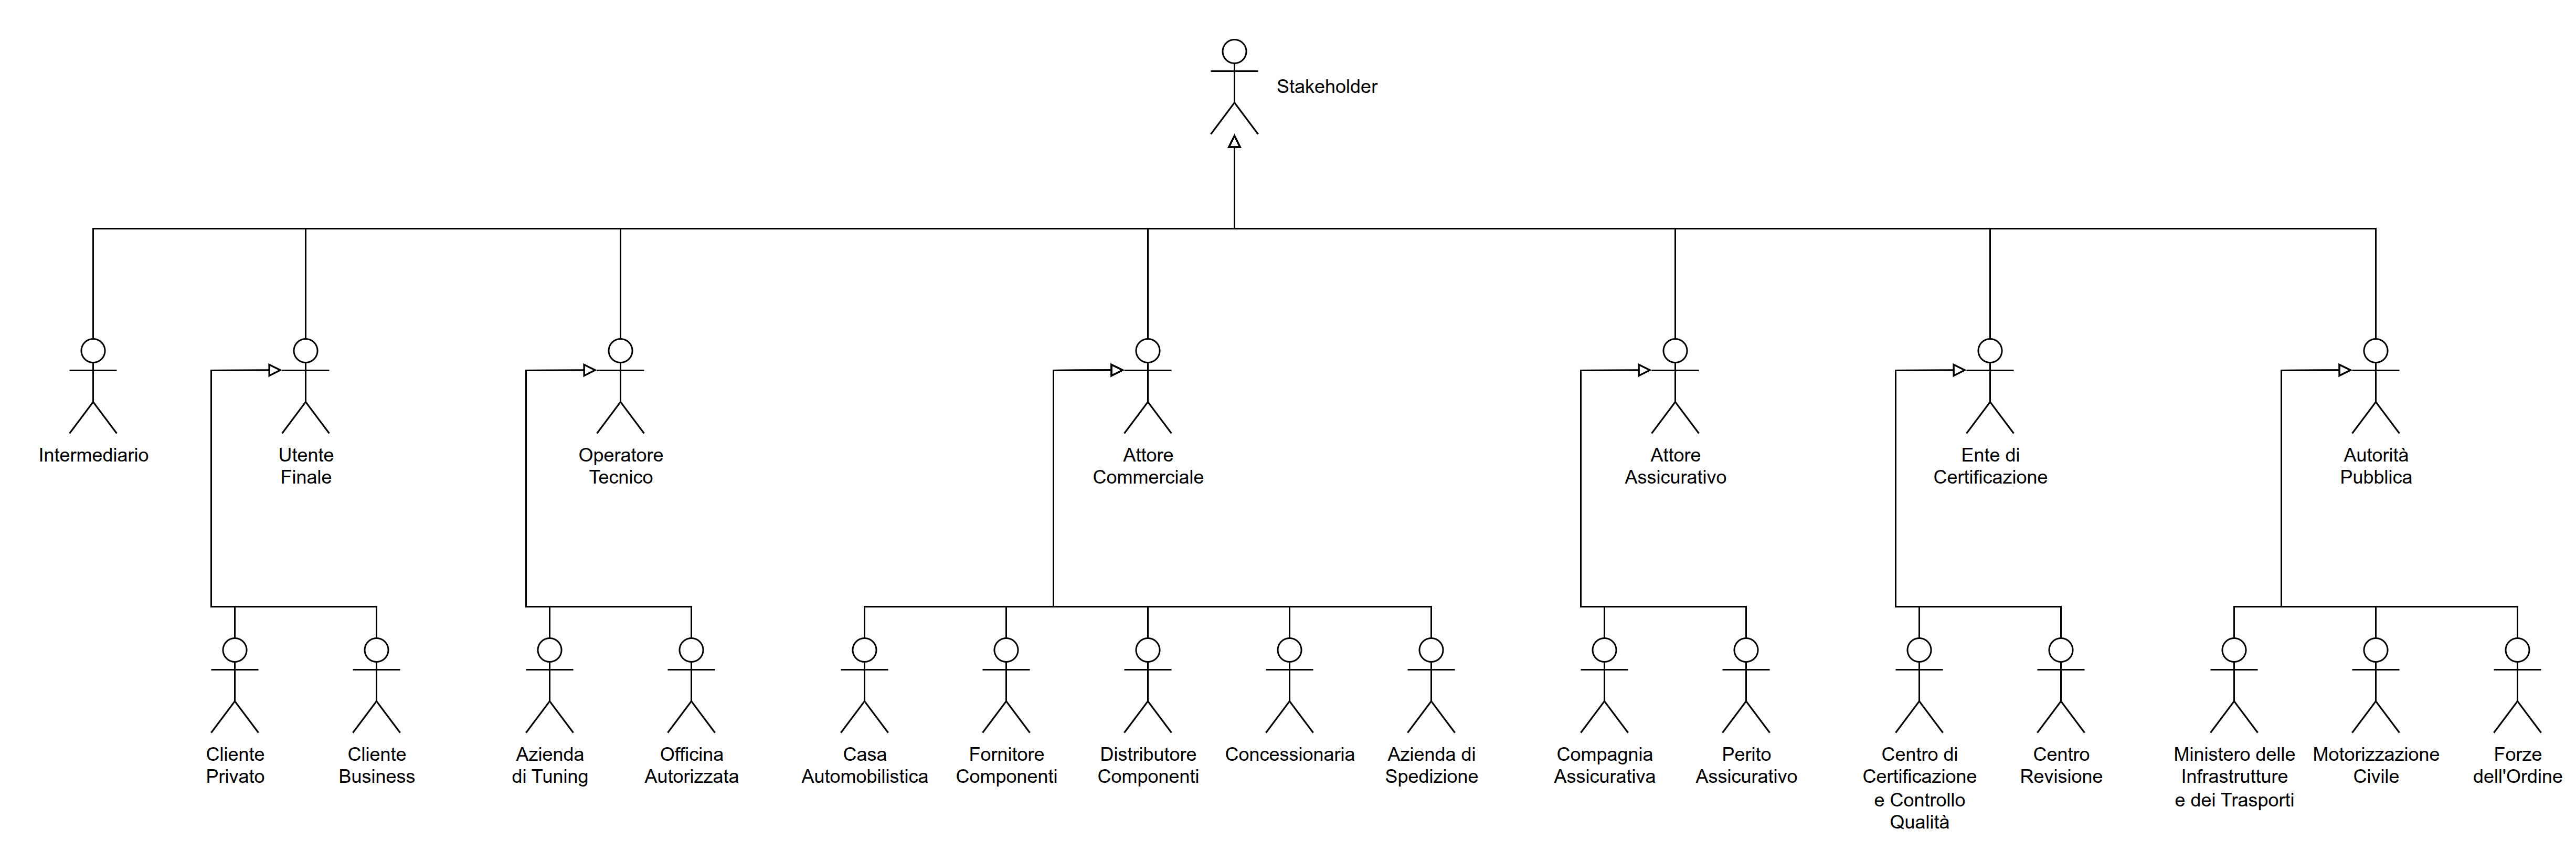
\includegraphics[width=1.3\textwidth]{imgs/context/stakeholders_diagram.png}}
    \caption{Stakeholder Diagram}
    \label{fig:stakeholder-diagram}
\end{figure}

Le categorie individuate, con i relativi attori specifici, sono le seguenti:

\begin{itemize}
    \item \textbf{Utente Finale}: raccoglie i soggetti che utilizzano il veicolo e ne subiscono direttamente le conseguenze in termini di sicurezza, valore e regolarit\`a amministrativa.
    \begin{itemize}
        \item \textit{Cliente Privato}: \`e l'utente finale che acquista il veicolo e commissiona le modifiche. Il suo interesse primario risiede nel disporre di un mezzo personalizzato, legalmente conforme e dotato di uno storico verificabile che ne tuteli il valore nel tempo.
        \item \textit{Cliente Business}: comprende le imprese e i gestori di flotte che impiegano veicoli commerciali allestiti o personalizzati. \`E interessato a dimostrare la conformit\`a dell'intero parco mezzi e a preservarne il valore residuo in sede di dismissione.
    \end{itemize}

    \item \textbf{Operatore Tecnico}: comprende i soggetti che intervengono materialmente sul veicolo.
    \begin{itemize}
        \item \textit{Azienda di Tuning}: esegue le modifiche funzionali ed estetiche commissionate. \`E interessata a valorizzare la qualit\`a del proprio operato e a tutelarsi da contestazioni infondate.
        \item \textit{Officina Autorizzata}: effettua interventi di manutenzione e installazione nel rispetto degli standard del costruttore. \`E interessata a dimostrare la conformit\`a delle lavorazioni eseguite.
    \end{itemize}

    \item \textbf{Attore Commerciale}: riunisce i soggetti che operano lungo la catena di fornitura e di distribuzione del veicolo e dei suoi componenti.
    \begin{itemize}
        \item \textit{Casa Automobilistica}: produce il veicolo base e ne detiene i dati ufficiali. \`E interessata alla tutela del marchio e al monitoraggio dell'impatto delle modifiche post-vendita sui propri mezzi.
        \item \textit{Fornitore Componenti}: produce la componentistica destinata alle modifiche ed \`e interessato ad attestare l'originalit\`a e le specifiche tecniche dei propri prodotti.
        \item \textit{Distributore Componenti}: cura la distribuzione dei ricambi verso officine e aziende di tuning, con interesse a dimostrare la tracciabilit\`a della merce trattata.
        \item \textit{Concessionaria}: rappresenta il punto di contatto commerciale con il cliente ed \`e interessata a offrire un servizio a valore aggiunto riducendo al contempo il rischio legale connesso alla vendita di veicoli modificati.
        \item \textit{Azienda di Spedizione}: cura la logistica di trasferimento del veicolo e della componentistica tra i diversi operatori della filiera, con interesse a documentare in modo incontestabile la presa in carico e la riconsegna del mezzo.
    \end{itemize}

    \item \textbf{Attore Assicurativo}: include i soggetti che assumono e valutano il rischio connesso alla circolazione del veicolo.
    \begin{itemize}
        \item \textit{Compagnia Assicurativa}: \`e interessata a disporre di informazioni attendibili sulle modifiche apportate, sia per una corretta valutazione del rischio in fase di sottoscrizione, sia per una gestione pi\`u rapida e oggettiva dei sinistri.
        \item \textit{Perito Assicurativo}: professionista incaricato di accertare lo stato del veicolo e l'entit\`a del danno in caso di sinistro. \`E interessato a ricostruire in modo rapido e attendibile la configurazione effettiva del mezzo al momento dell'evento.
    \end{itemize}

    \item \textbf{Ente di Certificazione}: raccoglie gli organismi terzi e accreditati che eseguono materialmente le verifiche tecniche sul veicolo e ne attestano la conformit\`a, rispondendo in proprio della correttezza del giudizio espresso. Il valore della loro attivit\`a dipende dal riconoscimento di cui gode il rispettivo accreditamento.
    \begin{itemize}
        \item \textit{Centro di Certificazione e Controllo Qualit\`a}: organismo terzo e imparziale che verifica la conformit\`a tecnica e normativa degli interventi, rilasciando la relativa certificazione. \`E l'unico soggetto della categoria che, nello scenario specifico definito nel Capitolo~3, opera direttamente sulla piattaforma.
        \item \textit{Centro Revisione}: esegue le verifiche periodiche obbligatorie ed \`e interessato a disporre di uno storico affidabile degli interventi subiti dal mezzo.
    \end{itemize}

    \item \textbf{Autorit\`a Pubblica}: comprende i soggetti titolari di potest\`a normativa e di vigilanza, cui competono la definizione delle regole tecniche, il riconoscimento formale delle modifiche e il controllo sulla sicurezza dei veicoli circolanti.
    \begin{itemize}
        \item \textit{Ministero delle Infrastrutture e dei Trasporti}: definisce il quadro normativo di riferimento in materia di omologazione e circolazione.
        \item \textit{Motorizzazione Civile}: \`e competente per l'aggiornamento della carta di circolazione e per il riconoscimento formale delle modifiche apportate.
        \item \textit{Forze dell'Ordine}: effettuano i controlli su strada ed \`e loro interesse poter verificare rapidamente la corrispondenza tra il veicolo e quanto risulta documentato.
    \end{itemize}
\end{itemize}

L'\textbf{Intermediario} \`e un soggetto specializzato nella gestione di piattaforme di tracciamento basate su DLT: fornisce l'infrastruttura tecnologica e funge da punto di contatto tecnico per tutti gli altri attori della filiera. Il suo interesse risiede nell'adozione della soluzione lungo l'intera catena del valore e nella sostenibilit\`a economica dell'esercizio, obiettivi che trovano espressione nei softgoal illustrati nel paragrafo seguente.

\subsection{Softgoal Diagram}

I \textbf{softgoal} rappresentano gli obiettivi non funzionali del sistema, ossia le qualit\`a che esso deve possedere per risultare accettabile e di successo agli occhi degli attori coinvolti. A differenza dei goal, essi non ammettono una verifica binaria di soddisfacimento, ma vengono perseguiti secondo un criterio di sufficienza.

Il diagramma riportato in Figura~\ref{fig:softgoal-diagram} \`e organizzato attorno a un softgoal radice, \textbf{Certificazione digitale affidabile delle modifiche ai veicoli}, che sintetizza la finalit\`a complessiva del sistema: garantire un ecosistema digitale sicuro e condiviso per la registrazione e la certificazione delle modifiche post-vendita dei veicoli attraverso l'utilizzo della tecnologia blockchain. A tale obiettivo generale concorrono trentacinque softgoal specifici, cinque per ciascuna delle sei categorie individuate e cinque propri dell'Intermediario; le linee continue collegano ogni softgoal allo stakeholder che ne \`e portatore.

\begin{figure}[H]
    \centering
    \makebox[\textwidth][c]{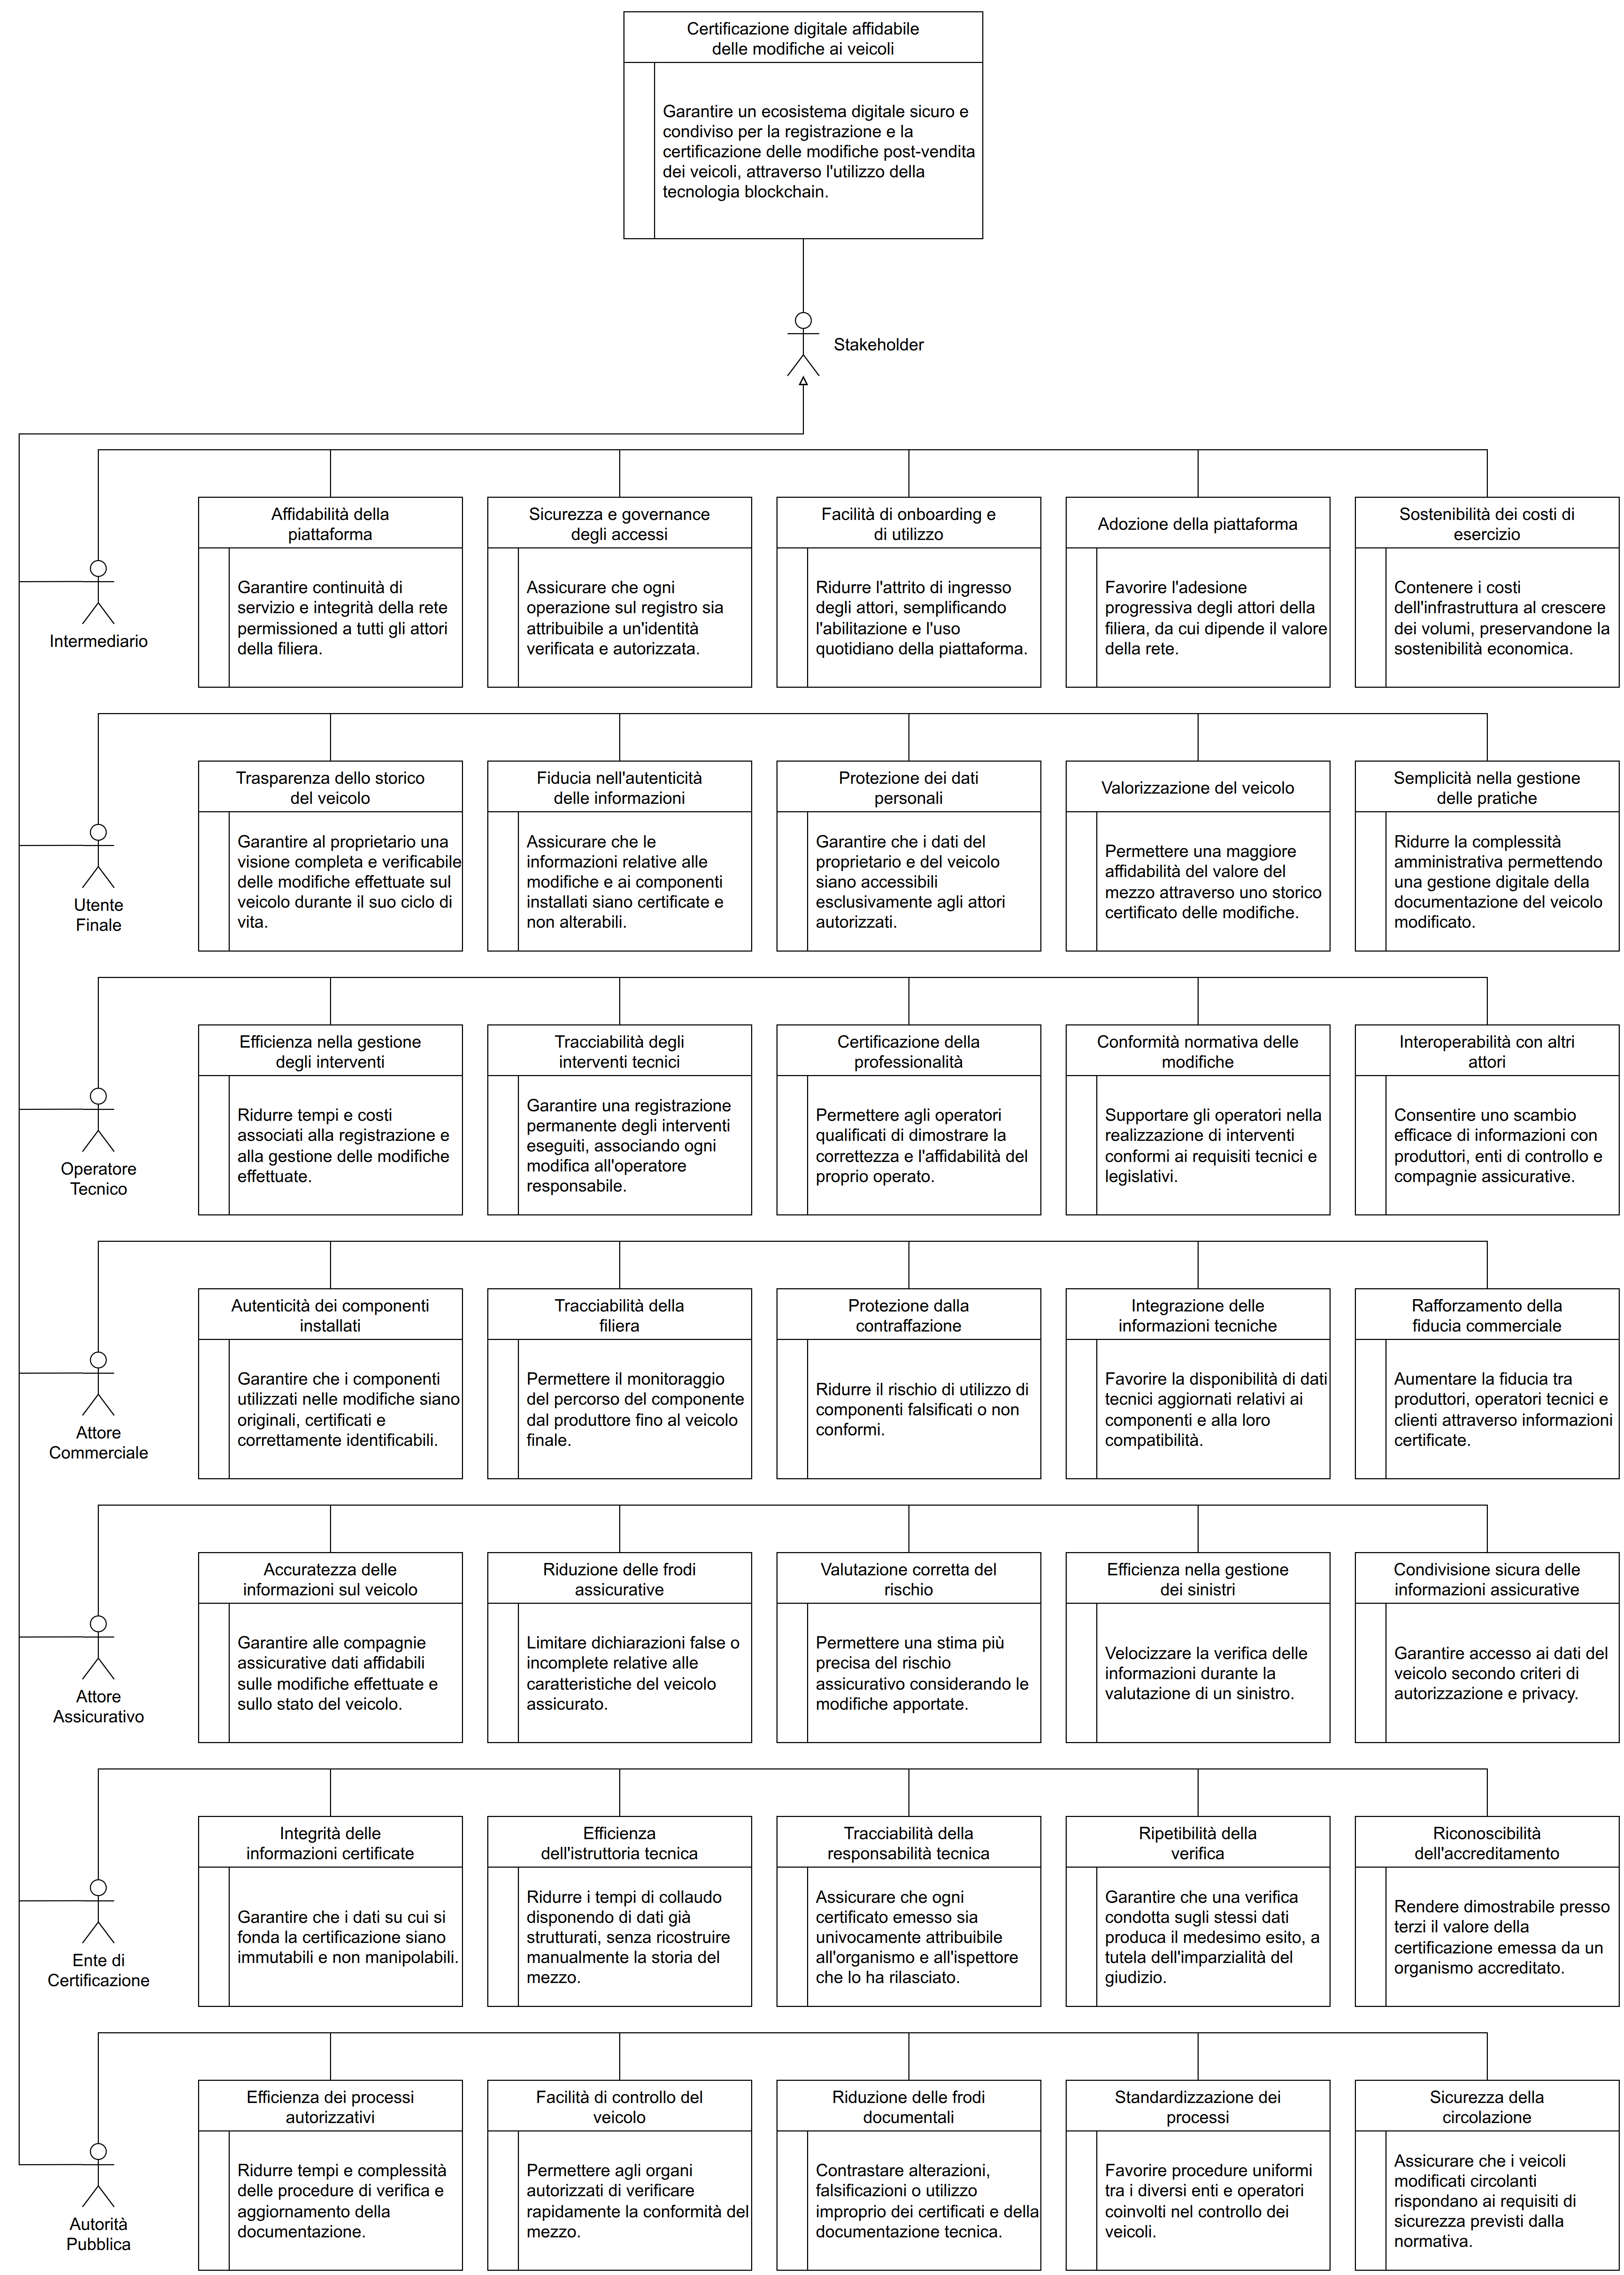
\includegraphics[height=0.85\textheight]{imgs/context/softgoal_diagram.png}}
    \caption{Softgoal Diagram}
    \label{fig:softgoal-diagram}
\end{figure}

\subsubsection*{Softgoal dell'Intermediario}

\begin{itemize}
    \item \textbf{Affidabilit\`a della piattaforma}: garantire continuit\`a di servizio e integrit\`a della rete permissioned a tutti gli attori della filiera.
    \item \textbf{Sicurezza e governance degli accessi}: assicurare che ogni operazione sul registro sia attribuibile a un'identit\`a verificata e autorizzata.
    \item \textbf{Facilit\`a di onboarding e di utilizzo}: ridurre l'attrito di ingresso degli attori, semplificando l'abilitazione e l'uso quotidiano della piattaforma.
    \item \textbf{Adozione della piattaforma}: favorire l'adesione progressiva degli attori della filiera, da cui dipende il valore della rete.
    \item \textbf{Sostenibilit\`a dei costi di esercizio}: contenere i costi dell'infrastruttura al crescere dei volumi, preservandone la sostenibilit\`a economica.
\end{itemize}

\subsubsection*{Softgoal dell'Utente Finale}

\begin{itemize}
    \item \textbf{Trasparenza dello storico del veicolo}: garantire al proprietario una visione completa e verificabile delle modifiche effettuate sul veicolo durante il suo ciclo di vita.
    \item \textbf{Fiducia nell'autenticit\`a delle informazioni}: assicurare che le informazioni relative alle modifiche e ai componenti installati siano certificate e non alterabili.
    \item \textbf{Protezione dei dati personali}: garantire che i dati del proprietario e del veicolo siano accessibili esclusivamente agli attori autorizzati.
    \item \textbf{Valorizzazione del veicolo}: permettere una maggiore affidabilit\`a del valore del mezzo attraverso uno storico certificato delle modifiche.
    \item \textbf{Semplicit\`a nella gestione delle pratiche}: ridurre la complessit\`a amministrativa permettendo una gestione digitale della documentazione del veicolo modificato.
\end{itemize}

\subsubsection*{Softgoal dell'Operatore Tecnico}

\begin{itemize}
    \item \textbf{Efficienza nella gestione degli interventi}: ridurre tempi e costi associati alla registrazione e alla gestione delle modifiche effettuate.
    \item \textbf{Tracciabilit\`a degli interventi tecnici}: garantire una registrazione permanente degli interventi eseguiti, associando ogni modifica all'operatore responsabile.
    \item \textbf{Certificazione della professionalit\`a}: permettere agli operatori qualificati di dimostrare la correttezza e l'affidabilit\`a del proprio operato.
    \item \textbf{Conformit\`a normativa delle modifiche}: supportare gli operatori nella realizzazione di interventi conformi ai requisiti tecnici e legislativi.
    \item \textbf{Interoperabilit\`a con altri attori}: consentire uno scambio efficace di informazioni con produttori, enti di controllo e compagnie assicurative.
\end{itemize}

\subsubsection*{Softgoal dell'Attore Commerciale}

\begin{itemize}
    \item \textbf{Autenticit\`a dei componenti installati}: garantire che i componenti utilizzati nelle modifiche siano originali, certificati e correttamente identificabili.
    \item \textbf{Tracciabilit\`a della filiera}: permettere il monitoraggio del percorso del componente dal produttore fino al veicolo finale.
    \item \textbf{Protezione dalla contraffazione}: ridurre il rischio di utilizzo di componenti falsificati o non conformi.
    \item \textbf{Integrazione delle informazioni tecniche}: favorire la disponibilit\`a di dati tecnici aggiornati relativi ai componenti e alla loro compatibilit\`a.
    \item \textbf{Rafforzamento della fiducia commerciale}: aumentare la fiducia tra produttori, operatori tecnici e clienti attraverso informazioni certificate.
\end{itemize}

\subsubsection*{Softgoal dell'Attore Assicurativo}

\begin{itemize}
    \item \textbf{Accuratezza delle informazioni sul veicolo}: garantire alle compagnie assicurative dati affidabili sulle modifiche effettuate e sullo stato del veicolo.
    \item \textbf{Riduzione delle frodi assicurative}: limitare dichiarazioni false o incomplete relative alle caratteristiche del veicolo assicurato.
    \item \textbf{Valutazione corretta del rischio}: permettere una stima pi\`u precisa del rischio assicurativo considerando le modifiche apportate.
    \item \textbf{Efficienza nella gestione dei sinistri}: velocizzare la verifica delle informazioni durante la valutazione di un sinistro.
    \item \textbf{Condivisione sicura delle informazioni assicurative}: garantire accesso ai dati del veicolo secondo criteri di autorizzazione e privacy.
\end{itemize}

\subsubsection*{Softgoal dell'Ente di Certificazione}

\begin{itemize}
    \item \textbf{Integrit\`a delle informazioni certificate}: garantire che i dati su cui si fonda la certificazione siano immutabili e non manipolabili.
    \item \textbf{Efficienza dell'istruttoria tecnica}: ridurre i tempi di collaudo disponendo di dati gi\`a strutturati, senza ricostruire manualmente la storia del mezzo.
    \item \textbf{Tracciabilit\`a della responsabilit\`a tecnica}: assicurare che ogni certificato emesso sia univocamente attribuibile all'organismo e all'ispettore che lo ha rilasciato.
    \item \textbf{Ripetibilit\`a della verifica}: garantire che una verifica condotta sugli stessi dati produca il medesimo esito, a tutela dell'imparzialit\`a del giudizio.
    \item \textbf{Riconoscibilit\`a dell'accreditamento}: rendere dimostrabile presso terzi il valore della certificazione emessa da un organismo accreditato.
\end{itemize}

\subsubsection*{Softgoal dell'Autorit\`a Pubblica}

\begin{itemize}
    \item \textbf{Efficienza dei processi autorizzativi}: ridurre tempi e complessit\`a delle procedure di verifica e aggiornamento della documentazione.
    \item \textbf{Facilit\`a di controllo del veicolo}: permettere agli organi autorizzati di verificare rapidamente la conformit\`a del mezzo.
    \item \textbf{Riduzione delle frodi documentali}: contrastare alterazioni, falsificazioni o utilizzo improprio dei certificati e della documentazione tecnica.
    \item \textbf{Standardizzazione dei processi}: favorire procedure uniformi tra i diversi enti e operatori coinvolti nel controllo dei veicoli.
    \item \textbf{Sicurezza della circolazione}: assicurare che i veicoli modificati circolanti rispondano ai requisiti di sicurezza previsti dalla normativa.
\end{itemize}

\subsection{Softgoal Dependency Diagram}

Il \textbf{Softgoal Dependency Diagram} riportato in Figura~\ref{fig:softgoal-dependency} sposta l'attenzione dalle singole qualit\`a alla rete di relazioni che intercorre tra di esse. Alle linee continue del diagramma precedente, che associano ciascun softgoal al proprio stakeholder, si affiancano qui frecce tratteggiate che rappresentano le dipendenze reciproche. Esse vanno interpretate come segue:

\begin{itemize}
    \item l'etichetta \textbf{``+'' (contributes)} indica una relazione di rinforzo: il softgoal da cui parte la coda della freccia favorisce la realizzazione del softgoal su cui ricade la testa;
    \item l'etichetta \textbf{``$-$'' (hinders)} indica una relazione di ostacolo: il perseguimento del primo softgoal rende pi\`u difficile il raggiungimento del secondo, evidenziando un \textit{trade-off} progettuale;
    \item le frecce con \textbf{doppia punta} rappresentano relazioni reciproche, nelle quali il rinforzo o l'ostacolo agisce in entrambe le direzioni.
\end{itemize}

\begin{figure}[H]
    \centering
    \makebox[\textwidth][c]{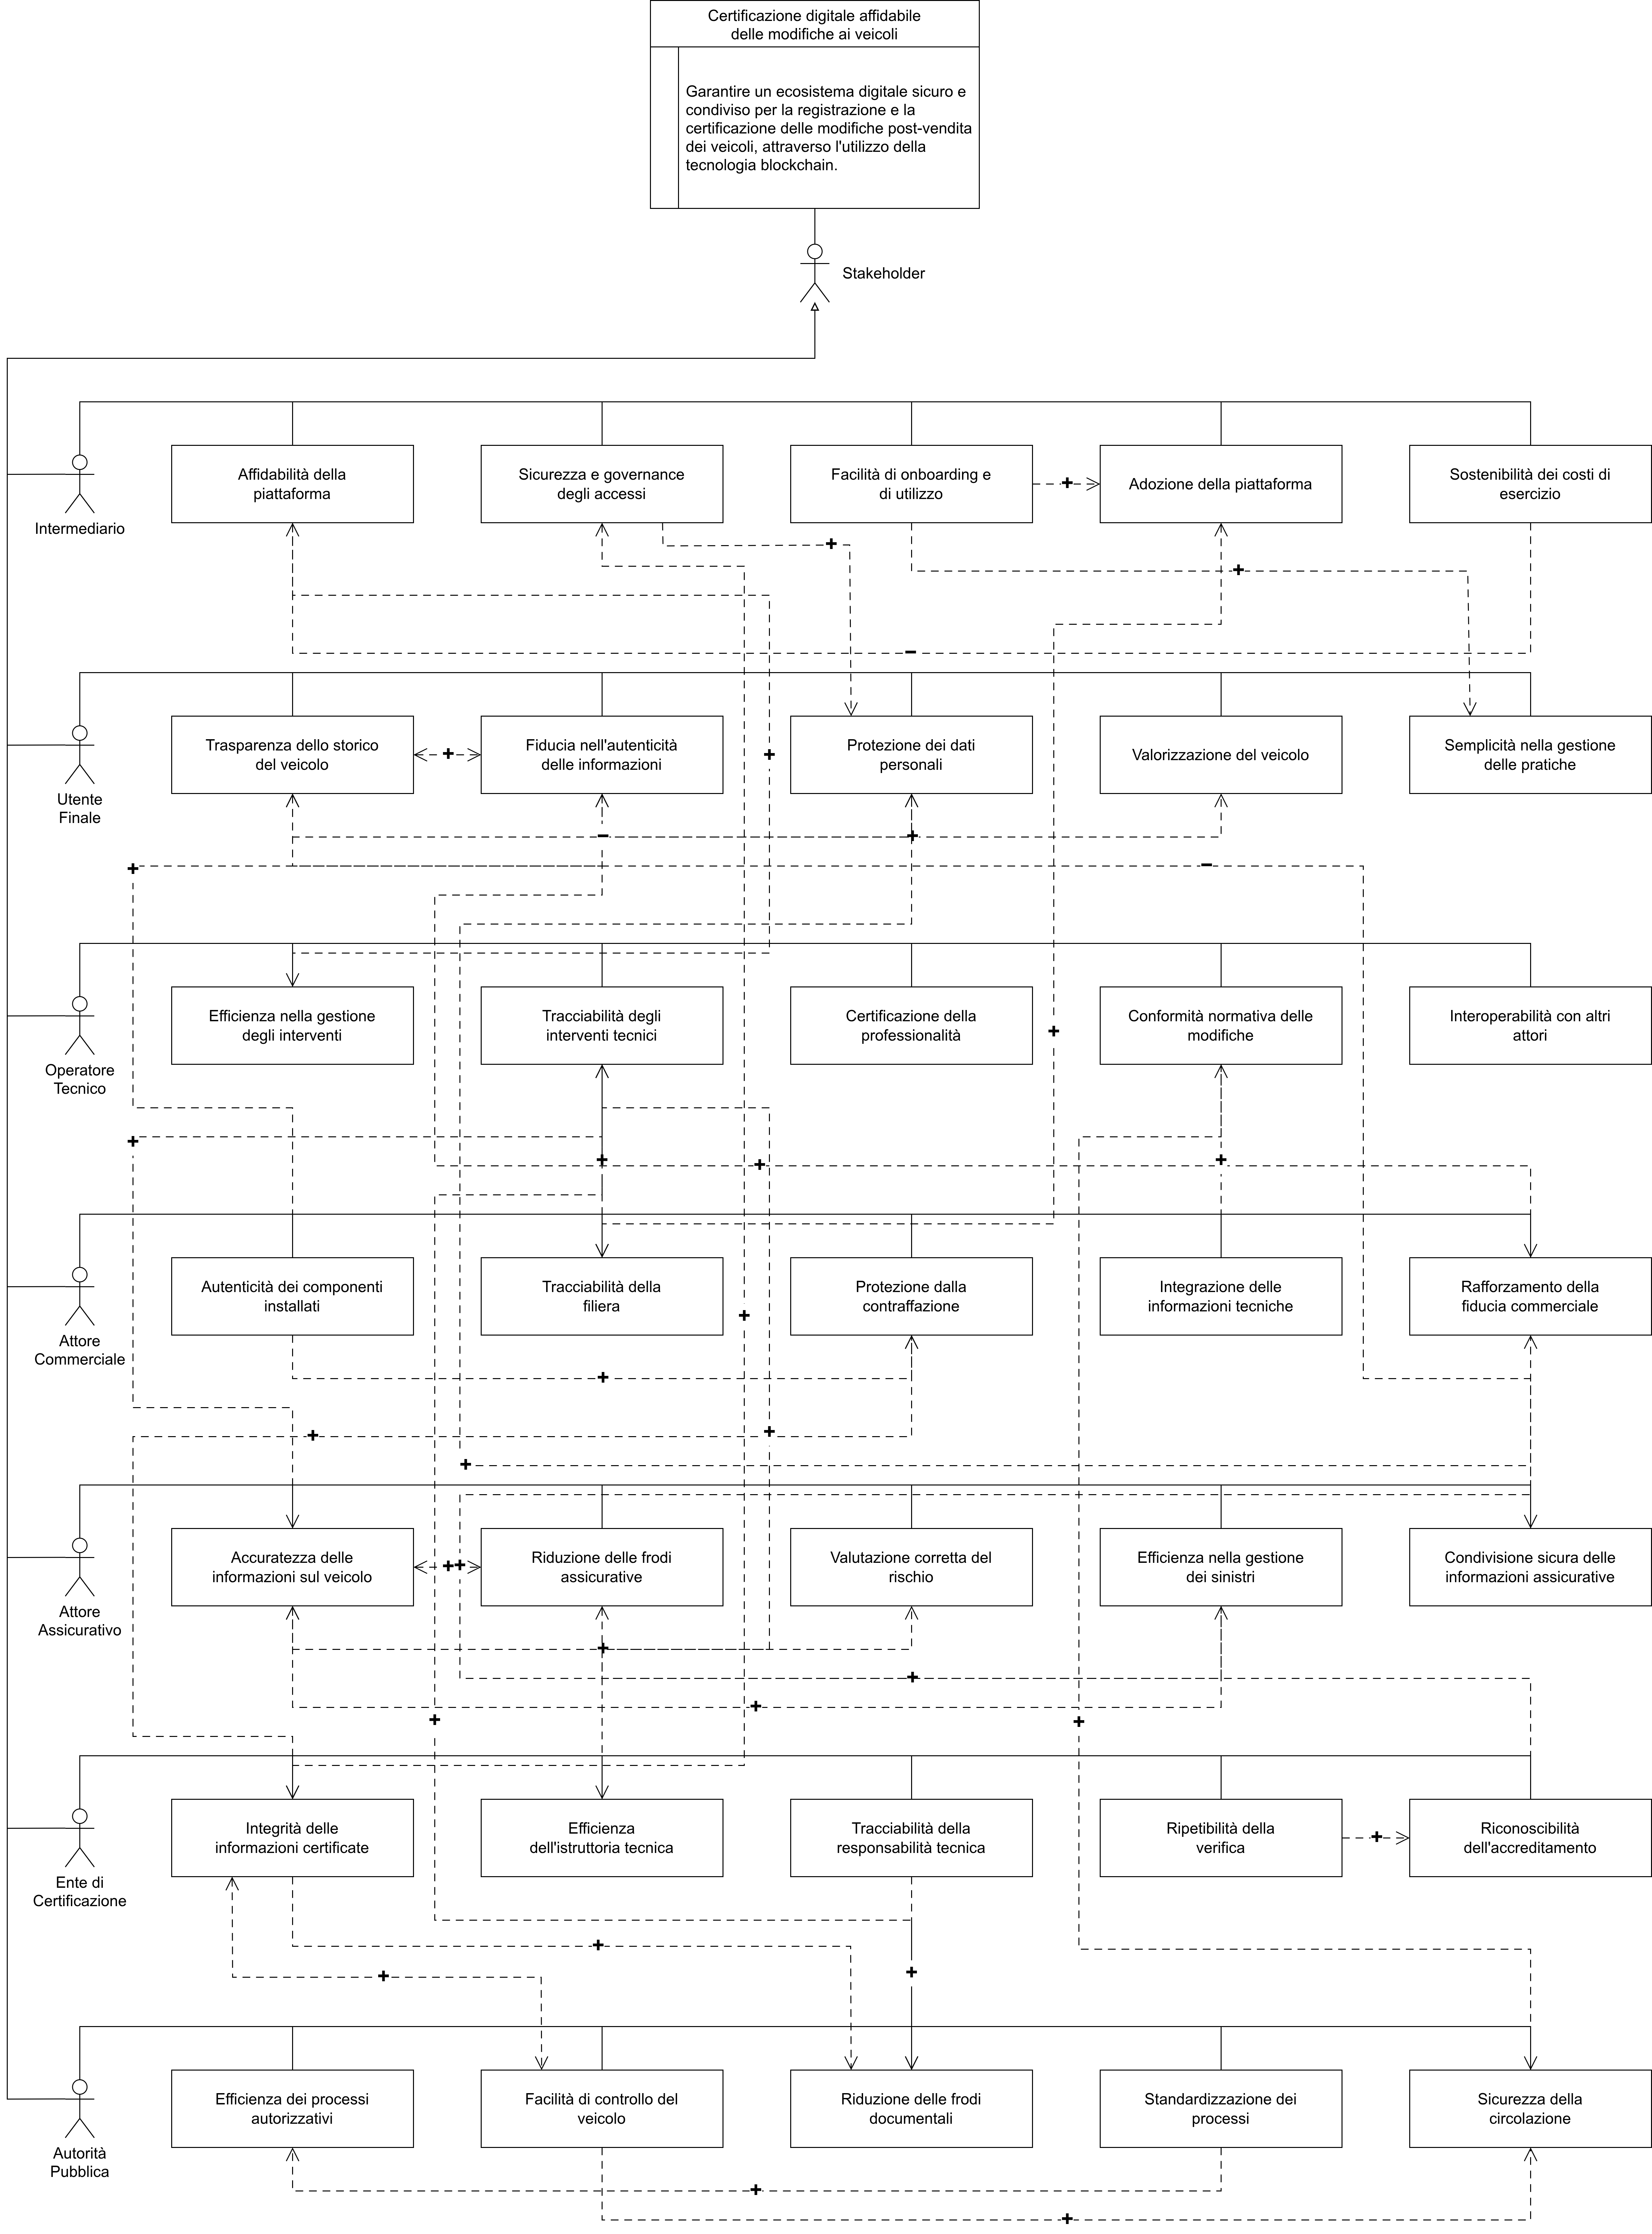
\includegraphics[height=0.85\textheight]{imgs/context/softgoal_dependency.png}}
    \caption{Softgoal Dependency Diagram}
    \label{fig:softgoal-dependency}
\end{figure}

Di seguito vengono analizzate nel dettaglio le singole dipendenze.

\subsubsection*{Contributes (+)}

\begin{itemize}
    \item \textbf{Trasparenza dello storico del veicolo \quad$+$\quad Fiducia nell'autenticit\`a delle informazioni} (reciproca)\\
    Una visione completa e consultabile della storia del mezzo alimenta la fiducia del proprietario nella veridicit\`a di quanto dichiarato; simmetricamente, la certezza che le informazioni non siano alterabili \`e ci\`o che rende la trasparenza effettivamente utile e non meramente formale.

    \item \textbf{Fiducia nell'autenticit\`a delle informazioni \quad$+$\quad Valorizzazione del veicolo} (reciproca)\\
    Il valore di mercato di un veicolo modificato dipende dalla possibilit\`a di dimostrare la regolarit\`a e la qualit\`a degli interventi subiti. Uno storico che gode di credibilit\`a presso gli acquirenti si traduce direttamente in una maggiore affidabilit\`a della stima del mezzo.

    \item \textbf{Autenticit\`a dei componenti installati \quad$+$\quad Fiducia nell'autenticit\`a delle informazioni}\\
    La certezza che i pezzi montati siano originali e correttamente identificati costituisce il presupposto sostanziale della fiducia: un registro accurato di lavorazioni eseguite con componenti non verificati resterebbe formalmente corretto ma privo di valore per il proprietario.

    \item \textbf{Autenticit\`a dei componenti installati \quad$+$\quad Protezione dalla contraffazione}\\
    L'identificazione univoca e certificata di ogni componente rende immediatamente riconoscibile la merce non conforme, riducendo lo spazio di mercato dei ricambi falsificati.

    \item \textbf{Tracciabilit\`a della filiera \quad$+$\quad Tracciabilit\`a degli interventi tecnici} (reciproca)\\
    Conoscere il percorso del componente dal produttore fino al veicolo completa l'informazione sull'intervento eseguito; a sua volta, la registrazione puntuale delle lavorazioni chiude l'ultimo anello della catena di tracciabilit\`a, collegando il pezzo al mezzo su cui \`e stato effettivamente installato.

    \item \textbf{Tracciabilit\`a degli interventi tecnici \quad$+$\quad Accuratezza delle informazioni sul veicolo}\\
    L'associazione permanente di ogni modifica all'operatore responsabile fornisce alle compagnie assicurative dati sullo stato del mezzo la cui provenienza \`e certa e verificabile.

    \item \textbf{Accuratezza delle informazioni sul veicolo \quad$+$\quad Valutazione corretta del rischio} (reciproca)\\
    La stima del rischio assicurativo non pu\`o essere pi\`u precisa dei dati su cui si fonda: disporre di informazioni affidabili sulle modifiche apportate \`e la condizione necessaria per una tariffazione aderente all'effettivo profilo del veicolo.

    \item \textbf{Accuratezza delle informazioni sul veicolo \quad$+$\quad Riduzione delle frodi assicurative} (reciproca)\\
    Quando lo stato del veicolo risulta da un registro non alterabile, lo spazio per dichiarazioni incomplete o mendaci in fase di sottoscrizione si riduce sensibilmente.

    \item \textbf{Riduzione delle frodi assicurative \quad$+$\quad Efficienza nella gestione dei sinistri} (reciproca)\\
    Il venir meno della necessit\`a di accertamenti approfonditi sulla veridicit\`a di quanto dichiarato accorcia i tempi di istruttoria; per converso, una verifica pi\`u rapida e sistematica in sede di sinistro scoraggia i comportamenti opportunistici.

    \item \textbf{Efficienza nella gestione dei sinistri \quad$+$\quad Accuratezza delle informazioni sul veicolo}\\
    La consultazione sistematica del registro in occasione di ogni sinistro alimenta e mantiene aggiornata la base informativa sullo stato effettivo dei veicoli assicurati.

    \item \textbf{Integrit\`a delle informazioni certificate \quad$+$\quad Facilit\`a di controllo del veicolo} (reciproca)\\
    Dati immutabili e non manipolabili consentono agli enti autorizzati di verificare la conformit\`a del mezzo senza dover ricostruire manualmente la documentazione, tanto durante i controlli su strada quanto in sede di revisione periodica.

    \item \textbf{Integrit\`a delle informazioni certificate \quad$+$\quad Riduzione delle frodi documentali}\\
    L'impossibilit\`a tecnica di alterare a posteriori una registrazione elimina alla radice le pratiche di falsificazione e di utilizzo improprio dei certificati di conformit\`a.

    \item \textbf{Integrit\`a delle informazioni certificate \quad$+$\quad Protezione dalla contraffazione} (reciproca)\\
    Il riscontro ufficiale dei dati di omologazione consente di individuare i componenti privi di certificazione valida, rafforzando l'azione di contrasto alla componentistica non conforme; a sua volta, una filiera dei ricambi non contraffatta garantisce che i dati sottoposti a omologazione corrispondano alla reale configurazione del mezzo.

    \item \textbf{Fiducia nell'autenticit\`a delle informazioni \quad$+$\quad Rafforzamento della fiducia commerciale}\\
    La credibilit\`a delle informazioni presso il cliente finale si riflette sull'intera filiera, migliorando il rapporto tra produttori, distributori, operatori tecnici e acquirenti.

    \item \textbf{Integrazione delle informazioni tecniche \quad$+$\quad Conformit\`a normativa delle modifiche}\\
    La disponibilit\`a di dati aggiornati sui componenti e sulla loro compatibilit\`a supporta l'operatore nella progettazione di interventi che rispettino fin dall'origine i requisiti tecnici e legislativi.


    \item \textbf{Protezione dei dati personali \quad$+$\quad Condivisione sicura delle informazioni assicurative} (reciproca)\\
    La definizione di criteri rigorosi di autorizzazione \`e ci\`o che rende praticabile la condivisione dei dati con le compagnie: senza un presidio credibile della riservatezza, l'accesso non sarebbe accettato dai proprietari. Simmetricamente, disciplinare l'accesso assicurativo secondo criteri espliciti rafforza la protezione complessiva dei dati del proprietario.

    \item \textbf{Riduzione delle frodi documentali \quad$+$\quad Tracciabilit\`a degli interventi tecnici} (reciproca)\\
    Il contrasto alla falsificazione documentale valorizza la registrazione puntuale delle lavorazioni, che a sua volta costituisce lo strumento operativo attraverso cui le alterazioni vengono rese rilevabili.

    \item \textbf{Sicurezza e governance degli accessi \quad$+$\quad Protezione dei dati personali}\\
    La verifica delle identit\`a e le politiche di autorizzazione definite dall'Intermediario costituiscono il presidio tecnico su cui si regge la riservatezza dei dati del proprietario: senza un controllo puntuale di chi accede a che cosa, ogni garanzia di privacy resterebbe una dichiarazione di intenti.

    \item \textbf{Sicurezza e governance degli accessi \quad$+$\quad Integrit\`a delle informazioni certificate} (reciproca)\\
    Solo operazioni attribuibili a soggetti verificati producono registrazioni su cui un organismo possa fondare una certificazione; simmetricamente, l'immutabilit\`a del dato certificato \`e ci\`o che rende sensato il presidio sugli accessi.

    \item \textbf{Affidabilit\`a della piattaforma \quad$+$\quad Efficienza nella gestione degli interventi}\\
    Continuit\`a di servizio e prestazioni stabili sono la precondizione perch\'e l'operatore registri le lavorazioni contestualmente all'esecuzione, senza che l'adempimento digitale rallenti il ciclo di lavoro in officina.

    \item \textbf{Facilit\`a di onboarding e di utilizzo \quad$+$\quad Adozione della piattaforma}\\
    Un processo di abilitazione semplice abbassa la soglia di ingresso e accelera l'adesione degli attori alla rete, in particolare delle realt\`a di piccole dimensioni prive di strutture informatiche interne.

    \item \textbf{Facilit\`a di onboarding e di utilizzo \quad$+$\quad Semplicit\`a nella gestione delle pratiche}\\
    Un'interfaccia immediata riduce l'onere amministrativo percepito dal proprietario nella gestione della documentazione del mezzo.

    \item \textbf{Adozione della piattaforma \quad$+$\quad Tracciabilit\`a della filiera} (reciproca)\\
    Il valore di un registro condiviso cresce con il numero di attori che vi partecipano: la tracciabilit\`a dal produttore al veicolo \`e conseguibile solo se tutti gli anelli della catena vi aderiscono e, a sua volta, una filiera effettivamente tracciata rende conveniente l'adesione di chi ancora ne \`e fuori.

    \item \textbf{Tracciabilit\`a degli interventi tecnici \quad$+$\quad Efficienza dell'istruttoria tecnica}\\
    Disporre di lavorazioni gi\`a registrate e attribuite al rispettivo operatore evita all'organismo di certificazione di ricostruire manualmente la storia del mezzo, abbreviando sensibilmente l'istruttoria che precede il collaudo.

    \item \textbf{Ripetibilit\`a della verifica \quad$+$\quad Riconoscibilit\`a dell'accreditamento}\\
    Un giudizio tecnico riproducibile a parit\`a di dati \`e ci\`o che rende credibile, e quindi spendibile presso terzi, l'accreditamento dell'organismo che lo emette.

    \item \textbf{Riconoscibilit\`a dell'accreditamento \quad$+$\quad Rafforzamento della fiducia commerciale}\\
    Il riconoscimento di cui gode l'organismo che certifica si trasferisce sulla reputazione dell'intera filiera che ne utilizza i certificati.

    \item \textbf{Tracciabilit\`a della responsabilit\`a tecnica \quad$+$\quad Riduzione delle frodi documentali}\\
    L'attribuzione univoca di ogni certificato all'organismo e all'ispettore che lo ha emesso rende immediatamente individuabile ogni documento apocrifo o rilasciato da soggetti non abilitati.

    \item \textbf{Standardizzazione dei processi \quad$+$\quad Efficienza dei processi autorizzativi}\\
    Procedure uniformi tra enti diversi eliminano le duplicazioni istruttorie e accorciano i tempi delle autorizzazioni.

    \item \textbf{Facilit\`a di controllo del veicolo \quad$+$\quad Sicurezza della circolazione}\\
    Controlli su strada rapidi e non ambigui aumentano la probabilit\`a di intercettare i veicoli non conformi prima che si traducano in un pericolo per la circolazione.

    \item \textbf{Conformit\`a normativa delle modifiche \quad$+$\quad Sicurezza della circolazione}\\
    Interventi progettati fin dall'origine nel rispetto dei requisiti tecnici e legislativi riducono alla fonte il numero di mezzi irregolari immessi in circolazione.
\end{itemize}

\subsubsection*{Hinders ($-$)}

\begin{itemize}
    \item \textbf{Trasparenza dello storico del veicolo \quad$-$\quad Protezione dei dati personali} (reciproca)\\
    Si tratta del principale \textit{trade-off} del sistema. Ogni ampliamento della visibilit\`a sullo storico del mezzo comporta l'esposizione di informazioni riconducibili al proprietario e alle sue abitudini; per converso, ogni restrizione posta a tutela della riservatezza riduce la completezza dell'informazione effettivamente consultabile. Il conflitto non pu\`o essere risolto a favore di uno dei due obiettivi, ma va governato attraverso politiche di accesso selettivo che differenzino i dati visibili in funzione del ruolo del richiedente.

    \item \textbf{Condivisione sicura delle informazioni assicurative \quad$-$\quad Trasparenza dello storico del veicolo}\\
    I vincoli di autorizzazione e di \textit{privacy} che regolano l'accesso delle compagnie ai dati del veicolo, pur necessari, introducono filtri che limitano la visione complessiva dello storico disponibile agli altri attori, riducendo il grado di trasparenza effettivamente conseguibile.

    \item \textbf{Sostenibilit\`a dei costi di esercizio \quad$-$\quad Affidabilit\`a della piattaforma}\\
    Il contenimento dei costi dell'infrastruttura comprime i margini di ridondanza e di capacit\`a con cui si garantisce la continuit\`a del servizio. \`E il \textit{trade-off} tipico di un'infrastruttura distribuita e ricade interamente sull'Intermediario, che deve individuare il punto di equilibrio tra livello di servizio offerto e costo per transazione registrata.
\end{itemize}

Nel complesso, la rete di dipendenze evidenzia come le qualit\`a attese dai diversi stakeholder siano largamente convergenti: la quasi totalit\`a delle relazioni \`e di tipo \textit{contributes}, a conferma del fatto che un registro condiviso e non alterabile produce benefici simultanei lungo tutta la filiera. Le tre relazioni di ostacolo individuate segnalano altrettanti vincoli progettuali. Le prime due ruotano attorno alla tensione tra apertura informativa e riservatezza, che si conferma il \textit{trade-off} pi\`u delicato da governare nelle fasi successive di definizione dell'architettura e delle politiche di accesso; la terza riguarda l'Intermediario e contrappone il livello di servizio garantito al costo dell'infrastruttura che lo sostiene, questione che sar\`a ripresa nel Capitolo~7 in sede di valutazione economica.

\chapter{Descrizione dello Scenario Specifico dell'Idea Progettuale}

\section{Lo scenario specifico}

L'analisi del contesto svolta nel capitolo precedente ha delineato un quadro ampio, comprensivo di tutti i soggetti che, a vario titolo, gravitano attorno al mondo dell'automotive tuning. Al fine di definire un'idea progettuale concreta e realizzabile, è necessario restringere tale quadro a uno \textbf{scenario specifico}, individuando gli attori che interagiscono direttamente con la piattaforma e i ruoli da essi assunti all'interno del sistema.

Il settore della personalizzazione dei veicoli ha assunto negli ultimi anni una rilevanza economica crescente, accompagnata però da una persistente opacità informativa. Le modifiche apportate a un veicolo --- interventi sulla meccanica, sull'assetto, sull'impianto frenante o sull'estetica --- vengono documentate attraverso fatture, dichiarazioni di conformità e annotazioni sul libretto di circolazione, ossia strumenti eterogenei, facilmente smarribili e non verificabili in modo indipendente. Al momento della rivendita, l'acquirente non dispone di alcuno strumento affidabile per accertare quali lavorazioni siano state realmente eseguite, da chi, con quali componenti e nel rispetto di quali requisiti di omologazione.

Questa asimmetria informativa produce conseguenze concrete su tutta la filiera: l'Azienda di Tuning non riesce a valorizzare la qualità del proprio operato né a tutelarsi da contestazioni infondate; la Concessionaria assume un rischio legale nel commercializzare un veicolo modificato di cui non può dimostrare la piena conformità; il Centro di Certificazione deve ricostruire manualmente la storia degli interventi prima di poter procedere al collaudo; il Cliente Privato, infine, subisce una perdita di valore del proprio veicolo al momento della rivendita, non potendo dimostrare la regolarità e la qualità delle personalizzazioni.

L'idea progettuale, denominata \textit{Tuning Ledger}, risponde a queste criticità attraverso il \textbf{Digital Modified Vehicle Passport} (DMVP): un passaporto digitale immutabile, associato univocamente al numero di telaio del veicolo, che accompagna il mezzo lungo l'intero ciclo di vita registrando in modo verificabile ogni modifica e ogni certificazione. La piattaforma adotta un'architettura ibrida, nella quale i dati descrittivi e la documentazione voluminosa risiedono in un database \textit{off-chain}, mentre sulla blockchain viene ancorata la sola impronta crittografica (\textit{hash}) che ne garantisce l'integrità.

La piattaforma è concepita per offrire servizi personalizzati ai seguenti stakeholder:

\begin{enumerate}
    \item \textbf{Intermediario}, in quanto soggetto che sviluppa e gestisce la piattaforma, interessato a fornire un'infrastruttura di tracciabilità affidabile agli attori della filiera e a verticalizzare la soluzione sulle loro specifiche esigenze.
    \item \textbf{Concessionaria}, in quanto interessata a differenziare la propria offerta commerciale con un servizio premium e a ridurre il rischio legale connesso alla vendita di veicoli modificati, potendo dimostrare la conformità di ogni intervento.
    \item \textbf{Azienda di Tuning}, in quanto interessata ad attestare digitalmente la qualità del proprio lavoro, tutelandosi da contestazioni infondate attraverso la registrazione immutabile delle lavorazioni eseguite e dei componenti installati.
    \item \textbf{Centro di Certificazione}, in quanto interessato a disporre di dati verificabili e già strutturati per l'esecuzione del collaudo, riducendo i tempi di verifica, e a registrare i certificati emessi in modo che siano controllabili da terzi.
    \item \textbf{Cliente Privato}, in quanto interessato a verificare l'autenticità delle modifiche apportate al proprio veicolo e a disporre di uno storico certificato e trasferibile, che ne accresce il valore al momento della rivendita.
\end{enumerate}

Restano invece esclusi dallo scenario specifico, pur essendo stati individuati nell'analisi del contesto, i soggetti che non interagiscono direttamente con la piattaforma ma con i quali essa si interfaccia in qualità di \textbf{partner}: la Motorizzazione Civile, competente per l'omologazione delle modifiche; la Casa Automobilistica, che fornisce i dati ufficiali del veicolo base; i Fornitori di componenti, che ne attestano la provenienza; e le Aziende di spedizione, coinvolte nella logistica di consegna.

\section{Contesto tecnologico: tecnologie e soluzioni già disponibili}

\subsection{Tecnologie rilevanti}

Il contesto tecnologico dell'idea progettuale è caratterizzato dalla necessità di gestire informazioni critiche relative al ciclo di vita dei veicoli, in particolare per quanto riguarda modifiche, manutenzioni e interventi certificati. In tale scenario risulta fondamentale adottare soluzioni in grado di garantire \textbf{integrità, tracciabilità e verificabilità} dei dati, riducendo le asimmetrie informative tra i diversi attori coinvolti.

In questo ambito la \textbf{blockchain} si configura come una tecnologia rilevante per lo sviluppo di sistemi informativi distribuiti orientati alla collaborazione tra organizzazioni. Essa può essere definita come un \textbf{registro distribuito} (\textit{Distributed Ledger Technology}, DLT) in cui le informazioni vengono registrate in modo immutabile e condiviso tra più nodi della rete, senza la necessità di un'autorità centrale di controllo. Le principali caratteristiche di interesse per il progetto sono:

\begin{itemize}
    \item \textbf{immutabilità dei dati}, che garantisce la non alterabilità delle informazioni storiche;
    \item \textbf{tracciabilità}, che consente di ricostruire in modo affidabile l'evoluzione delle modifiche apportate a un veicolo;
    \item \textbf{sicurezza}, ottenuta tramite meccanismi crittografici;
    \item \textbf{condivisione controllata}, che permette a più attori di accedere a un'unica fonte informativa affidabile.
\end{itemize}

Un elemento centrale della blockchain è il \textbf{meccanismo di consenso}, attraverso il quale i partecipanti alla rete concordano sulla validità delle informazioni da registrare. Tale meccanismo consente di garantire l'affidabilità del sistema anche in contesti caratterizzati da interessi differenti tra gli stakeholder, come è appunto il caso della filiera del tuning.

Dal punto di vista architetturale è possibile distinguere blockchain \textbf{pubbliche}, aperte e completamente decentralizzate; blockchain \textbf{private}, controllate da un singolo soggetto; e blockchain \textbf{permissioned}, in cui l'accesso è riservato a partecipanti autorizzati. Nel contesto automotive queste ultime risultano particolarmente rilevanti, poiché permettono di bilanciare decentralizzazione e controllo, consentendo la definizione di ruoli e responsabilità per soggetti quali officine, concessionarie ed enti certificatori.

Un ulteriore aspetto tecnologico di rilievo è rappresentato dagli \textbf{smart contract}, programmi eseguiti automaticamente sulla blockchain al verificarsi di determinate condizioni. Essi consentono di automatizzare i processi di validazione e certificazione, riducendo l'intervento manuale e aumentando l'affidabilità delle operazioni. L'integrazione con \textbf{oracoli} permette inoltre di collegare la blockchain a fonti informative esterne, quali gli enti di omologazione.

Nonostante i vantaggi, l'adozione della blockchain introduce alcune criticità, tra cui una maggiore \textbf{complessità architetturale}, la necessità di \textbf{competenze specialistiche} e potenziali \textbf{limiti di scalabilità} in scenari ad alto volume di transazioni. Alla luce di tali considerazioni, la blockchain emerge come tecnologia adeguata all'idea progettuale a condizione che venga adottata in modo mirato e integrata all'interno di un'architettura più ampia, coerente con i requisiti funzionali e organizzativi del sistema informativo.

\subsection{Soluzioni tecnologiche specifiche esistenti}

L'analisi delle soluzioni tecnologiche specifiche si basa sulla valutazione di piattaforme blockchain già adottate in contesti reali affini all'idea progettuale. L'obiettivo è verificare l'esistenza di tecnologie consolidate in grado di soddisfare i casi d'uso individuati, riducendo i rischi di sviluppo e aumentando l'affidabilità complessiva del sistema. I principali requisiti tecnologici del progetto possono essere sintetizzati nell'immutabilità e tracciabilità delle modifiche, nel coinvolgimento di più attori con ruoli distinti, nella verificabilità delle informazioni da parte di terzi, nell'integrazione con sistemi esterni e nella scalabilità con contenimento dei costi operativi.

Nel panorama delle soluzioni esistenti, piattaforme blockchain \textbf{permissioned} come \textbf{Hyperledger Fabric}~\cite{hyperledger} risultano già adottate in ambito automotive per la gestione di registri distribuiti relativi alla storia dei veicoli. Tali soluzioni consentono di registrare in modo sicuro eventi quali manutenzioni, restauri e trasferimenti di proprietà, garantendo trasparenza e immutabilità delle informazioni tra produttori, officine e assicurazioni. L'impiego di Hyperledger Fabric si è dimostrato efficace anche nella documentazione certificata dei processi di restauro delle auto classiche, promuovendo collaborazione, fiducia e aumento del valore di mercato dei veicoli~\cite{murta2024}.

Accanto alle soluzioni permissioned sono stati proposti anche approcci basati su blockchain pubbliche. Un esempio rilevante è rappresentato da architetture che prevedono la \textbf{tokenizzazione del veicolo} tramite l'emissione di un \textbf{NFT} associato al bene fisico~\cite{nftvehicle}: in tali modelli l'intero ciclo di vita del veicolo viene rappresentato attraverso smart contract gerarchici, che registrano transazioni e modifiche in modo strutturato, riducendo il rischio di frodi e asimmetrie informative. Queste soluzioni, spesso implementate su piattaforme come Ethereum, dimostrano la fattibilità tecnica del modello, pur presentando limiti in termini di costi e scalabilità.

Nel contesto dell'automotive tuning l'adozione di una piattaforma blockchain permissioned risulta particolarmente vantaggiosa. Un sistema come il DMVP consente di registrare modifiche estetiche e funzionali corredate dalle relative certificazioni normative, rendendo tali informazioni accessibili tramite applicazioni dedicate o QR code applicato al veicolo. L'utilizzo di smart contract permette inoltre di validare automaticamente la conformità delle modifiche, riducendo il rischio di irregolarità.

Alla luce di queste considerazioni, la soluzione tecnologica più adeguata consiste nell'adozione di una \textbf{blockchain permissioned} integrata all'interno di una piattaforma proprietaria, secondo un'\textbf{architettura ibrida} in cui la blockchain è utilizzata per la registrazione certificata e verificabile delle informazioni critiche, mentre la piattaforma applicativa gestisce la logica di business, l'interazione con gli utenti e l'integrazione con i sistemi esterni. Tale approccio consente di sfruttare tecnologie già validate in ambito automotive, garantendo al contempo flessibilità, controllo dei costi e copertura completa dei requisiti funzionali del progetto.

\section{Modellazione dello Scenario Specifico in GOREM}

Dall'analisi del contesto è stato definito uno scenario specifico che permette di identificare con precisione gli stakeholder direttamente coinvolti nello sviluppo e nell'uso della piattaforma e i diversi ruoli da essi assunti all'interno del sistema. In particolare:

\begin{enumerate}
    \item \textbf{Intermediario}
    \begin{itemize}
        \item \textit{Amministratore della piattaforma}: garantisce il funzionamento, la configurazione e la sicurezza della rete blockchain permissioned, definendo i canali e le politiche di validazione delle transazioni.
        \item \textit{Gestore delle identità e onboarding}: registra e verifica le identità degli attori business, abilitandoli all'uso della piattaforma ed emettendo le credenziali necessarie a operare sulla rete.
        \item \textit{Assistente all'uso}: fornisce assistenza tecnica e operativa agli utenti della piattaforma, accompagnandoli nella configurazione iniziale e nella risoluzione delle anomalie.
    \end{itemize}
    \item \textbf{Concessionaria}
    \begin{itemize}
        \item \textit{Registrante del veicolo base}: registra i dati identificativi del veicolo originale e la richiesta di tuning, creando il passaporto digitale associato al numero di telaio.
        \item \textit{Responsabile della consegna}: consegna il veicolo omologato al Cliente Privato e registra la consegna sul DMVP.
    \end{itemize}
    \item \textbf{Azienda di Tuning}
    \begin{itemize}
        \item \textit{Esecutore della modifica}: esegue le lavorazioni sul veicolo e ne carica in modo permanente la documentazione tecnica, comprensiva dei seriali dei componenti installati.
    \end{itemize}
    \item \textbf{Centro di Certificazione}
    \begin{itemize}
        \item \textit{Ispettore/Collaudatore}: verifica la conformità tecnica e normativa degli interventi eseguiti sul veicolo.
        \item \textit{Emittente della certificazione}: rilascia il certificato di conformità e lo registra in modo immutabile sulla piattaforma.
    \end{itemize}
    \item \textbf{Cliente Privato}
    \begin{itemize}
        \item \textit{Consultatore dello storico}: consulta in qualsiasi momento lo storico immutabile e completo delle modifiche del veicolo.
        \item \textit{Acquirente/Nuovo proprietario}: accetta il veicolo al termine della consegna e ne riceve la proprietà del passaporto digitale.
    \end{itemize}
\end{enumerate}

Quanto descritto è illustrato nella Figura~\ref{fig:role-diagram}.

\begin{figure}[H]
    \centering
    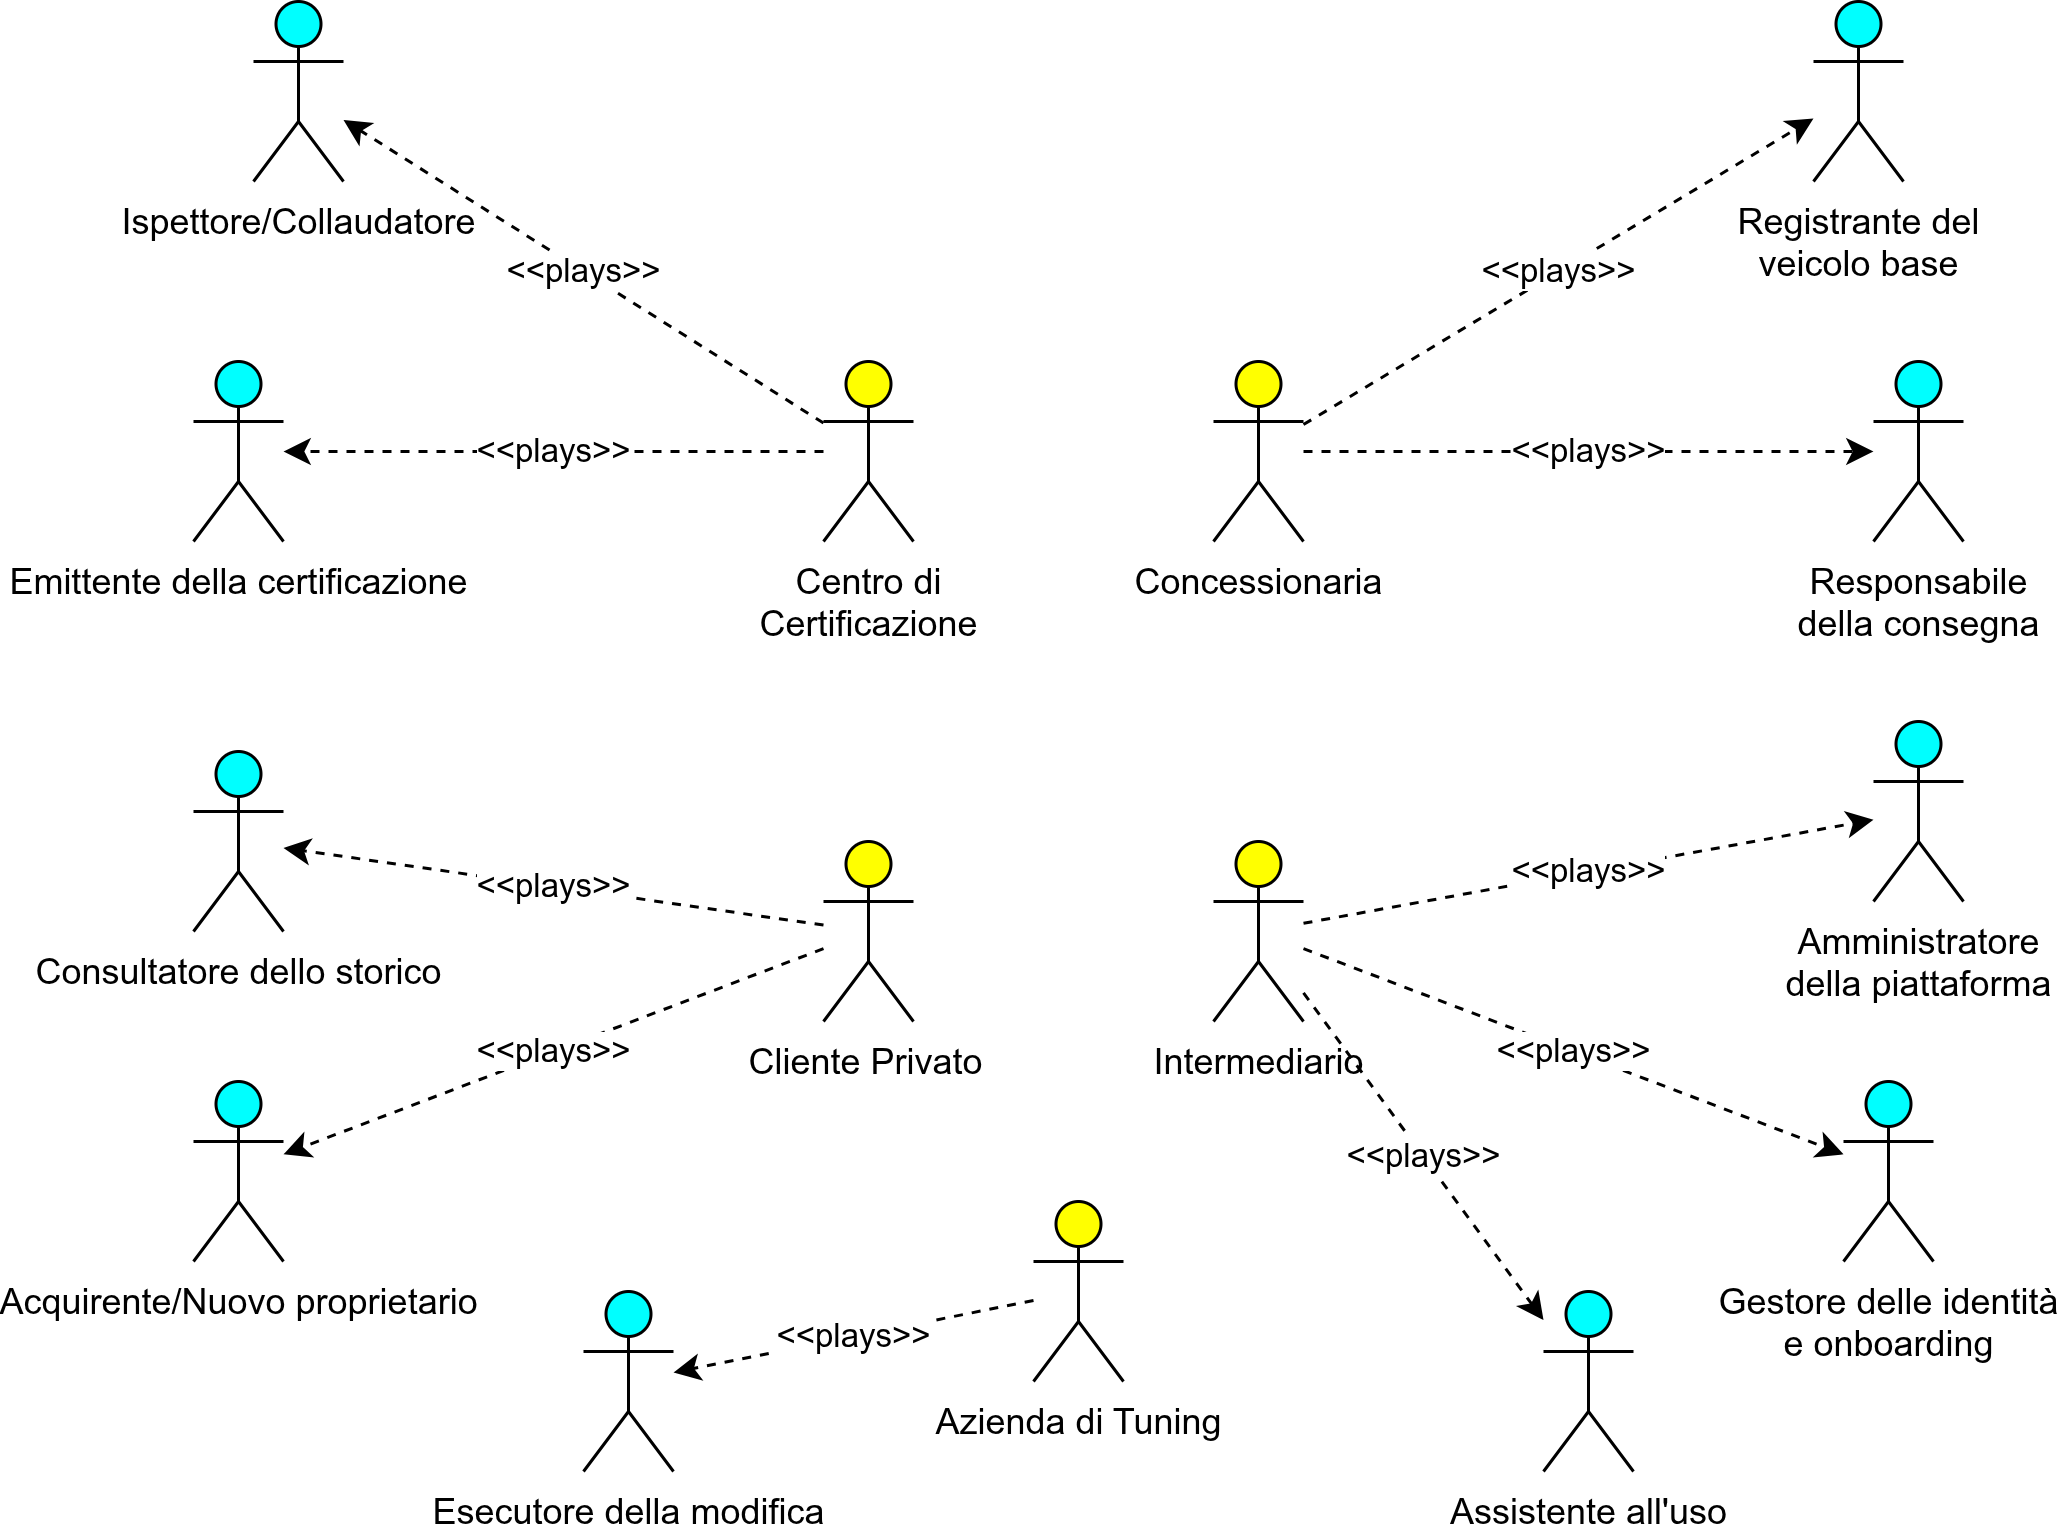
\includegraphics[width=\textwidth]{imgs/scenario/role_diagram.png}
    \caption{Role Diagram}
    \label{fig:role-diagram}
\end{figure}

La Figura~\ref{fig:goal-diagram} presenta i goal specifici associati a ciascun ruolo nello scenario. Coerentemente con l'impostazione adottata, a ogni ruolo corrisponde un unico obiettivo, che ne sintetizza la responsabilità all'interno del sistema.

\begin{figure}[H]
    \centering
    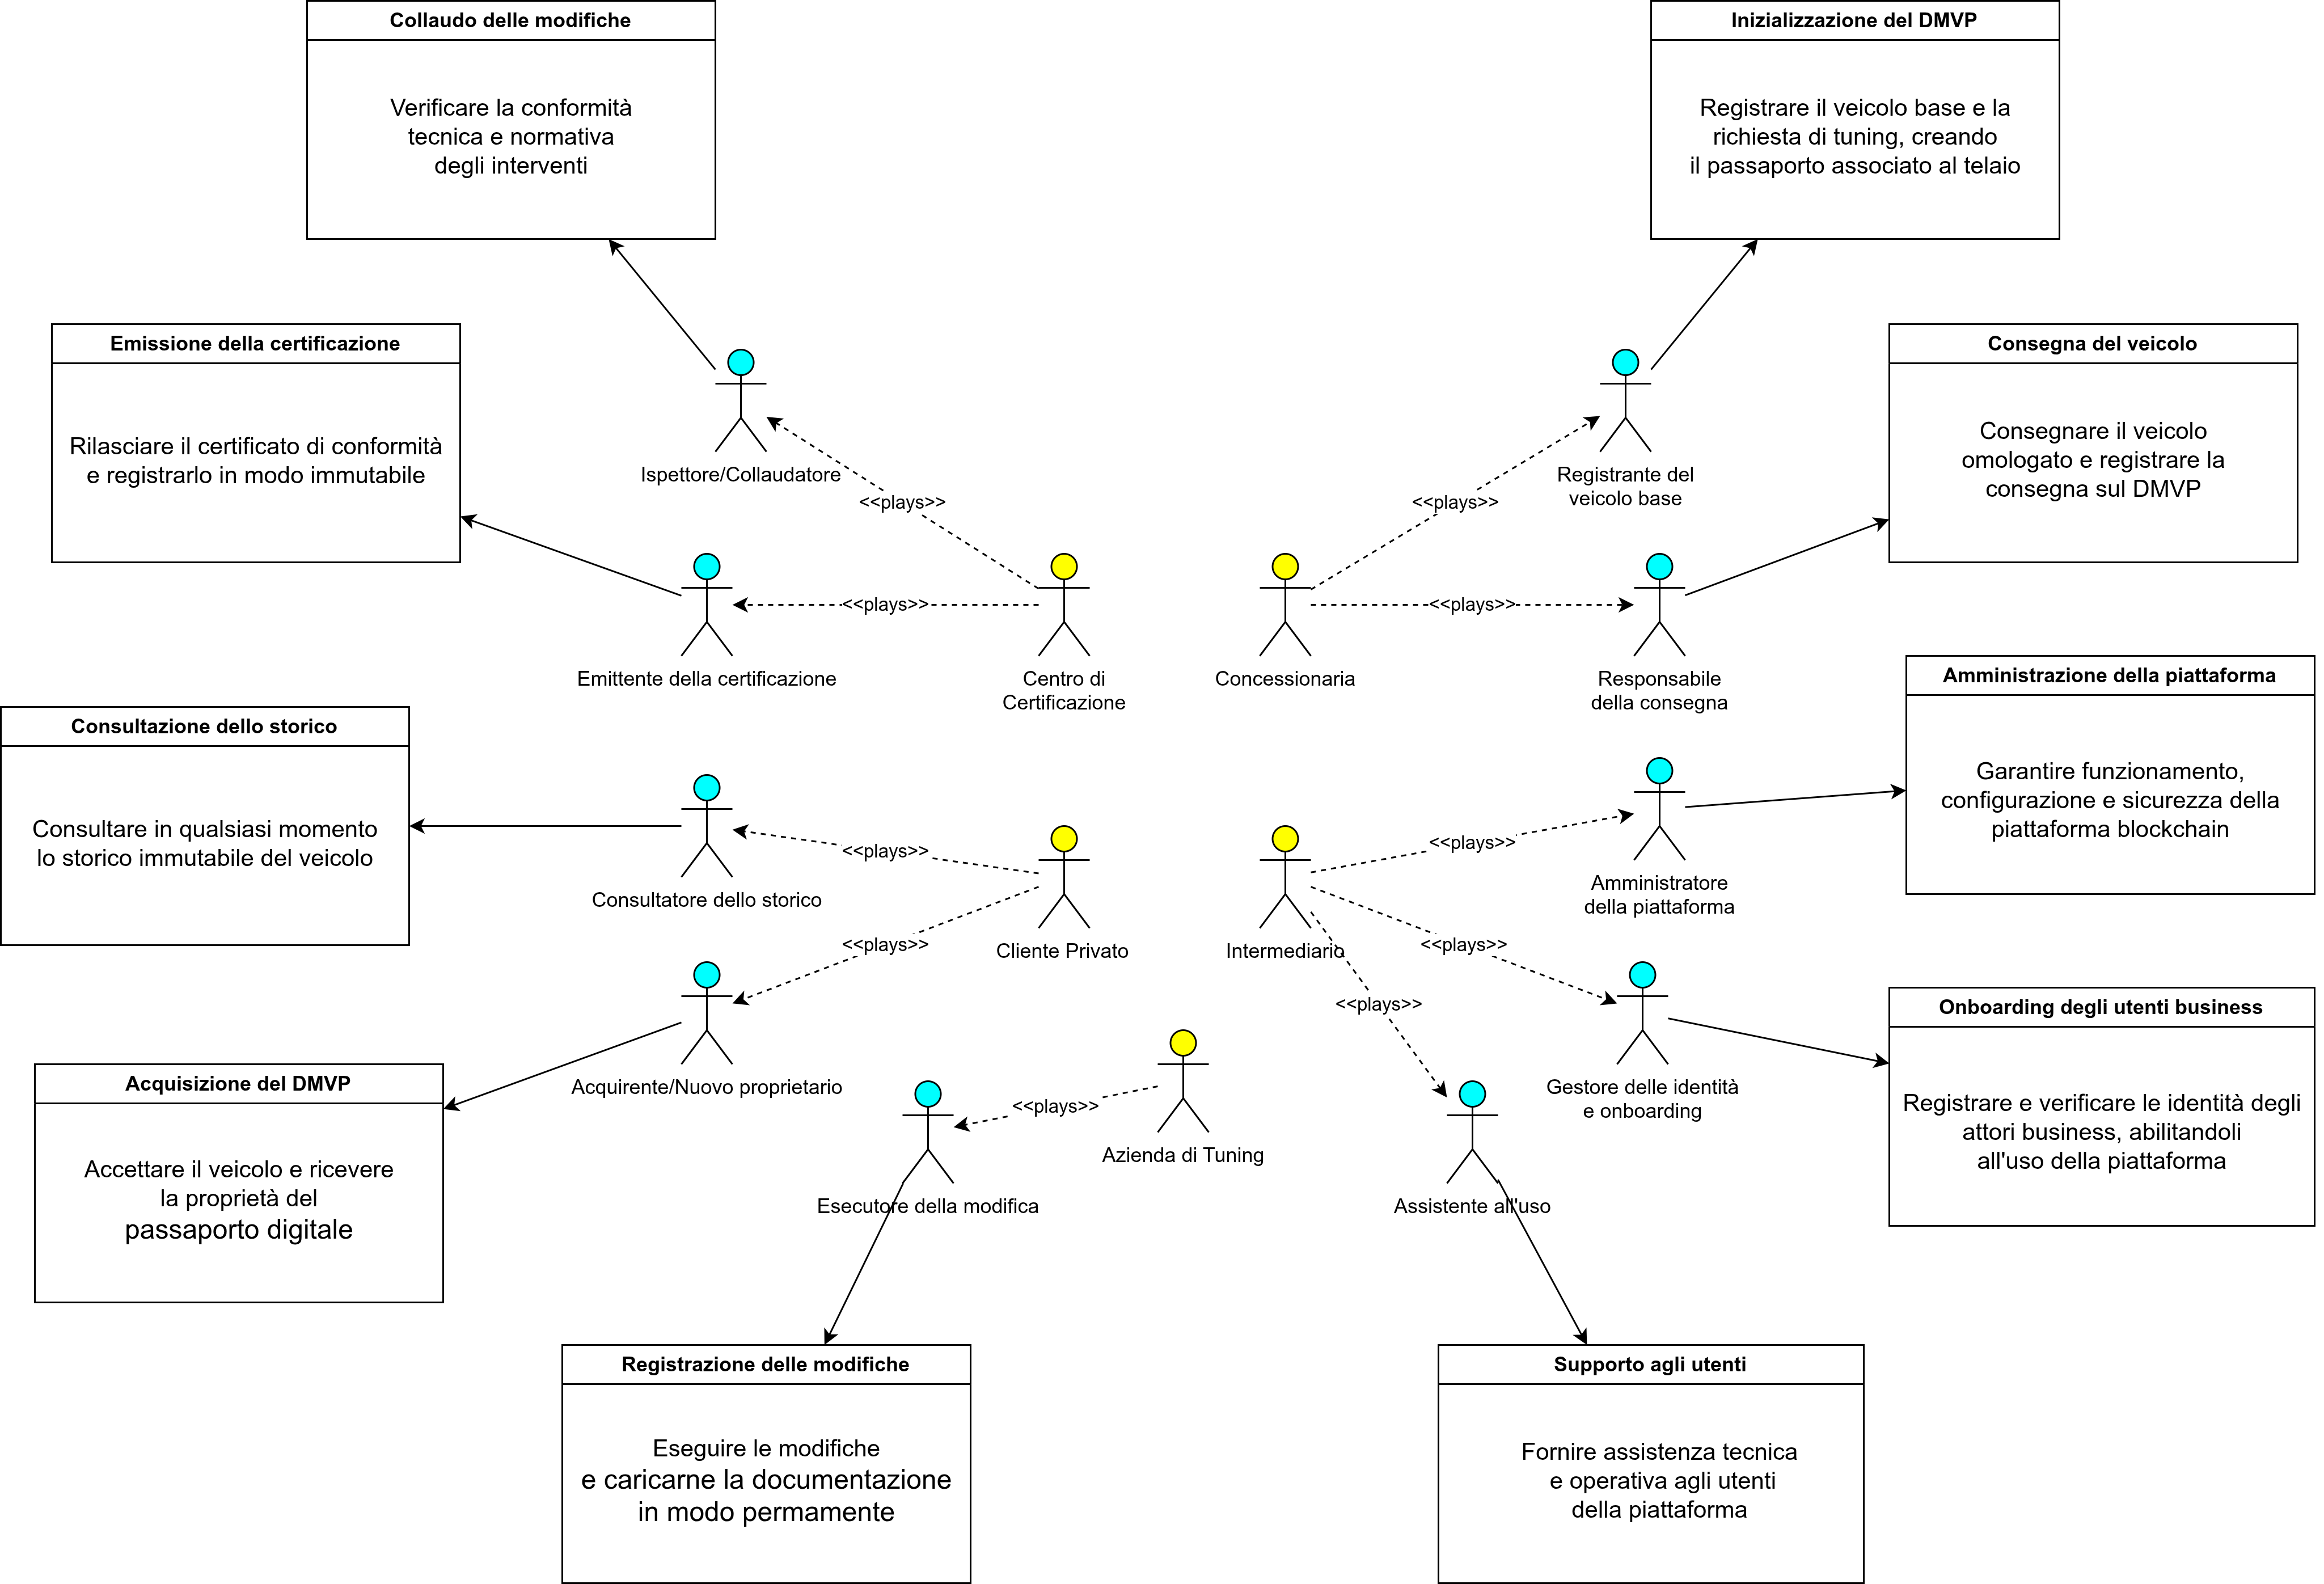
\includegraphics[width=\textwidth]{imgs/scenario/goal_diagram.png}
    \caption{Goal Diagram}
    \label{fig:goal-diagram}
\end{figure}

Se il Goal Diagram serve a isolare e definire i traguardi singoli di ogni ruolo, il \textbf{Goal Dependency Diagram} (Figura~\ref{fig:goal-dependency}) sposta l'attenzione sulla rete di relazioni e influenze che intercorrono tra di essi. L'obiettivo di questa rappresentazione è rendere esplicito come il raggiungimento di un fine possa agevolare (+) o, al contrario, ostacolare ($-$) le finalità degli altri ruoli coinvolti nel sistema.

\begin{figure}[H]
    \centering
    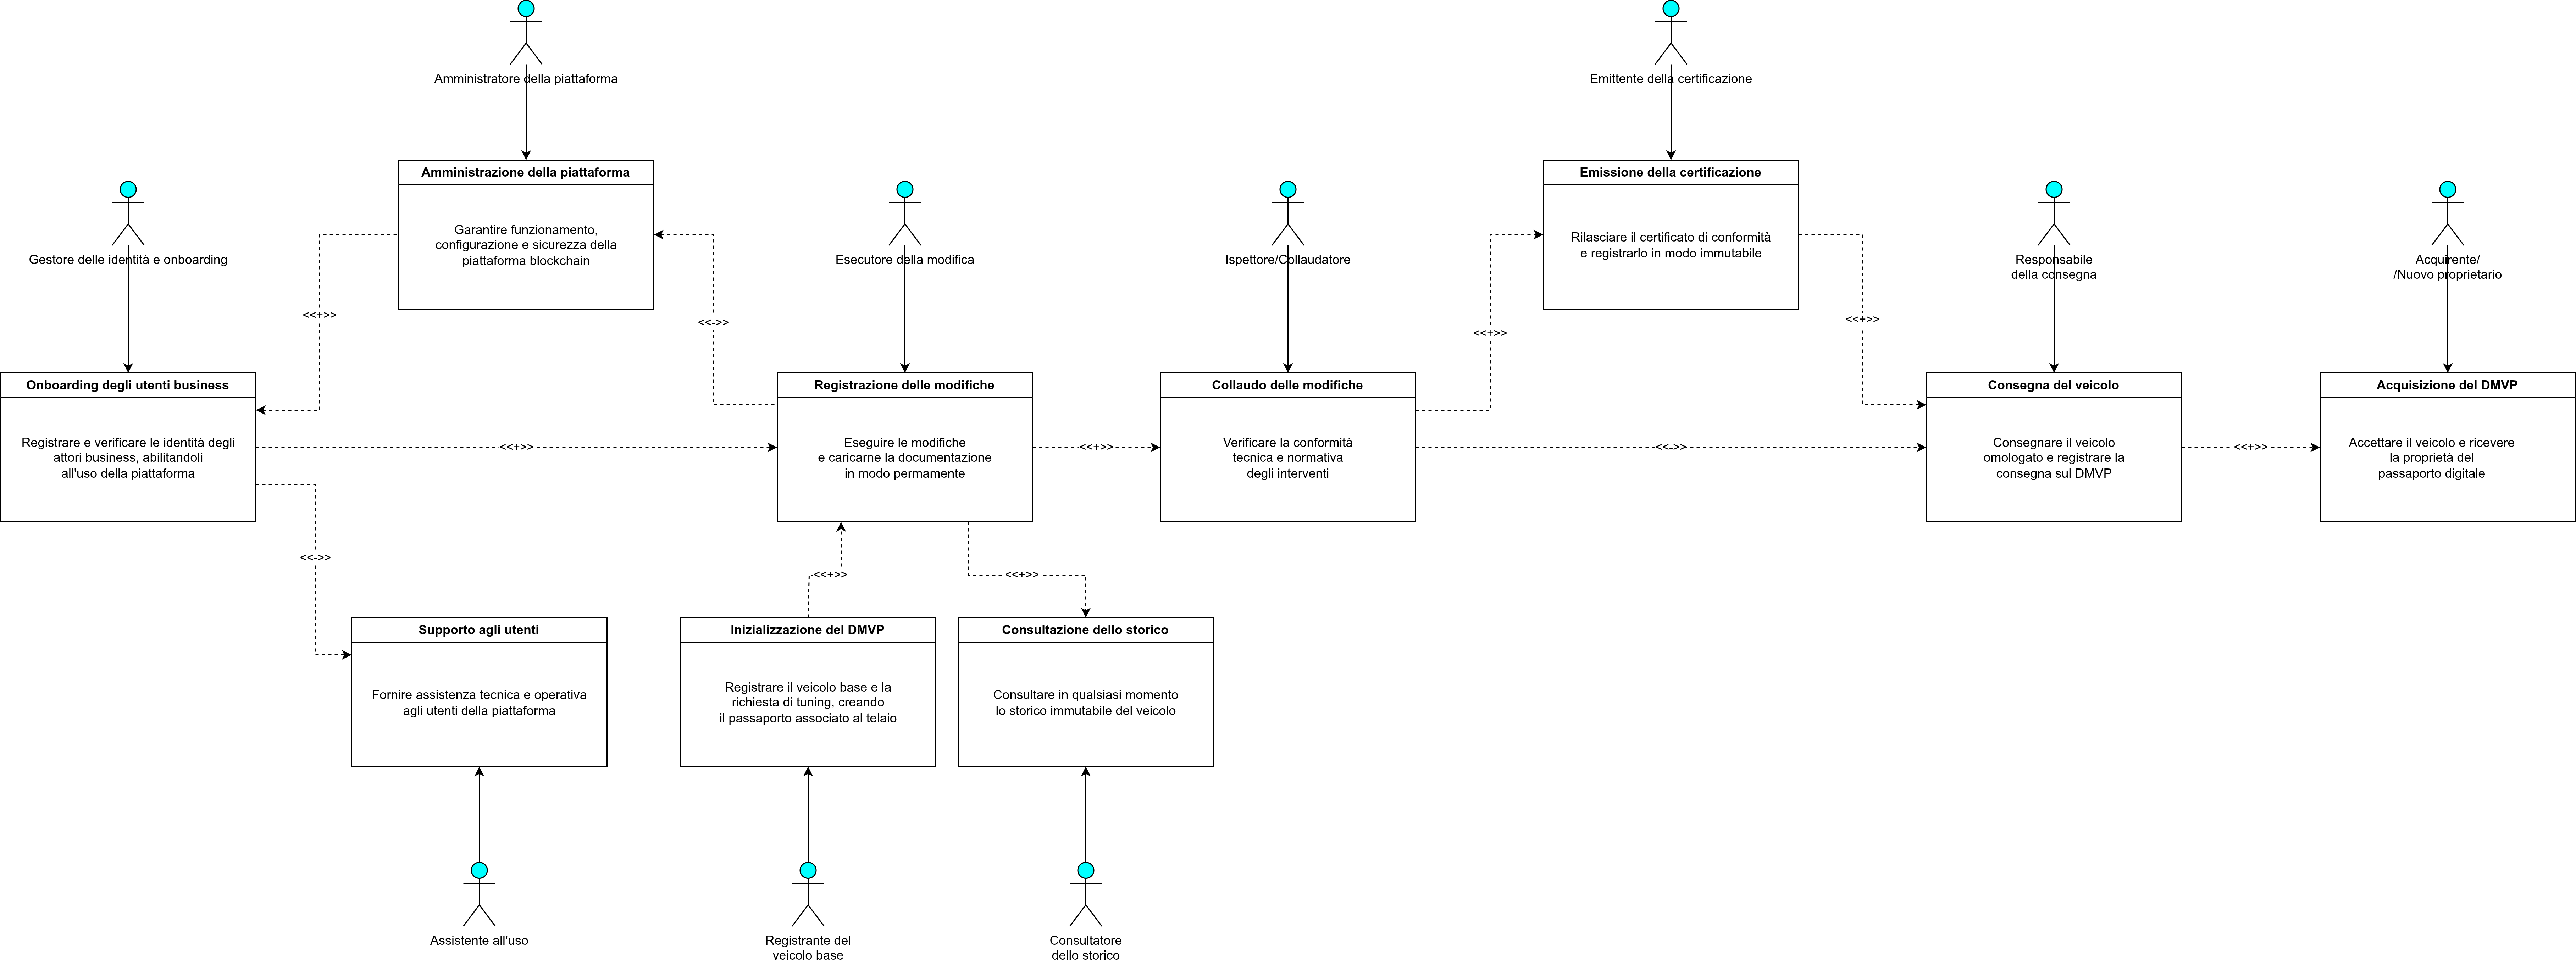
\includegraphics[width=\textwidth]{imgs/scenario/goal_dependency_diagram.png}
    \caption{Goal Dependency Diagram}
    \label{fig:goal-dependency}
\end{figure}

Vediamo nel dettaglio ogni dipendenza.

\subsection*{Contributes (+)}

\begin{itemize}
    \item \textbf{Amministrazione della piattaforma \quad$+$\quad Onboarding degli utenti business}\\
    Un'infrastruttura correttamente configurata e sicura costituisce il presupposto tecnico per poter abilitare nuovi attori: senza una rete permissioned funzionante e una Certification Authority operativa non sarebbe possibile emettere credenziali valide né ammettere organizzazioni al canale.

    \item \textbf{Onboarding degli utenti business \quad$+$\quad Registrazione delle modifiche}\\
    La verifica preventiva dell'identità degli attori garantisce che soltanto soggetti accreditati possano scrivere sul registro. Ne consegue che ogni lavorazione registrata è riconducibile in modo certo a un'azienda verificata, aumentando l'affidabilità del dato prodotto.

    \item \textbf{Inizializzazione del DMVP \quad$+$\quad Registrazione delle modifiche}\\
    L'esistenza del passaporto digitale associato al numero di telaio è la condizione necessaria affinché le modifiche possano esservi ancorate: senza l'istanza creata dalla Concessionaria, l'Azienda di Tuning non avrebbe alcun registro su cui operare.

    \item \textbf{Registrazione delle modifiche \quad$+$\quad Collaudo delle modifiche}\\
    Una documentazione tecnica completa, strutturata e immutabile consente al collaudatore di svolgere le verifiche in modo più rapido e oggettivo, evitando la ricostruzione manuale della storia degli interventi.

    \item \textbf{Collaudo delle modifiche \quad$+$\quad Emissione della certificazione}\\
    L'esito documentato delle verifiche tecniche e normative è il presupposto formale per il rilascio del certificato di conformità: senza collaudo non vi è alcuna base su cui fondare la certificazione.

    \item \textbf{Emissione della certificazione \quad$+$\quad Consegna del veicolo}\\
    La disponibilità del certificato registrato in modo immutabile abilita la Concessionaria ad avviare la procedura di consegna, potendo dimostrare la piena regolarità del veicolo modificato.

    \item \textbf{Consegna del veicolo \quad$+$\quad Acquisizione del DMVP}\\
    La consegna formale del veicolo omologato è ciò che innesca il trasferimento della proprietà del passaporto digitale all'account del Cliente Privato, completando il ciclo di tracciabilità.

    \item \textbf{Registrazione delle modifiche \quad$+$\quad Consultazione dello storico}\\
    Quanto più le lavorazioni vengono registrate in modo puntuale e dettagliato, tanto più lo storico consultabile dal Cliente Privato risulta completo e significativo ai fini della verifica di autenticità e della valorizzazione del veicolo.
\end{itemize}

\subsection*{Hinders ($-$)}

\begin{itemize}
    \item \textbf{Registrazione delle modifiche \quad$-$\quad Amministrazione della piattaforma}\\
    Il volume crescente di documentazione caricata e di ancoraggi sulla catena appesantisce la gestione dell'infrastruttura, incrementando i requisiti di storage, il carico sui nodi e l'onere di monitoraggio a carico dell'Intermediario.

    \item \textbf{Onboarding degli utenti business \quad$-$\quad Supporto agli utenti}\\
    L'ampliamento della base di attori abilitati genera un corrispondente aumento delle richieste di assistenza e di formazione, rendendo più difficile mantenere gli stessi livelli di servizio a parità di risorse dedicate al supporto.

    \item \textbf{Collaudo delle modifiche \quad$-$\quad Consegna del veicolo}\\
    Il rigore delle verifiche tecniche e normative, pur necessario a garantire la conformità, allunga i tempi complessivi del processo e può ritardare la consegna del veicolo al cliente, soprattutto qualora il collaudo dia esito negativo e imponga interventi correttivi.
\end{itemize}

\section{Modello di Business dell'Idea Progettuale in Canvas}

\subsection{Schema del Modello di Business dell'Idea Progettuale}

La Figura~\ref{fig:canvas} illustra il modello di business dell'idea progettuale, realizzato con il formalismo Canvas. Il modello è costruito attorno all'individuazione dell'\textbf{Intermediario} quale cliente primario della piattaforma e organizza il valore offerto per segmento, in modo che a ciascuno stakeholder corrisponda la proposta di valore che ne motiva l'adesione.

\begin{figure}[H]
    \centering
    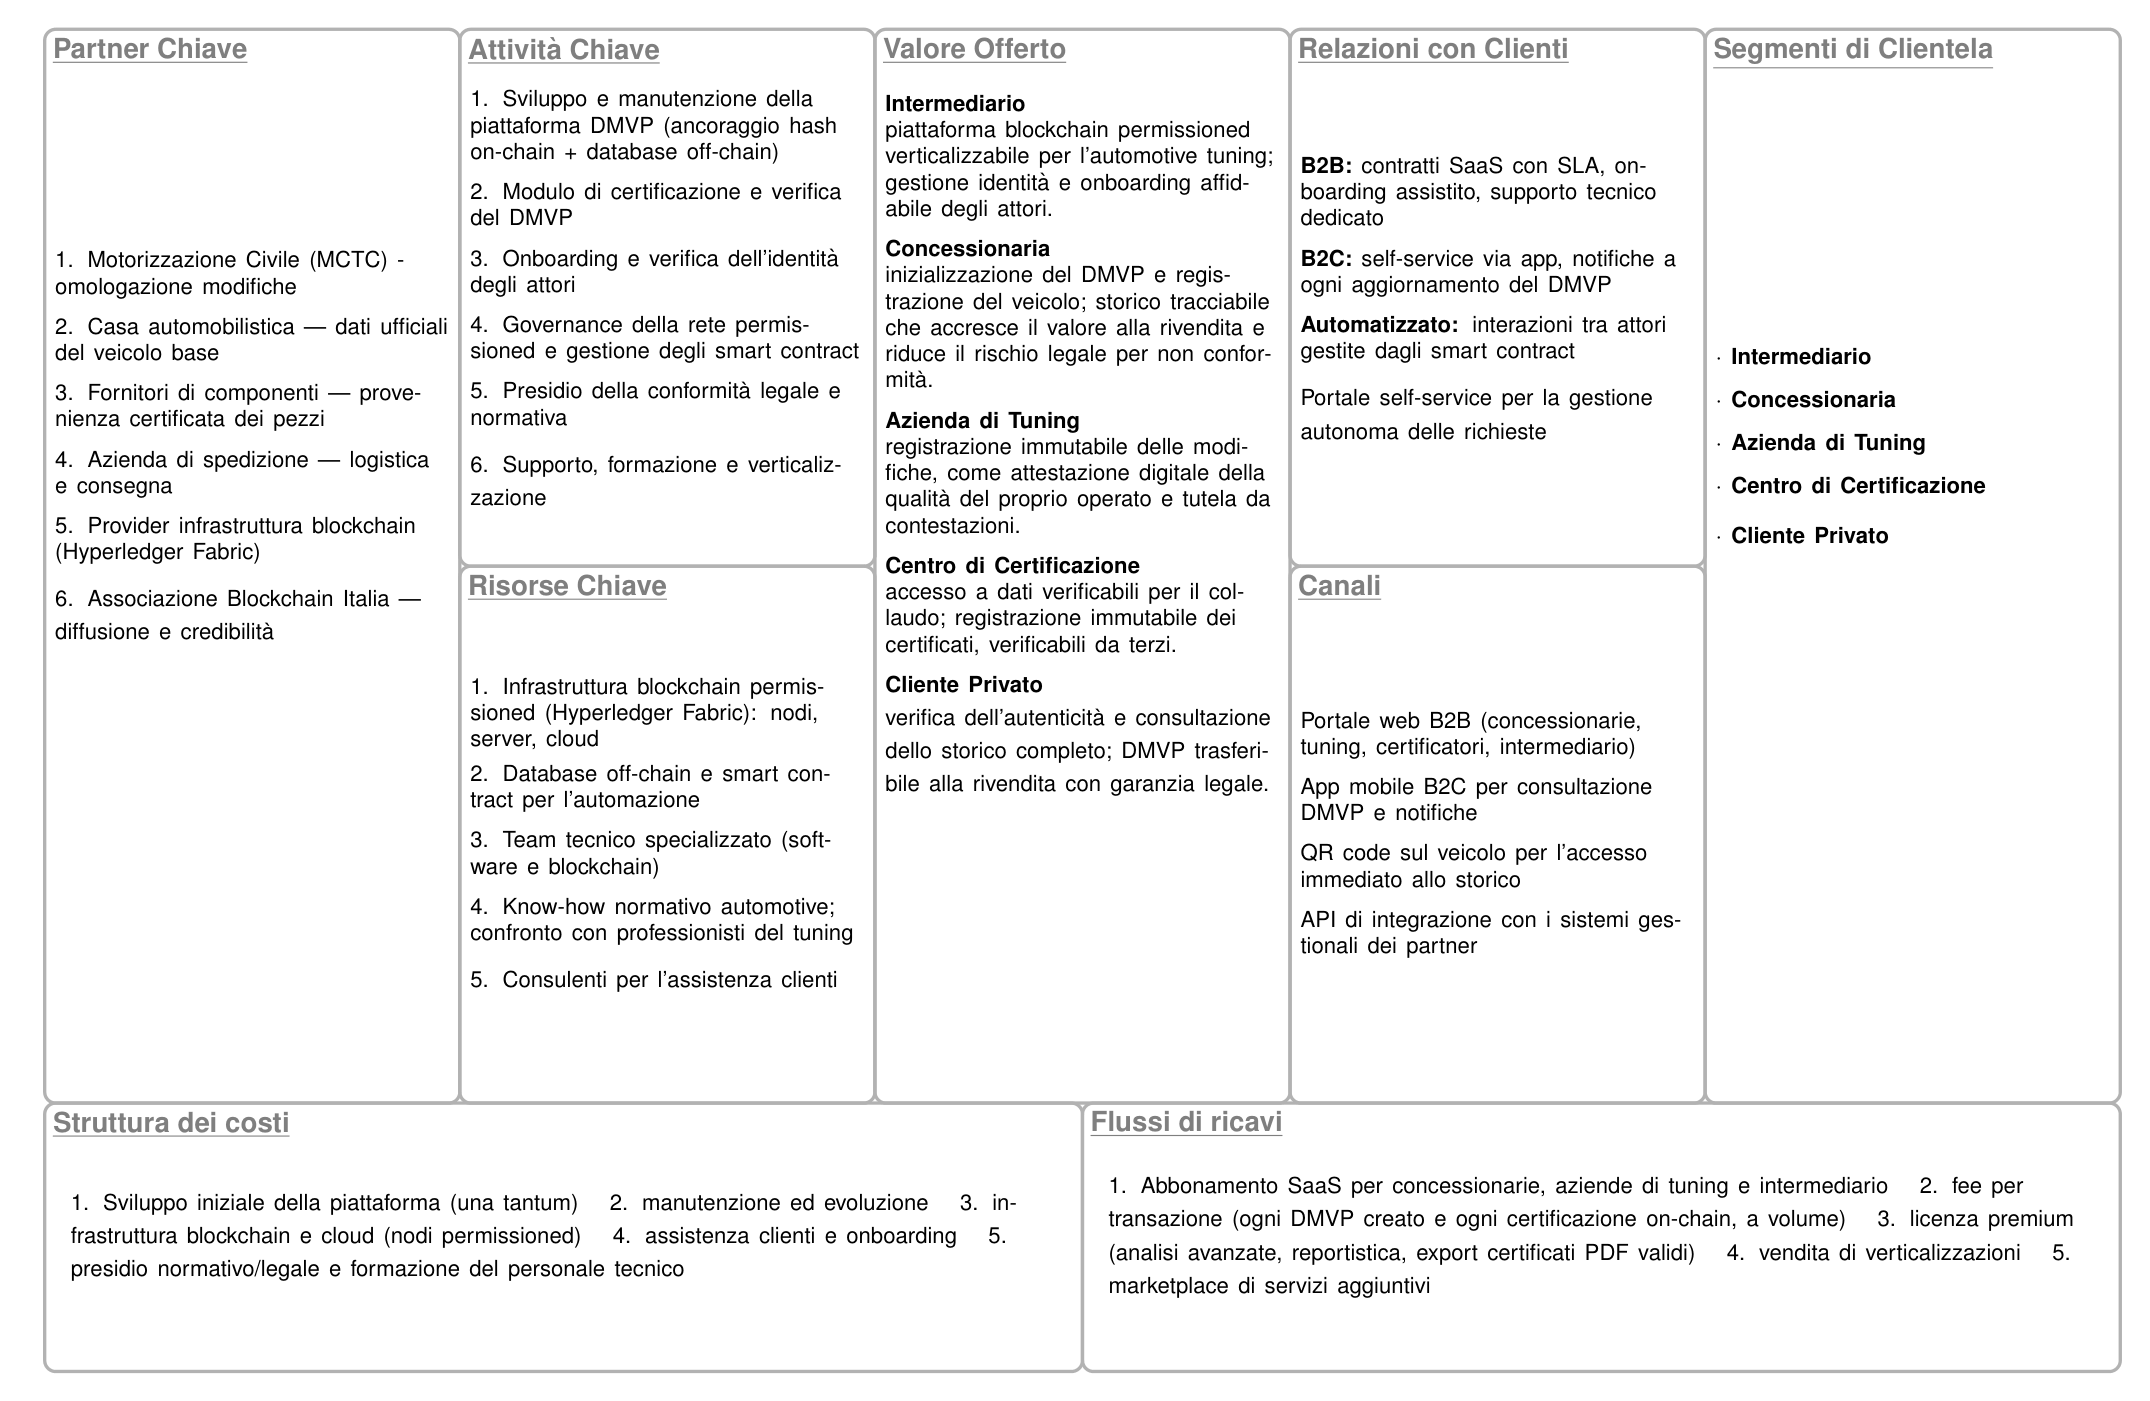
\includegraphics[width=\textwidth]{imgs/scenario/business_model_canvas.png}
    \caption{Modello di Business in Canvas}
    \label{fig:canvas}
\end{figure}

\subsection{Descrizione in dettaglio del Modello di Business}

\subsubsection*{Partner Chiave}

\begin{itemize}
    \item \textbf{Motorizzazione Civile (MCTC)}: ente competente per l'omologazione delle modifiche apportate ai veicoli. Rappresenta il partner istituzionale di riferimento, la cui collaborazione è determinante per il riconoscimento formale del DMVP.
    \item \textbf{Casa automobilistica}: fornisce i dati ufficiali del veicolo base, necessari all'inizializzazione del passaporto digitale.
    \item \textbf{Fornitori di componenti}: attestano la provenienza certificata dei pezzi installati, consentendo di estendere la tracciabilità anche a monte della lavorazione.
    \item \textbf{Azienda di spedizione}: gestisce la logistica e la consegna del veicolo, fase che il DMVP registra come passaggio di responsabilità.
    \item \textbf{Provider dell'infrastruttura blockchain}: fornisce la tecnologia su cui poggia la rete permissioned.
    \item \textbf{Associazione Blockchain Italia}: organizzazione no-profit attiva nella promozione delle tecnologie DLT, partner strategico per il posizionamento istituzionale della soluzione e la sensibilizzazione degli stakeholder.
\end{itemize}

\subsubsection*{Attività Chiave}

Le attività chiave comprendono lo sviluppo e la manutenzione della piattaforma DMVP, nella duplice componente di ancoraggio degli hash on-chain e di gestione del database off-chain; lo sviluppo del modulo di certificazione e verifica del passaporto; l'onboarding e la verifica dell'identità degli attori; la governance della rete permissioned e la gestione degli smart contract; il presidio della conformità legale e normativa, particolarmente critico in un settore regolamentato come quello dell'omologazione veicolare; e infine le attività di supporto, formazione e verticalizzazione della piattaforma.

\subsubsection*{Risorse Chiave}

Le risorse chiave sono costituite dall'infrastruttura blockchain permissioned, comprensiva di nodi, server e servizi cloud; dal database off-chain e dagli smart contract per l'automazione dei processi; dal team tecnico specializzato in sviluppo software e tecnologie a registro distribuito; dal know-how normativo in ambito automotive, alimentato dal confronto con i professionisti del settore; e dai consulenti a supporto dell'assistenza clienti.

\subsubsection*{Valore Offerto}

Il valore offerto è articolato per segmento, in modo che ciascuna proposta risulti direttamente riconducibile ai casi d'uso descritti nel capitolo seguente:

\begin{itemize}
    \item \textbf{Intermediario}: piattaforma blockchain permissioned verticalizzabile per la filiera dell'automotive tuning, con gestione affidabile delle identità e dell'onboarding degli attori.
    \item \textbf{Concessionaria}: inizializzazione del DMVP e registrazione del veicolo; storico tracciabile che ne accresce il valore alla rivendita e riduce il rischio legale per non conformità.
    \item \textbf{Azienda di Tuning}: registrazione immutabile delle modifiche eseguite, quale attestazione digitale della qualità del proprio operato e tutela da contestazioni.
    \item \textbf{Centro di Certificazione}: accesso a dati verificabili per il collaudo e registrazione immutabile dei certificati emessi, controllabili da terzi.
    \item \textbf{Cliente Privato}: verifica dell'autenticità e consultazione dello storico completo del veicolo; passaporto digitale trasferibile alla rivendita.
\end{itemize}

\subsubsection*{Relazioni con i Clienti}

La relazione con i clienti si articola su tre modalità. Sul versante \textbf{B2B} si adottano contratti SaaS con livelli di servizio definiti, onboarding assistito e supporto tecnico dedicato, coerentemente con la natura tecnica dell'infrastruttura. Sul versante \textbf{B2C} la relazione è di tipo self-service attraverso l'applicazione mobile, con notifiche automatiche a ogni aggiornamento del DMVP. Una componente \textbf{automatizzata} è infine garantita dagli smart contract, che gestiscono le interazioni tra attori senza necessità di coordinamento manuale. A queste si affianca un portale self-service per la gestione autonoma delle richieste.

\subsubsection*{Canali}

La distribuzione avviene attraverso un portale web B2B destinato a concessionarie, aziende di tuning, centri di certificazione e intermediario; un'applicazione mobile B2C per la consultazione del DMVP e la ricezione delle notifiche; un QR code applicato al veicolo, che consente l'accesso immediato allo storico anche a un potenziale acquirente; e infine API di integrazione con i sistemi gestionali dei partner.

\subsubsection*{Segmenti di Clientela}

I segmenti di clientela coincidono con gli stakeholder dello scenario specifico: Intermediario, Concessionaria, Azienda di Tuning, Centro di Certificazione e Cliente Privato. Tra questi, l'\textbf{Intermediario} riveste il ruolo di cliente primario, in quanto soggetto che acquisisce la piattaforma e ne cura la verticalizzazione presso gli altri attori della filiera.

\subsubsection*{Struttura dei Costi}

La struttura dei costi comprende lo sviluppo iniziale della piattaforma, sostenuto una tantum; la manutenzione e l'evoluzione del sistema; l'infrastruttura blockchain e cloud, con particolare riferimento all'esercizio dei nodi permissioned; l'assistenza clienti e l'onboarding; e infine il presidio normativo e legale, unitamente alla formazione del personale tecnico. L'analisi economica dettagliata di tali voci è sviluppata nel Business Plan (Capitolo~7).

\subsubsection*{Flussi di Ricavi}

I flussi di ricavo previsti sono di natura prevalentemente B2B e comprendono l'abbonamento SaaS per concessionarie, aziende di tuning e intermediario; una fee per transazione proporzionale al volume di DMVP creati e di certificazioni registrate on-chain; una licenza premium per analisi avanzate, reportistica ed esportazione di certificati in formato legalmente valido; la vendita di verticalizzazioni della piattaforma; e un marketplace di servizi aggiuntivi.
\chapter{Idea Progettuale: Modello degli Use Case e dei Processi}

In questo capitolo vengono presentati i principali use-case di \textit{Tuning Ledger}, la piattaforma per la gestione del \textit{Digital Modified Vehicle Passport} (DMVP), con l'obiettivo di descrivere in modo formale le interazioni tra gli attori e il sistema. Successivamente, i processi principali vengono modellati tramite diagrammi BPMN, al fine di rappresentare il flusso operativo delle attività di registrazione, esecuzione, certificazione e consegna del veicolo modificato.

\section{Modellazione degli Use-Case principali in GOREM}

La piattaforma, al fine di soddisfare tutte le richieste degli attori coinvolti, considera i casi d'uso di seguito riportati, organizzati per ciascuno degli stakeholder individuati nello scenario specifico. Coerentemente con la modellazione dei ruoli presentata nel Capitolo~3, a ogni ruolo corrisponde uno use-case: ciascuno stakeholder \textit{gioca} (\texttt{<<plays>>}) uno o più ruoli, e da ciascun ruolo discende l'operazione di cui esso è responsabile all'interno del sistema.

In tutti i diagrammi, le azioni che comportano una scrittura sul registro distribuito sono modellate come use-case inclusi (\texttt{<<include>>}) e vedono l'\textbf{Intermediario} come attore secondario, in quanto gestore della piattaforma e unico soggetto abilitato a operare sull'infrastruttura blockchain.

\subsection*{Concessionaria}

La Concessionaria gioca due ruoli, ai quali corrispondono altrettante operazioni (Figura~\ref{fig:uc-concessionaria}):

\begin{enumerate}
    \item \textit{Registrante del veicolo base}, che inserisce sulla piattaforma i dati identificativi del veicolo originale forniti dalla Casa Automobilistica e le modifiche commissionate dal Cliente Privato. L'operazione include l'inizializzazione del DMVP, ossia la creazione dell'istanza del passaporto digitale associata univocamente al numero di telaio.
    \item \textit{Responsabile della consegna}, che avvia la procedura di consegna del veicolo omologato al termine dell'iter tecnico. L'operazione include la registrazione della consegna sul DMVP.
\end{enumerate}

\begin{figure}[H]
    \centering
    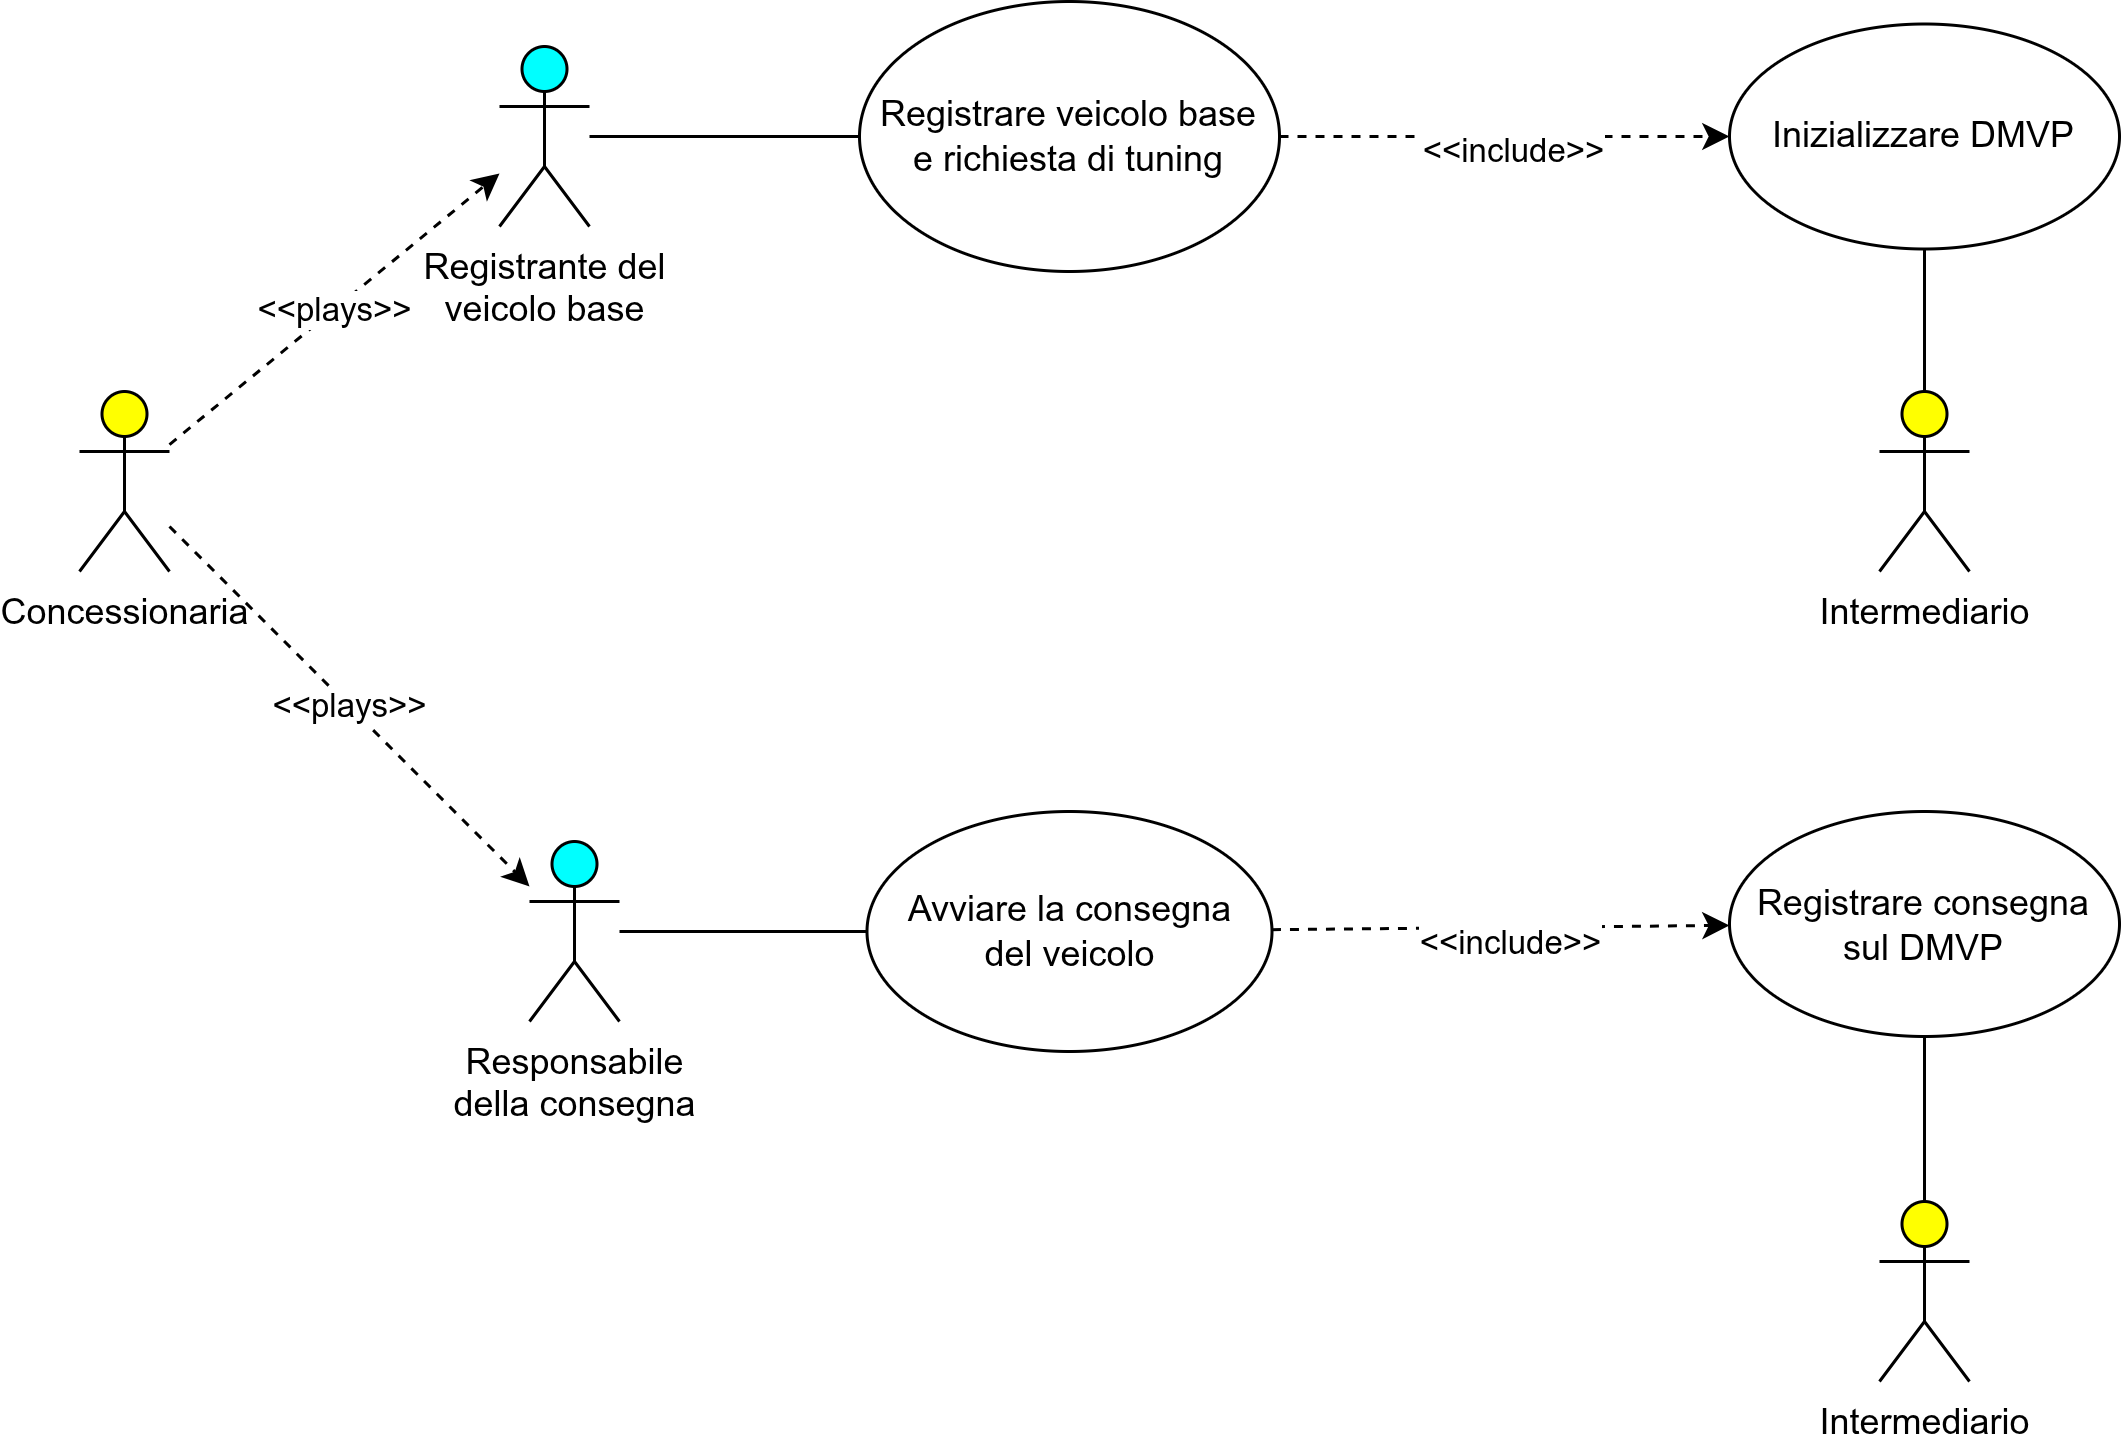
\includegraphics[width=\textwidth]{imgs/usecase/01_concessionaria.png}
    \caption{Use-Case Concessionaria}
    \label{fig:uc-concessionaria}
\end{figure}

\subsection*{Azienda di Tuning}

L'Azienda di Tuning gioca il ruolo di \textit{Esecutore delle modifiche}, responsabile della registrazione sul DMVP delle lavorazioni effettivamente eseguite sul veicolo. Tale operazione si articola in tre azioni incluse (Figura~\ref{fig:uc-tuning}):

\begin{itemize}
    \item la compilazione della \textbf{scheda tecnica modificata}, contenente le specifiche degli interventi e i codici seriali dei componenti installati;
    \item l'acquisizione delle \textbf{prove multimediali} a corredo delle lavorazioni, quali fotografie e documentazione tecnica;
    \item l'\textbf{ancoraggio dell'hash} dei dati registrati sulla blockchain, eseguito tramite l'Intermediario.
\end{itemize}

Quest'ultimo punto rende esplicita l'architettura ibrida della soluzione: la documentazione voluminosa risiede nel database off-chain, mentre sulla catena viene registrata soltanto l'impronta crittografica che ne garantisce l'integrità.

\begin{figure}[H]
    \centering
    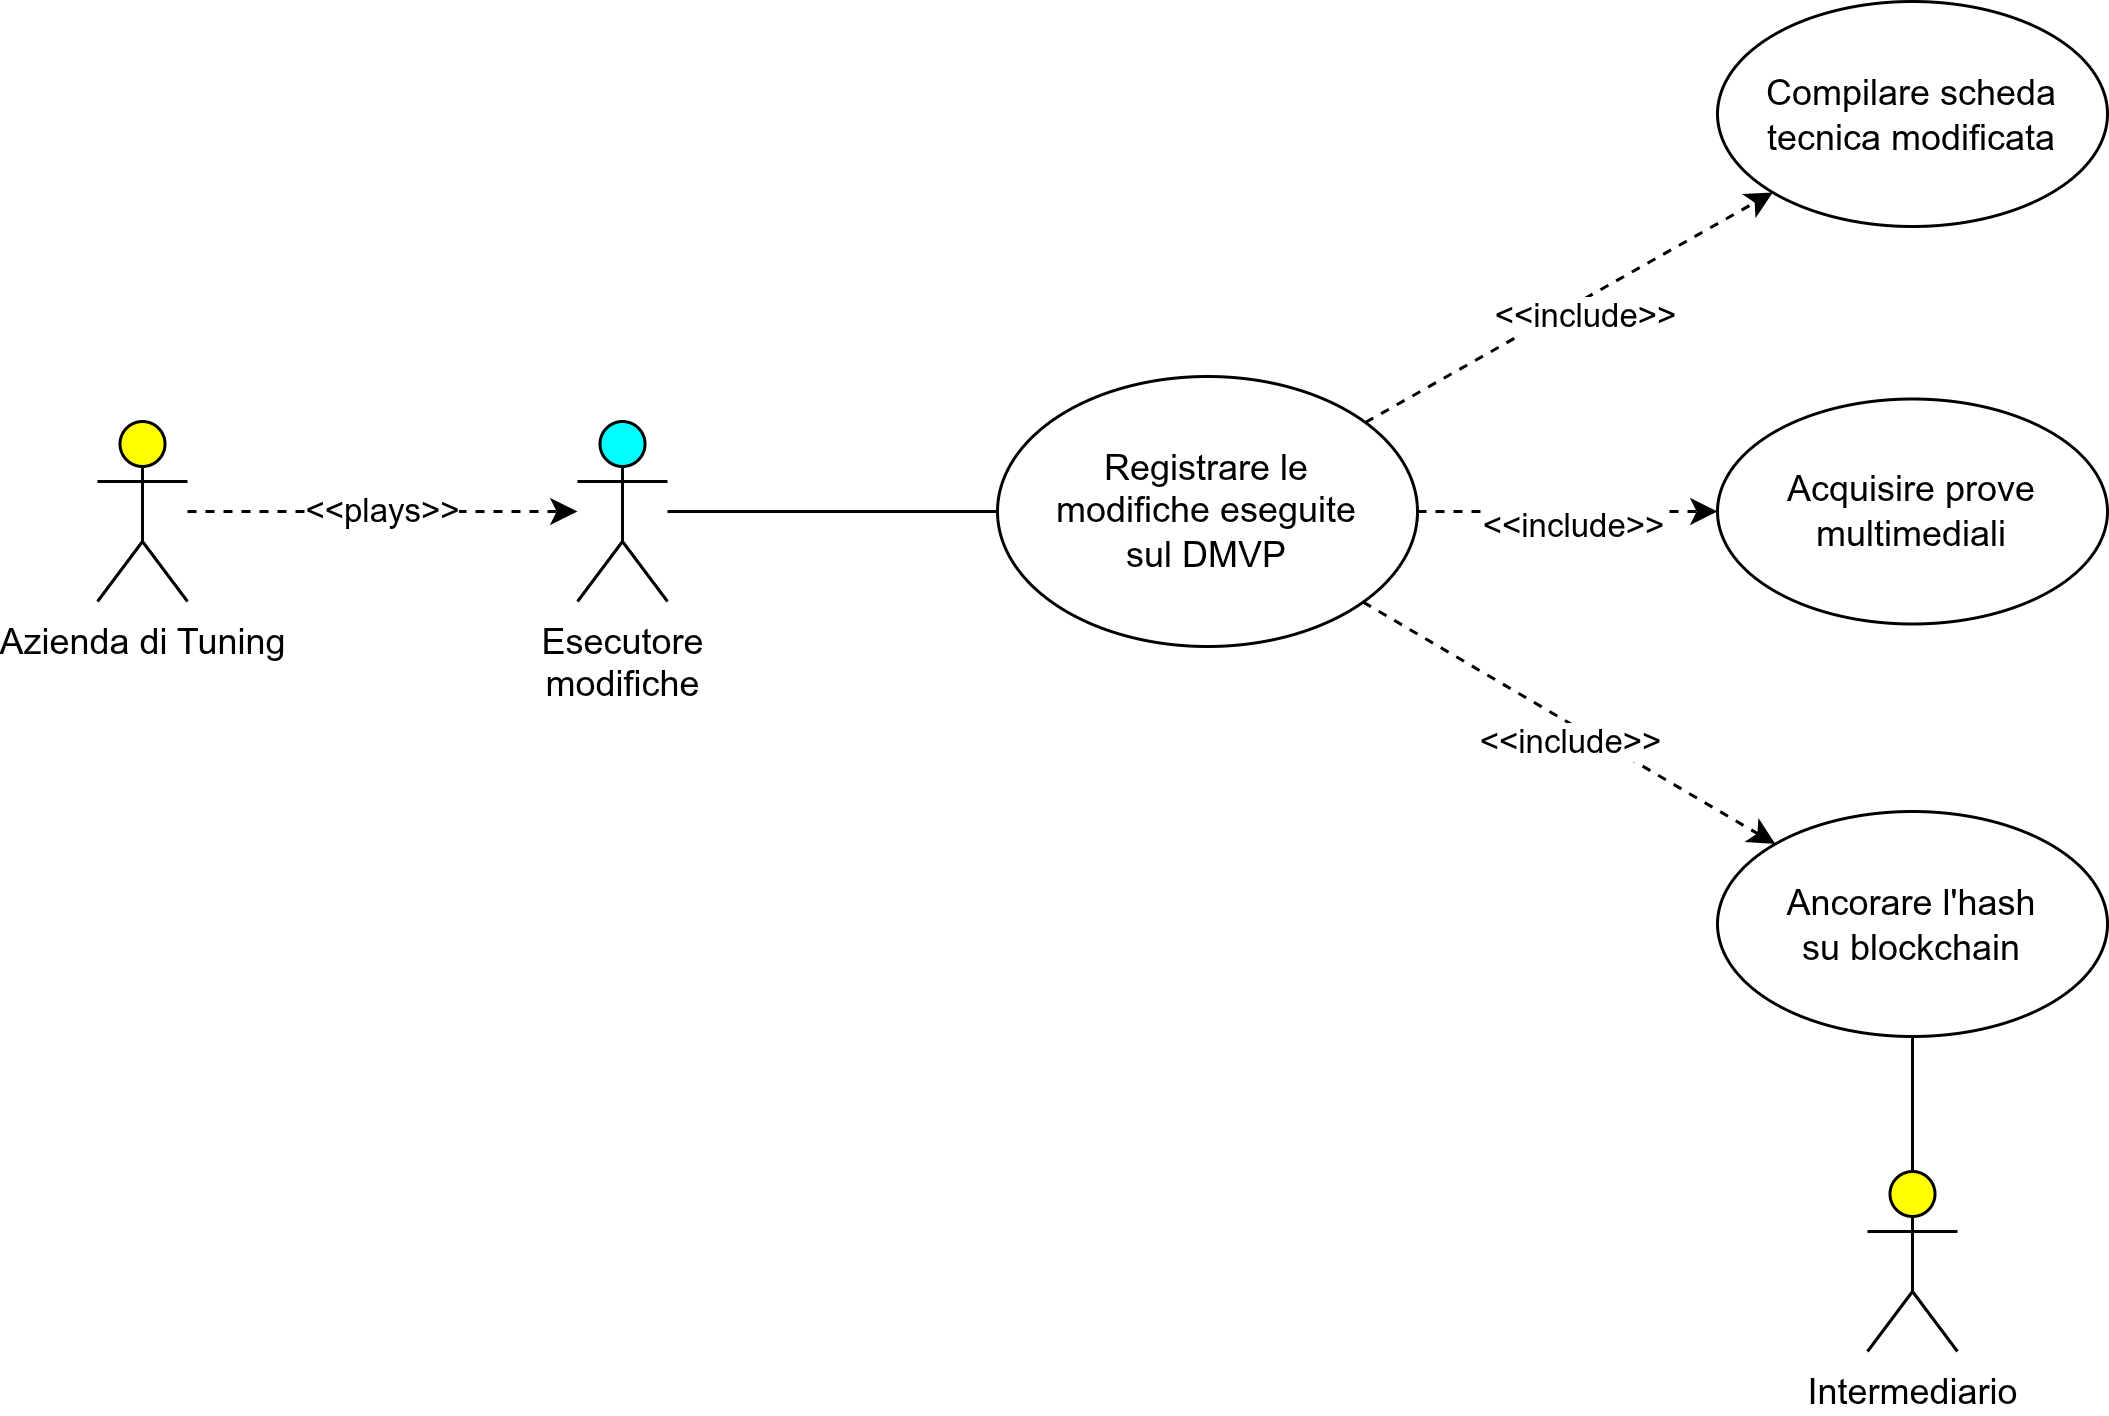
\includegraphics[width=\textwidth]{imgs/usecase/02_azienda_di_tuning.png}
    \caption{Use-Case Azienda di Tuning}
    \label{fig:uc-tuning}
\end{figure}

\subsection*{Centro di Certificazione}

Il Centro di Certificazione gioca due ruoli distinti (Figura~\ref{fig:uc-certificazione}), corrispondenti alle due fasi logicamente separate della sua attività:

\begin{enumerate}
    \item \textit{Ispettore/Collaudatore}, che esegue le verifiche tecniche e normative sulle modifiche apportate. L'operazione include la consultazione dello storico del DMVP, necessaria per accertare che tutte le fasi precedenti siano state svolte correttamente. A tale use-case è associata, come flusso alternativo, la \textbf{segnalazione di non conformità} (\texttt{<<extend>>}), attivata nel caso in cui il collaudo dia esito negativo.
    \item \textit{Emittente della certificazione}, che rilascia il certificato digitale di conformità al superamento del collaudo. L'operazione include la registrazione del certificato sulla blockchain, con conseguente aggiornamento dello stato del DMVP.
\end{enumerate}

\begin{figure}[H]
    \centering
    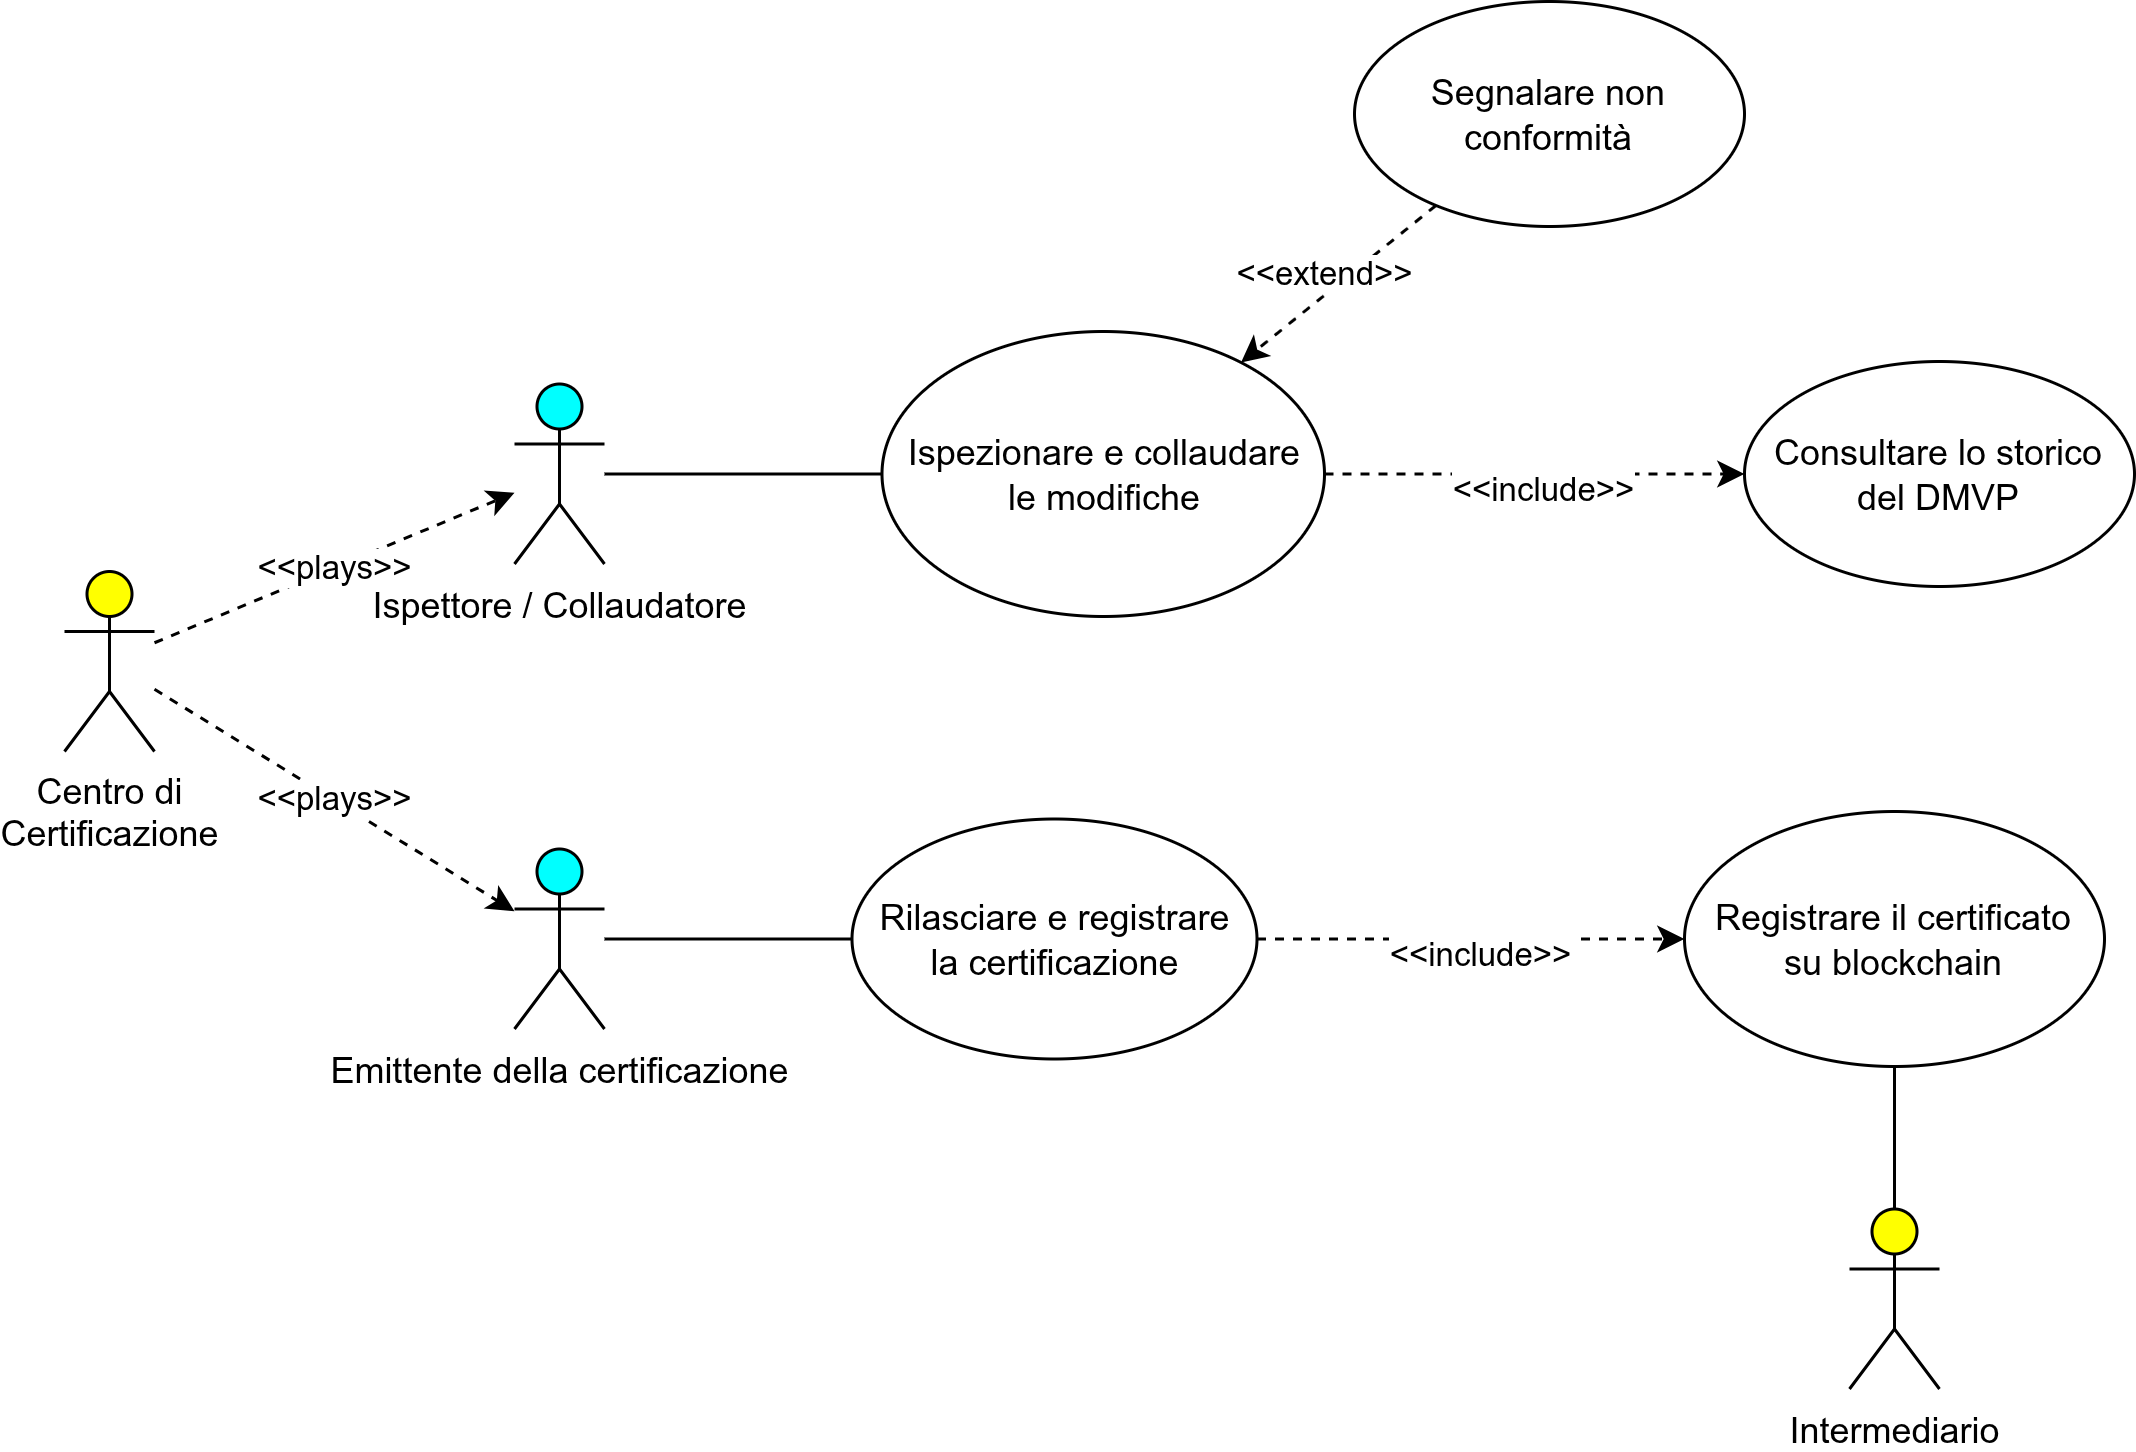
\includegraphics[width=\textwidth]{imgs/usecase/03_centro_di_certificazione.png}
    \caption{Use-Case Centro di Certificazione}
    \label{fig:uc-certificazione}
\end{figure}

\subsection*{Cliente Privato}

Il Cliente Privato gioca due ruoli (Figura~\ref{fig:uc-cliente}):

\begin{enumerate}
    \item \textit{Consultatore dello storico}, che accede in sola lettura al registro immutabile del veicolo per verificarne l'autenticità e ricostruirne la storia completa, sia prima dell'accettazione sia in qualunque momento successivo.
    \item \textit{Acquirente/nuovo proprietario}, che accetta il veicolo al termine della consegna e ne riceve il passaporto digitale. L'operazione include il trasferimento della proprietà del DMVP, registrato sulla blockchain tramite l'Intermediario.
\end{enumerate}

\begin{figure}[H]
    \centering
    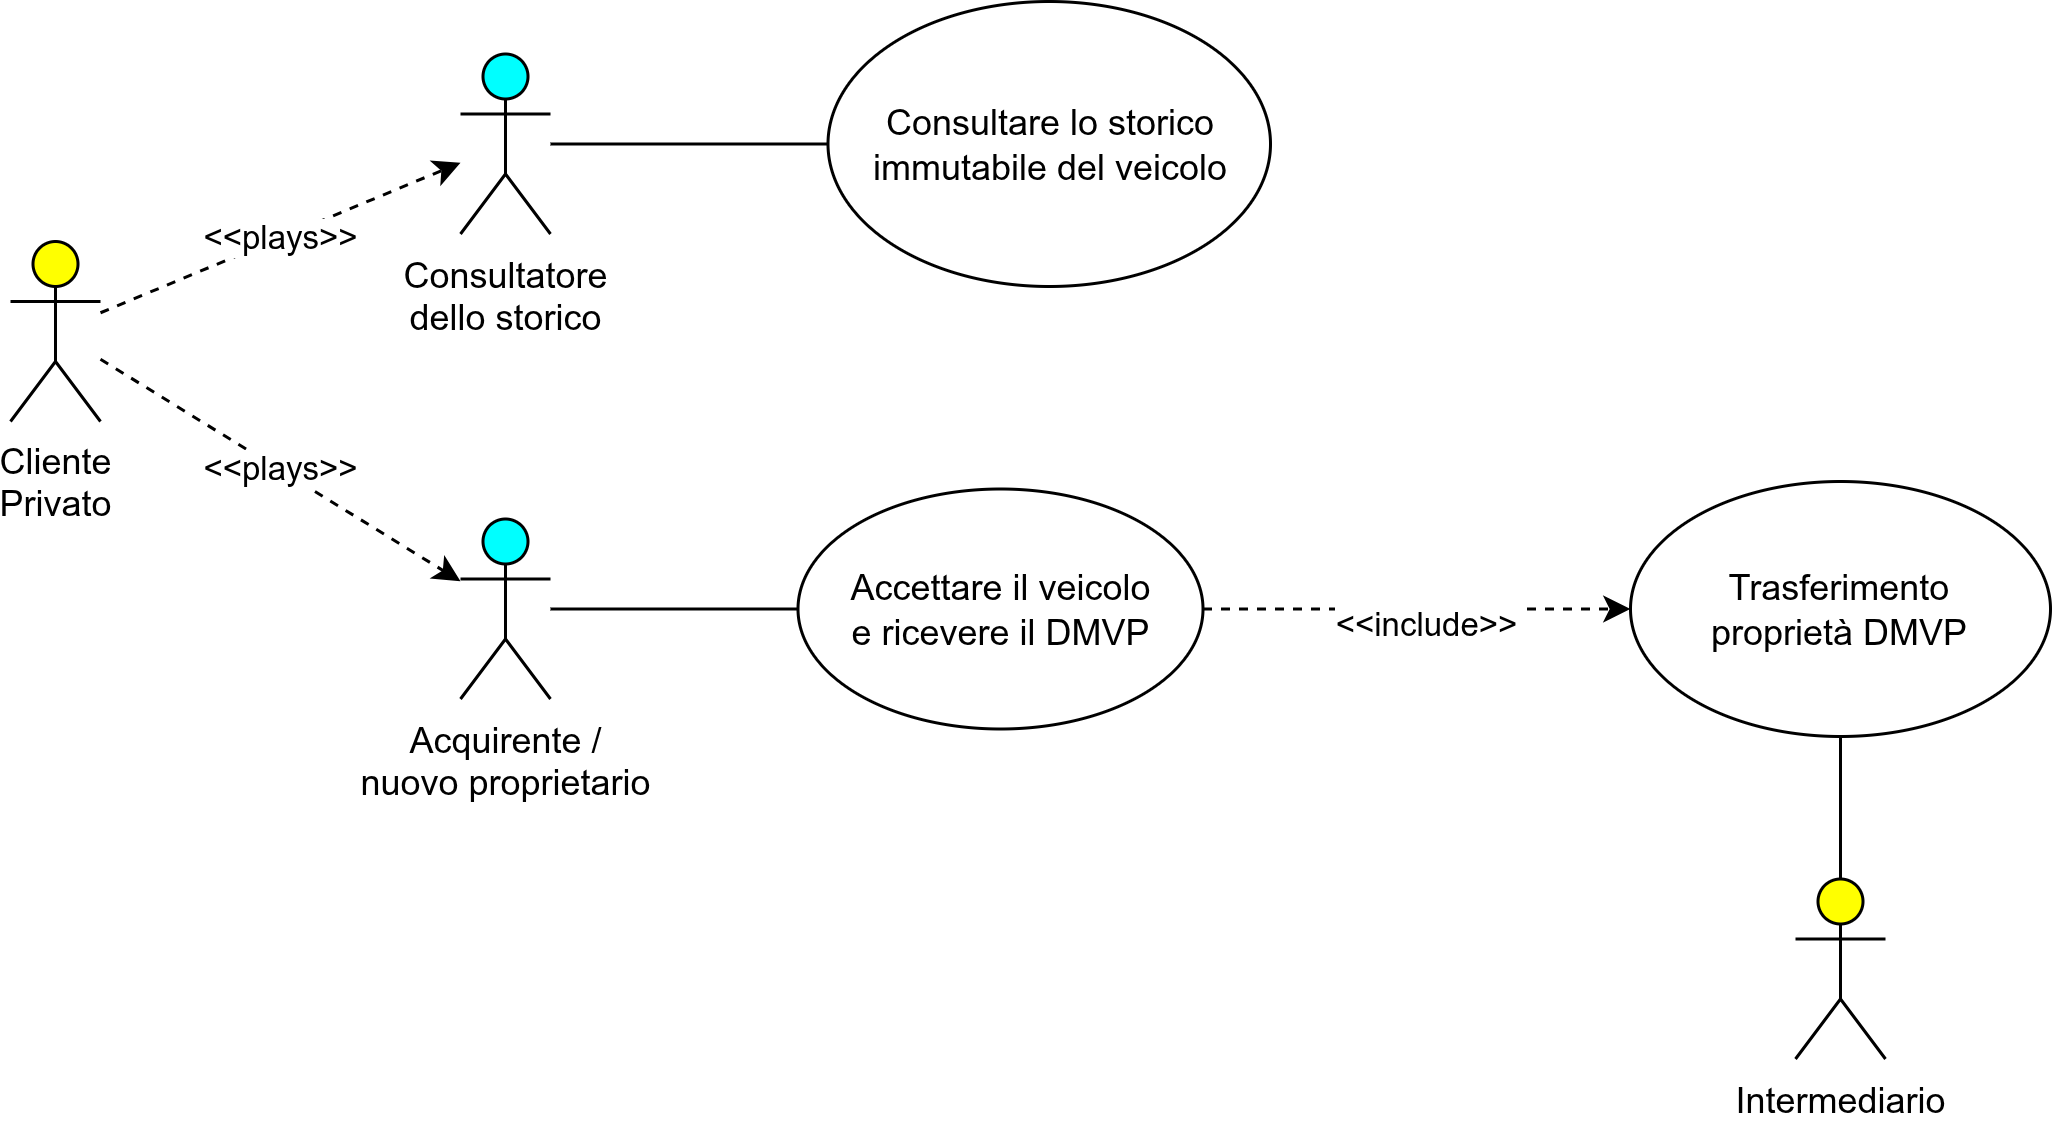
\includegraphics[width=\textwidth]{imgs/usecase/04_cliente_privato.png}
    \caption{Use-Case Cliente Privato}
    \label{fig:uc-cliente}
\end{figure}

\subsection*{Intermediario}

L'Intermediario, in qualità di gestore della piattaforma, gioca tre ruoli (Figura~\ref{fig:uc-intermediario}):

\begin{enumerate}
    \item \textit{Amministratore della piattaforma}, che configura e mantiene l'infrastruttura blockchain permissioned, definendo i canali, le politiche di \textit{endorsement} e i parametri di funzionamento della rete.
    \item \textit{Gestore delle identità e onboarding}, che registra e verifica le identità degli attori ammessi alla rete, emettendo le credenziali necessarie all'operatività sulla piattaforma. Si tratta del presupposto di affidabilità dell'intero sistema: soltanto soggetti verificati possono scrivere sul registro.
    \item \textit{Assistente all'uso della piattaforma}, che fornisce supporto operativo e formativo a tutti gli altri stakeholder. Tale use-case è infatti invocato da Concessionaria, Azienda di Tuning, Centro di Certificazione e Cliente Privato.
\end{enumerate}

\begin{figure}[H]
    \centering
    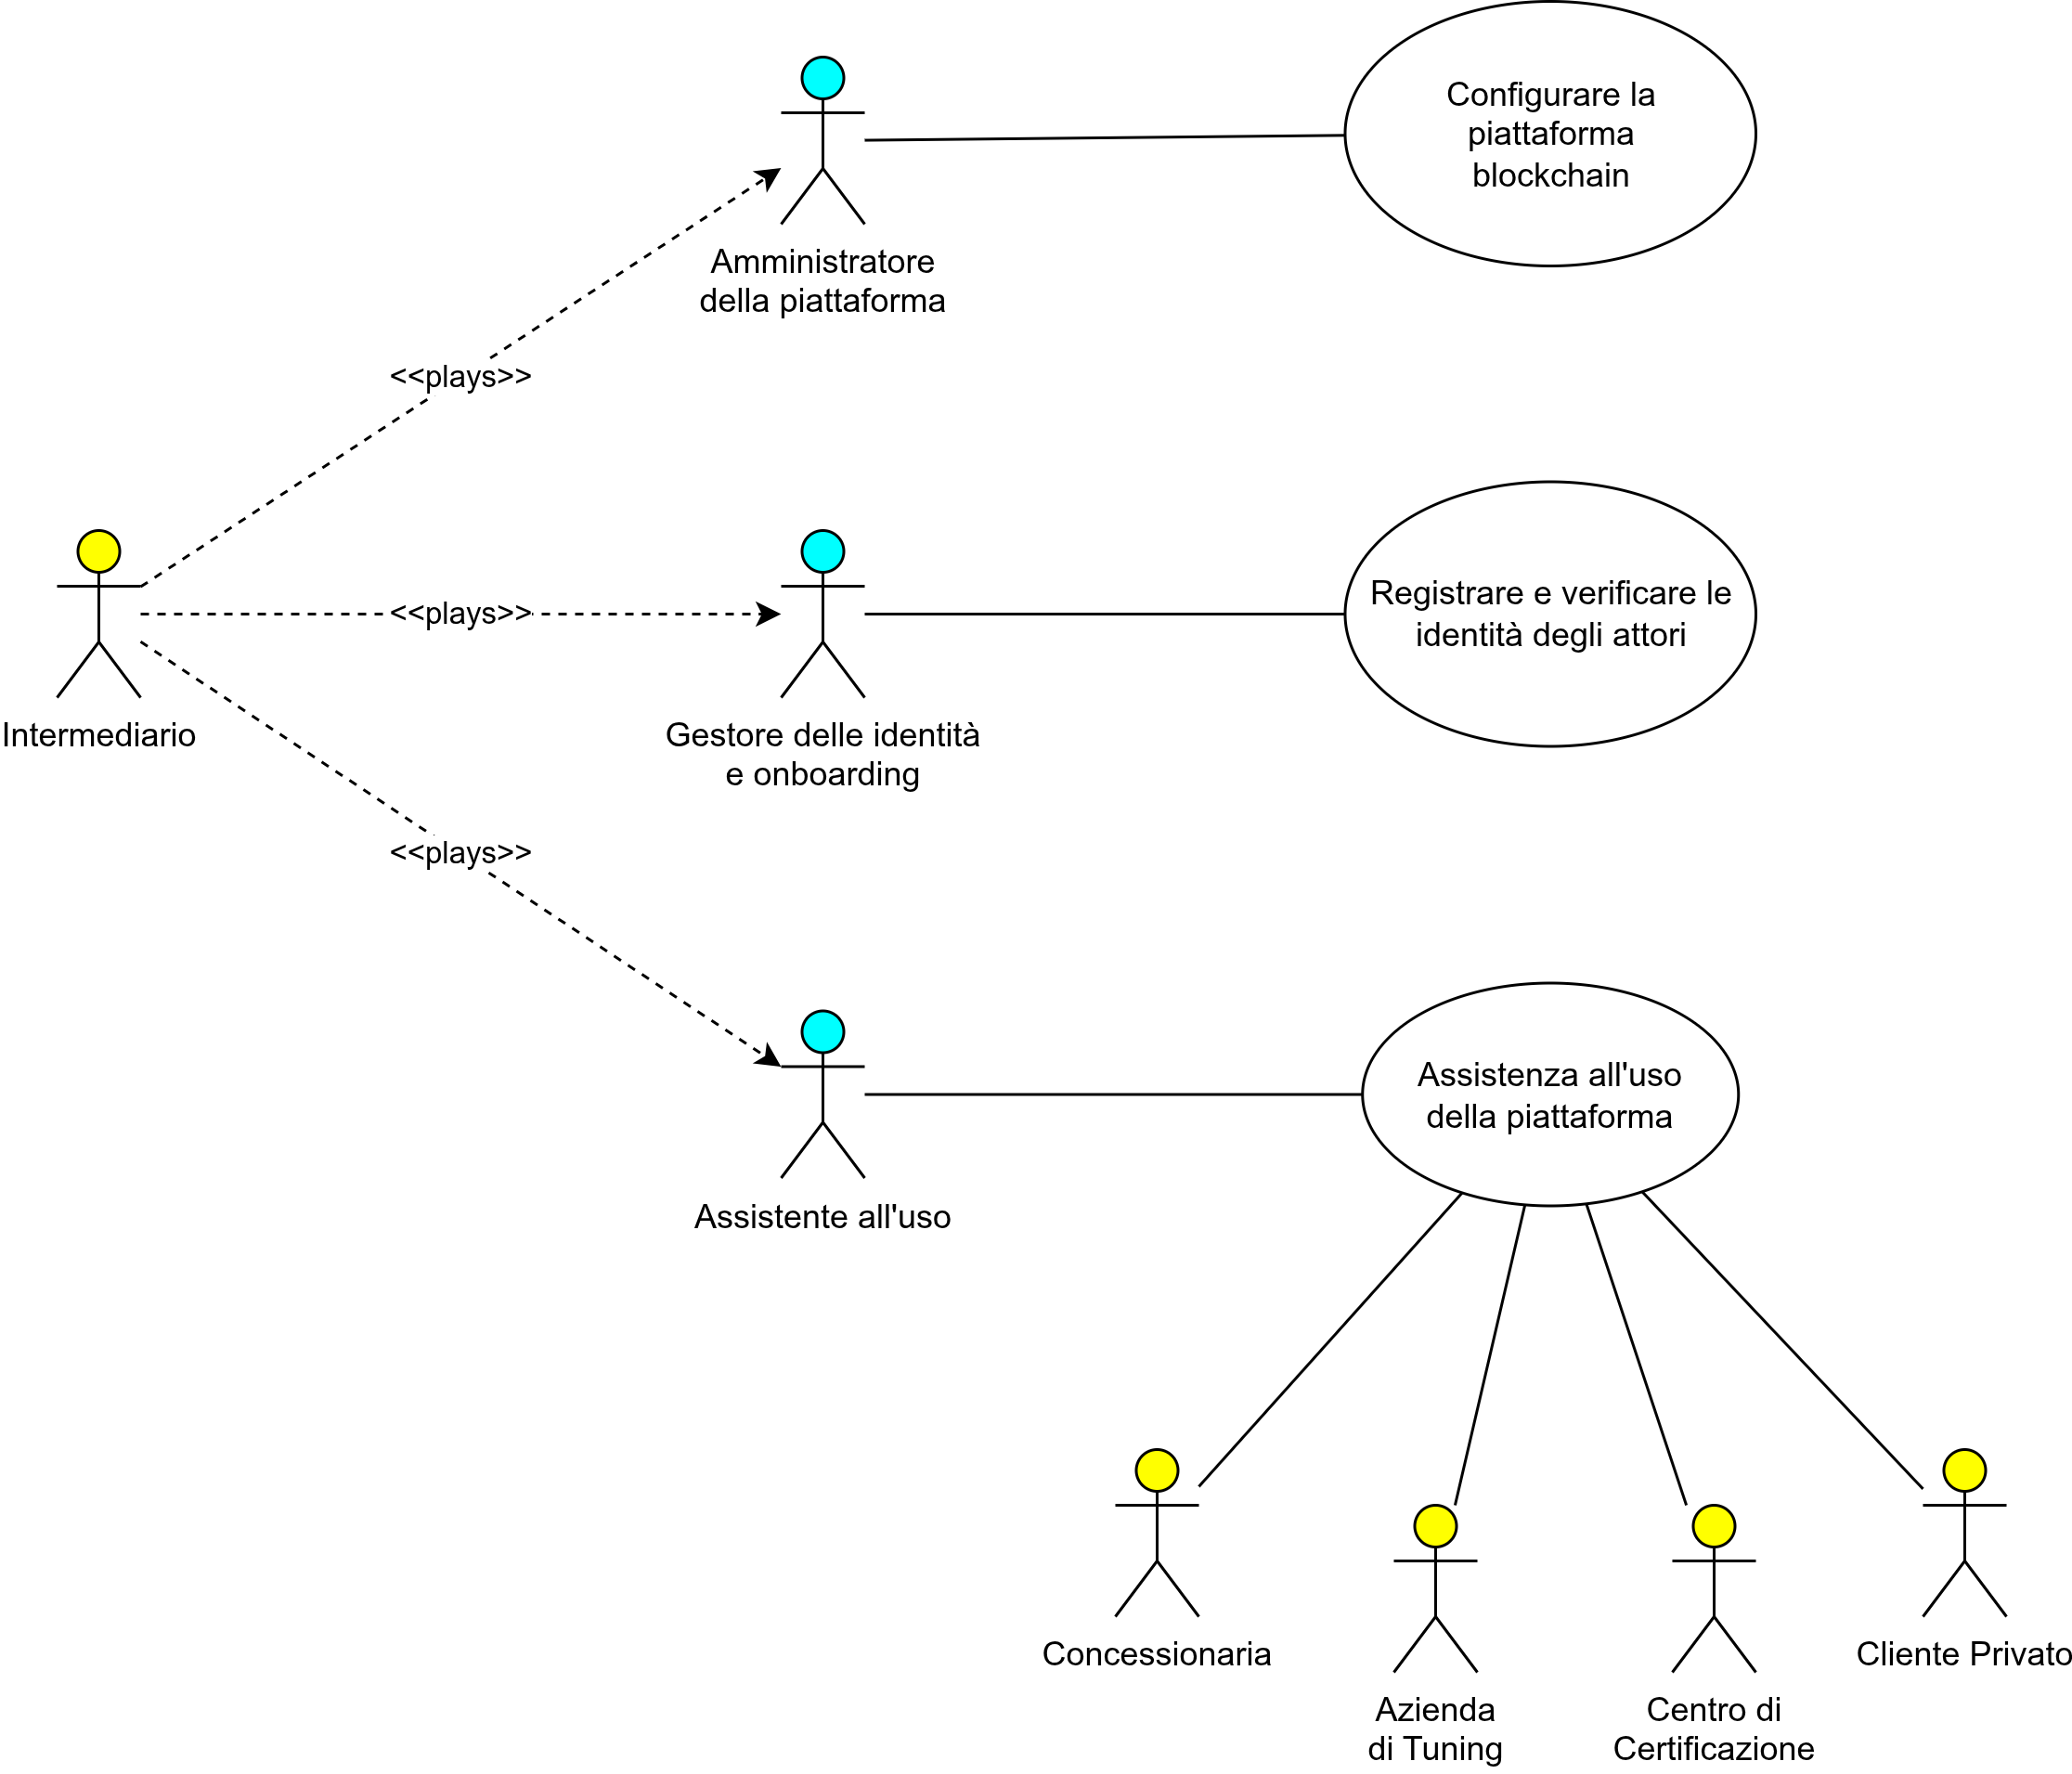
\includegraphics[width=\textwidth]{imgs/usecase/05_intermediario.png}
    \caption{Use-Case Intermediario}
    \label{fig:uc-intermediario}
\end{figure}

\section{Modellazione dei Processi principali in BPMN}

A valle della rappresentazione dei casi d'uso, è importante illustrare quali siano i processi fondamentali che avvengono all'interno della filiera in esame. A tal fine viene sfruttato il formalismo \textbf{BPMN} (\textit{Business Process Model and Notation}), rappresentazione grafica utilizzata per modellare e descrivere i processi aziendali. I diagrammi illustrano una coreografia, in cui ogni attività è svolta da un partecipante e indirizzata a uno o più altri partecipanti.

La modellazione dei processi ha l'obiettivo di:

\begin{itemize}
    \item rendere esplicite le responsabilità dei diversi attori coinvolti;
    \item descrivere il flusso informativo e decisionale lungo il ciclo di vita del veicolo modificato;
    \item evidenziare le interazioni tra la componente off-chain e l'infrastruttura blockchain;
    \item garantire la coerenza tra requisiti funzionali, casi d'uso e scelte tecnologiche.
\end{itemize}

In tutti i diagrammi la piattaforma, rappresentata dall'\textbf{Intermediario} e dall'infrastruttura blockchain sottostante, opera come componente di supporto trasversale, garantendo immutabilità dei dati, validazione delle informazioni e tracciabilità temporale delle operazioni. I due archivi di dati sono rappresentati distintamente: l'\textit{Off-Chain Database}, che conserva i dati descrittivi e i documenti, e la \textit{Blockchain}, sulla quale viene ancorata la sola impronta crittografica.

\subsection*{Processo Complessivo di Gestione del DMVP}

La Figura~\ref{fig:bpmn-complessivo} illustra l'architettura macroscopica del processo collaborativo, che descrive l'intero ciclo di vita del passaporto digitale dalla registrazione iniziale del veicolo fino al trasferimento finale della proprietà al cliente.

\begin{figure}[H]
    \centering
    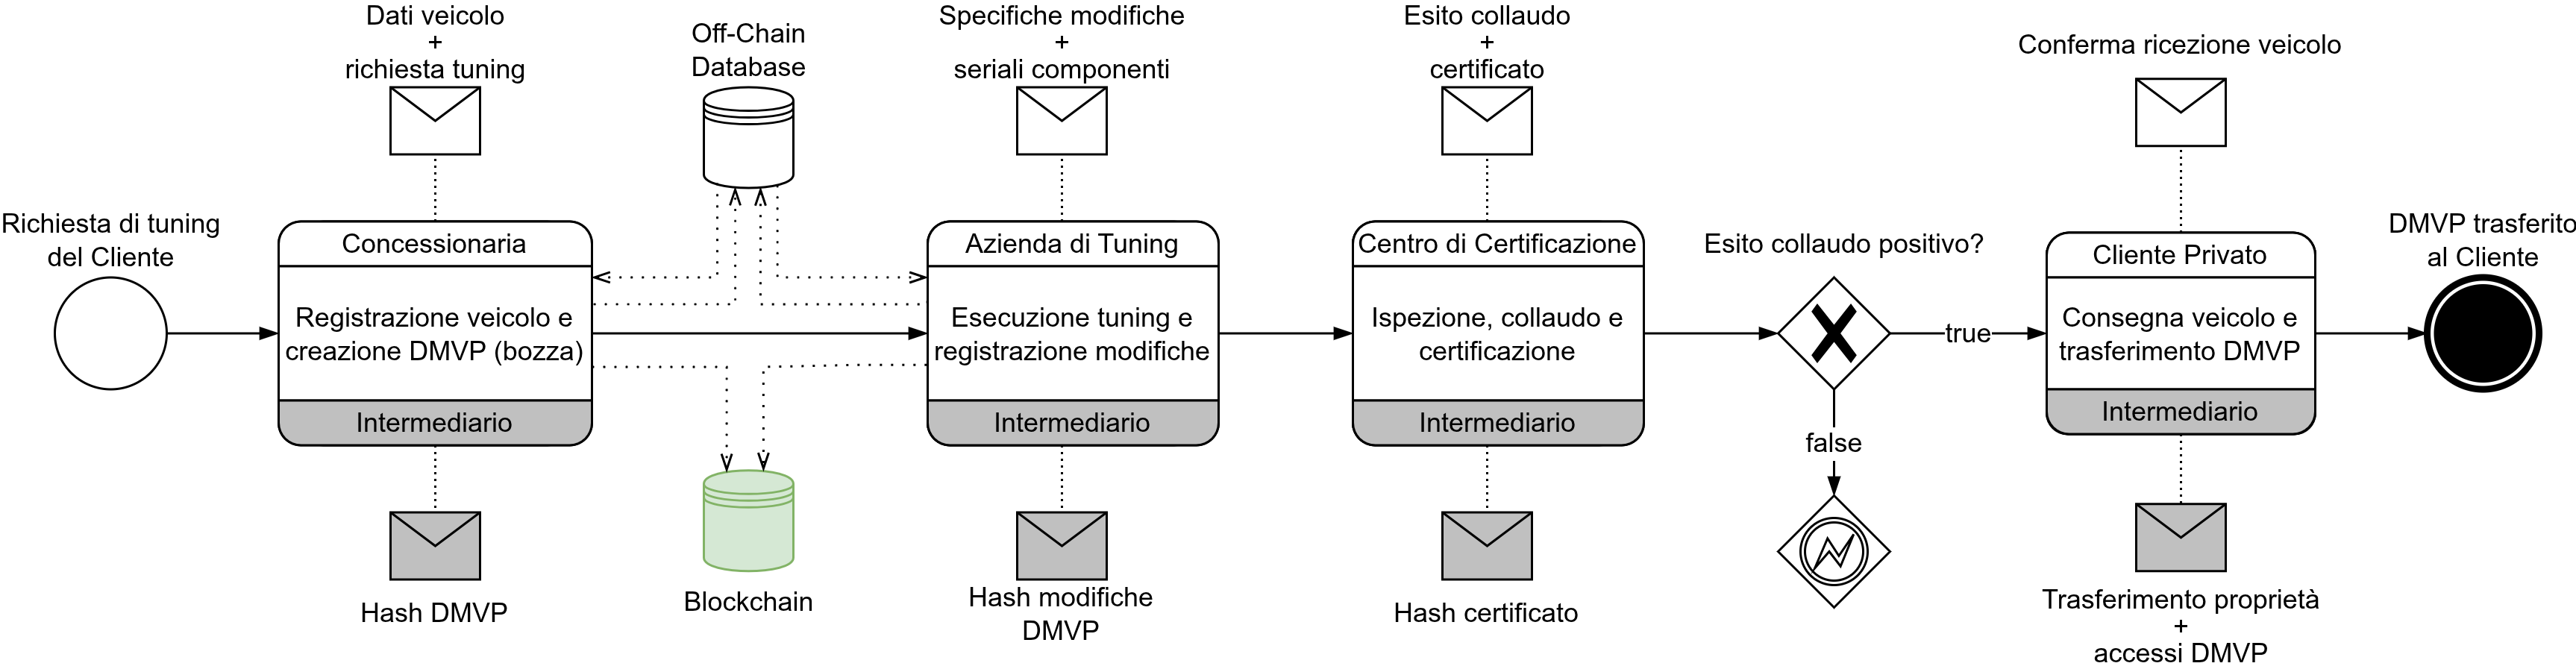
\includegraphics[width=\textwidth]{imgs/bpmn/00_gestione_DMVP.png}
    \caption{Processo complessivo di gestione del DMVP}
    \label{fig:bpmn-complessivo}
\end{figure}

Il flusso ha un andamento sequenziale e può essere idealmente suddiviso in quattro macro-fasi:

\begin{enumerate}
    \item \textbf{Registrazione del veicolo e creazione del DMVP}: l'innesco del processo avviene con la richiesta di tuning formulata dal Cliente Privato. La Concessionaria registra il veicolo base e genera una prima istanza del DMVP in stato di bozza, il cui hash viene ancorato sulla catena.
    \item \textbf{Esecuzione del tuning e registrazione delle modifiche}: l'Azienda di Tuning esegue le lavorazioni e ne registra le specifiche tecniche insieme ai seriali dei componenti installati, ancorando l'hash delle modifiche al DMVP.
    \item \textbf{Ispezione, collaudo e certificazione}: il Centro di Certificazione verifica la conformità tecnica e normativa degli interventi. Un \textit{Gateway Esclusivo} discrimina l'esito del collaudo: in caso negativo il processo termina con un evento di eccezione che rimanda le lavorazioni all'Azienda di Tuning; in caso positivo viene emesso il certificato digitale e il relativo hash viene registrato sulla catena.
    \item \textbf{Consegna e trasferimento}: il processo si conclude con la consegna del veicolo omologato e il trasferimento definitivo della proprietà e dei diritti di accesso al DMVP all'account del Cliente Privato.
\end{enumerate}

Al fine di garantire l'autenticità e l'affidabilità delle informazioni, ogni trasferimento di responsabilità o cambio di stato rilevante tra i soggetti della filiera viene ancorato in maniera indelebile sulla blockchain. Di seguito vengono analizzati i quattro sotto-processi di dettaglio.

\subsection*{Processo di Registrazione del Veicolo e Richiesta di Tuning}

Questo processo modella la fase di inizializzazione del passaporto digitale. Il flusso ha inizio nel momento in cui il Cliente Privato formalizza l'acquisto del veicolo e richiede una personalizzazione presso la Concessionaria, che avvia la procedura sulla piattaforma.

All'interno del diagramma di Figura~\ref{fig:bpmn-registrazione}, la Concessionaria inserisce i dati identificativi del veicolo e le modifiche richieste; la piattaforma esegue quindi una verifica di completezza dei dati, modellata come sotto-processo. Un \textbf{Gateway Esclusivo (XOR)} discrimina tra dati validi e dati incompleti: in caso di esito negativo il flusso viene reindirizzato, tramite un gateway di merge, all'attività di inserimento, richiedendo una nuova compilazione.

In caso di esito positivo, il processo prevede l'attivazione dell'Intermediario, che salva i dati descrittivi nel database off-chain e genera una prima transazione su blockchain per ancorare temporalmente la richiesta. Il processo si conclude con la notifica di presa in carico inviata all'Azienda di Tuning.

\begin{figure}[H]
    \centering
    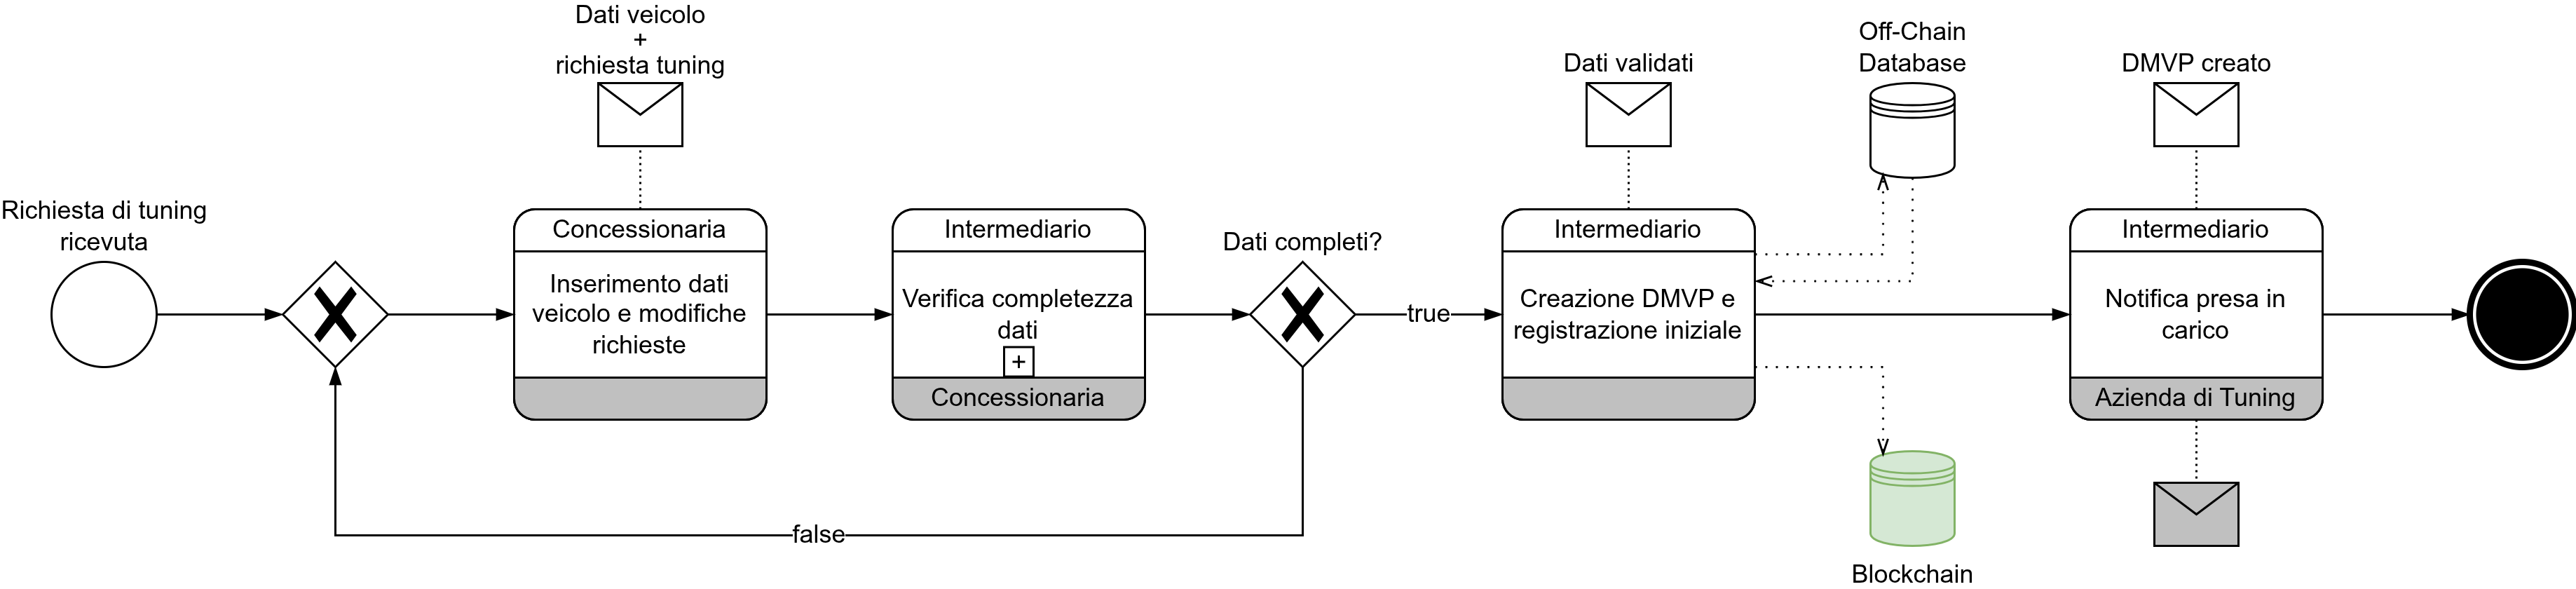
\includegraphics[width=\textwidth]{imgs/bpmn/01_registrazione_veicolo_e_richiesta_tuning.png}
    \caption{Processo di registrazione del veicolo e richiesta di tuning}
    \label{fig:bpmn-registrazione}
\end{figure}

\subsection*{Processo di Esecuzione del Tuning e Registrazione delle Modifiche}

Il diagramma di Figura~\ref{fig:bpmn-tuning} rappresenta il cuore operativo della piattaforma, descrivendo la fase di personalizzazione del veicolo. Il processo è attivato dalla ricezione della richiesta di lavorazione da parte dell'Azienda di Tuning.

Il flusso si articola in due macro-attività eseguite in parallelo, modellate tramite un \textbf{Gateway Parallelo (AND)}: l'esecuzione fisica delle modifiche sul veicolo, rappresentata come sotto-processo, e la rendicontazione digitale delle lavorazioni effettuate. In quest'ultima l'Azienda di Tuning inserisce le specifiche tecniche degli interventi, i codici seriali dei componenti installati e la documentazione tecnica associata.

La piattaforma provvede quindi al salvataggio strutturato delle informazioni nel database off-chain e alla registrazione del relativo hash sulla blockchain, garantendo l'immutabilità e la tracciabilità delle modifiche. I due rami convergono in un gateway di sincronizzazione e il processo si conclude con l'invio automatico di una notifica al Centro di Certificazione, che avvia la fase di collaudo.

\begin{figure}[H]
    \centering
    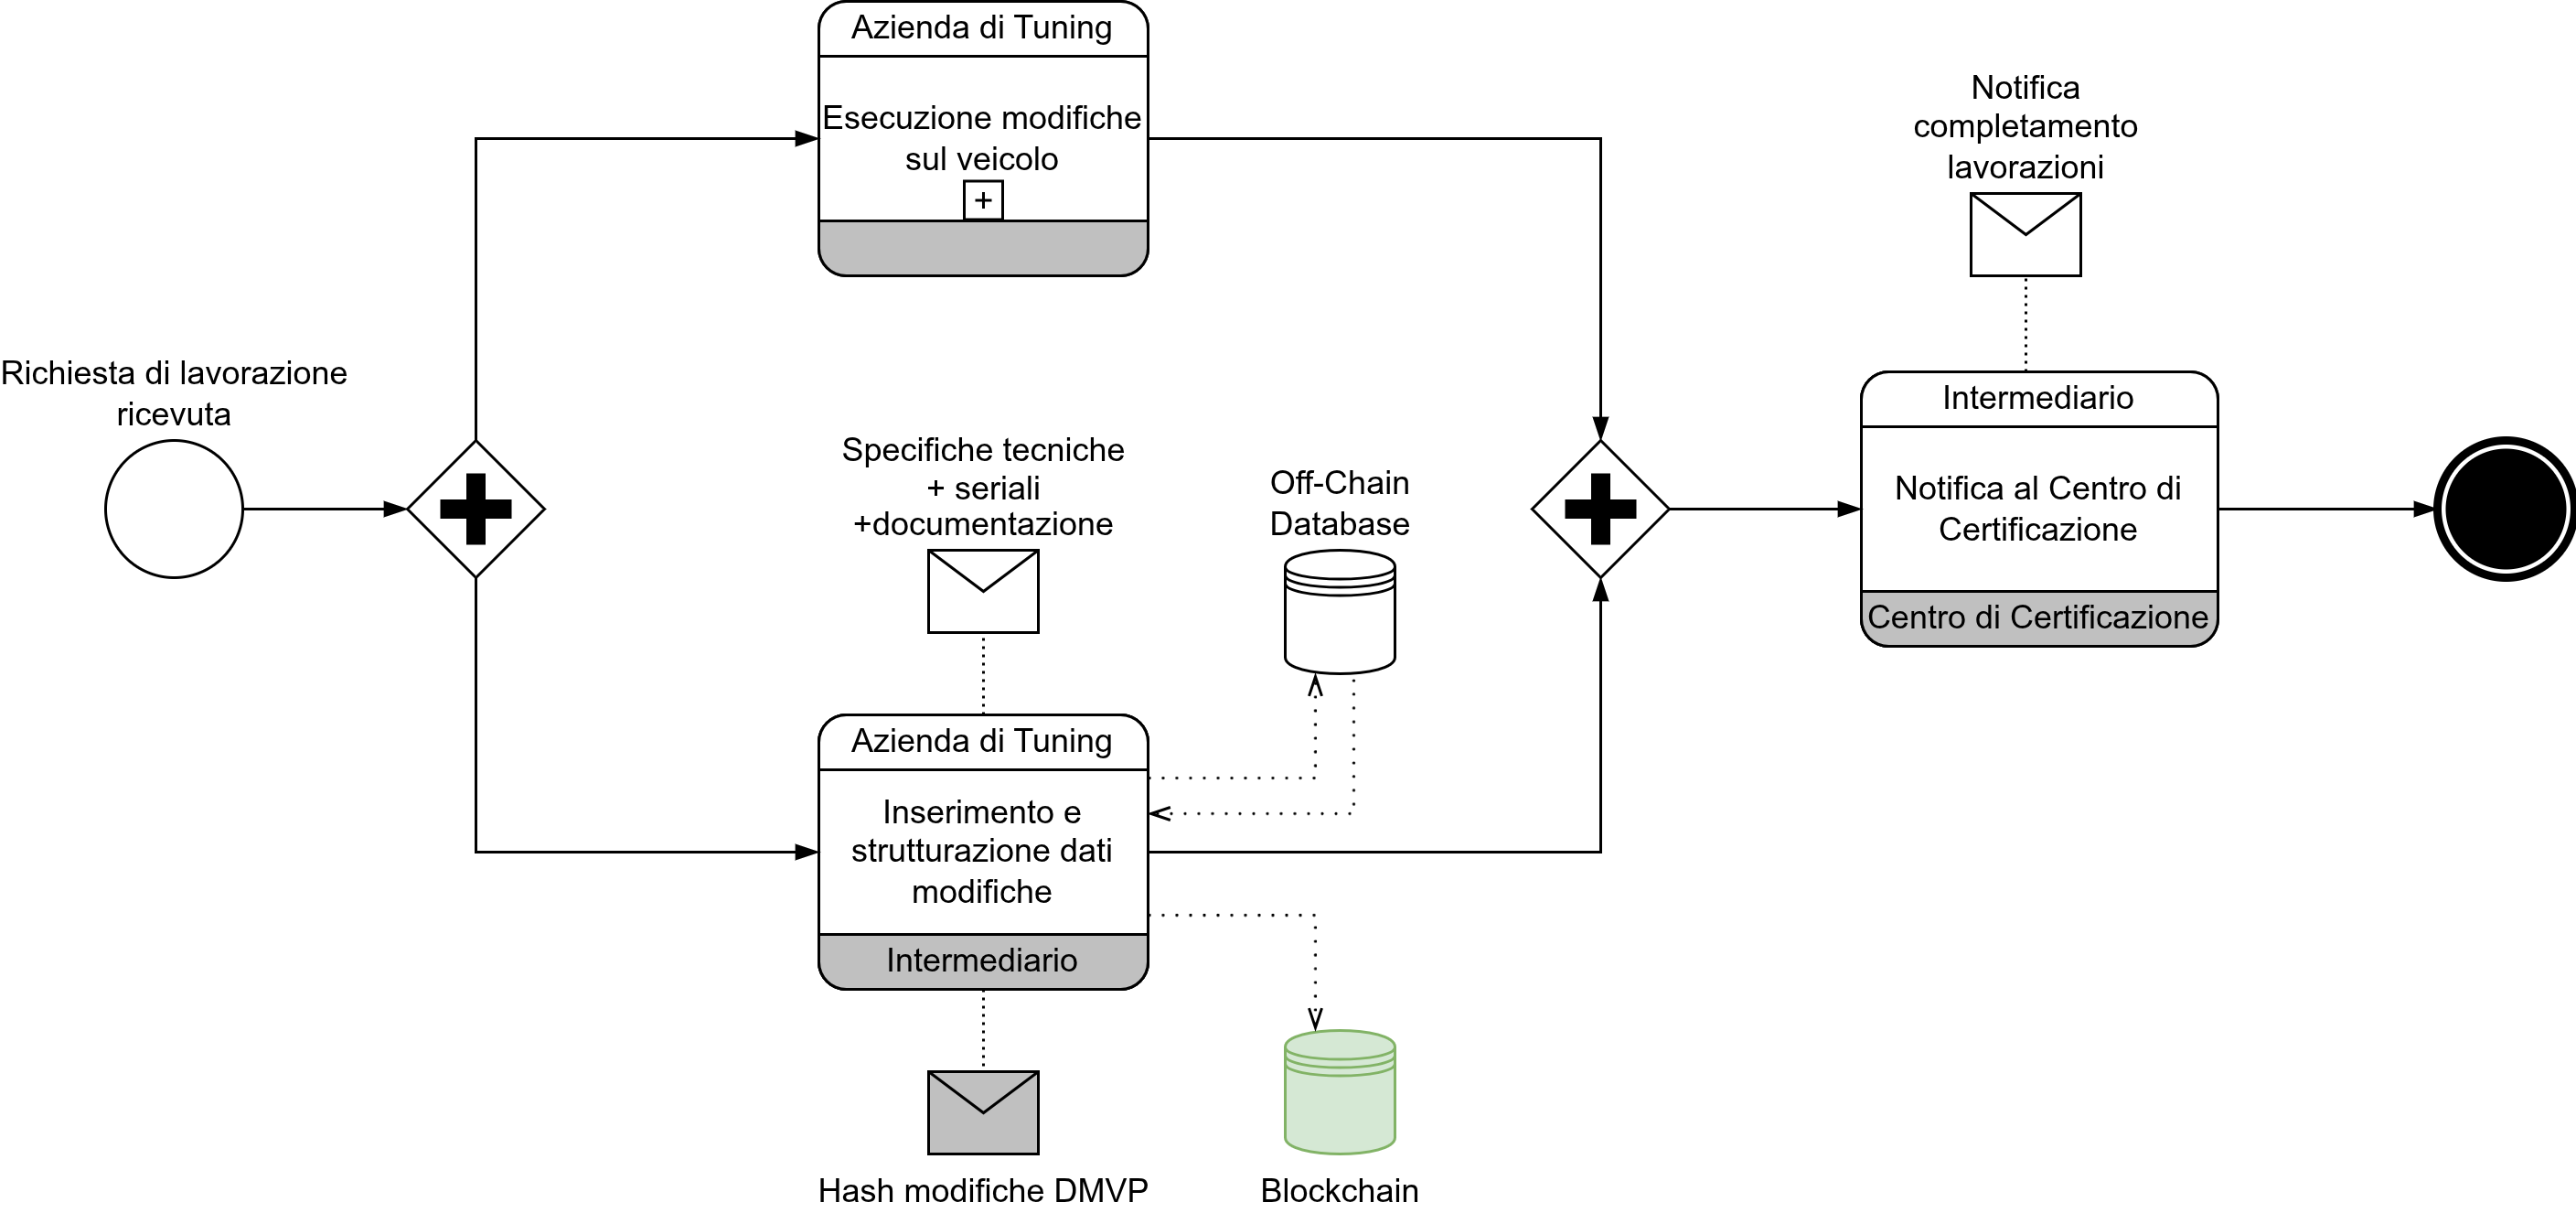
\includegraphics[width=\textwidth]{imgs/bpmn/02_esecuzione_tuning_e_registrazione_modifiche.png}
    \caption{Processo di esecuzione del tuning e registrazione delle modifiche}
    \label{fig:bpmn-tuning}
\end{figure}

\subsection*{Processo di Ispezione e Certificazione}

Il terzo processo (Figura~\ref{fig:bpmn-certificazione}) formalizza la fase di ispezione tecnica e certificazione normativa. Il flusso ha inizio con la presa in carico del veicolo da parte del Centro di Certificazione, che consulta i dati storici del DMVP registrati sulla piattaforma ed esegue le verifiche tecniche e normative previste, modellate come sotto-processo.

Un \textbf{Gateway Esclusivo (XOR)} gestisce l'esito dell'ispezione:

\begin{itemize}
    \item \textbf{Caso negativo}: le modifiche risultano non conformi. Viene generato un report di anomalia e il ramo termina con un \textit{Message End Event} indirizzato all'Azienda di Tuning, alla quale la pratica viene reindirizzata per le necessarie correzioni.
    \item \textbf{Caso positivo}: il collaudo è superato e viene emesso il certificato digitale.
\end{itemize}

In caso di esito positivo il certificato viene archiviato nel database off-chain, mentre il relativo hash crittografico viene registrato sulla blockchain tramite l'Intermediario. Il processo si conclude con l'aggiornamento dello stato del DMVP a \textit{Certificato e Conforme}.

\begin{figure}[H]
    \centering
    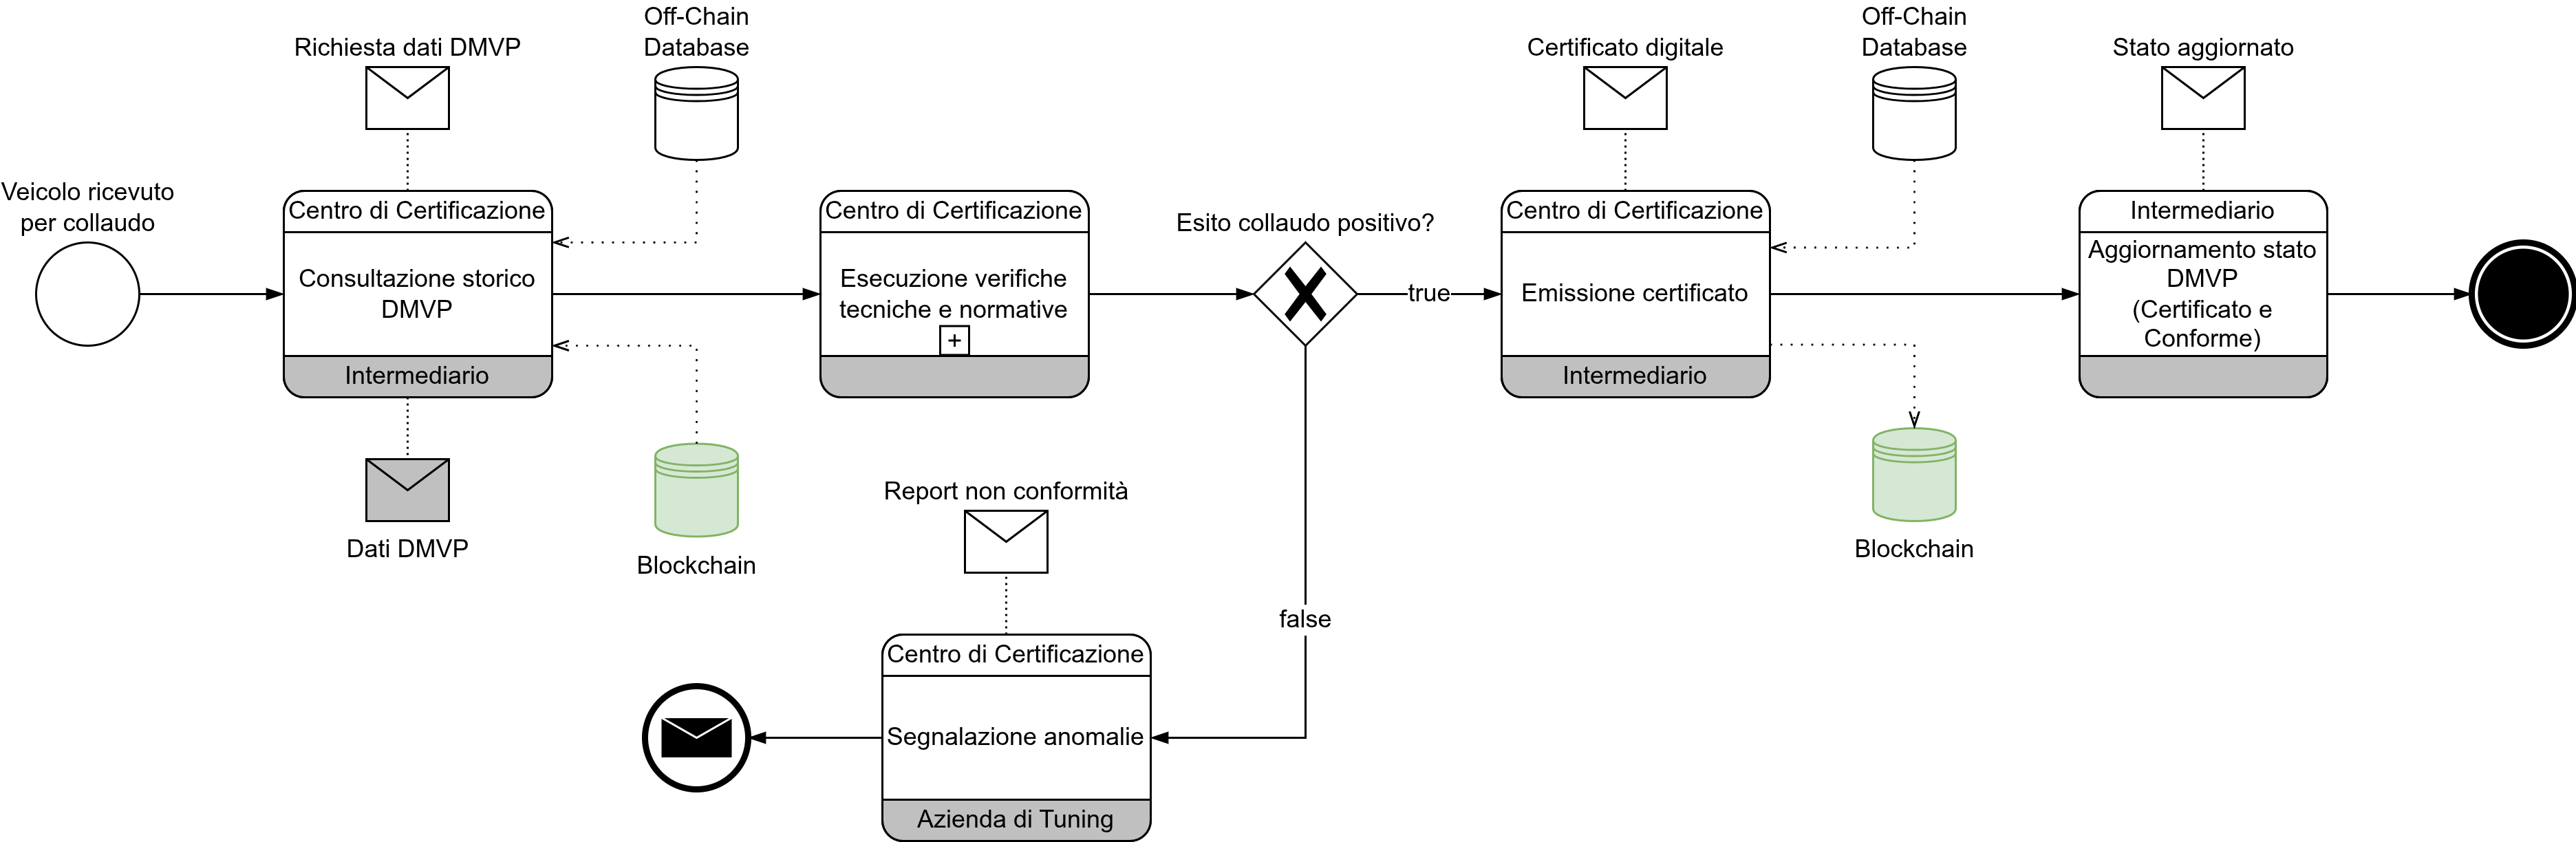
\includegraphics[width=\textwidth]{imgs/bpmn/03_ispezione_e_certificazione.png}
    \caption{Processo di ispezione e certificazione}
    \label{fig:bpmn-certificazione}
\end{figure}

\subsection*{Processo di Consegna del Veicolo e Trasferimento del DMVP}

L'ultimo processo (Figura~\ref{fig:bpmn-consegna}) modella la fase di consegna finale del veicolo e il trasferimento del passaporto digitale al Cliente Privato. Il flusso è avviato dalla Concessionaria a seguito della ricezione del veicolo omologato.

Il processo prevede la predisposizione del veicolo per la consegna finale, la consultazione dello storico del DMVP da parte del Cliente Privato --- che accede ai dati descrittivi conservati off-chain e ne verifica l'integrità sulla catena --- e infine l'accettazione formale del veicolo.

L'accettazione del cliente attiva l'operazione gestita dall'Intermediario attraverso la quale vengono trasferiti sulla blockchain i diritti di accesso e la proprietà del DMVP. L'evento finale segna la chiusura dell'intero ciclo di tracciabilità post-vendita del veicolo modificato.

\begin{figure}[H]
    \centering
    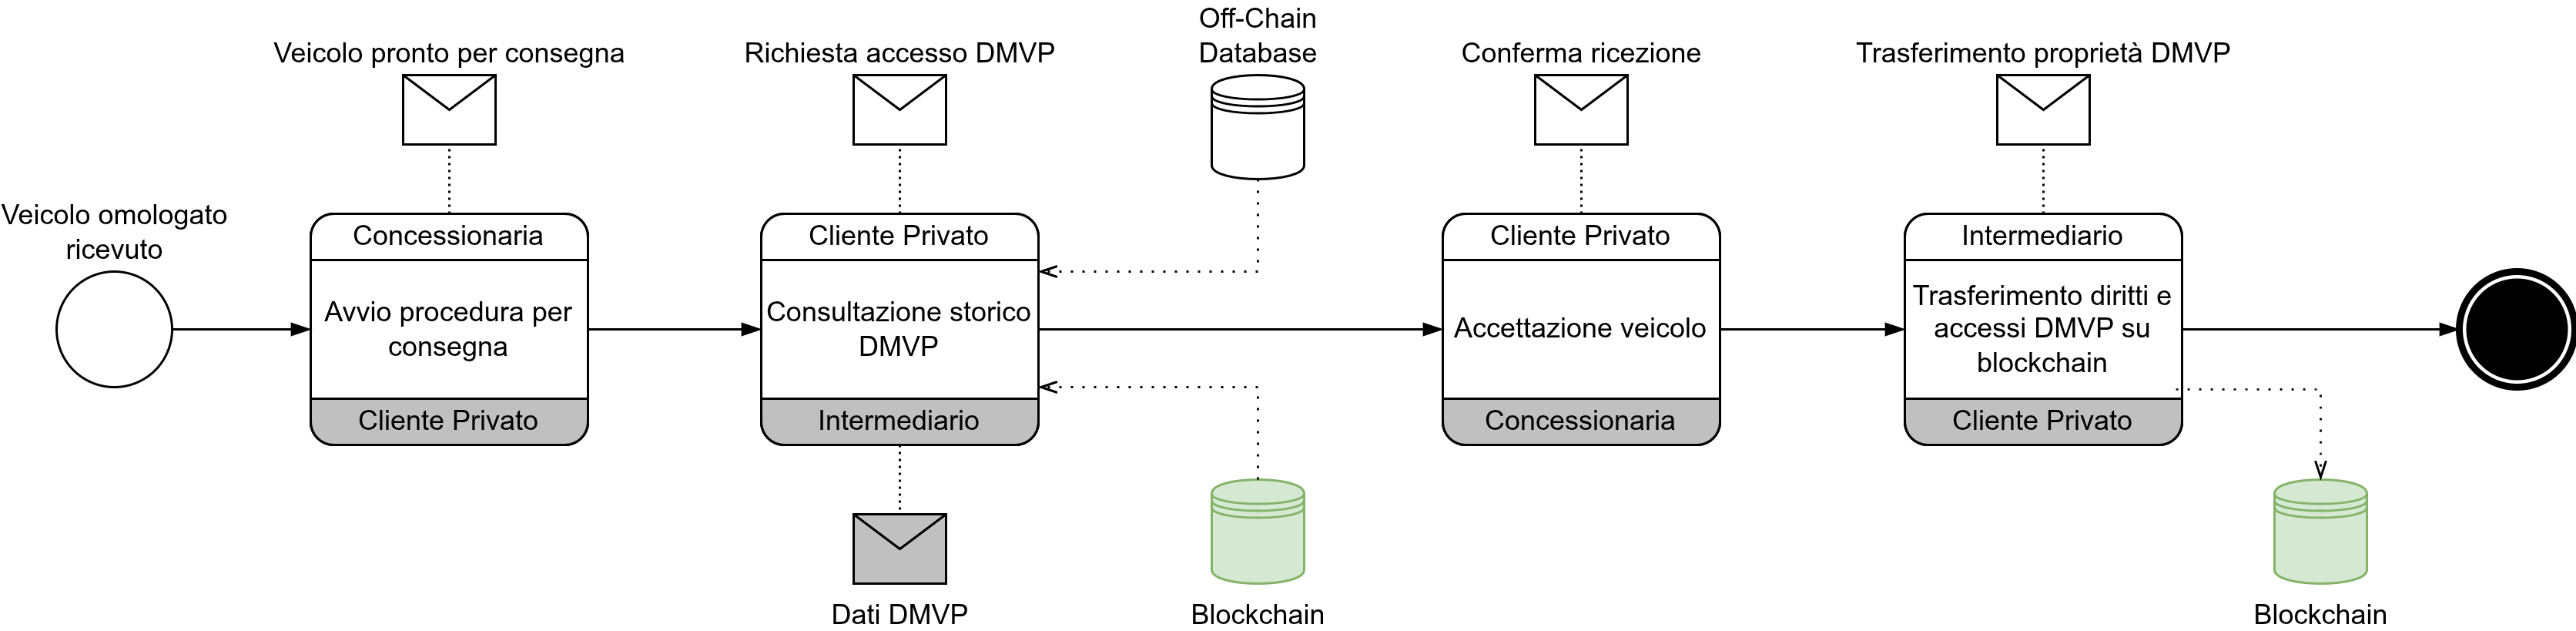
\includegraphics[width=\textwidth]{imgs/bpmn/04_consegna_veicolo_e_trasferimento_DMVP.png}
    \caption{Processo di consegna del veicolo e trasferimento del DMVP}
    \label{fig:bpmn-consegna}
\end{figure}
\chapter{Analisi SWOT}
\section{Analisi SWOT di opportunità, minacce, punti di forza e punti di debolezza}

La \textbf{Figura~\ref{fig:swot}} riassume l'analisi SWOT dell'idea progettuale in esame.

\begin{figure}[H]
    \centering
    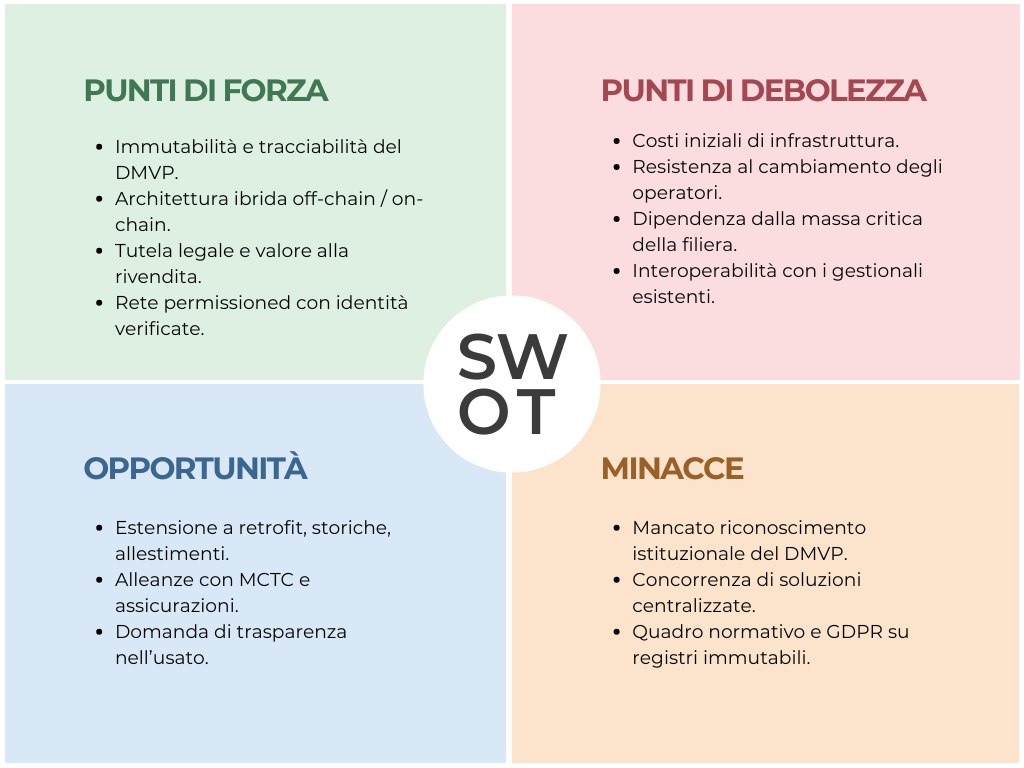
\includegraphics[width=\textwidth]{imgs/swot.png}
    \caption{Analisi SWOT}
    \label{fig:swot}
\end{figure}

L'analisi SWOT mette in luce i punti di forza, le debolezze, le opportunità e le minacce di \textit{Tuning Ledger}, la piattaforma per la gestione del \textit{Digital Modified Vehicle Passport} (DMVP) basata su blockchain permissioned. Di seguito vengono esaminati i principali aspetti che caratterizzano il progetto.

\subsection*{Punti di Forza}
Il sistema offre numerosi vantaggi che ne aumentano il valore e la competitività nel settore dell'automotive tuning. In particolare:

\begin{enumerate}
    \item \textbf{Immutabilità e tracciabilità del passaporto digitale}: grazie all'ancoraggio degli hash sul registro distribuito, ogni fase del ciclo di vita del veicolo modificato -- dalla registrazione del veicolo base alla certificazione delle modifiche -- risulta verificabile e non alterabile. Ciò azzera la possibilità di retrodatare interventi, sostituire documentazione tecnica o dichiarare modifiche mai eseguite.

    \item \textbf{Architettura ibrida off-chain/on-chain}: la separazione tra i dati descrittivi voluminosi (schede tecniche, documentazione fotografica, certificati), conservati nel database off-chain, e le relative impronte crittografiche registrate on-chain consente di coniugare l'integrità garantita dalla blockchain con l'efficienza e la sostenibilità economica dell'archiviazione tradizionale, senza gravare sulle prestazioni della rete.

    \item \textbf{Tutela legale degli attori e valorizzazione del veicolo}: la registrazione immutabile delle lavorazioni costituisce una prova documentale a favore dell'Azienda di Tuning contro contestazioni infondate, riduce il rischio legale della Concessionaria in caso di modifiche non conformi e fornisce al Cliente Privato uno storico certificato che accresce il valore del veicolo al momento della rivendita.

    \item \textbf{Rete permissioned con identità verificate}: l'adozione di una blockchain ad accesso controllato, in cui l'Intermediario verifica preventivamente l'identità di tutti gli attori B2B ammessi, garantisce l'affidabilità della fonte di ogni registrazione e agevola il coinvolgimento di intermediari esperti, capaci di trasferire innovazione digitale verso gli operatori del settore.
\end{enumerate}

\subsection*{Punti di Debolezza}
Nonostante i vantaggi, l'implementazione del sistema presenta alcune criticità che potrebbero limitarne la diffusione e l'adozione da parte degli attori della filiera. In particolare:

\begin{enumerate}
    \item \textbf{Costi di implementazione e infrastruttura}: lo sviluppo della piattaforma, l'esercizio dei nodi della rete permissioned e l'integrazione con i sistemi esistenti richiedono investimenti iniziali elevati, che rappresentano una barriera economica significativa per le officine di tuning di piccole dimensioni e per le realtà artigianali.

    \item \textbf{Resistenza al cambiamento degli operatori}: l'introduzione di procedure digitali strutturate, che impongono la rendicontazione puntuale di ogni lavorazione e componente installato, potrebbe incontrare resistenze da parte di operatori abituati a una gestione informale o cartacea della documentazione tecnica.

    \item \textbf{Dipendenza dalla massa critica della filiera}: il valore della piattaforma cresce con il numero di attori aderenti. Se i Centri di Certificazione o le Concessionarie non partecipassero attivamente, il DMVP resterebbe incompleto e perderebbe la propria funzione di fonte unica e certificata della verità; a ciò si aggiunge una forte dipendenza operativa dall'Intermediario, unico soggetto responsabile della governance della rete.

    \item \textbf{Scalabilità e interoperabilità}: l'integrazione con i sistemi gestionali eterogenei già in uso presso concessionarie, officine ed enti di certificazione, spesso proprietari e non standardizzati, può presentare complessità tecniche in fase di configurazione dei canali di comunicazione.
\end{enumerate}

\subsection*{Opportunità}
L'evoluzione del mercato e l'attenzione crescente verso la trasparenza e la conformità normativa offrono numerose opportunità di crescita e sviluppo per il sistema. In particolare:

\begin{enumerate}
    \item \textbf{Espansione del mercato}: il modello del passaporto digitale può essere esteso oltre il tuning tradizionale verso ambiti affini e in forte crescita, quali il retrofit elettrico, il restauro e la certificazione dei veicoli storici, l'allestimento di veicoli commerciali e la gestione documentale delle flotte aziendali, ampliando in modo significativo il bacino d'utenza.

    \item \textbf{Disponibilità di collaborazioni strategiche}: la possibilità di creare alleanze con la Motorizzazione Civile, con le associazioni di categoria del settore, con le compagnie assicurative e con organizzazioni di promozione della tecnologia DLT aumenta la credibilità del sistema e potrebbe favorirne l'adozione come standard di riferimento per la documentazione delle modifiche.

    \item \textbf{Crescente domanda di trasparenza e conformità}: acquirenti, compagnie assicurative e autorità di controllo richiedono garanzie sempre maggiori sulla storia e sulla regolarità dei veicoli, soprattutto nel mercato dell'usato. Questa tendenza, rafforzata dalla progressiva diffusione dei passaporti digitali di prodotto~\cite{espr}, rappresenta un'opportunità rilevante per il sistema, che risponde in modo nativo a tali requisiti attraverso la certificazione digitale del ciclo di vita del veicolo modificato.
\end{enumerate}

\subsection*{Minacce}
Infine, ci sono alcune minacce esterne che potrebbero ostacolare la diffusione del sistema o limitarne il potenziale complessivo. In particolare:

\begin{enumerate}
    \item \textbf{Mancato riconoscimento istituzionale del DMVP}: in assenza di un valore formale attribuito al passaporto digitale da parte della Motorizzazione Civile e delle compagnie assicurative, il DMVP rischia di configurarsi come un adempimento aggiuntivo rispetto alla documentazione cartacea già obbligatoria, anziché sostitutivo di essa. Ne deriverebbe, per gli operatori della filiera, un costo privo di un ritorno immediato e percepibile, con un conseguente rallentamento dell'adozione volontaria della piattaforma.

    \item \textbf{Concorrenza di soluzioni alternative}: operatori software già consolidati nella gestione delle officine e delle concessionarie potrebbero integrare funzionalità di tracciamento proprietarie e centralizzate, meno costose da adottare; parallelamente, le case automobilistiche potrebbero sviluppare passaporti digitali interni al proprio ecosistema, riducendo temporaneamente il vantaggio competitivo della soluzione decentralizzata.

    \item \textbf{Evoluzione normativa e ostacoli legali}: la disciplina sul valore probatorio delle registrazioni su blockchain è in continua evoluzione a livello nazionale ed europeo, così come i requisiti di omologazione delle modifiche~\cite{cds,dpr495}, che variano tra i diversi ordinamenti. A ciò si aggiunge la tensione tra l'immutabilità del registro e gli obblighi in materia di protezione dei dati personali (in particolare il diritto alla cancellazione previsto dal GDPR), che potrebbe imporre modifiche architetturali complesse e rallentare la diffusione della piattaforma.
\end{enumerate}

\section{Valutazione finale dell'Idea Progettuale}

L'analisi SWOT ha evidenziato numerosi aspetti positivi dell'idea progettuale, supportando la decisione di procedere con lo sviluppo della piattaforma per la gestione del passaporto digitale del veicolo modificato basata su blockchain.

L'immutabilità del DMVP, l'efficienza dell'architettura ibrida off-chain/on-chain e la tutela legale offerta a tutti gli attori coinvolti rappresentano i principali punti di forza del progetto, confermando come esso risponda a una domanda di mercato in crescita e offra valore aggiunto lungo l'intera filiera, con un forte focus sulla conformità normativa e sulla certezza delle informazioni.

Tuttavia, l'analisi delle debolezze e delle minacce ha messo in luce alcuni aspetti critici che dovranno essere superati per garantire il successo della piattaforma. I costi di implementazione iniziali e la resistenza al cambiamento degli operatori, unitamente alla necessità di raggiungere una massa critica di attori aderenti, rappresentano le principali sfide. Per mitigare tali ostacoli sarà necessario incentivare un'adozione progressiva, introducendo interfacce d'uso semplificate e modelli di accesso graduali che permettano una transizione tecnologica sostenibile anche per le realtà di piccole dimensioni.

Inoltre, le opportunità di mercato rappresentano un elemento chiave per il successo del progetto. L'estensione del modello oltre il tuning tradizionale, verso il retrofit elettrico, i veicoli storici e l'allestimento di veicoli commerciali, permetterà di ampliare la base utenti e di aumentare la competitività della piattaforma. Allo stesso modo, collaborazioni strategiche con la Motorizzazione Civile, le associazioni di categoria e le compagnie assicurative potrebbero rafforzare la credibilità del sistema e incentivarne l'adozione su larga scala. Tali collaborazioni costituiscono, in particolare, la principale leva di mitigazione della minaccia relativa al mancato riconoscimento istituzionale del DMVP: solo l'attribuzione di un valore formale al passaporto digitale da parte degli enti competenti e del comparto assicurativo può trasformarlo da adempimento aggiuntivo in strumento sostitutivo della documentazione tradizionale, rendendo il beneficio immediatamente percepibile dagli operatori della filiera.

Infine, un fattore critico da considerare sarà l'evoluzione del quadro normativo relativo all'impiego della blockchain, in particolare per quanto concerne il valore legale delle registrazioni e la conformità al trattamento dei dati personali: questo potrebbe influenzare l'implementazione del sistema in diversi contesti geografici e amministrativi. Per prevenire eventuali ostacoli legali sarà necessario adattarsi dinamicamente ai cambiamenti normativi e garantire la conformità della piattaforma agli standard di tracciabilità e di omologazione vigenti.

La valutazione complessiva del progetto è positiva, nonostante le sfide da affrontare. Le strategie di mitigazione delle debolezze e delle minacce, unite alle opportunità di mercato e ai punti di forza della piattaforma, suggeriscono che lo sviluppo dell'idea progettuale sia vantaggioso.

I prossimi passi dovranno prevedere la realizzazione di un Project Plan dettagliato, con la definizione dell'architettura a componenti e delle fasi di implementazione, e di un Business Plan volto a valutare la sostenibilità economica dell'iniziativa e a massimizzare l'adozione della piattaforma nel settore dell'automotive tuning.
\chapter{Project Plan}

\section{Organizzazione Complessiva del Project Plan}

La realizzazione di \textit{Tuning Ledger}, la piattaforma per la gestione del \textit{Digital Modified Vehicle Passport} (DMVP), richiede una pianificazione dettagliata e suddivisa in fasi, al fine di garantire un avanzamento efficace del lavoro e un monitoraggio costante dei risultati.

Il Project Plan copre un arco temporale di sei anni ed è articolato in due fasi principali:

\begin{itemize}
    \item \textbf{Prima Fase: progettazione, sviluppo e deployment della piattaforma.}
    \begin{itemize}
        \item \textit{Descrizione}: realizzazione completa del sistema informativo, comprensiva dell'infrastruttura blockchain permissioned, dei micro-servizi applicativi e delle interfacce destinate agli attori della filiera.
        \item \textit{Durata}: 1 anno.
    \end{itemize}
    \item \textbf{Seconda Fase: promozione, esercizio e mantenimento della piattaforma.}
    \begin{itemize}
        \item \textit{Descrizione}: a seguito del rilascio, la piattaforma entra in una fase di espansione commerciale e operativa nel mercato dell'automotive tuning, durante la quale vengono erogate le attività di supporto tecnico, onboarding degli attori, analisi dei dati di esercizio e sviluppo continuo per l'adeguamento normativo.
        \item \textit{Durata}: 5 anni.
    \end{itemize}
\end{itemize}

Le due fasi hanno inizio il 1\textdegree{} gennaio 2026 e termine il 31 dicembre 2031, come riassunto nel diagramma di GANTT complessivo riportato in Figura~\ref{fig:gantt-complessivo}.

\begin{figure}[H]
    \centering
    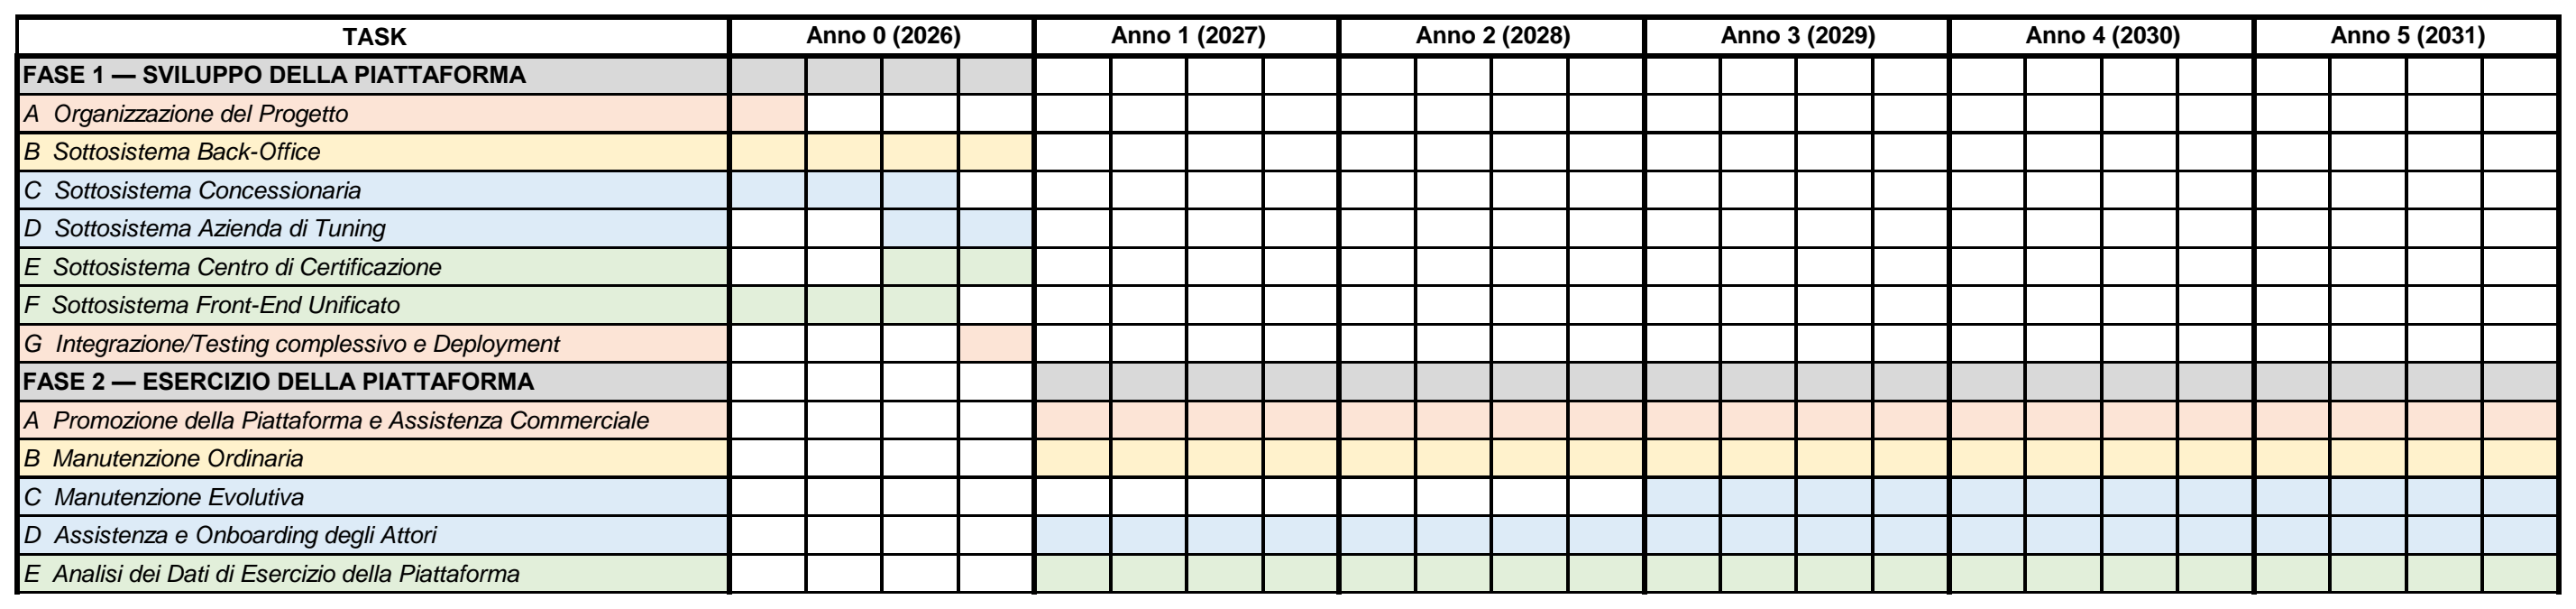
\includegraphics[width=\textwidth]{imgs/gantt/gantt_complessivo.png}
    \caption{Diagramma di GANTT complessivo del progetto}
    \label{fig:gantt-complessivo}
\end{figure}

Le figure professionali impiegate nel progetto, necessarie a garantire la corretta esecuzione delle attività, sono le seguenti:

\begin{itemize}
    \item \textbf{Project Manager (PM)}: si occupa della pianificazione, della gestione e del coordinamento dell'intero progetto, supervisionando le attività di sviluppo, l'allineamento ai requisiti individuati nella modellazione degli use case, il rapporto con gli stakeholder della filiera e il monitoraggio del budget.
    \item \textbf{Software Architect (SA)}: si occupa della progettazione e della definizione dell'architettura a micro-servizi e dell'infrastruttura blockchain, definendo la logica del \textit{chaincode}, le politiche di \textit{endorsement} della rete permissioned e la separazione tra dati on-chain e off-chain.
    \item \textbf{Full Stack Developer (FSD)}: si occupa dello sviluppo completo del software, gestendo sia le interfacce web e mobile destinate agli attori, sia le logiche di back-end e l'interazione con il \textit{chaincode}; assicura inoltre la guida tecnica dei gruppi di lavoro.
    \item \textbf{Full Stack Developer Junior (FSDJ)}: si occupa dello sviluppo dei moduli applicativi di supporto e delle attività di test, lavorando in affiancamento ai Full Stack Developer.
\end{itemize}

Infine, per il progetto si considera che il numero totale di ore di un Anno/Persona (A/P) sia di \textbf{1.752 ore}, equivalenti a 219 giornate lavorative di 8 ore ciascuna. Per semplificare, si assume che le Ore/Persona (O/P) siano distribuite uniformemente nell'arco dell'anno: un Mese/Persona corrisponde quindi a 146 ore e una settimana a 36,5 ore; uno Sprint, della durata di due settimane, equivale pertanto a 73 ore.

\section{Architettura a Componenti della Piattaforma}

L'architettura della piattaforma è ingegnerizzata secondo un modello a \textbf{micro-servizi}, scelta orientata a garantire elevati standard di scalabilità, modularità e manutenibilità del sistema. Tale approccio consente di disaccoppiare le funzionalità di business in componenti software autonomi e indipendenti, ciascuno deputato all'esecuzione di compiti specifici, ottimizzando i cicli di sviluppo e permettendo una scalabilità mirata delle singole risorse.

Al fine di formalizzare la struttura di tale ecosistema tecnologico, la descrizione si avvale di due viste modellistiche basate sullo standard UML (\textit{Unified Modeling Language}):

\begin{itemize}
    \item \textbf{Diagramma dei Componenti}: rappresenta i macro-moduli funzionali, i servizi interni della piattaforma e le relative interfacce di interazione e cooperazione.
    \item \textbf{Diagramma di Distribuzione}: rappresenta la collocazione fisica dei componenti sui nodi di elaborazione e i protocolli di comunicazione impiegati.
\end{itemize}

La Figura~\ref{fig:architettura} illustra la scomposizione logica e i flussi di integrazione dell'architettura complessiva.

\begin{figure}[H]
    \centering
    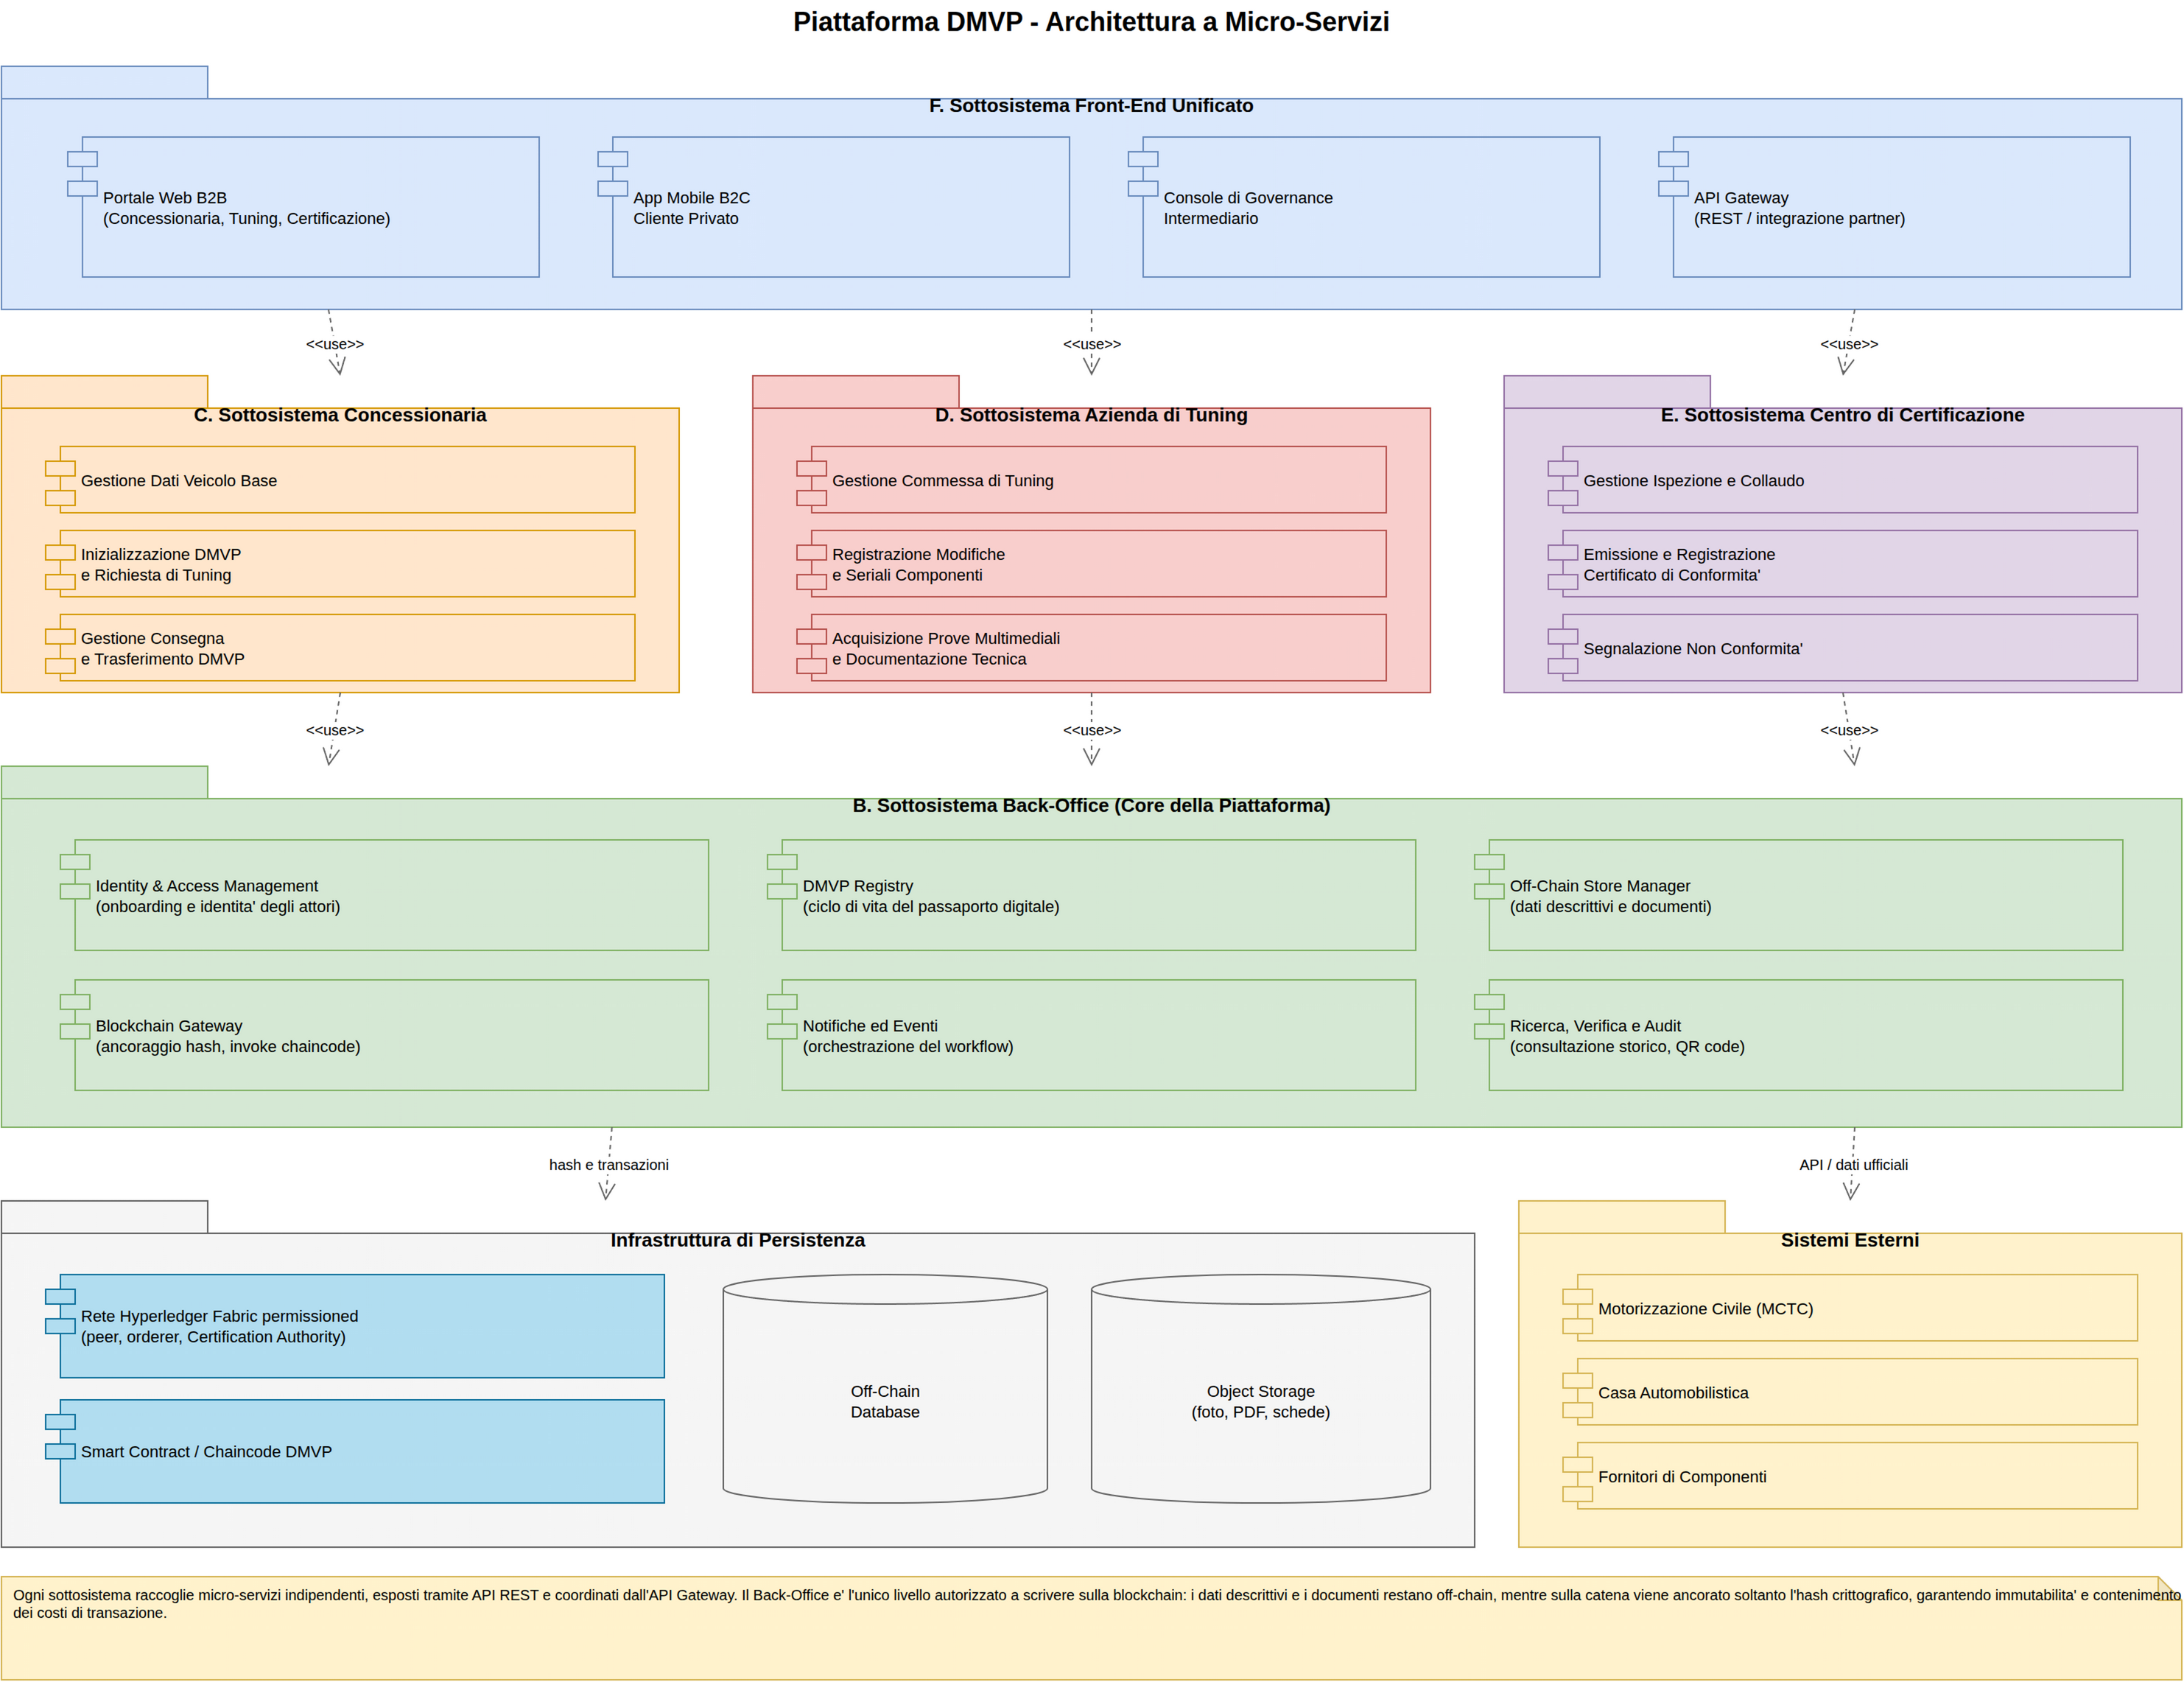
\includegraphics[width=\textwidth]{imgs/projectplan/01_architettura_generale.png}
    \caption{Architettura a micro-servizi della piattaforma DMVP}
    \label{fig:architettura}
\end{figure}

Come si osserva, l'architettura comprende cinque sottosistemi applicativi, poggiati su un'infrastruttura di persistenza ibrida e interfacciati con i sistemi dei partner esterni.

\subsection*{Sottosistema Back-Office}

Il sottosistema Back-Office (Figura~\ref{fig:sub-backoffice}) costituisce il nucleo della piattaforma: comprende tutti i moduli e le logiche computazionali centrali utilizzati in modo trasparente dagli attori, al fine di orchestrare i flussi operativi, gestire la persistenza dei documenti e invocare i metodi esposti dal \textit{chaincode}. Si tratta dell'unico livello autorizzato a scrivere sulla blockchain.

\begin{figure}[H]
    \centering
    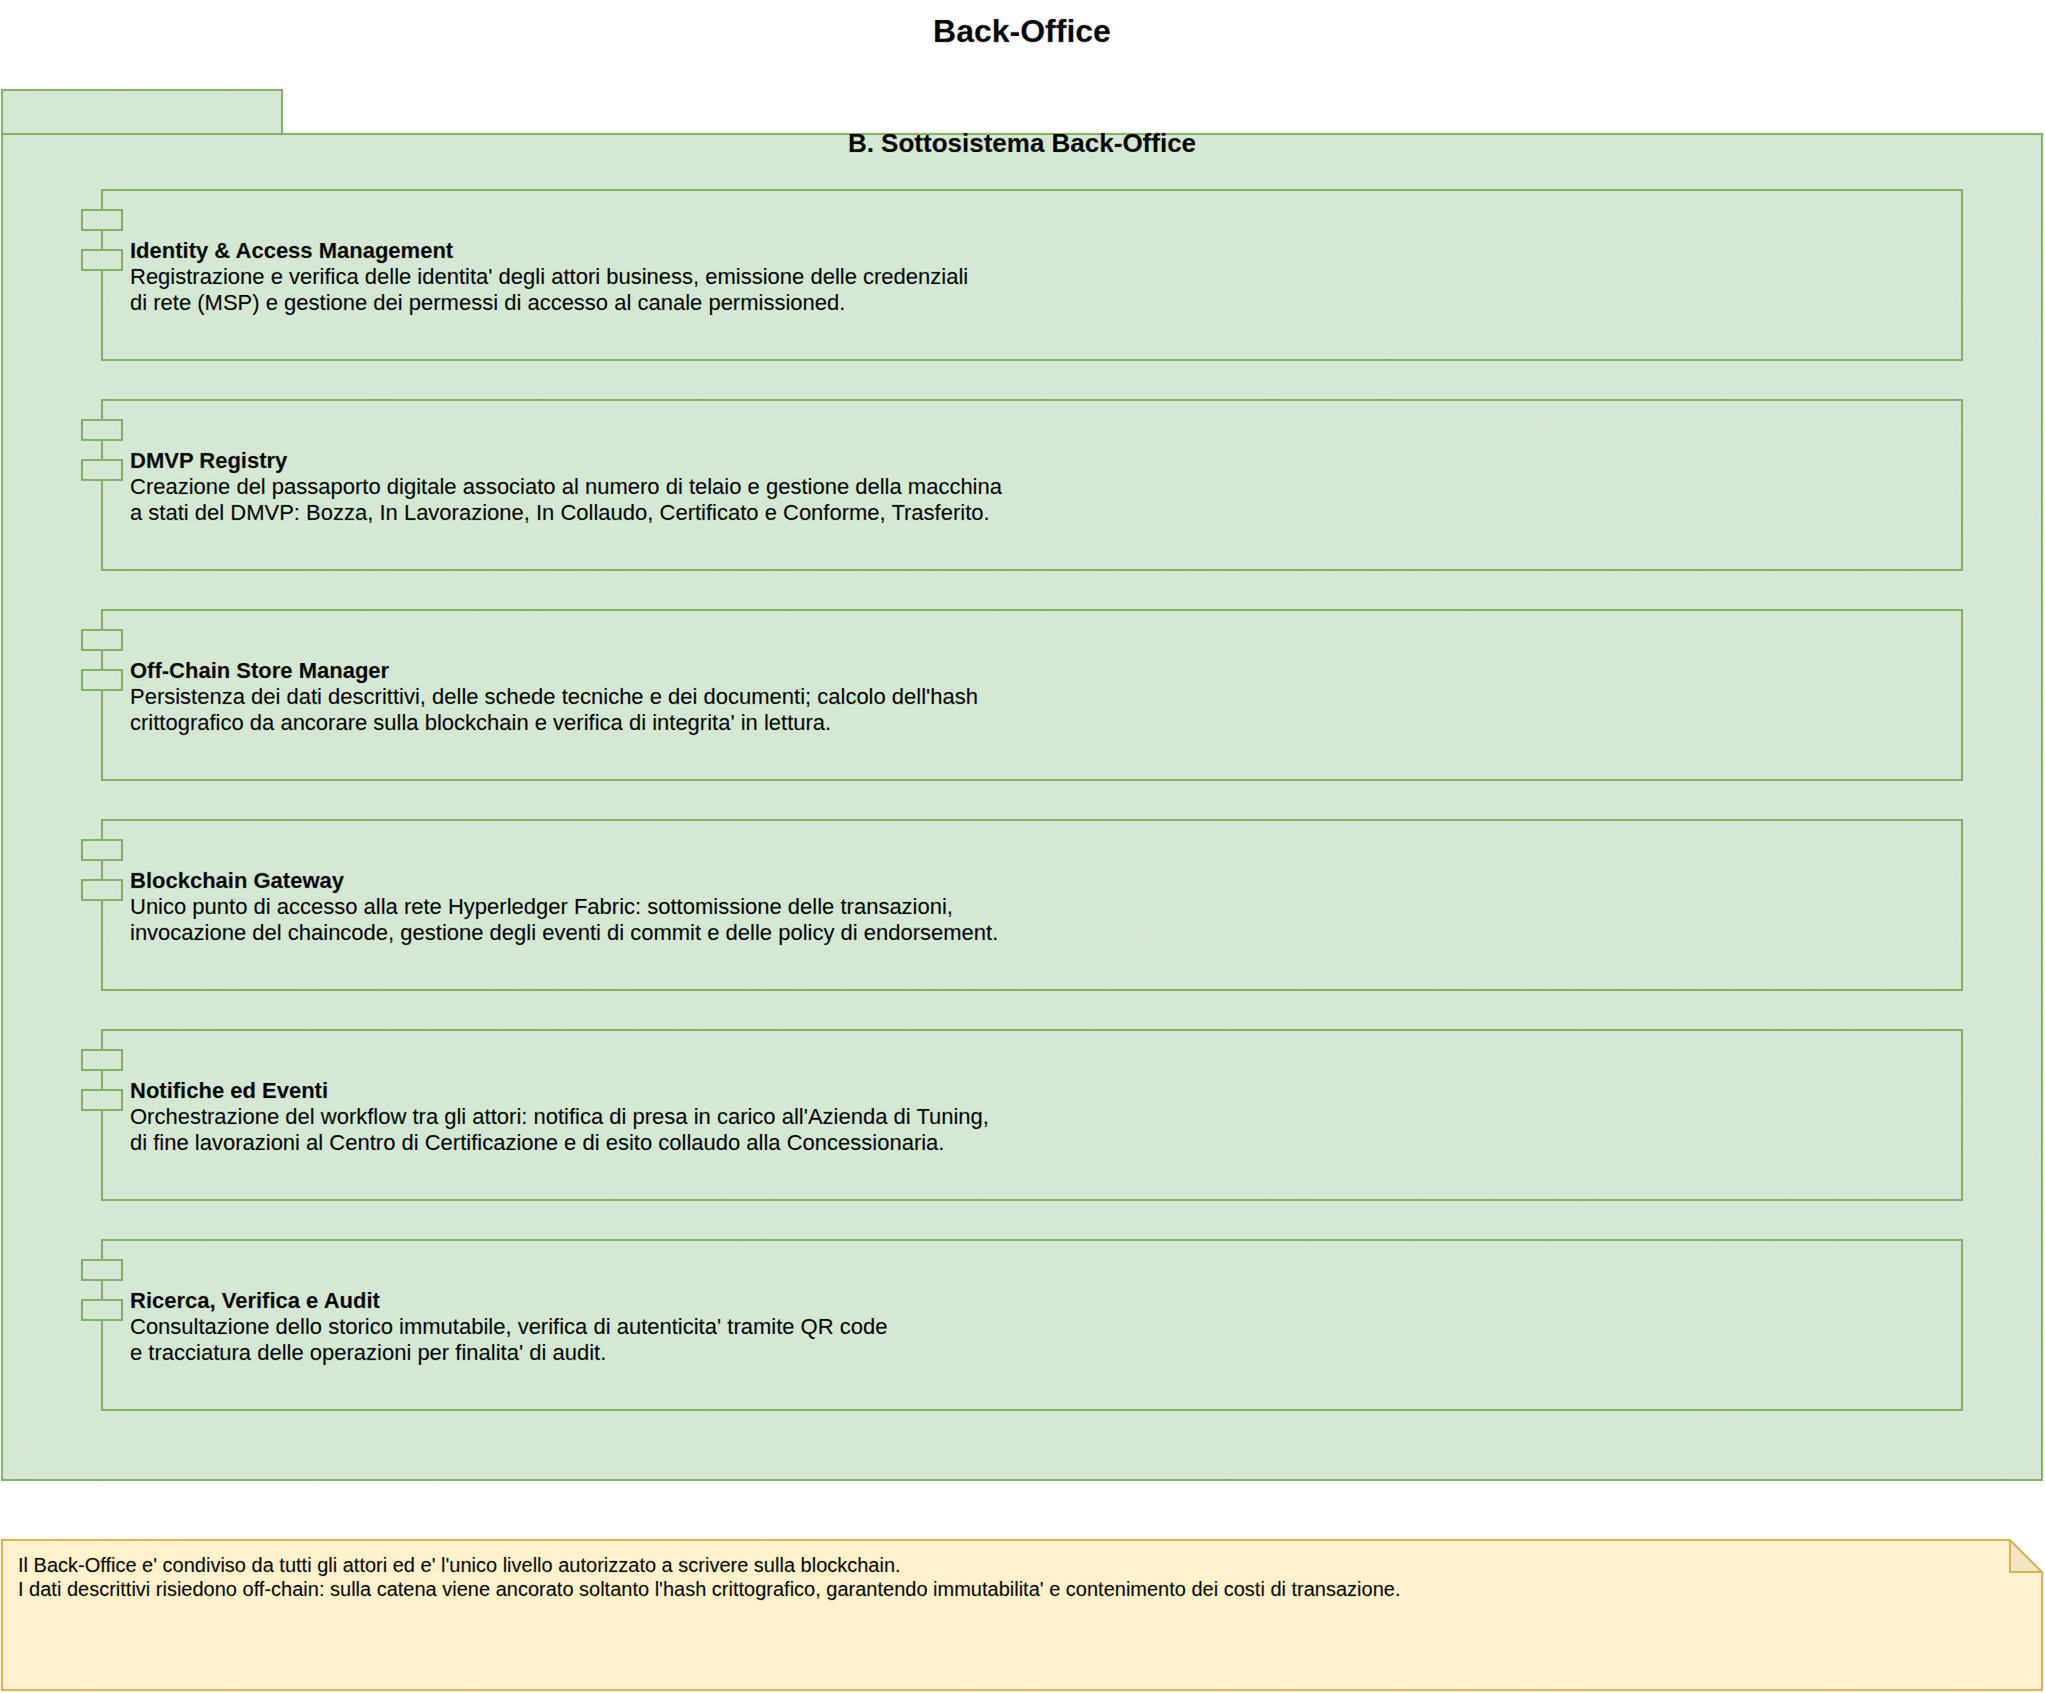
\includegraphics[width=\textwidth]{imgs/projectplan/02_sottosistema_back_office.png}
    \caption{Sottosistema Back-Office}
    \label{fig:sub-backoffice}
\end{figure}

\subsection*{Sottosistema Concessionaria}

Il sottosistema (Figura~\ref{fig:sub-concessionaria}) comprende i moduli dedicati alla Concessionaria, che consentono l'acquisizione e la validazione dei dati identificativi del veicolo originale forniti dalla Casa Automobilistica, la creazione dell'istanza di DMVP e la registrazione delle modifiche commissionate, nonché la gestione della consegna del veicolo omologato e del trasferimento della proprietà del passaporto digitale al Cliente Privato.

\begin{figure}[H]
    \centering
    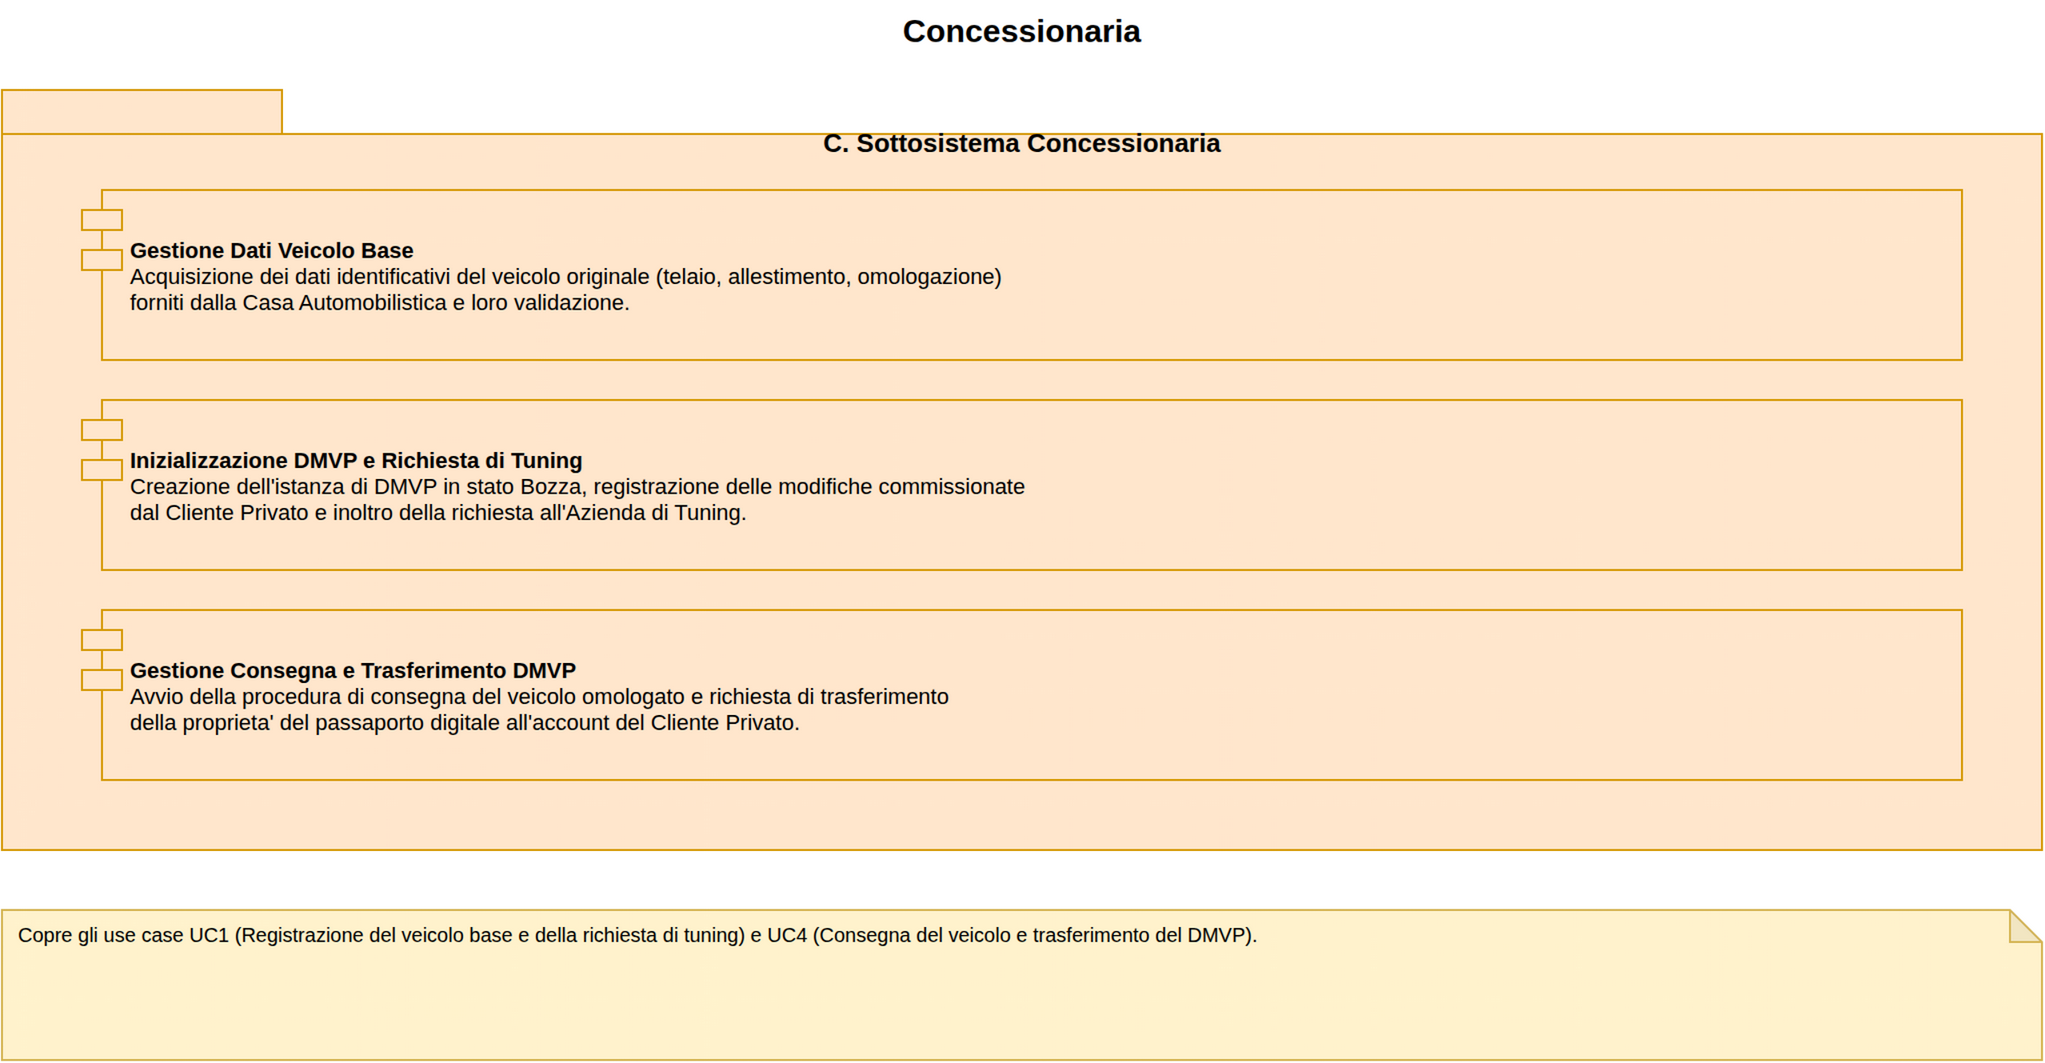
\includegraphics[width=\textwidth]{imgs/projectplan/03_sottosistema_concessionaria.png}
    \caption{Sottosistema Concessionaria}
    \label{fig:sub-concessionaria}
\end{figure}

\subsection*{Sottosistema Azienda di Tuning}

Il sottosistema (Figura~\ref{fig:sub-tuning}) comprende i moduli e le interfacce operative che consentono all'Azienda di Tuning di prendere in carico la commessa, inserire le specifiche tecniche degli interventi e i codici seriali dei componenti installati, e caricare la documentazione tecnica e le prove multimediali a corredo delle lavorazioni eseguite. Rappresenta il cuore operativo della piattaforma, in cui il DMVP viene arricchito in modo immutabile.

\begin{figure}[H]
    \centering
    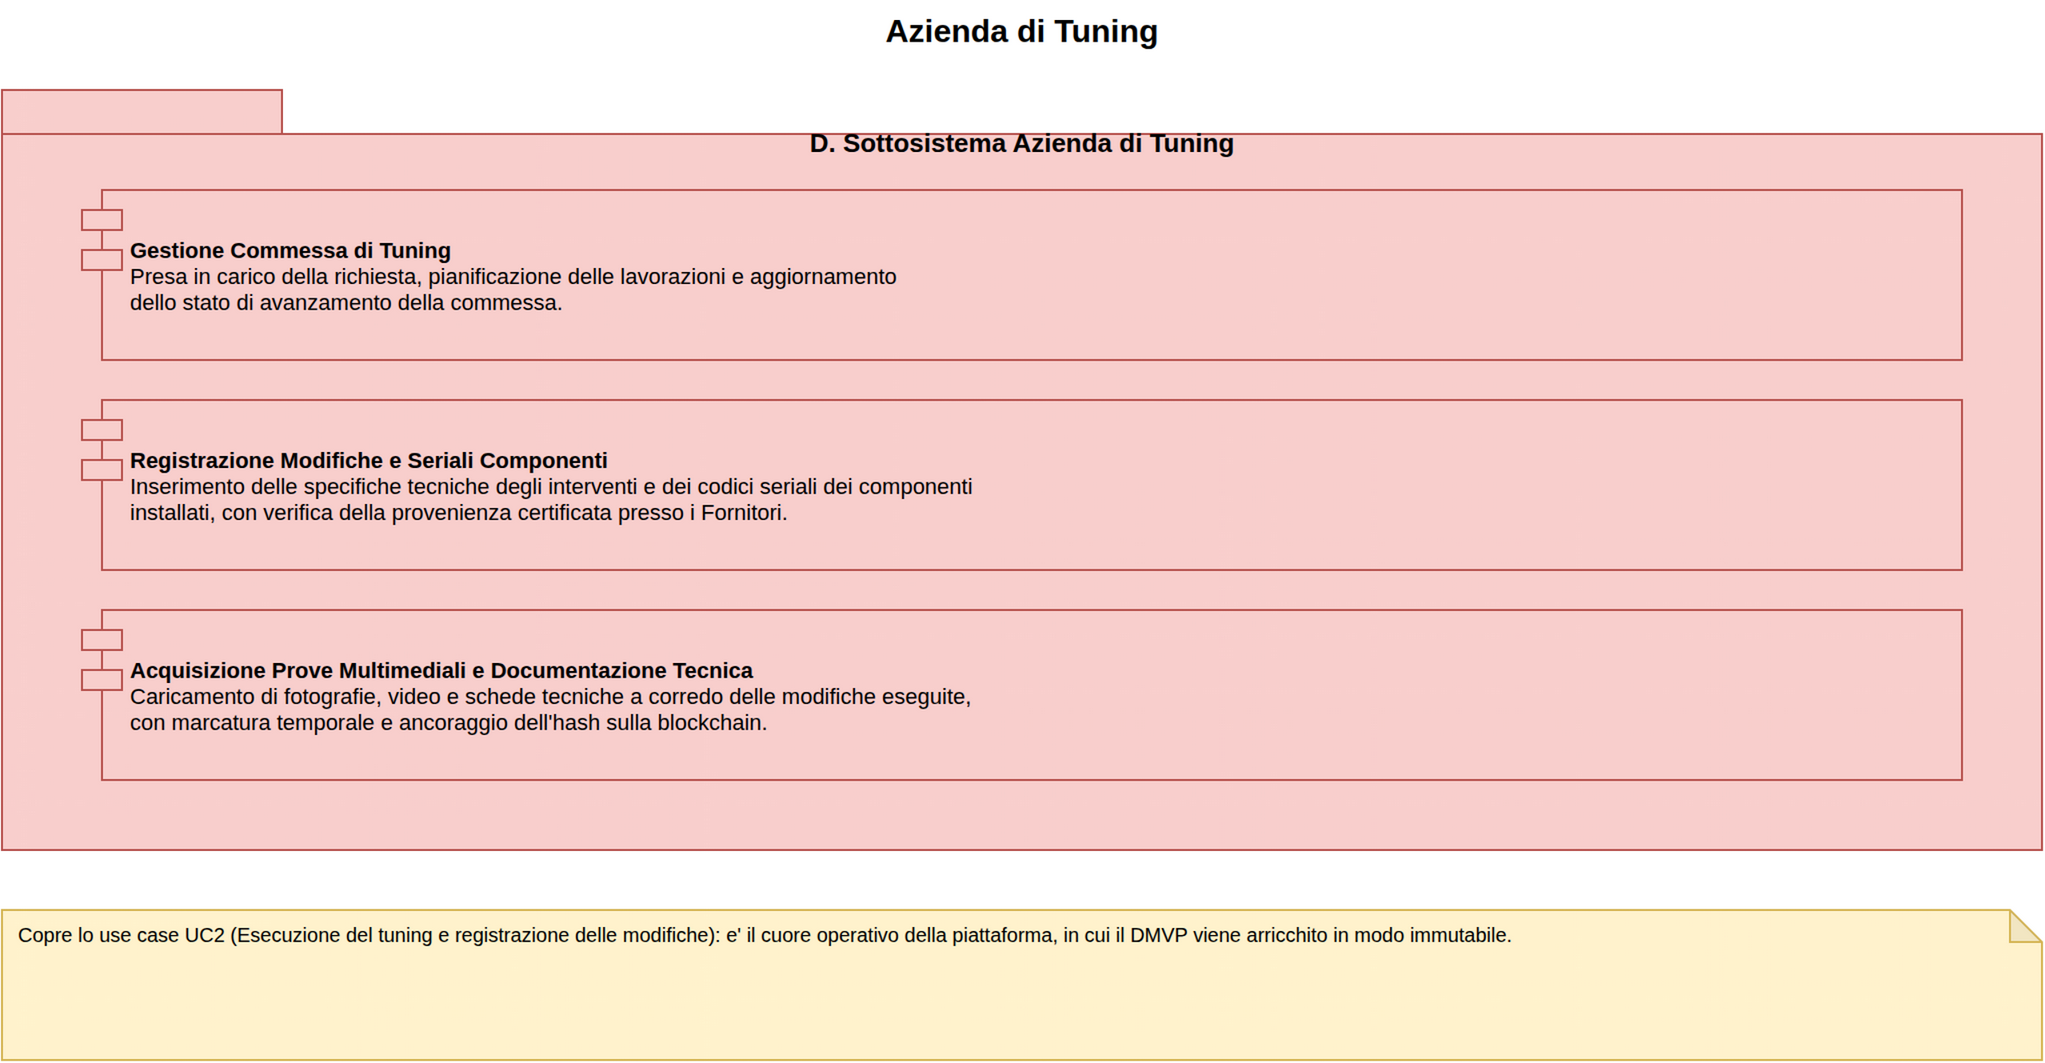
\includegraphics[width=\textwidth]{imgs/projectplan/04_sottosistema_azienda_tuning.png}
    \caption{Sottosistema Azienda di Tuning}
    \label{fig:sub-tuning}
\end{figure}

\subsection*{Sottosistema Centro di Certificazione}

Il sottosistema (Figura~\ref{fig:sub-certificazione}) comprende i moduli destinati al Centro di Certificazione, che permettono la consultazione dello storico immutabile del DMVP, l'esecuzione della checklist normativa e la registrazione degli esiti delle verifiche tecniche, la generazione del certificato digitale firmato con il relativo ancoraggio sulla blockchain e, in caso di esito negativo, la produzione del report di anomalia con reindirizzamento della pratica all'Azienda di Tuning.

\begin{figure}[H]
    \centering
    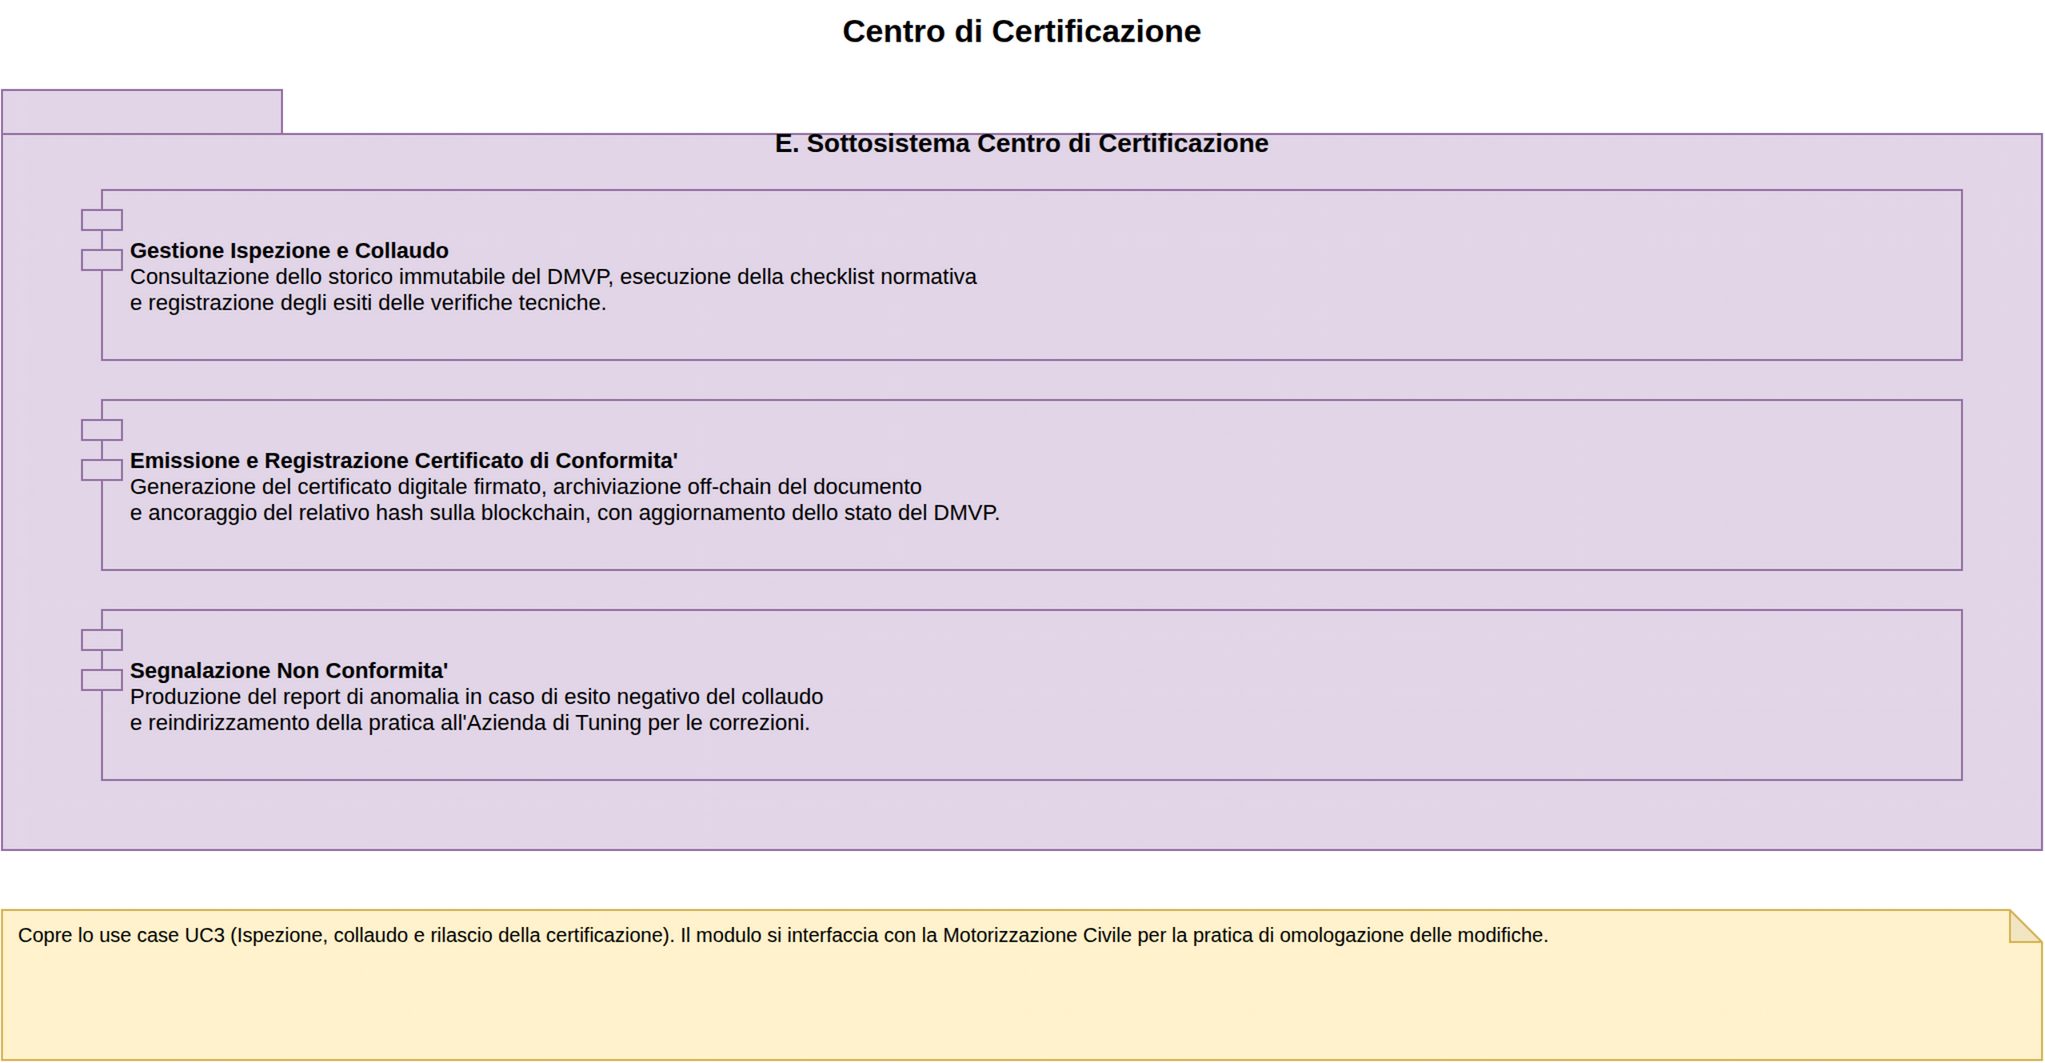
\includegraphics[width=\textwidth]{imgs/projectplan/05_sottosistema_centro_certificazione.png}
    \caption{Sottosistema Centro di Certificazione}
    \label{fig:sub-certificazione}
\end{figure}

\subsection*{Sottosistema Front-End Unificato}

Il sottosistema (Figura~\ref{fig:sub-frontend}) raccoglie l'insieme delle interfacce utente della piattaforma, realizzate come applicazione unica multi-ruolo: la separazione tra utenti B2B e B2C avviene a livello di autenticazione e di profilo autorizzativo. Esso comprende il portale web destinato a Concessionaria, Azienda di Tuning e Centro di Certificazione, l'applicazione mobile per il Cliente Privato, la console di governance dell'Intermediario e l'API Gateway, punto di ingresso unico ai micro-servizi.

\begin{figure}[H]
    \centering
    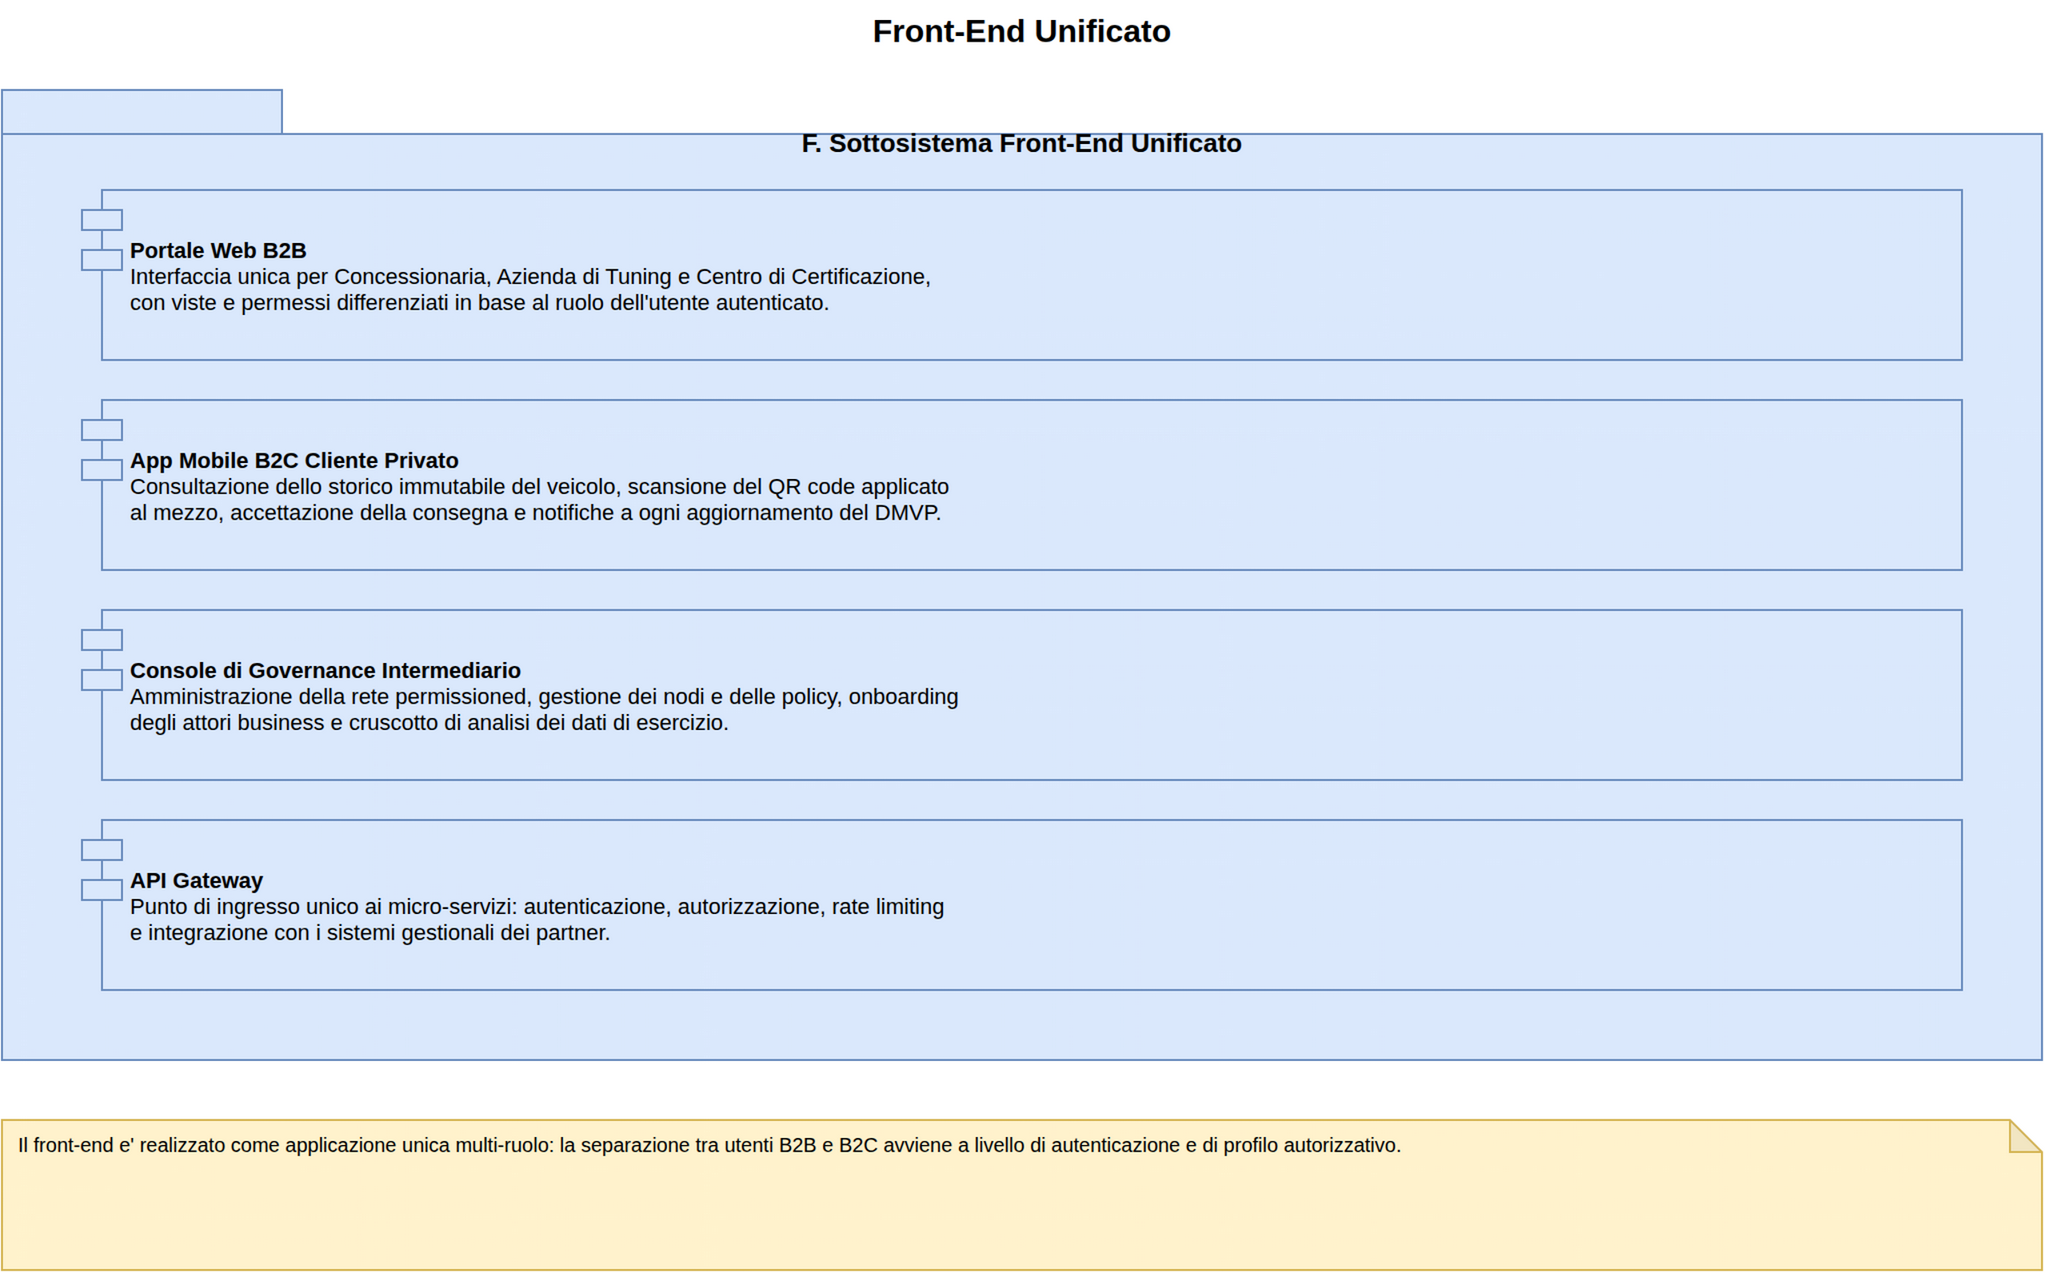
\includegraphics[width=\textwidth]{imgs/projectplan/06_sottosistema_front_end.png}
    \caption{Sottosistema Front-End Unificato}
    \label{fig:sub-frontend}
\end{figure}

\subsection*{Diagramma di Distribuzione}

Il diagramma di distribuzione riportato in Figura~\ref{fig:deployment} illustra la collocazione dei componenti sui nodi di elaborazione. Il cluster applicativo e i nodi della rete permissioned sono ospitati su infrastruttura cloud; ogni organizzazione partecipante mantiene un proprio \textit{peer} con copia del ledger, cosicché nessun attore possa alterare unilateralmente i dati registrati. I documenti e le prove multimediali restano sull'\textit{object storage} off-chain, mentre sulla catena viene scritto soltanto l'hash che ne garantisce l'integrità.

\begin{figure}[H]
    \centering
    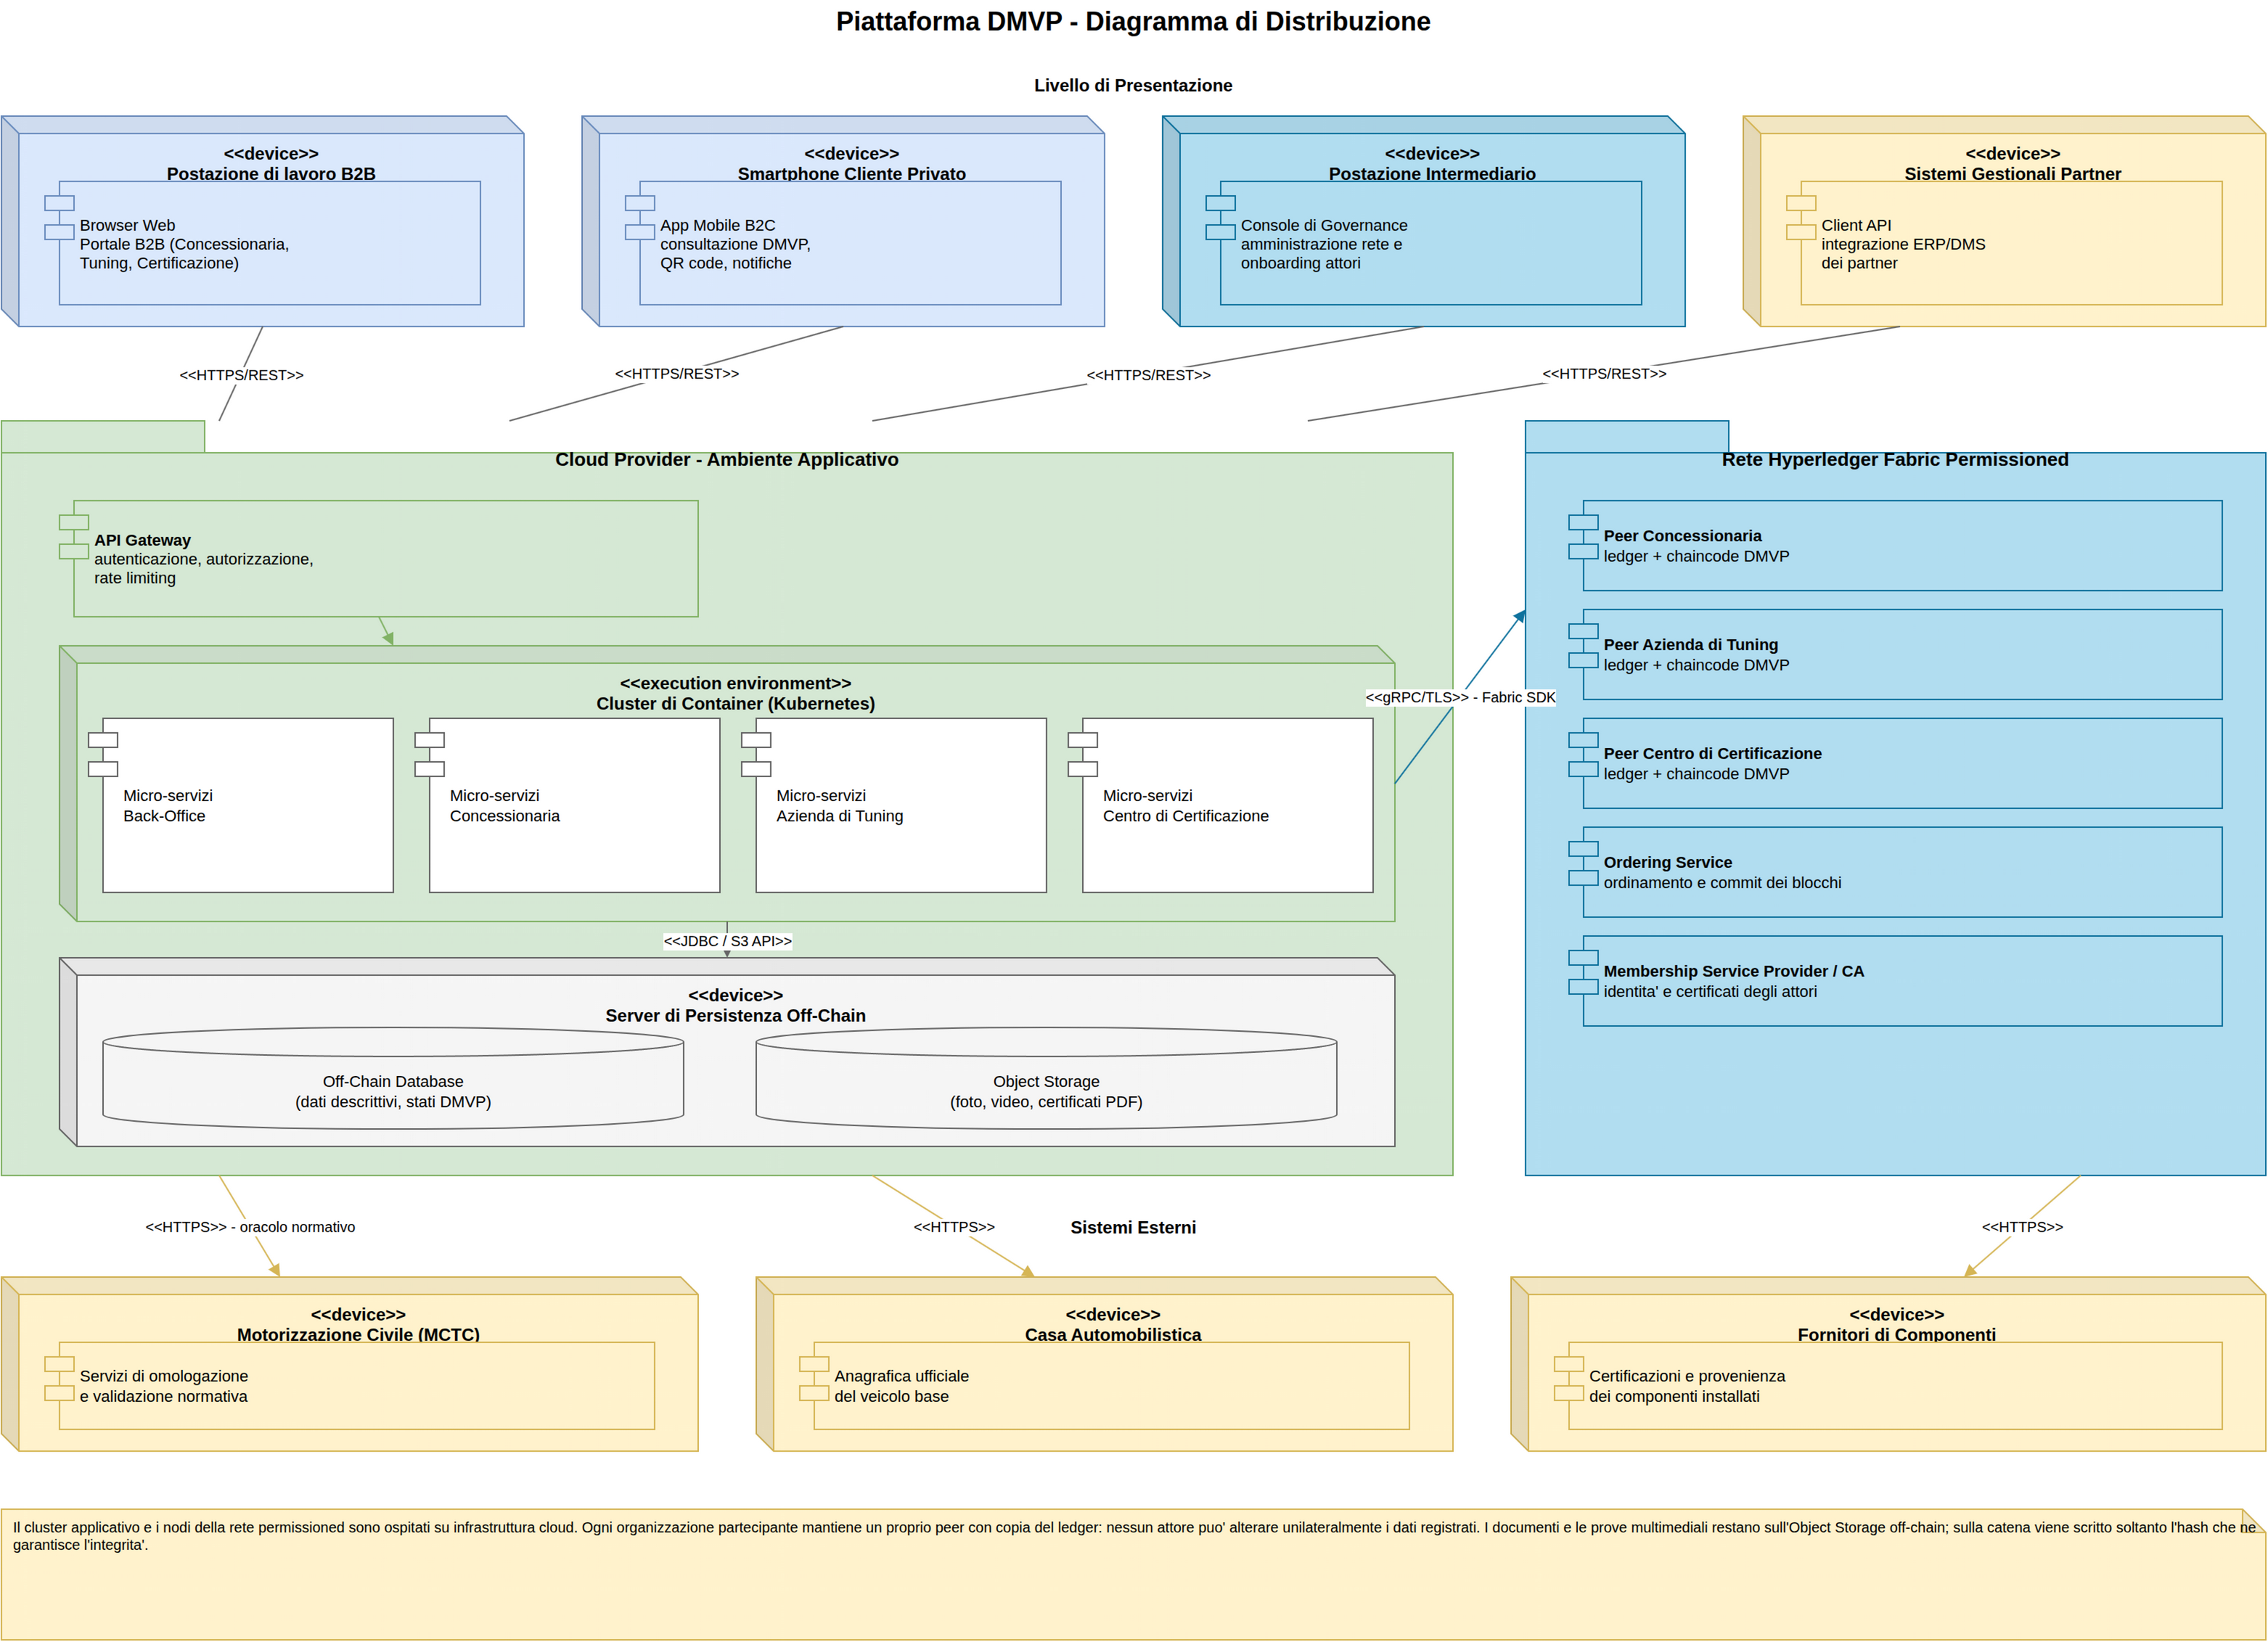
\includegraphics[width=\textwidth]{imgs/projectplan/07_deployment_diagram.png}
    \caption{Diagramma di distribuzione della piattaforma DMVP}
    \label{fig:deployment}
\end{figure}

\section{Ambienti e Tecnologie di Sviluppo}


Per lo strato di registro distribuito viene adottato \textbf{Hyperledger Fabric}, piattaforma blockchain \textit{permissioned} di riferimento per gli scenari consortili. La scelta è motivata dal modello di identità basato su \textit{Membership Service Provider} e Certification Authority, che consente all'Intermediario di verificare preventivamente gli attori ammessi alla rete, e dalle politiche di \textit{endorsement} configurabili, che permettono di stabilire quali organizzazioni debbano validare ciascuna tipologia di transazione. La logica applicativa del passaporto digitale è implementata come \textit{chaincode}, responsabile della registrazione degli hash e della gestione delle transizioni di stato del DMVP.

Per lo sviluppo dei micro-servizi di back-end viene adottato l'ambiente di runtime \textbf{Node.js} accoppiato al framework \textbf{Express}, scelto per la leggerezza, per il modello di I/O asincrono e non bloccante e per l'integrazione nativa con l'SDK di Hyperledger Fabric. Questo stack consente di gestire flussi di richieste ad alta concorrenza riducendo al minimo l'overhead computazionale del server.

Per la gestione dello strato di persistenza, l'architettura adotta un approccio ibrido che separa le informazioni strutturate dai contenuti documentali. Gli stati del DMVP, le anagrafiche degli attori e i metadati delle lavorazioni sono memorizzati in un \textbf{database off-chain}, scelto per la flessibilità dello schema e l'alta velocità di esecuzione delle query. La documentazione voluminosa (fotografie, video, schede tecniche e certificati in formato PDF) è invece delegata a un servizio di \textbf{object storage}, all'interno del quale ciascun oggetto è identificato dalla propria impronta crittografica. Sulla blockchain non vengono quindi allocati i file binari, bensì i soli hash: questa separazione ottimizza le prestazioni del database, contiene i costi di transazione e garantisce al contempo l'inalterabilità delle prove digitali raccolte.

Per il front-end si utilizza \textbf{Flutter}, framework multi-piattaforma basato sul linguaggio Dart, che consente di realizzare con un'unica base di codice sia il portale web B2B sia l'applicazione mobile destinata al Cliente Privato. Flutter si integra efficacemente con le architetture API REST e adotta il pattern MVVM (\textit{Model-View-ViewModel}), in cui il ViewModel gestisce lo stato reattivo dei componenti dell'interfaccia.

L'intero ambiente applicativo è containerizzato mediante \textbf{Docker} e orchestrato tramite \textbf{Kubernetes}, soluzione che garantisce la scalabilità orizzontale dei singoli micro-servizi e l'isolamento dei sottosistemi.

Per lo sviluppo della soluzione vengono infine impiegati i seguenti strumenti:

\begin{itemize}
    \item \textbf{Visual Studio Code}: adottato come ambiente di sviluppo integrato unificato, sia per la componente back-end sia per il front-end in Flutter. La scelta è strategica in quanto garantisce un ambiente leggero, flessibile e altamente personalizzabile, senza rinunciare a strumenti avanzati di refactoring e di completamento intelligente del codice.
    \item \textbf{GitHub}: impiegato come piattaforma di hosting e sistema di controllo di versione distribuito. Semplifica la gestione, il \textit{branching} e la tracciabilità delle modifiche apportate al codice sorgente, consentendo una collaborazione efficiente e parallela tra i membri del team e permettendo di automatizzare le \textit{code review} tramite \textit{Pull Request}.
\end{itemize}

\section{Pianificazione della Prima Fase del Progetto: Sviluppo della Piattaforma}

Lo sviluppo della piattaforma è suddiviso in sette Task principali, ciascuno articolato in diversi sub-task funzionali. Questa scomposizione consente una gestione modulare delle attività e una chiara attribuzione delle responsabilità in base alle competenze del team. La suddivisione dei Task e dei relativi sub-task è dettagliata nella Tabella~\ref{tab:task-fase1}.

\begin{table}[H]
\centering
\small
\makebox[\textwidth][c]{%
\begin{tabular}{clllrr}
\hline
\textbf{Cod.} & \textbf{Task / Sub-task} & \textbf{Gruppo} & \textbf{Periodo} & \textbf{O/P} & \textbf{A/P} \\
\hline
\textbf{A} & \textbf{Organizzazione del Progetto} & Gruppo 0 & & \textbf{3.066} & \textbf{1,75} \\
A1 & Set-Up del Progetto & & sett.\ 1--2 & 438 & 0,25 \\
A2 & Gruppi e Ambienti di Sviluppo & & sett.\ 3--8 & 2.628 & 1,50 \\
\hline
\textbf{B} & \textbf{Sottosistema Back-Office} & Gruppo 1 & & \textbf{5.636} & \textbf{3,22} \\
B1 & Identity \& Access Management e Onboarding & & sett.\ 9--12 & 730 & 0,42 \\
B2 & DMVP Registry e Ciclo di Vita del Passaporto & & sett.\ 13--20 & 1.402 & 0,80 \\
B3 & Off-Chain Store Manager e Blockchain Gateway & & sett.\ 21--30 & 1.752 & 1,00 \\
B4 & Ricerca/Verifica, Notifiche e Integrazione & & sett.\ 31--40 & 1.752 & 1,00 \\
\hline
\textbf{C} & \textbf{Sottosistema Concessionaria} & Gruppo 2 & & \textbf{3.139} & \textbf{1,79} \\
C1 & Gestione Dati Veicolo Base & & sett.\ 9--12 & 511 & 0,29 \\
C2 & Inizializzazione DMVP e Richiesta di Tuning & & sett.\ 13--24 & 1.577 & 0,90 \\
C3 & Gestione Consegna e Trasferimento DMVP & & sett.\ 25--32 & 1.051 & 0,60 \\
\hline
\textbf{D} & \textbf{Sottosistema Azienda di Tuning} & Gruppo 2 & & \textbf{1.051} & \textbf{0,60} \\
D1 & Registrazione Modifiche e Seriali Componenti & & sett.\ 33--36 & 526 & 0,30 \\
D2 & Acquisizione Prove Multimediali e Documentazione & & sett.\ 37--40 & 526 & 0,30 \\
\hline
\textbf{E} & \textbf{Sottosistema Centro di Certificazione} & Gruppo 3 & & \textbf{1.051} & \textbf{0,60} \\
E1 & Gestione Ispezione e Collaudo & & sett.\ 33--36 & 526 & 0,30 \\
E2 & Emissione e Registrazione del Certificato & & sett.\ 37--40 & 526 & 0,30 \\
\hline
\textbf{F} & \textbf{Sottosistema Front-End Unificato} & Gruppo 3 & & \textbf{3.139} & \textbf{1,79} \\
F1 & Portale Web B2B & & sett.\ 9--18 & 1.299 & 0,74 \\
F2 & App Mobile B2C Cliente Privato & & sett.\ 19--26 & 1.051 & 0,60 \\
F3 & Console di Governance Intermediario e Analytics & & sett.\ 27--32 & 788 & 0,45 \\
\hline
\textbf{G} & \textbf{Integrazione/Testing complessivo e Deployment} & Gruppo 0 & & \textbf{3.504} & \textbf{2,00} \\
G1 & Integrazione/Testing complessivo & & sett.\ 41--46 & 2.628 & 1,50 \\
G2 & Deployment & & sett.\ 47--48 & 876 & 0,50 \\
\hline
& \textbf{TOTALE FASE 1} & & & \textbf{20.586} & \textbf{11,75} \\
\hline
\end{tabular}}
\caption{Task e sub-task della Prima Fase}
\label{tab:task-fase1}
\end{table}

Nella pianificazione del progetto si fa riferimento alla metodologia \textbf{Agile}, e in particolare a \textbf{Scrum}, framework di processo iterativo e incrementale ampiamente consolidato nell'ingegneria del software.

Scrum prevede di suddividere il ciclo di vita dello sviluppo in periodi di lavoro brevi e ben definiti, noti come \textbf{Sprint}, al termine dei quali viene rilasciato un incremento di software funzionante, testato e potenzialmente rilasciabile. Questo approccio consente di definire in dettaglio le attività a breve termine e include una serie di cerimonie progettate per monitorare costantemente l'avanzamento del lavoro, minimizzare i rischi operativi e favorire momenti di revisione e miglioramento continuo. Nel presente progetto la durata di uno Sprint è fissata in \textbf{due settimane}, pari a 73 O/P per risorsa a tempo pieno.

Un Team Scrum è composto da tre figure chiave:

\begin{itemize}
    \item \textbf{Product Owner}: rappresenta la voce degli stakeholder e dei clienti finali, assicurandosi che il team sviluppi soluzioni orientate al valore di business e ordinando il \textit{Product Backlog} in base alle priorità strategiche. Nel presente progetto tale ruolo è assunto dal Project Manager.
    \item \textbf{Development Team}: il gruppo cross-funzionale di professionisti che si occupa materialmente della progettazione, dell'implementazione e del testing del software.
    \item \textbf{Scrum Master}: agisce come leader al servizio del team, con il compito di diffondere la cultura Agile, ottimizzare i processi interni e rimuovere tempestivamente gli impedimenti che potrebbero rallentare il raggiungimento degli obiettivi di Sprint. Tale ruolo è assunto dal Software Architect.
\end{itemize}

Ogni Sprint inizia con una riunione di \textit{Sprint Planning}, durante la quale vengono determinati gli obiettivi del ciclo e stimate le risorse necessarie per completarli, estraendole dal backlog. Al termine di ogni Sprint, durante la \textit{Sprint Review}, il team consegna e dimostra una versione operativa del prodotto, procedendo poi alla \textit{Sprint Retrospective} per analizzare e ottimizzare i processi di lavoro interni.

Per quanto concerne la pianificazione delle risorse umane impiegate nella prima fase, si considera l'impiego delle seguenti figure professionali:

\begin{itemize}
    \item \textbf{Un Project Manager (PM)}, coinvolto in tutte le macro-attività del ciclo di vita con il ruolo metodologico di Product Owner, per garantire la corrispondenza dei moduli sviluppati alle specifiche di business individuate nella modellazione.
    \item \textbf{Un Software Architect (SA)}, presente trasversalmente in tutti i task operativi con il ruolo di Scrum Master, per supervisionare la coerenza tecnica dell'architettura a micro-servizi e della componente blockchain e per guidare l'intero team di sviluppo.
    \item \textbf{Quattro Full Stack Developer (FSD)}, distribuiti all'interno dei gruppi di lavoro e responsabili primari dell'implementazione delle logiche computazionali del Back-Office, della scrittura del chaincode e dell'integrazione con la rete permissioned.
    \item \textbf{Sei Full Stack Developer Junior (FSDJ)}, distribuiti nei vari team e focalizzati sulla realizzazione dei moduli applicativi di supporto e delle interfacce in Flutter, lavorando in sinergia con il back-end.
\end{itemize}

I gruppi di lavoro individuati sono quattro e vengono riassunti in Figura~\ref{fig:gruppi-fase1} e nella Tabella~\ref{tab:gruppi-fase1}.

\begin{figure}[H]
    \centering
    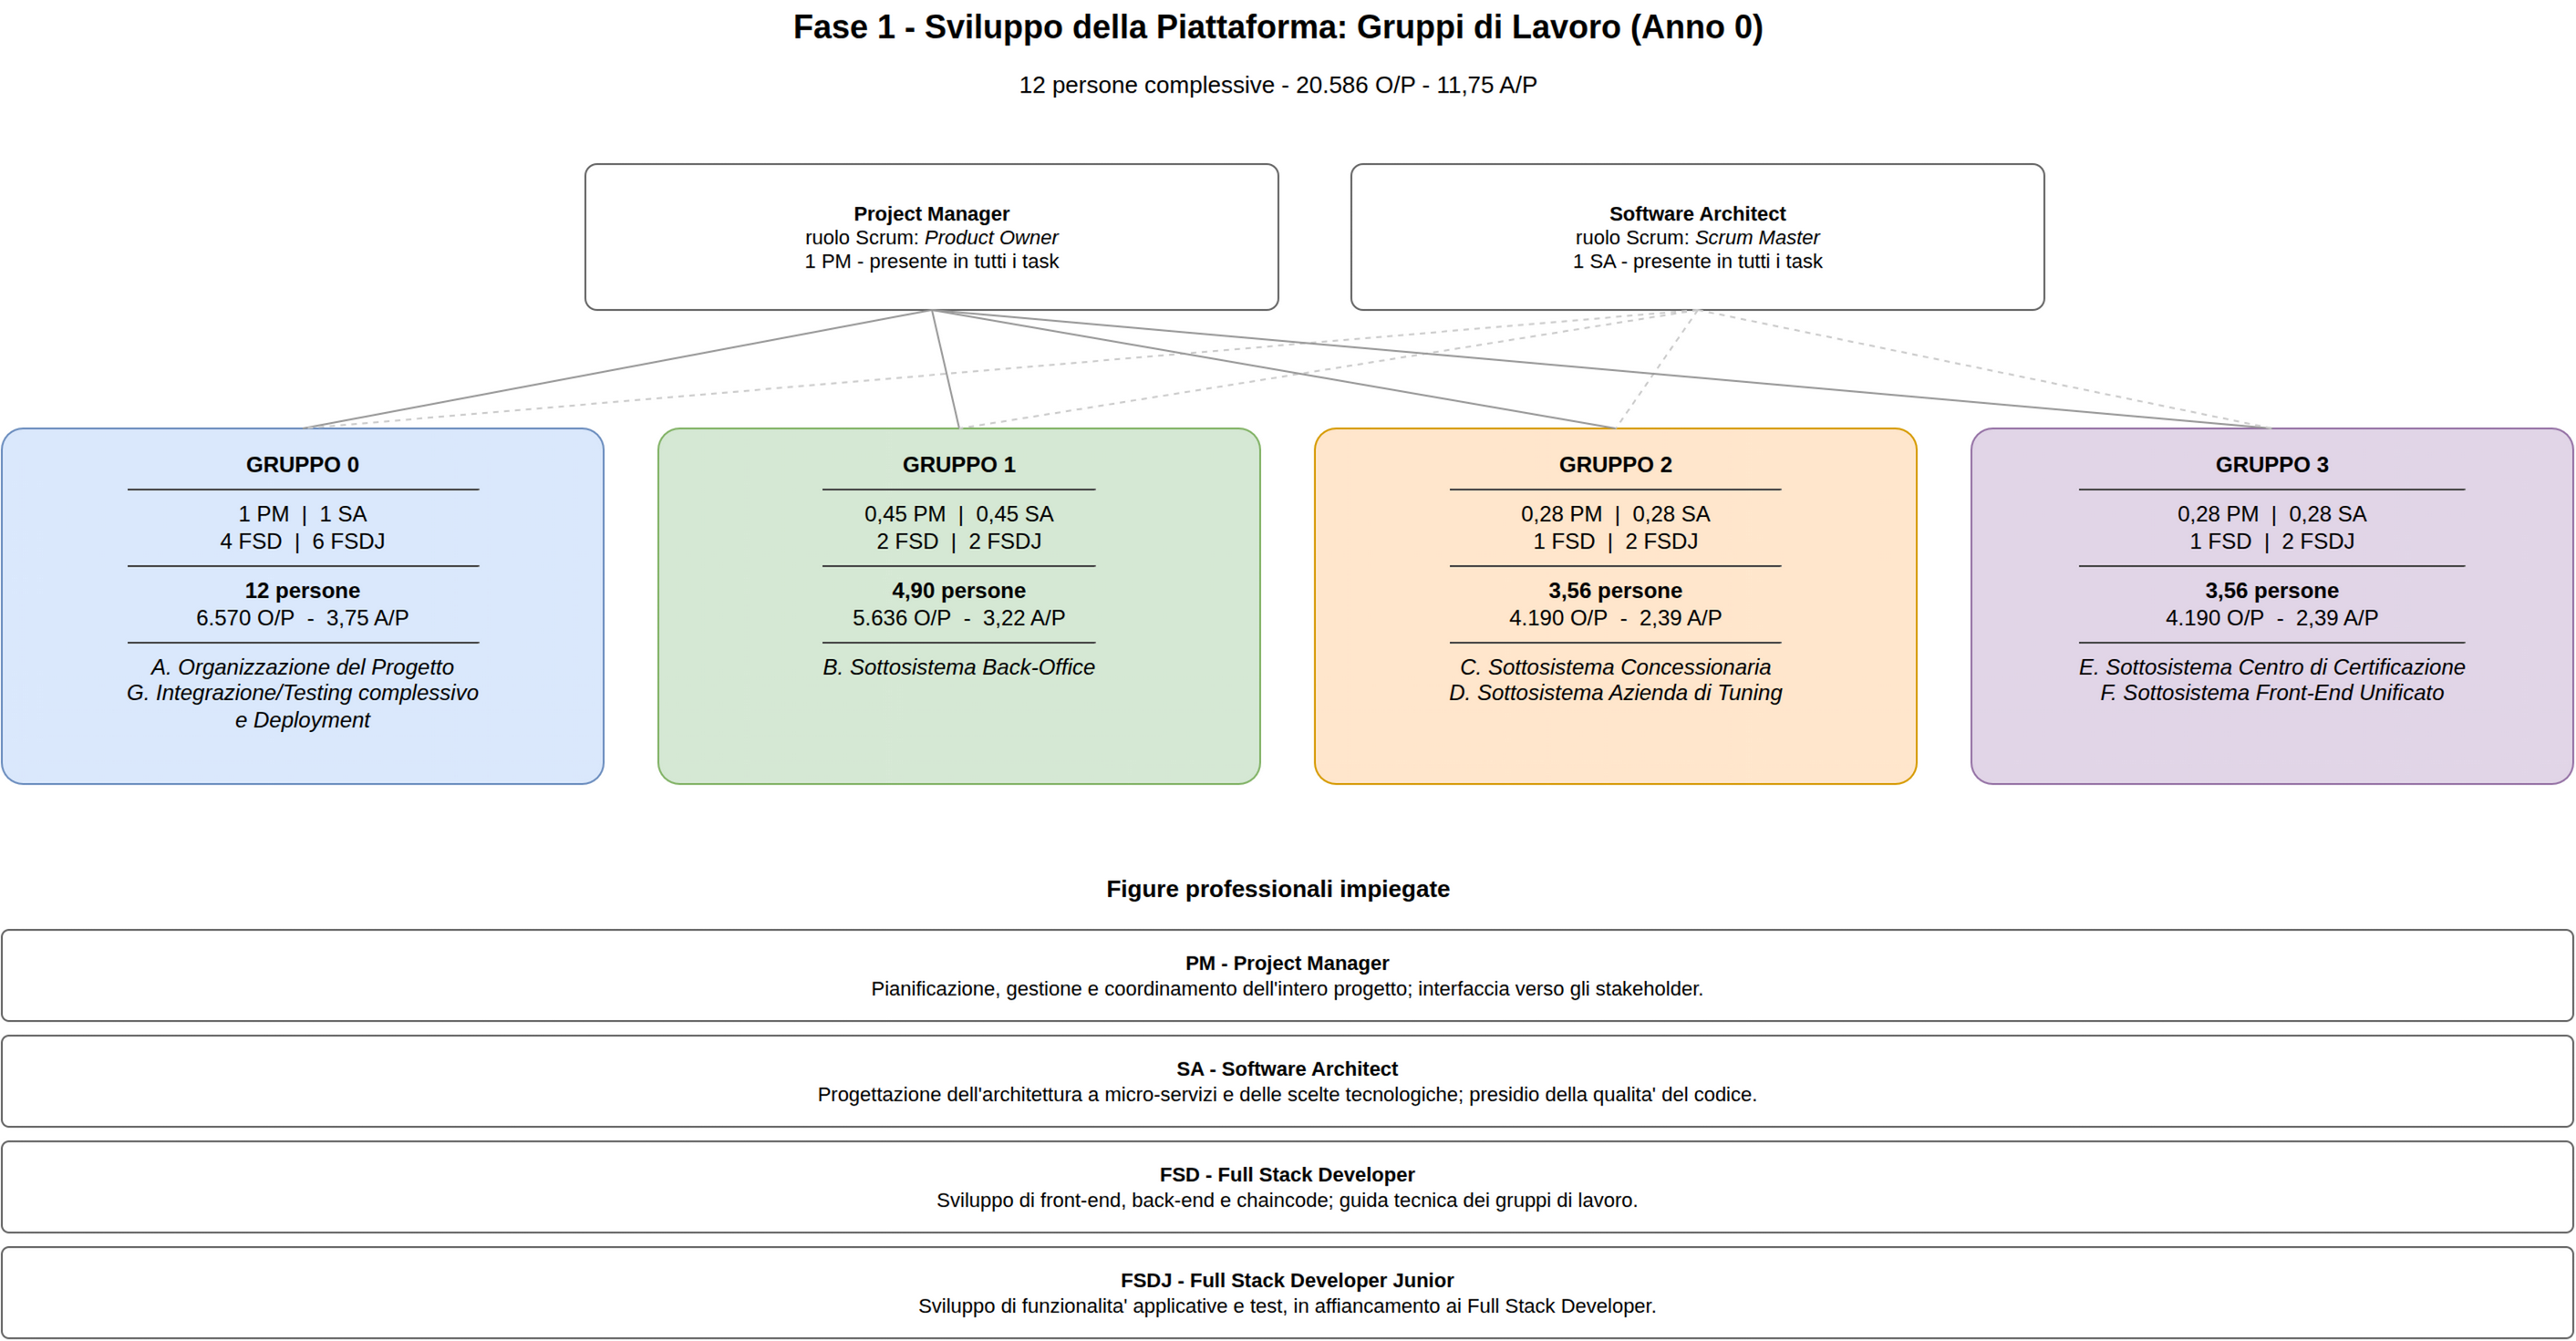
\includegraphics[width=\textwidth]{imgs/projectplan/08_gruppi_fase1.png}
    \caption{Gruppi di lavoro della Fase 1}
    \label{fig:gruppi-fase1}
\end{figure}

\begin{table}[H]
\centering
\small
\makebox[\textwidth][c]{%
\begin{tabular}{llll rr}
\hline
\textbf{Gruppo} & \textbf{Persone} & \textbf{Tipologia} & \textbf{Task} & \textbf{O/P} & \textbf{A/P} \\
\hline
Gruppo 0 & 12,00 & 1 PM, 1 SA, 4 FSD, 6 FSDJ & A, G & 6.570 & 3,75 \\
Gruppo 1 & 4,90 & 0,45 PM, 0,45 SA, 2 FSD, 2 FSDJ & B & 5.636 & 3,22 \\
Gruppo 2 & 3,56 & 0,28 PM, 0,28 SA, 1 FSD, 2 FSDJ & C, D & 4.190 & 2,39 \\
Gruppo 3 & 3,56 & 0,28 PM, 0,28 SA, 1 FSD, 2 FSDJ & E, F & 4.190 & 2,39 \\
\hline
\textbf{TOTALE} & \textbf{12} & 1 PM, 1 SA, 4 FSD, 6 FSDJ & A--G & \textbf{20.586} & \textbf{11,75} \\
\hline
\end{tabular}}
\caption{Composizione e impegno dei gruppi di lavoro della Fase 1}
\label{tab:gruppi-fase1}
\end{table}

I Gruppi 1, 2 e 3 lavorano in parallelo sui rispettivi sottosistemi, mentre il Gruppo 0 coincide con l'intero organico ed è impegnato nelle attività iniziali di organizzazione e nelle attività finali di integrazione, testing e deployment. Il Project Manager e il Software Architect sono ripartiti tra i gruppi in quota proporzionale all'impegno richiesto da ciascun sottosistema.

Il diagramma di GANTT della prima fase, articolato sulle 48 settimane dell'Anno 0 --- raggruppate nei dodici mesi di calendario e scandite in Sprint di due settimane ciascuno --- è riportato in Figura~\ref{fig:gantt-fase1}.

\begin{figure}[H]
    \centering
    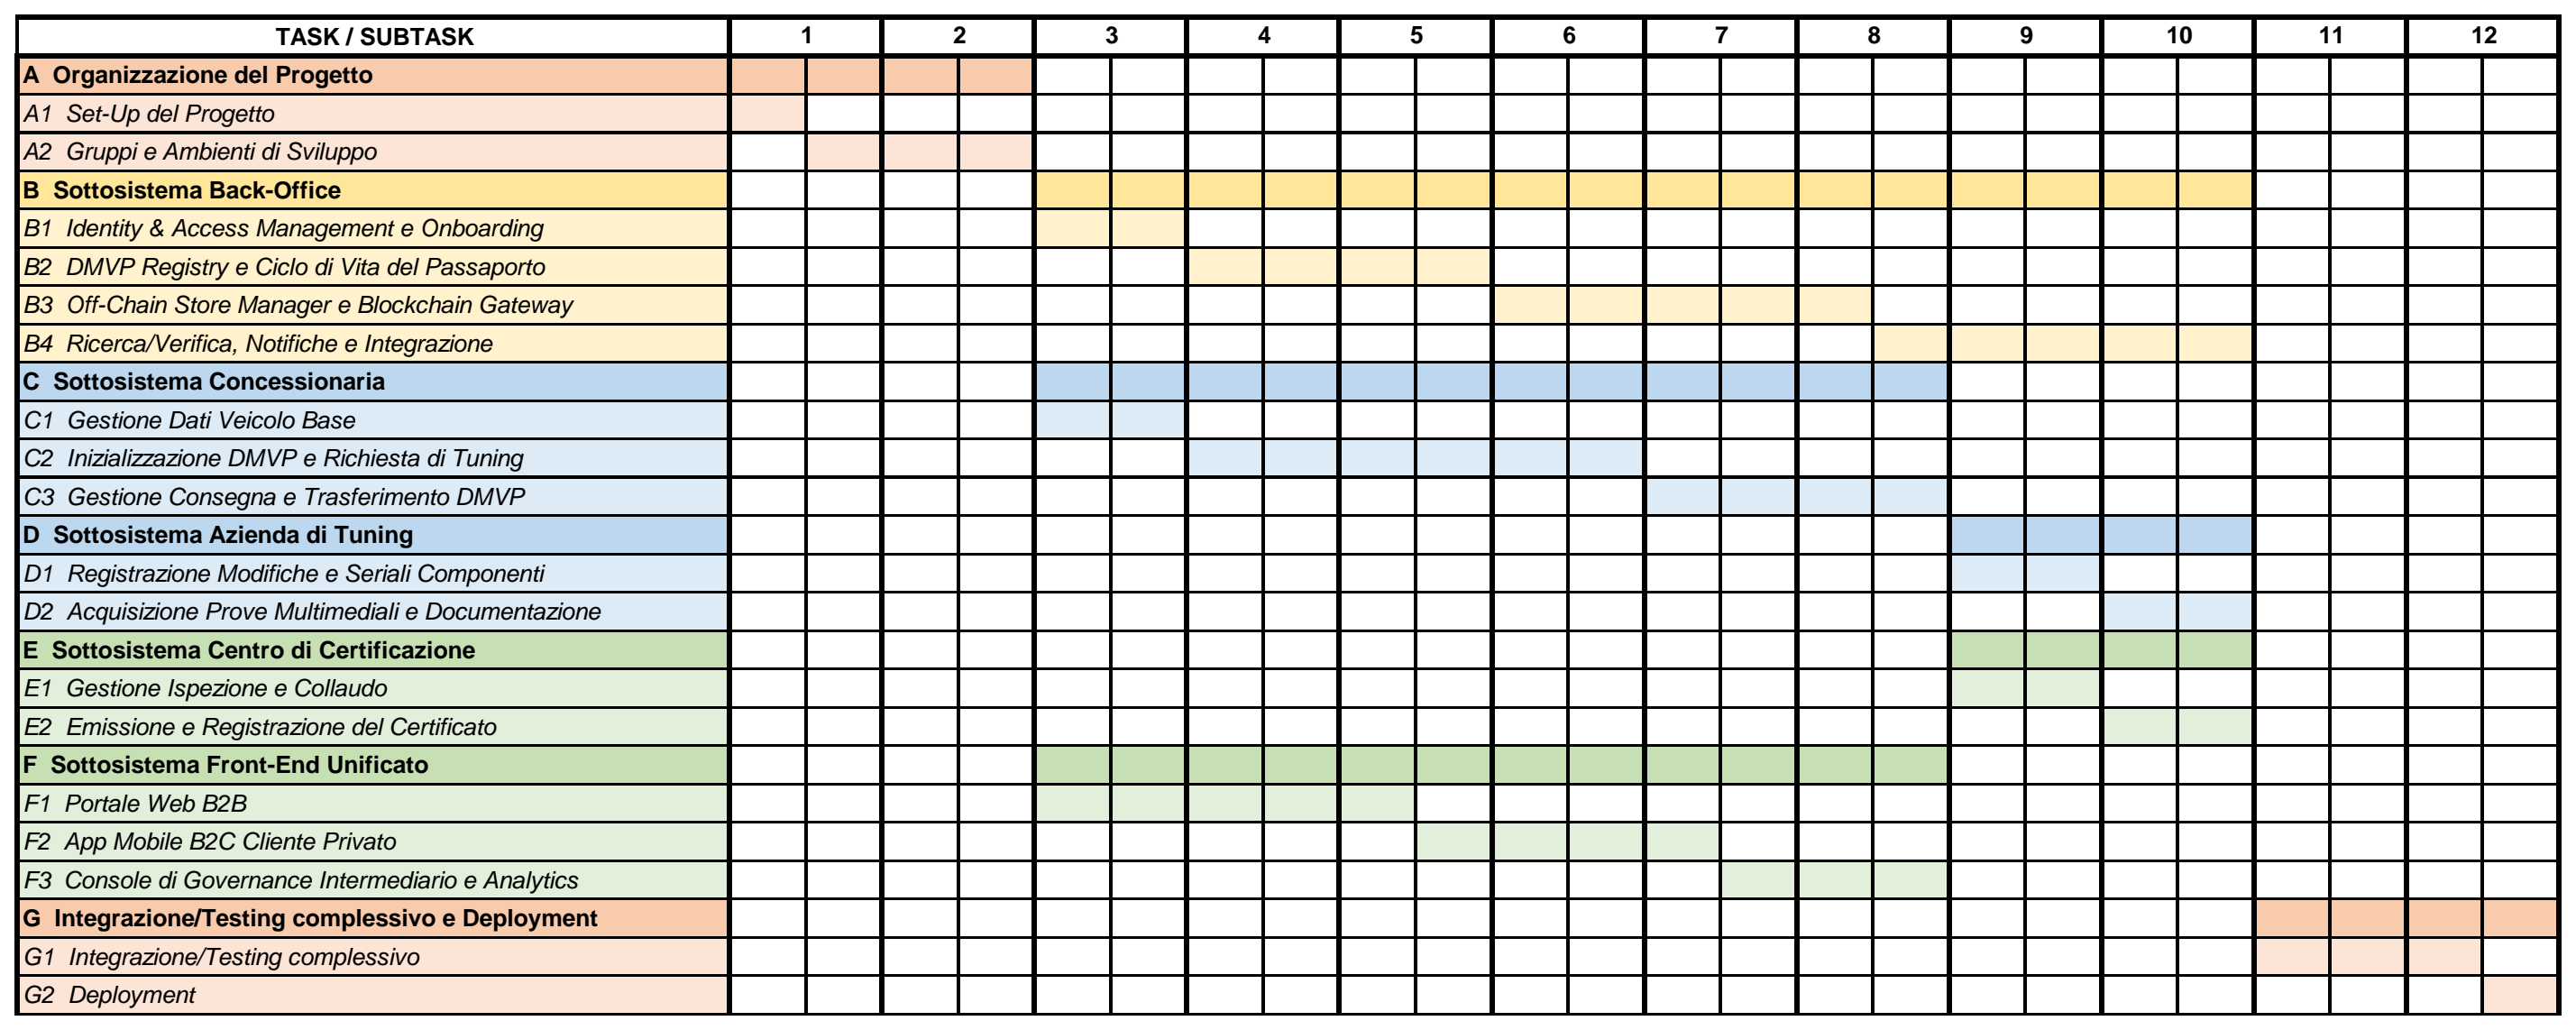
\includegraphics[width=\textwidth]{imgs/gantt/gantt_fase1/gantt_fase1.png}
    \caption{Diagramma di GANTT della Fase 1}
    \label{fig:gantt-fase1}
\end{figure}

Le diverse tipologie di risorsa vengono impegnate all'interno dei vari task come mostrato nelle Figure~\ref{fig:impegno-pm-fase1}, \ref{fig:impegno-sa-fase1}, \ref{fig:impegno-fsd-fase1}, \ref{fig:impegno-fsdj-fase1} e~\ref{fig:impegno-totale-fase1}. Si osservi che nelle prime due settimane, dedicate al solo Set-Up del Progetto, risultano operativi il Project Manager, il Software Architect e i quattro Full Stack Developer, mentre i sei Full Stack Developer Junior vengono inseriti a partire dalla terza settimana, contestualmente alla costituzione dei gruppi e alla predisposizione degli ambienti di sviluppo.

\begin{figure}[H]
    \centering
    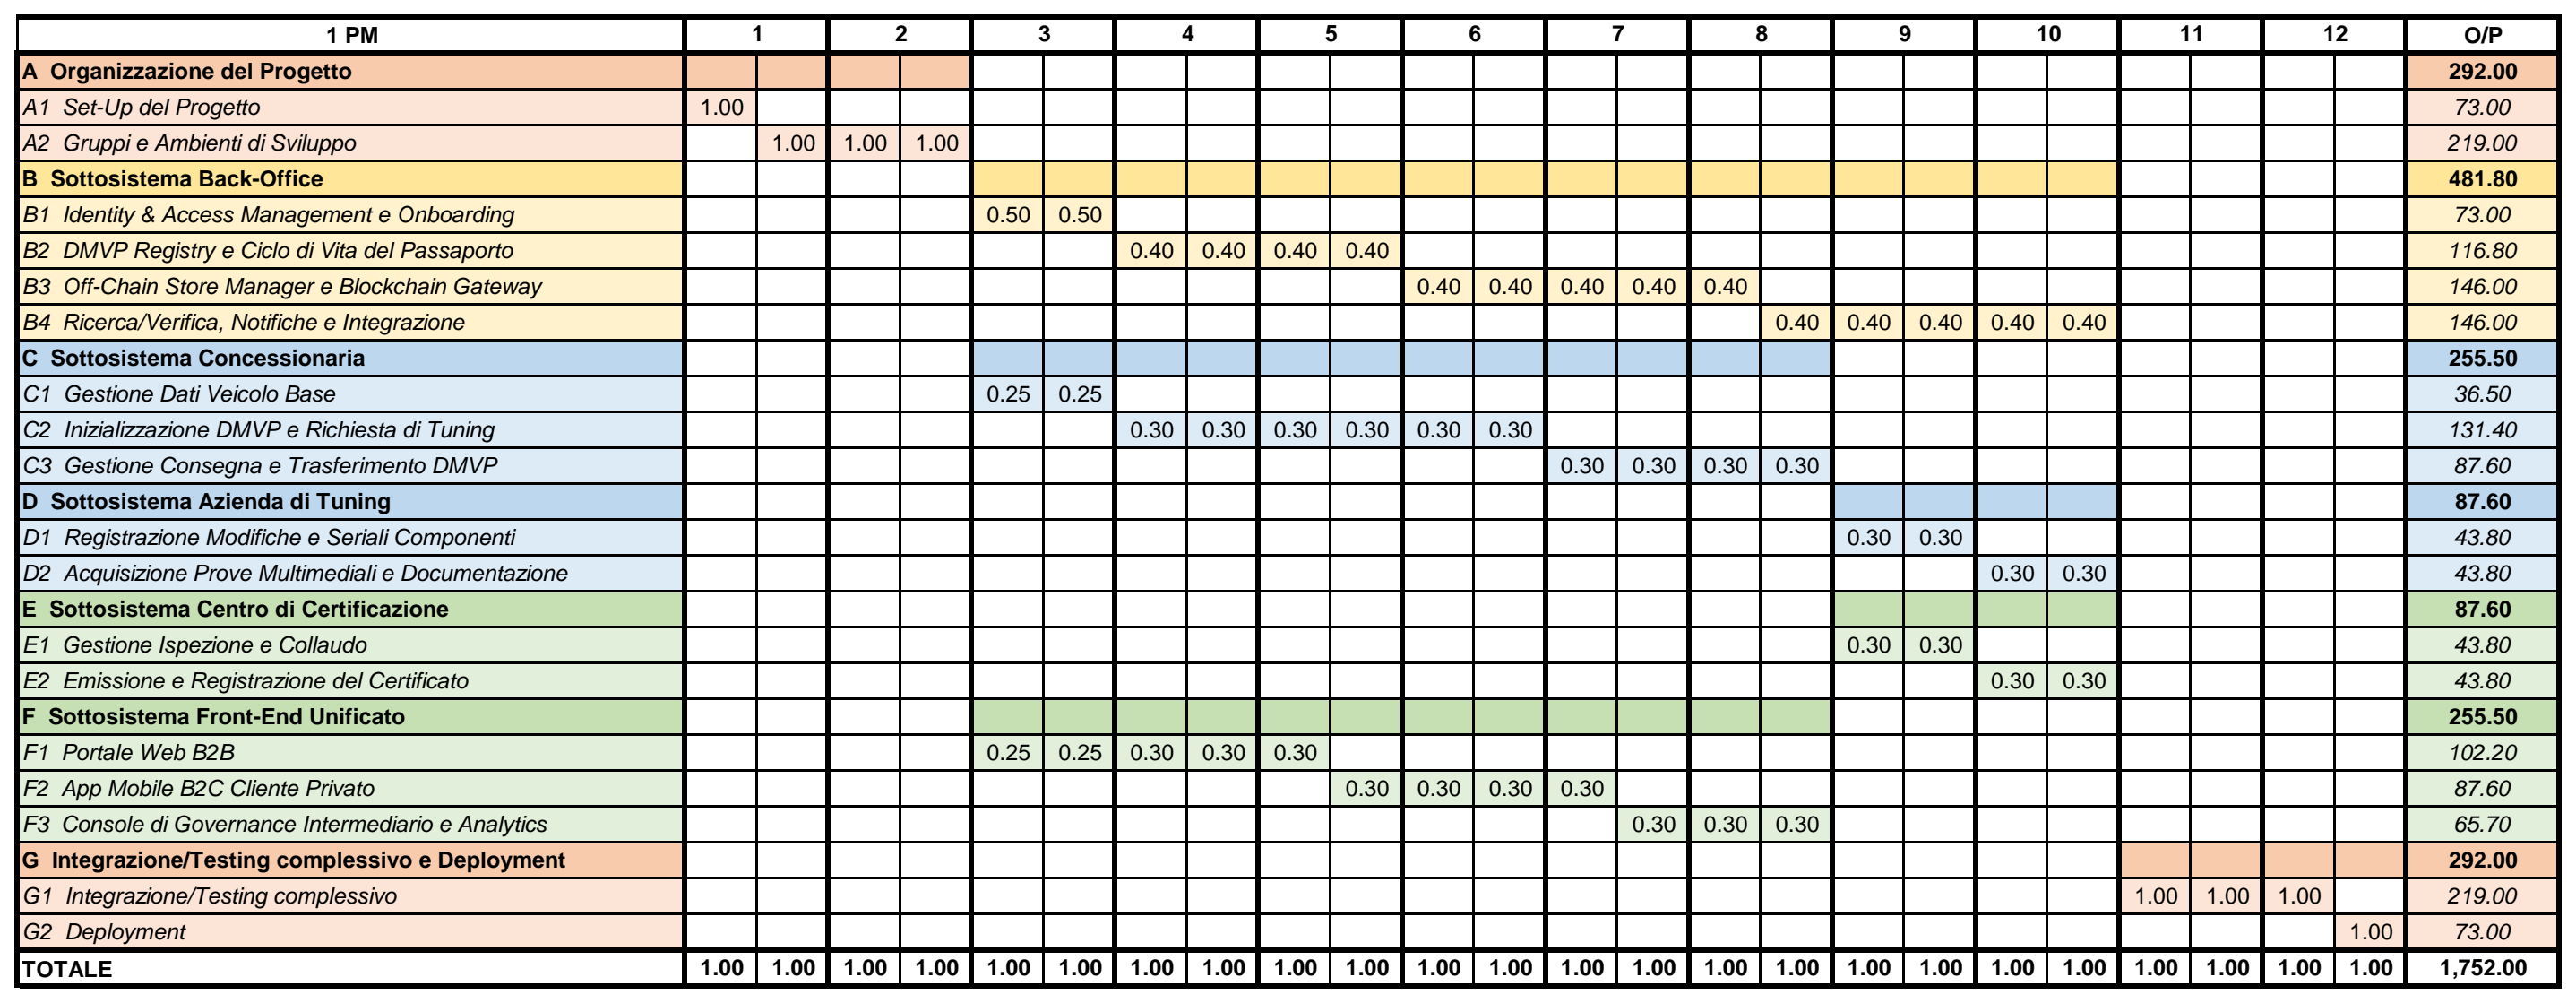
\includegraphics[width=\textwidth]{imgs/gantt/gantt_fase1/gantt_fase1_PM.png}
    \caption{Impegno del Project Manager nella Fase 1}
    \label{fig:impegno-pm-fase1}
\end{figure}
\begin{figure}[H]
    \centering
    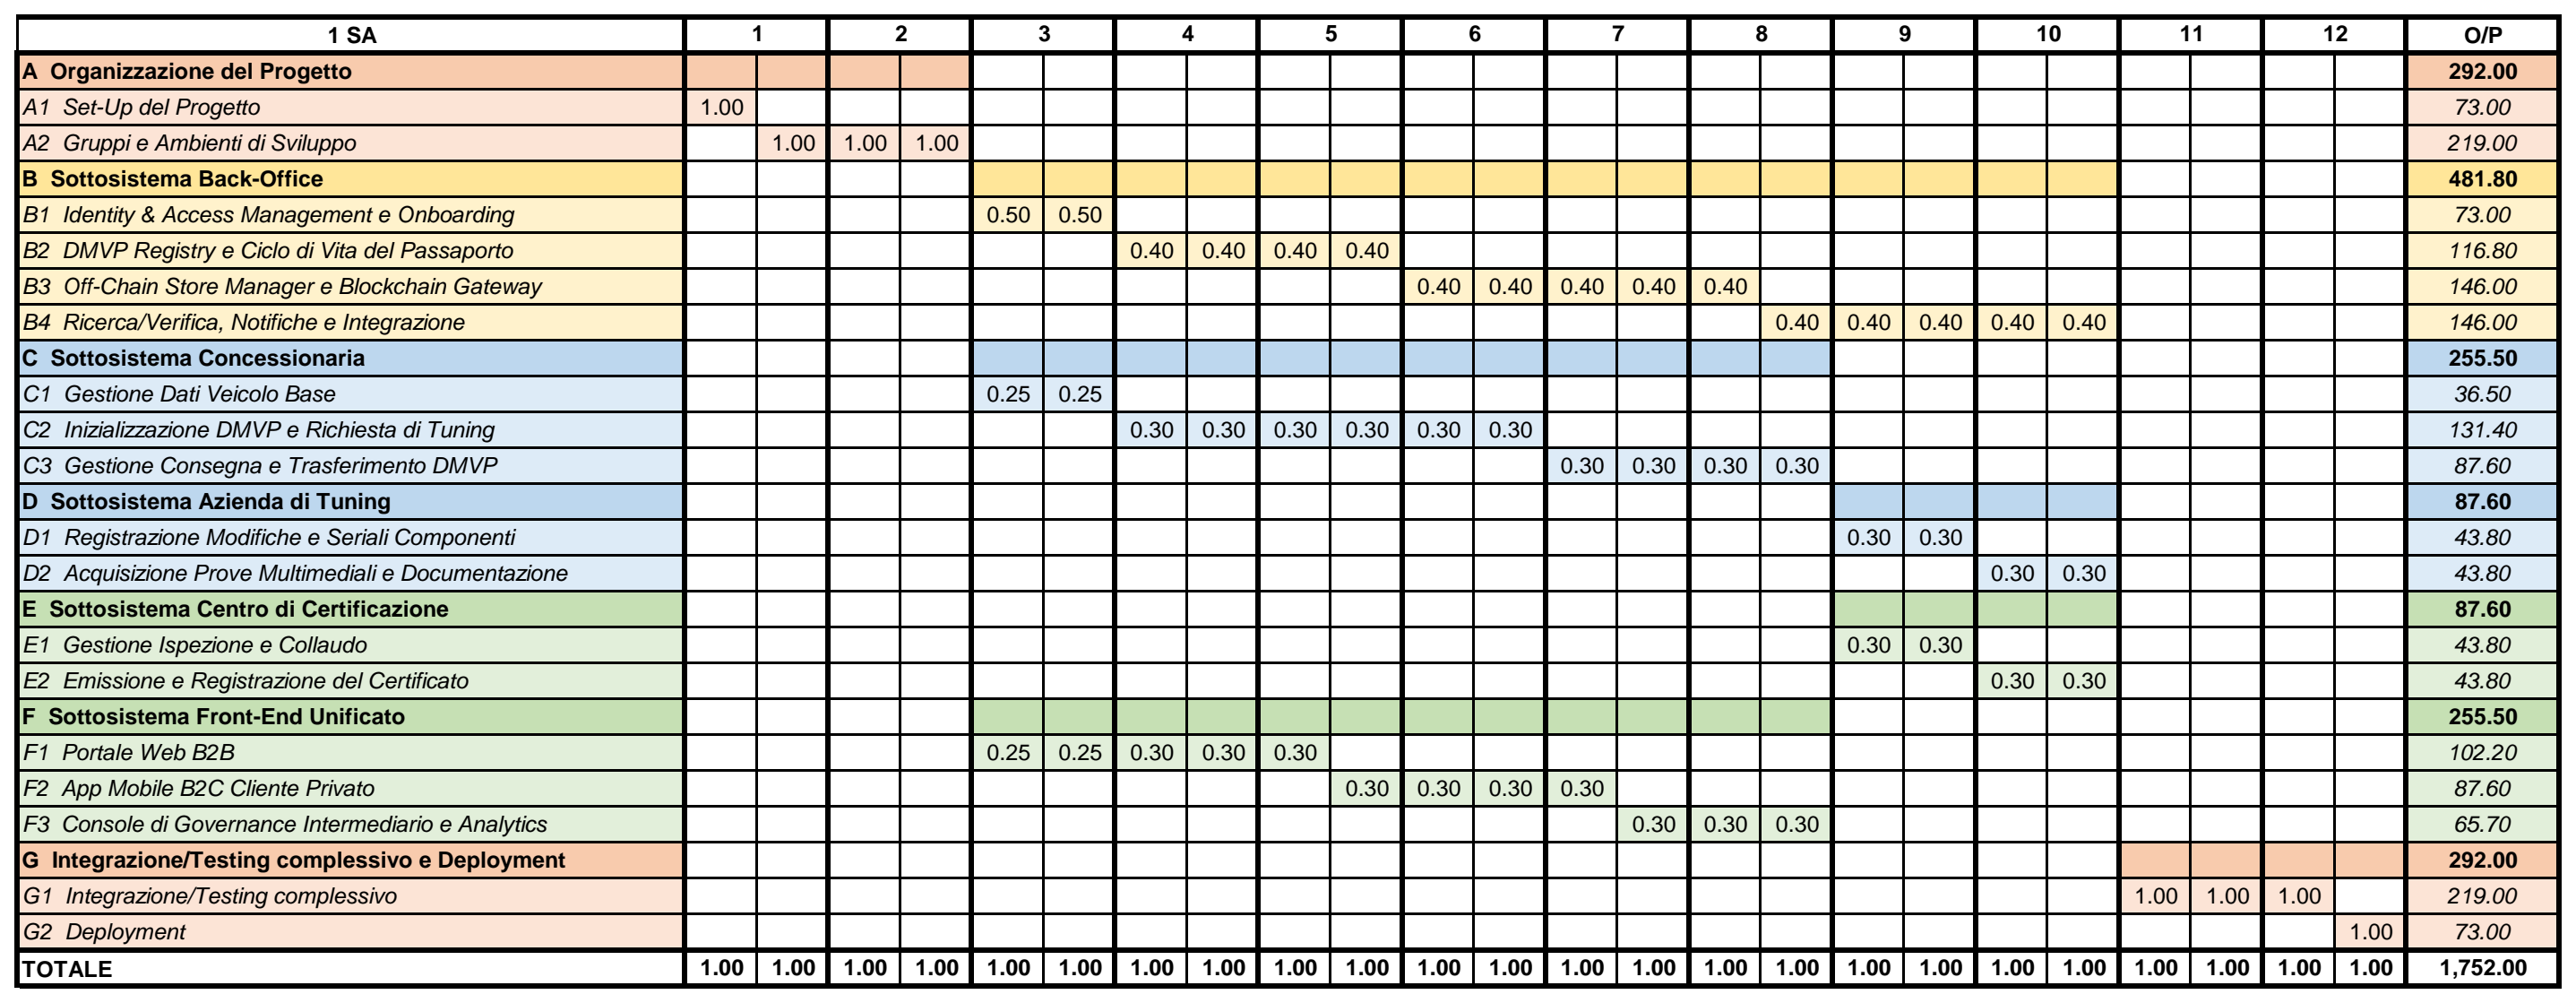
\includegraphics[width=\textwidth]{imgs/gantt/gantt_fase1/gantt_fase1_SA.png}
    \caption{Impegno del Software Architect nella Fase 1}
    \label{fig:impegno-sa-fase1}
\end{figure}
\begin{figure}[H]
    \centering
    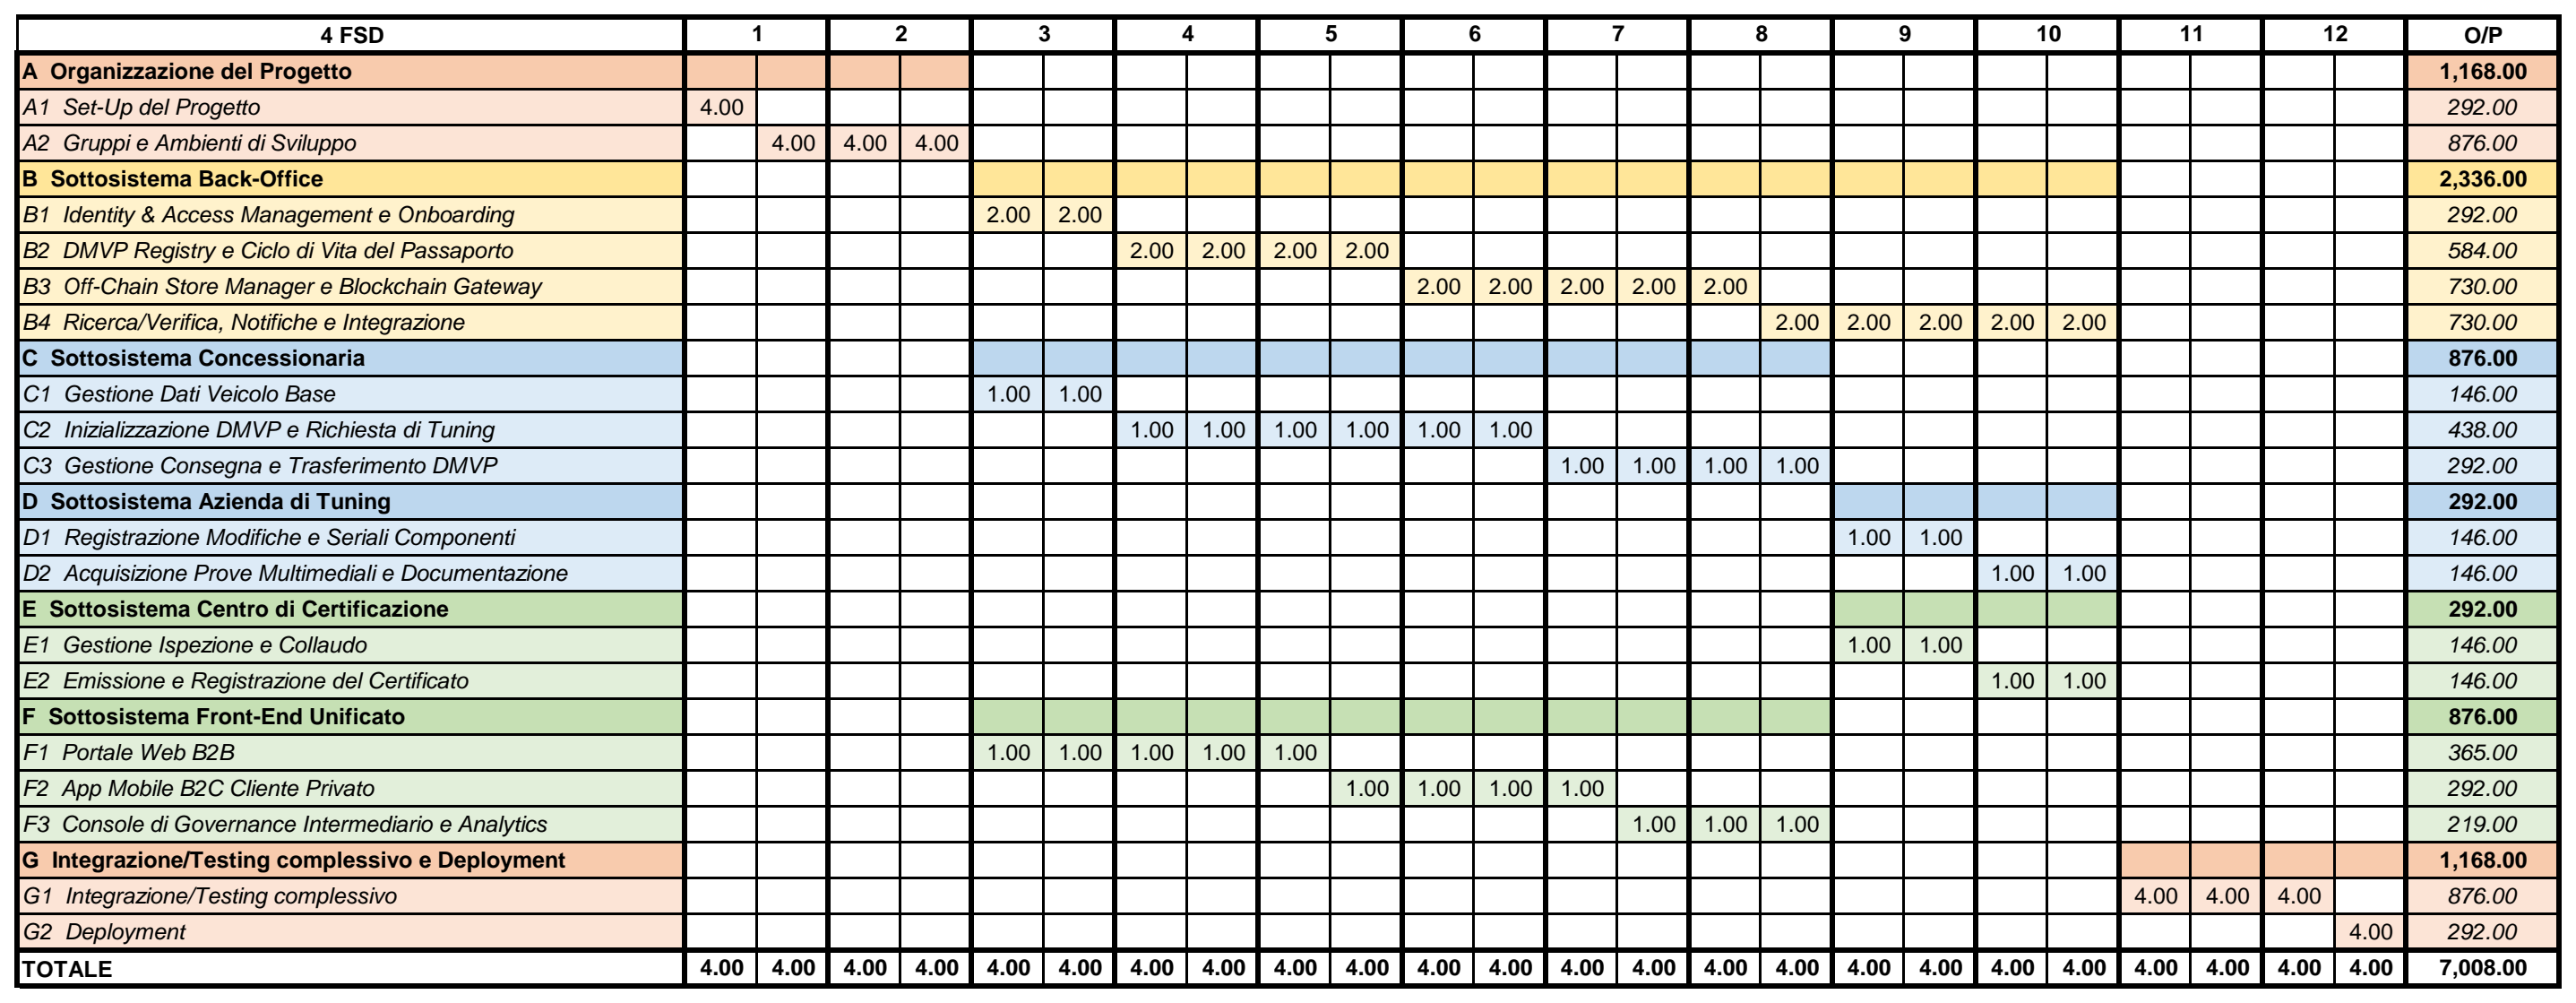
\includegraphics[width=\textwidth]{imgs/gantt/gantt_fase1/gantt_fase1_FSD.png}
    \caption{Impegno dei Full Stack Developer nella Fase 1}
    \label{fig:impegno-fsd-fase1}
\end{figure}
\begin{figure}[H]
    \centering
    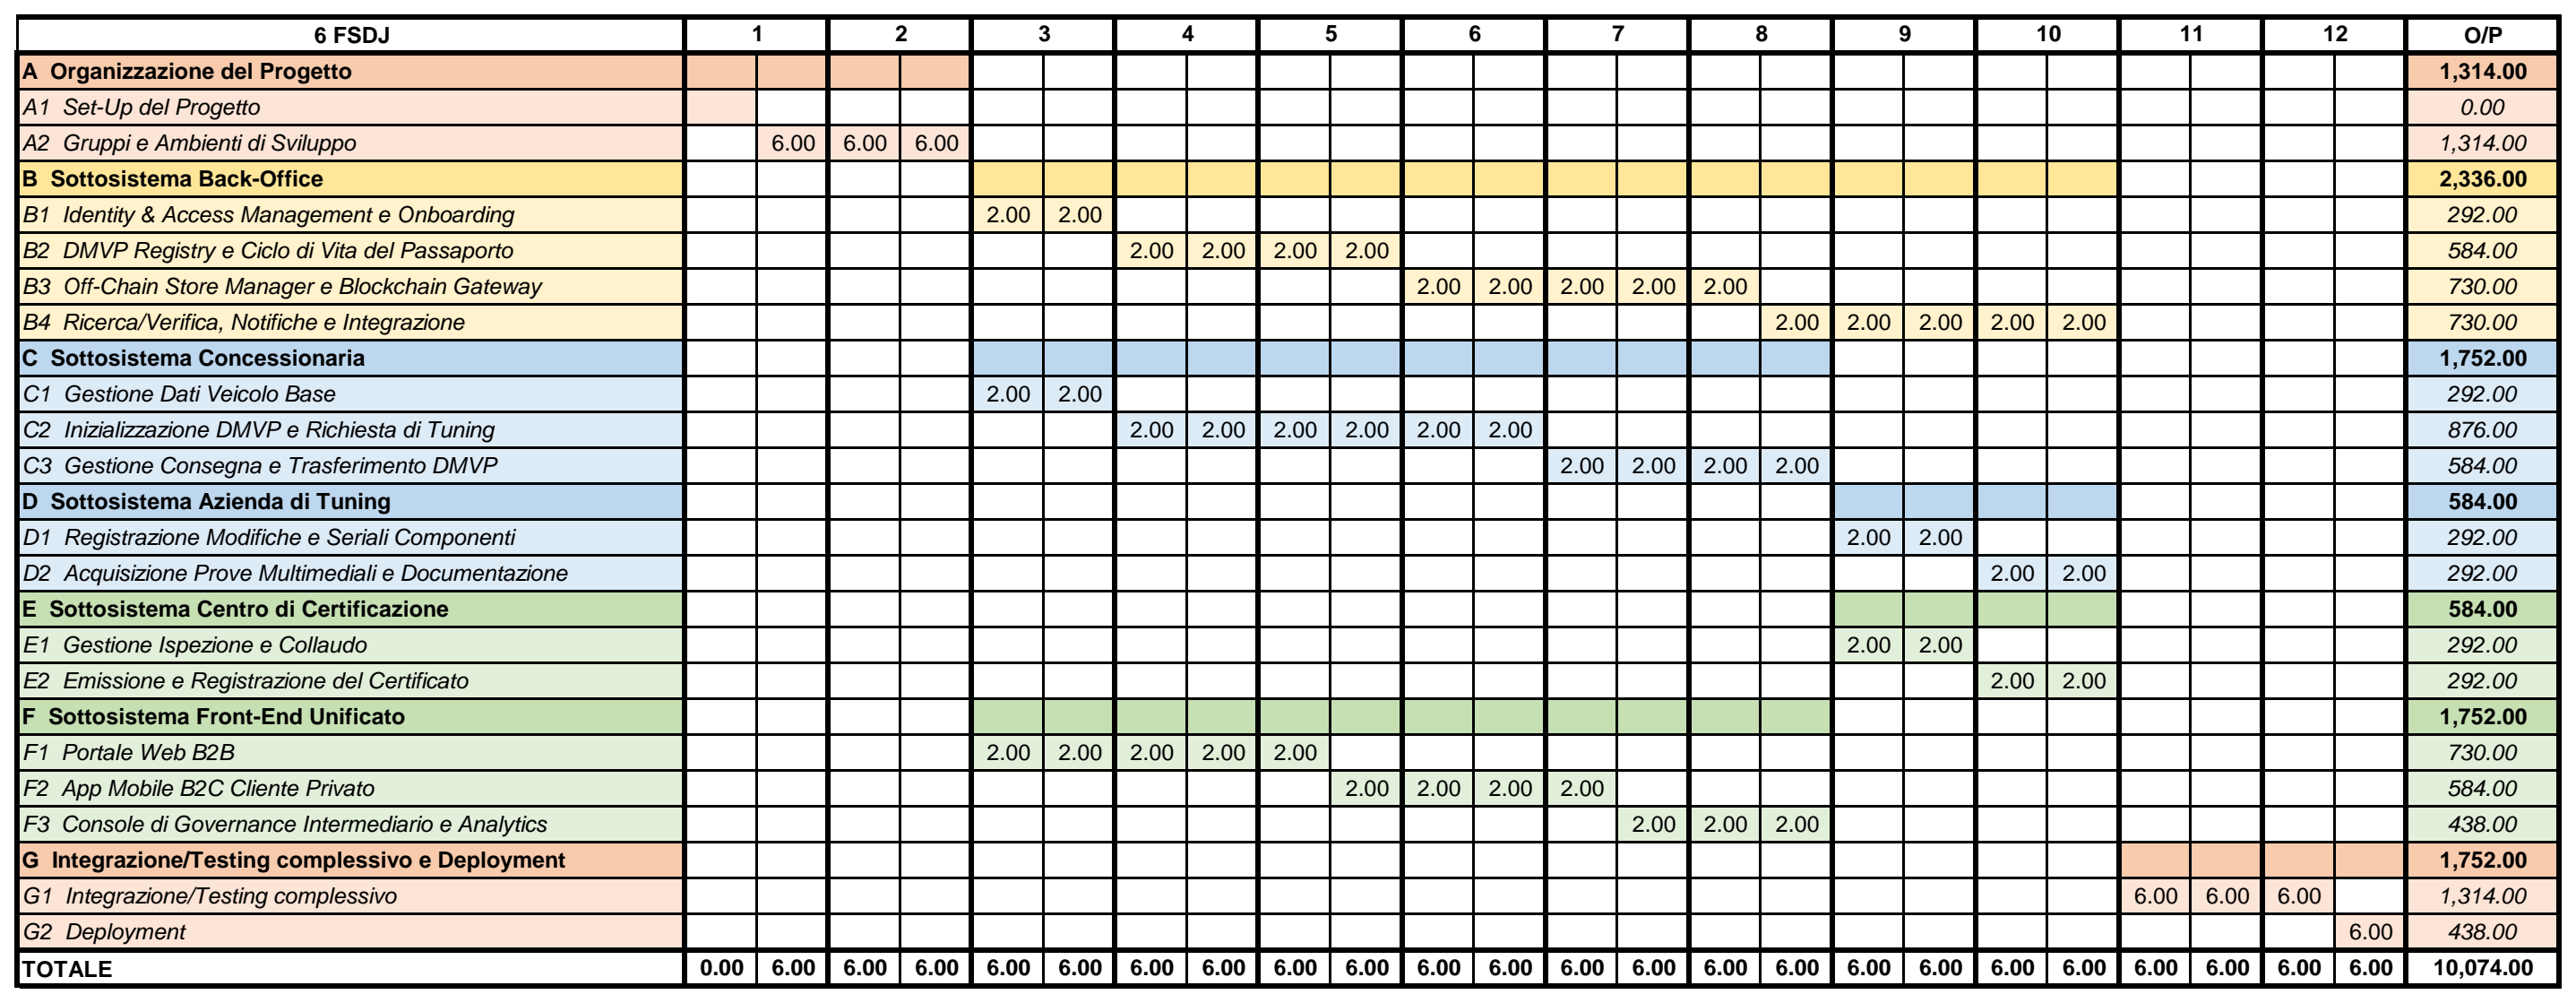
\includegraphics[width=\textwidth]{imgs/gantt/gantt_fase1/gantt_fase1_FSDJ.png}
    \caption{Impegno dei Full Stack Developer Junior nella Fase 1}
    \label{fig:impegno-fsdj-fase1}
\end{figure}
\begin{figure}[H]
    \centering
    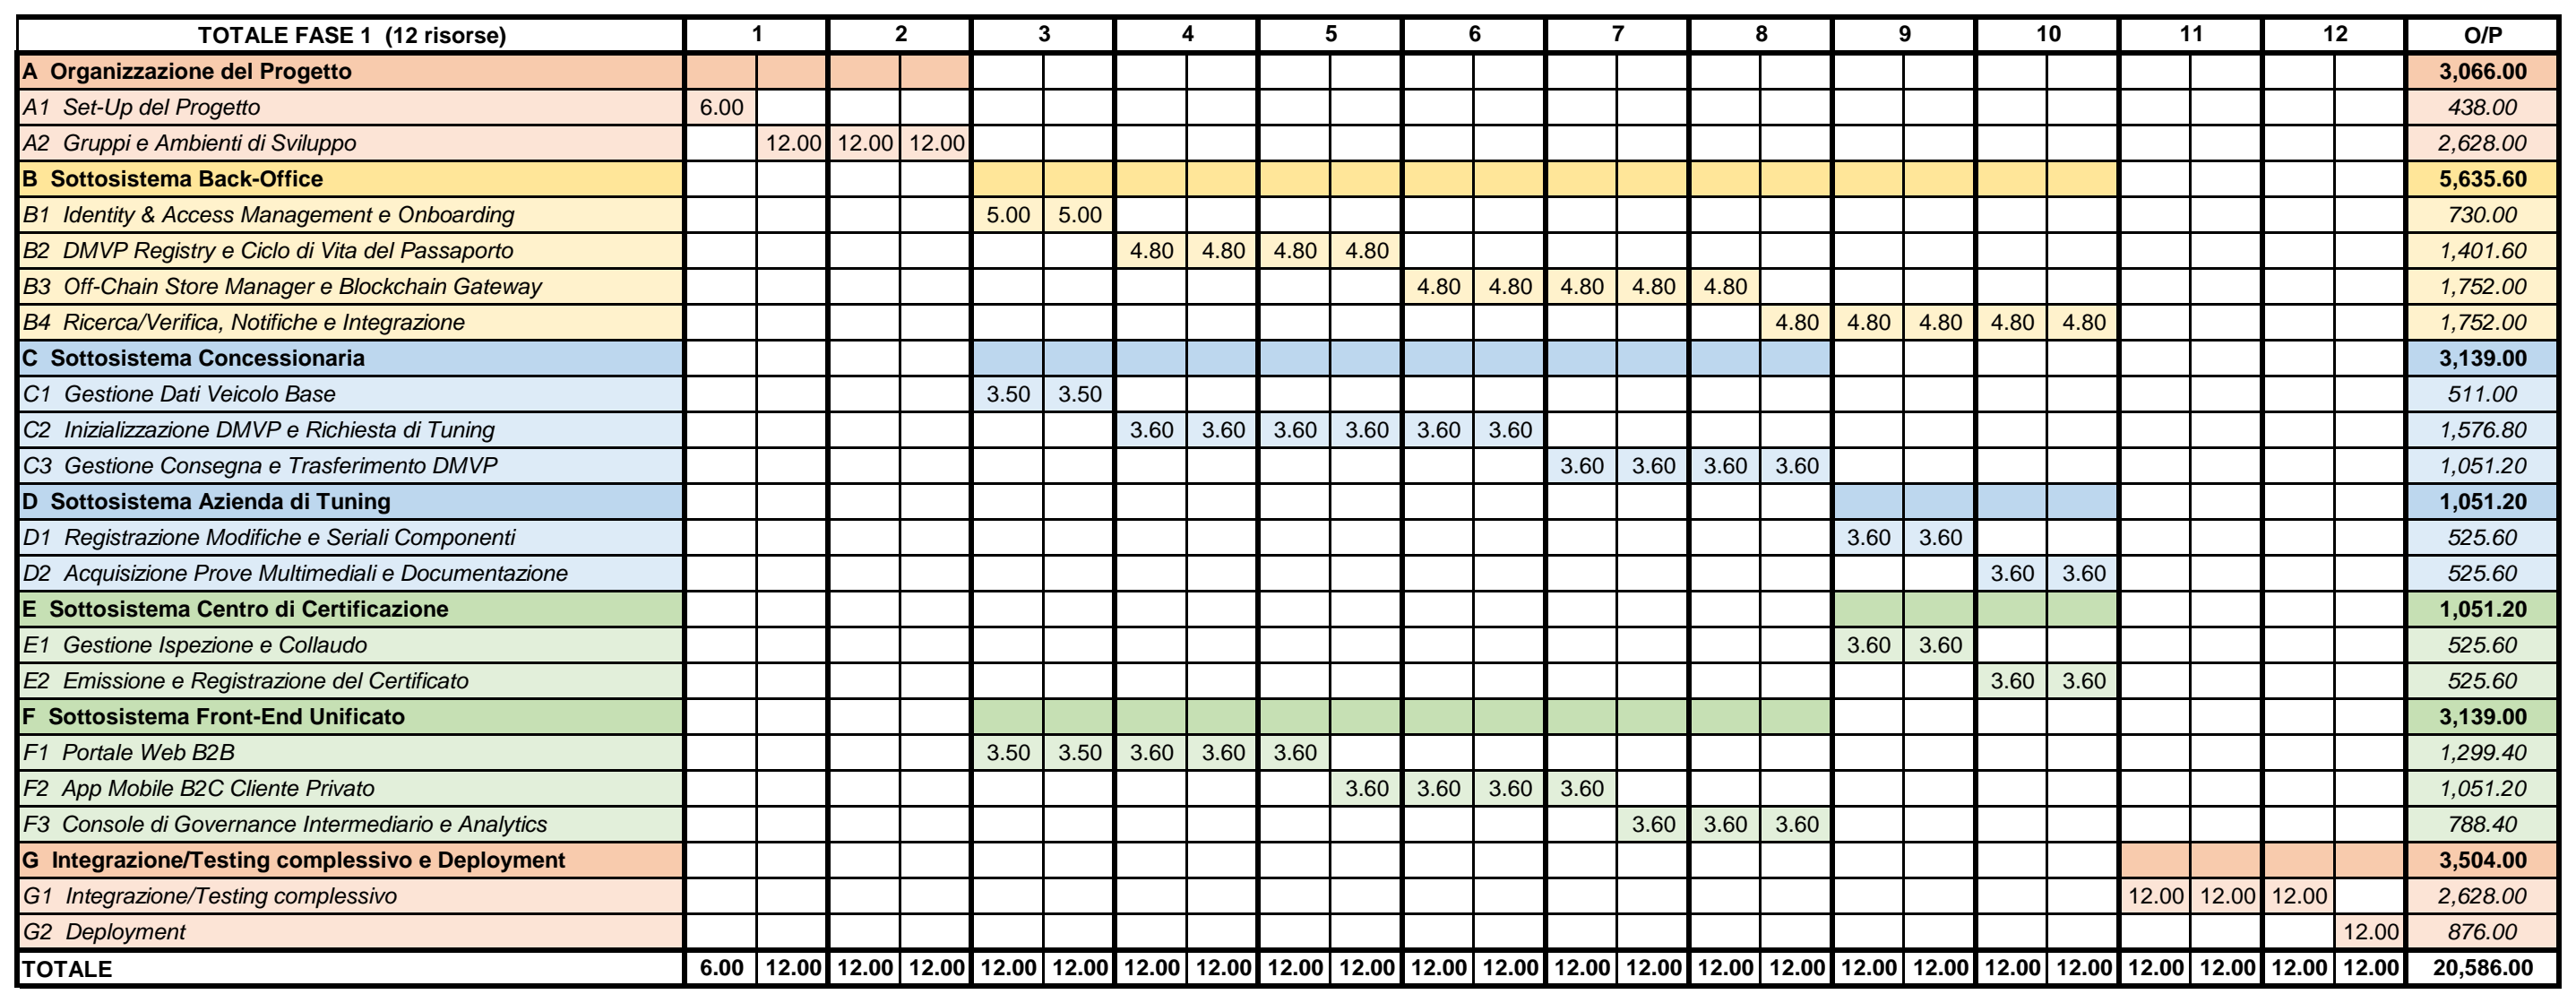
\includegraphics[width=\textwidth]{imgs/gantt/gantt_fase1/gantt_fase1_totale.png}
    \caption{Impegno totale delle risorse nella Fase 1}
    \label{fig:impegno-totale-fase1}
\end{figure}

\section{Pianificazione della Seconda Fase del Progetto: Esercizio della Piattaforma}

Successivamente alla pianificazione della prima fase, incentrata sullo sviluppo e sul rilascio della soluzione software, si rende necessaria la strutturazione della seconda fase del ciclo di vita del progetto, relativa al periodo di \textbf{esercizio, manutenzione e monitoraggio operativo} della piattaforma, su un orizzonte temporale di \textbf{cinque anni}.

Al fine di garantire la continuità operativa, l'integrità del registro distribuito e la progressiva espansione della rete, sono stati definiti cinque Task macro-funzionali, riassunti nella Tabella~\ref{tab:task-fase2}.

\begin{table}[H]
\centering
\small
\begin{tabular}{cp{4cm}p{7.5cm}}
\hline
\textbf{Cod.} & \textbf{Task} & \textbf{Descrizione} \\
\hline
A & Promozione della Piattaforma e Assistenza Commerciale & Campagne di marketing, presentazioni commerciali a concessionarie e reti di tuning, gestione delle trattative e personalizzazione dell'offerta. \\
B & Manutenzione Ordinaria & Aggiornamenti di sicurezza, correzione dei difetti, monitoraggio delle prestazioni e gestione dei nodi della rete permissioned. \\
C & Manutenzione Evolutiva & Nuove funzionalità in risposta alle esigenze degli utenti e alle evoluzioni normative; integrazione con nuovi sistemi esterni. \\
D & Assistenza e Onboarding degli Attori & Supporto tecnico e formazione di concessionarie, aziende di tuning e centri di certificazione; gestione delle identità di rete. \\
E & Analisi dei Dati di Esercizio & Raccolta e analisi dei dati d'uso, reportistica per gli attori business e supporto alle decisioni strategiche. \\
\hline
\end{tabular}
\caption{Task della Seconda Fase}
\label{tab:task-fase2}
\end{table}

La seconda fase non richiede l'impiego dell'intero organico iniziale, bensì prevede una contrazione strutturale del team per ottimizzare i costi di gestione. Il nucleo operativo viene ridotto da \textbf{12 a 8 risorse} complessive, riunite in un unico gruppo di gestione dell'esercizio (Figura~\ref{fig:gruppi-fase2}) così composto:

\begin{itemize}
    \item \textbf{0,5 Project Manager (PM)}, con funzioni di controllo di gestione e governance commerciale.
    \item \textbf{0,5 Software Architect (SA)}, incaricato della supervisione di alto livello dell'infrastruttura di rete.
    \item \textbf{2 Full Stack Developer (FSD)}, dedicati alla stabilità del back-end e dell'integrazione con la rete permissioned.
    \item \textbf{4 Full Stack Developer Junior (FSDJ)}, allocati sulle attività di assistenza e di aggiornamento delle interfacce.
\end{itemize}

\begin{figure}[H]
    \centering
    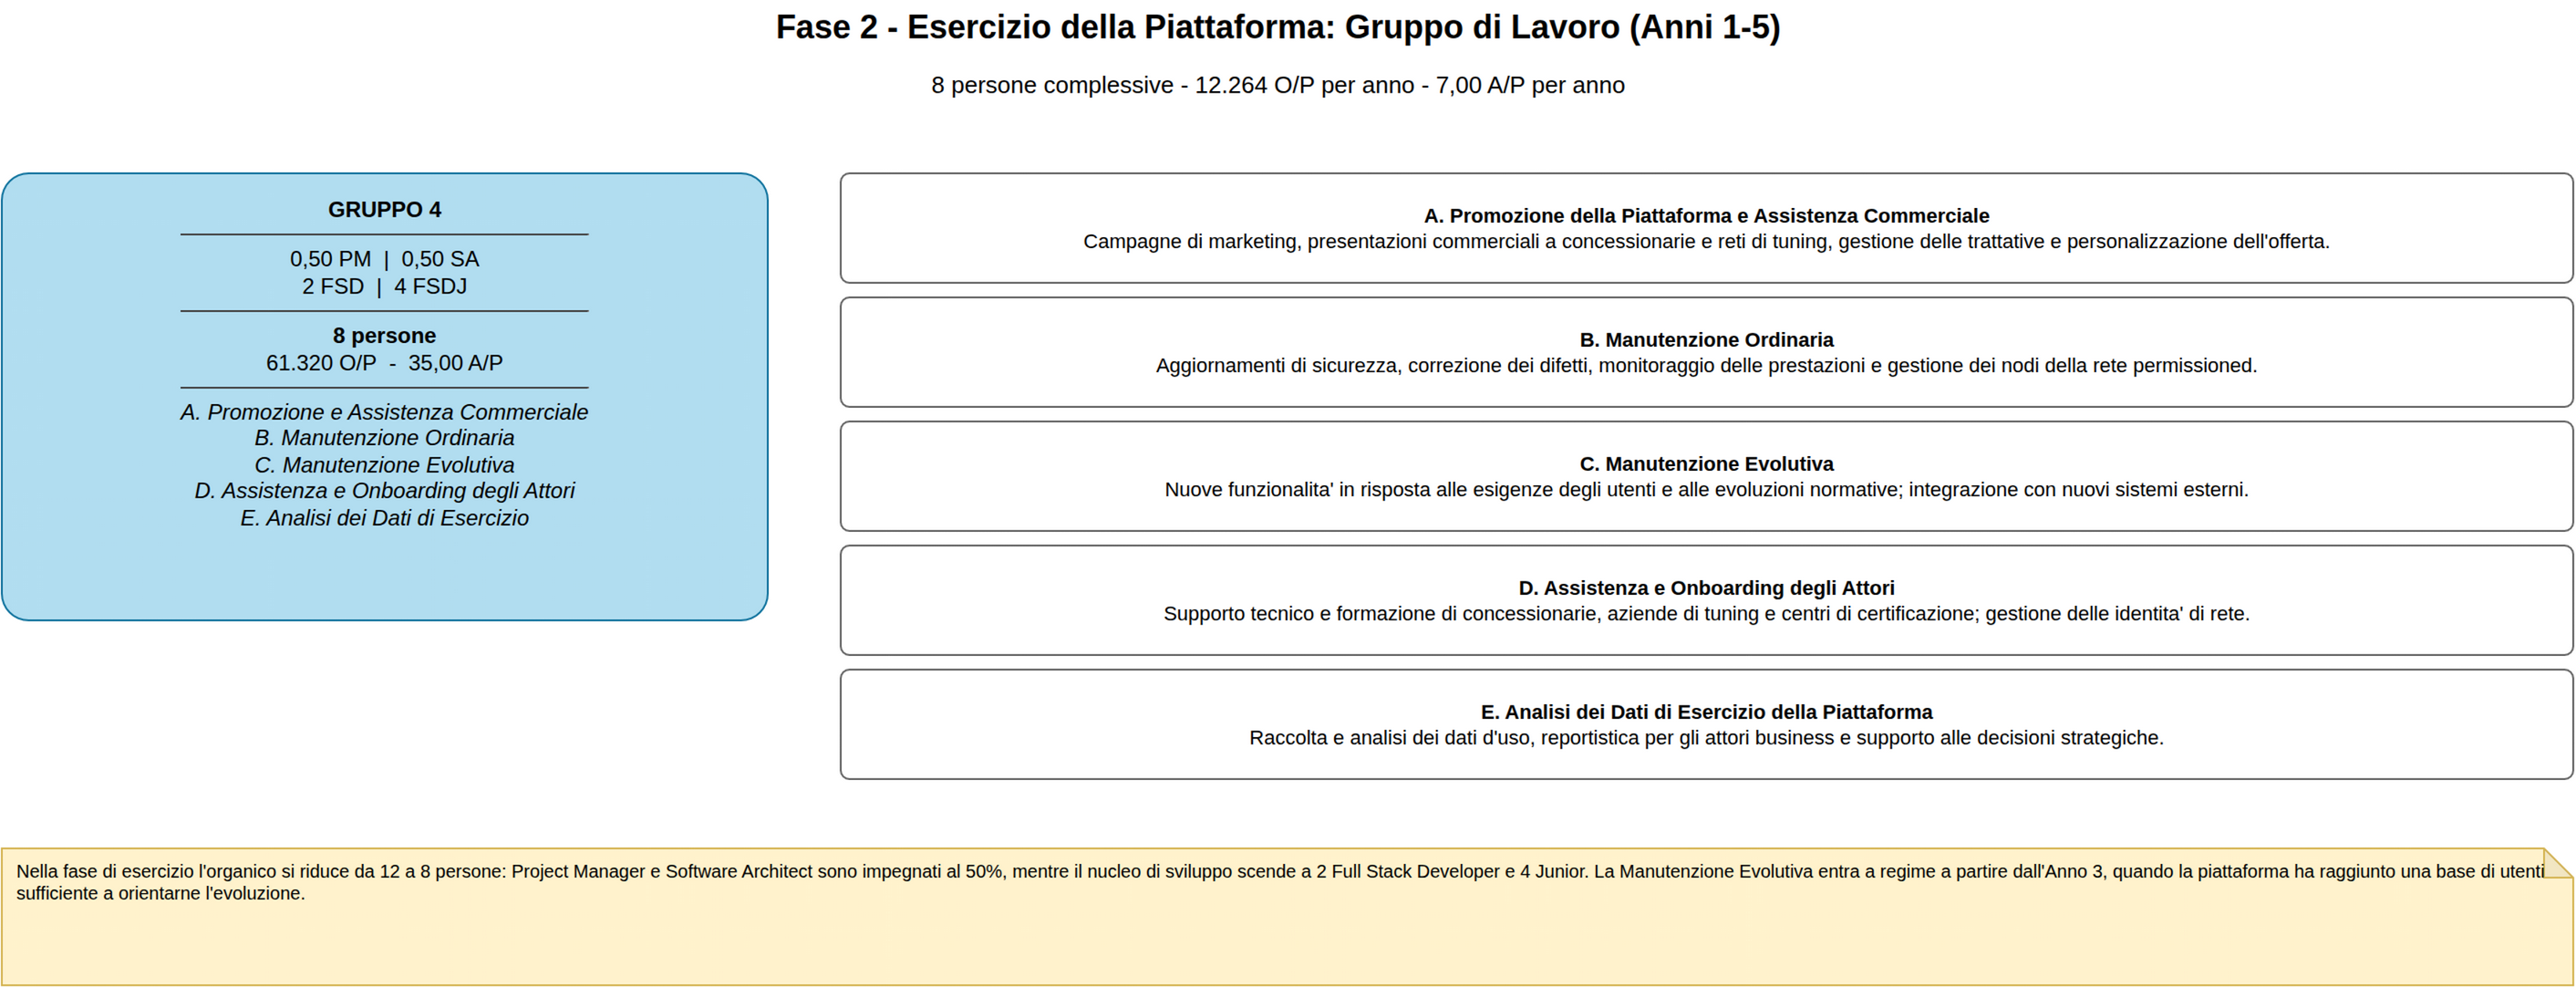
\includegraphics[width=\textwidth]{imgs/projectplan/09_gruppi_fase2.png}
    \caption{Gruppo di lavoro della Fase 2}
    \label{fig:gruppi-fase2}
\end{figure}

Il cronoprogramma delle attività per i cinque anni di esercizio prevede un impegno lineare e costante per l'\textbf{Analisi dei Dati di Esercizio}, che assorbe 1,55 A/P in ciascuno dei cinque anni, mentre gli altri task seguono un andamento articolato in due periodi distinti. Nei primi due anni le risorse si concentrano sulla \textbf{Manutenzione Ordinaria}, sull'\textbf{Assistenza e Onboarding degli Attori} e sulla \textbf{Promozione}, necessarie a stabilizzare la rete e ad acquisire i primi intermediari. A partire dall'\textbf{Anno 3} entra a regime la \textbf{Manutenzione Evolutiva}, quando la piattaforma ha raggiunto una base di utenti sufficiente a orientarne l'evoluzione: l'impegno su di essa (2,55 A/P) viene ricavato riducendo quello destinato agli altri tre task, la cui intensità si contrae una volta superata la fase di avviamento.

La ripartizione dell'impegno annuo tra i cinque Task \`e riportata nella Tabella~\ref{tab:op-fase2} e trova rappresentazione temporale nel diagramma di GANTT di Figura~\ref{fig:gantt-fase2}, articolato sui venti trimestri del quinquennio.

\begin{table}[H]
\centering
\small
\makebox[\textwidth][c]{%
\begin{tabular}{clrrrrrr}
\hline
\textbf{Cod.} & \textbf{Task} & \textbf{Anno 1} & \textbf{Anno 2} & \textbf{Anno 3} & \textbf{Anno 4} & \textbf{Anno 5} & \textbf{Totale} \\
\hline
A & Promozione e Assistenza Commerciale & 1.051,2 & 1.051,2 &   700,8 &   700,8 &   700,8 &  4.204,8 \\
B & Manutenzione Ordinaria                                & 5.080,8 & 5.080,8 & 2.277,6 & 2.277,6 & 2.277,6 & 16.994,4 \\
C & Manutenzione Evolutiva                                &       0 &       0 & 4.467,6 & 4.467,6 & 4.467,6 & 13.402,8 \\
D & Assistenza e Onboarding degli Attori                  & 3.416,4 & 3.416,4 & 2.102,4 & 2.102,4 & 2.102,4 & 13.140,0 \\
E & Analisi dei Dati di Esercizio & 2.715,6 & 2.715,6 & 2.715,6 & 2.715,6 & 2.715,6 & 13.578,0 \\
\hline
& \textbf{TOTALE O/P} & \textbf{12.264} & \textbf{12.264} & \textbf{12.264} & \textbf{12.264} & \textbf{12.264} & \textbf{61.320} \\
& \textbf{TOTALE A/P} & \textbf{7,00} & \textbf{7,00} & \textbf{7,00} & \textbf{7,00} & \textbf{7,00} & \textbf{35,00} \\
\hline
\end{tabular}}
\caption{Impegno annuo per Task della Seconda Fase (Ore-Persona)}
\label{tab:op-fase2}
\end{table}

\begin{figure}[H]
    \centering
    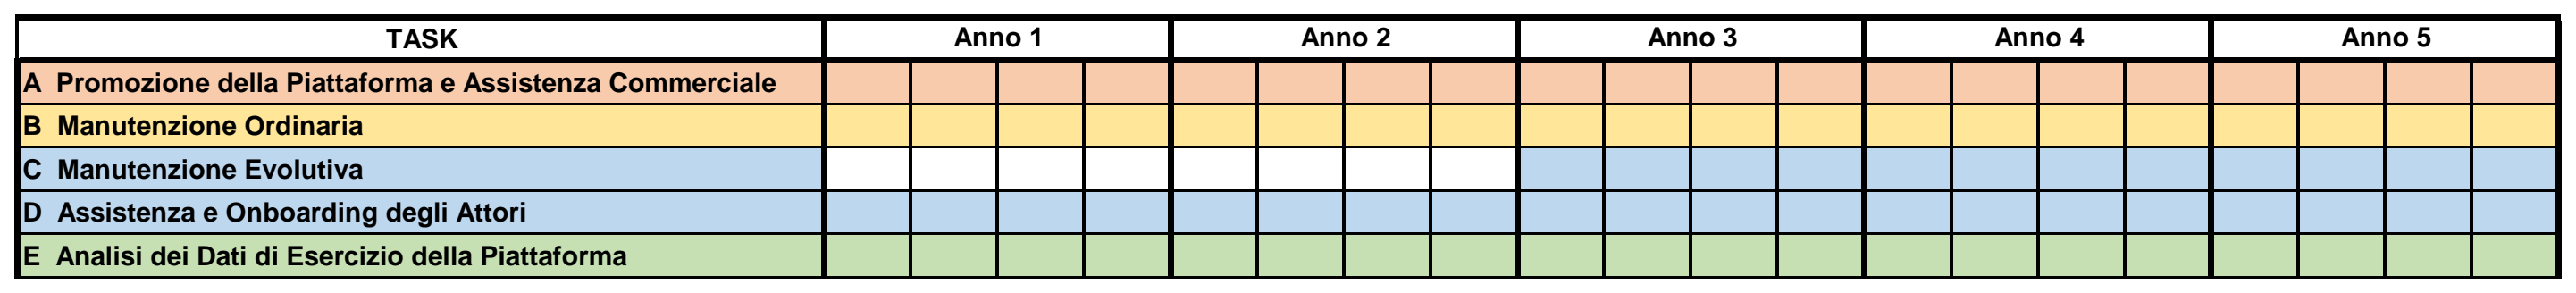
\includegraphics[width=\textwidth]{imgs/gantt/gantt_fase2/gantt_fase2.png}
    \caption{Diagramma di GANTT della Fase 2}
    \label{fig:gantt-fase2}
\end{figure}

L'impiego delle singole figure professionali nel corso del quinquennio di esercizio \`e riportato nei prospetti delle Figure~\ref{fig:impegno-pm-fase2}, \ref{fig:impegno-sa-fase2}, \ref{fig:impegno-fsd-fase2}, \ref{fig:impegno-fsdj-fase2} e~\ref{fig:impegno-totale-fase2}, costruiti con la medesima logica adottata per la Fase~1: l'unità temporale \`e in questo caso il trimestre, pari a 438 Ore-Persona per risorsa a tempo pieno, e il valore di ciascuna cella esprime il numero di risorse impegnate nel trimestre.

\begin{figure}[H]
    \centering
    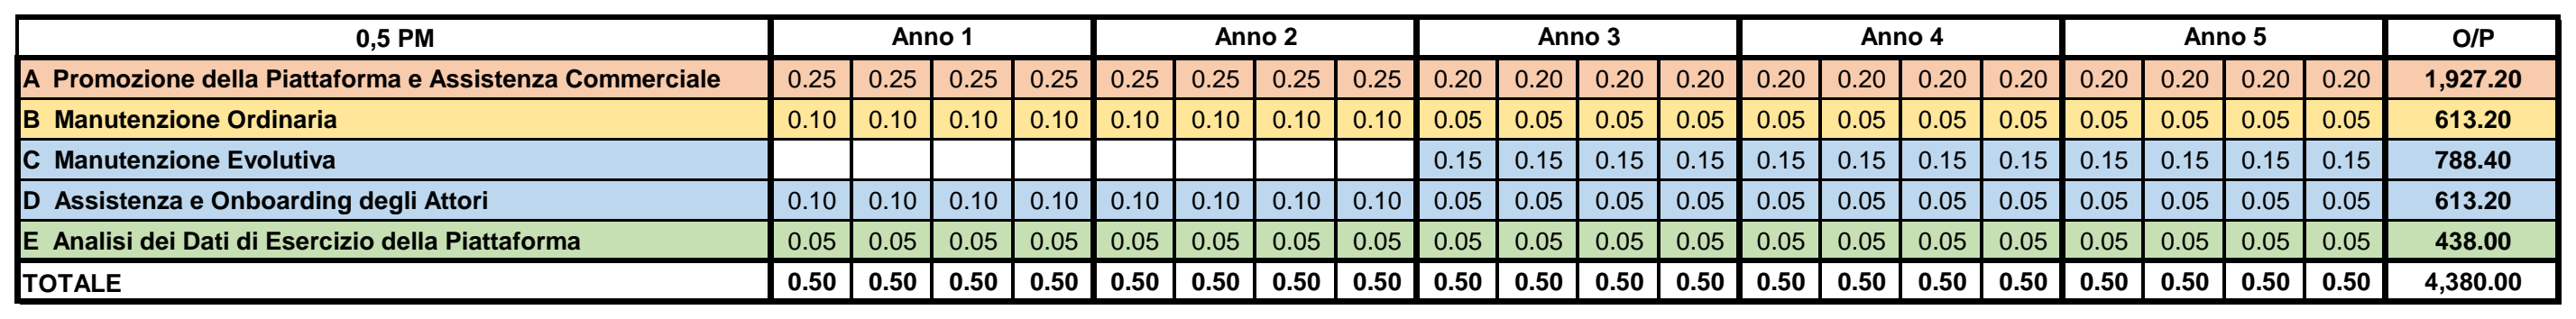
\includegraphics[width=\textwidth]{imgs/gantt/gantt_fase2/gantt_fase2_PM.png}
    \caption{Impegno del Project Manager nella Fase 2}
    \label{fig:impegno-pm-fase2}
\end{figure}
\begin{figure}[H]
    \centering
    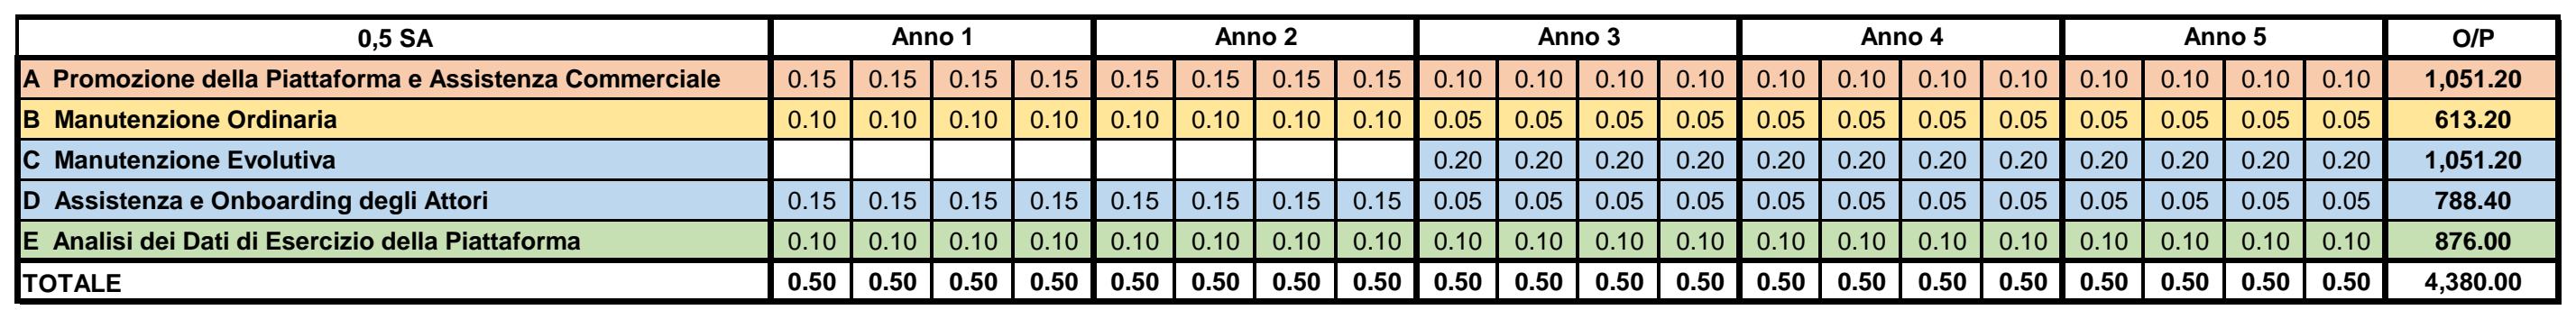
\includegraphics[width=\textwidth]{imgs/gantt/gantt_fase2/gantt_fase2_SA.png}
    \caption{Impegno del Software Architect nella Fase 2}
    \label{fig:impegno-sa-fase2}
\end{figure}
\begin{figure}[H]
    \centering
    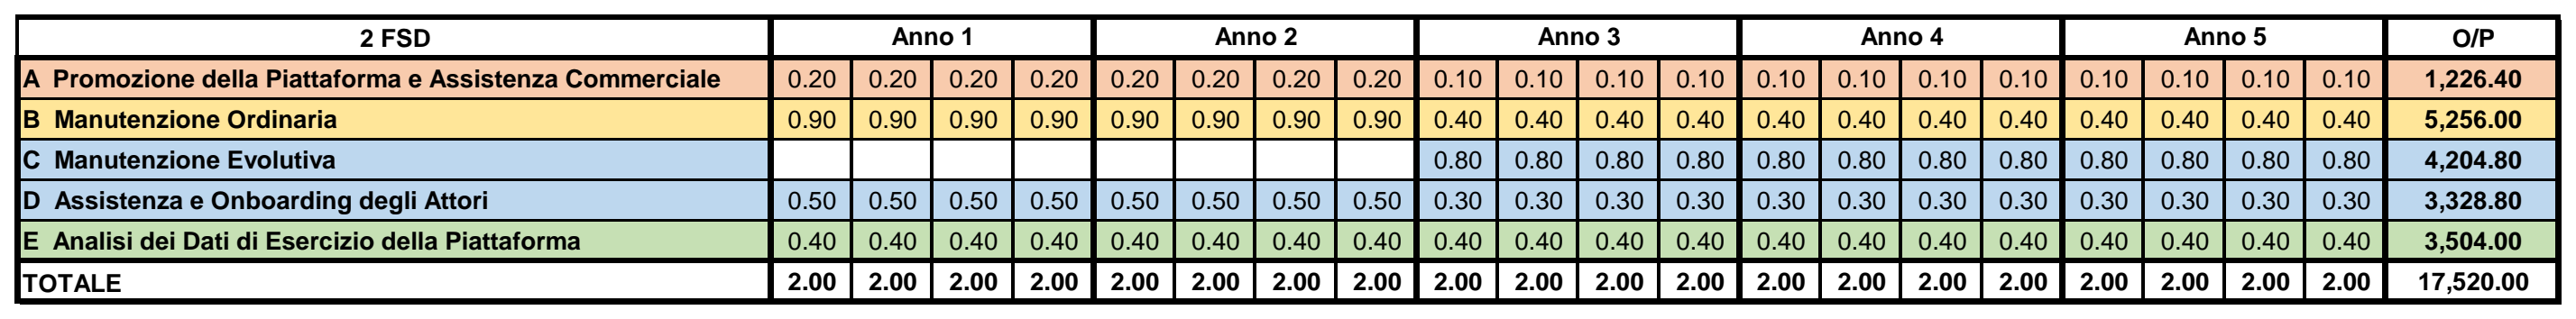
\includegraphics[width=\textwidth]{imgs/gantt/gantt_fase2/gantt_fase2_FSD.png}
    \caption{Impegno dei Full Stack Developer nella Fase 2}
    \label{fig:impegno-fsd-fase2}
\end{figure}
\begin{figure}[H]
    \centering
    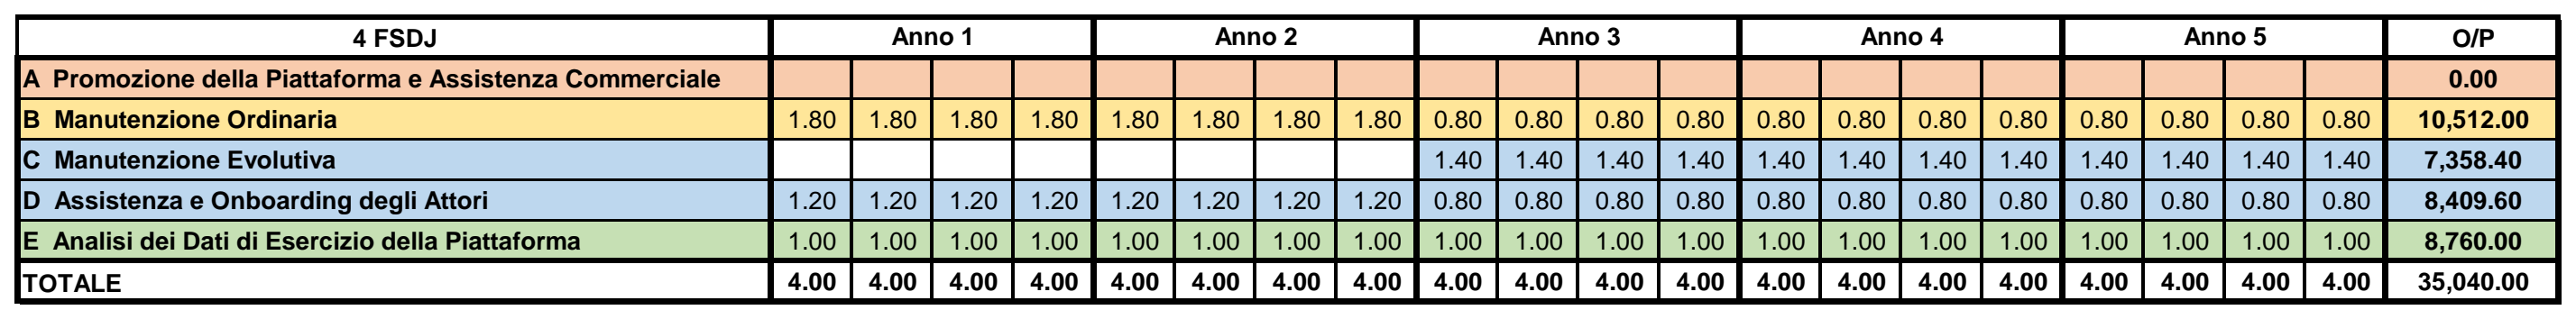
\includegraphics[width=\textwidth]{imgs/gantt/gantt_fase2/gantt_fase2_FSDJ.png}
    \caption{Impegno dei Full Stack Developer Junior nella Fase 2}
    \label{fig:impegno-fsdj-fase2}
\end{figure}
\begin{figure}[H]
    \centering
    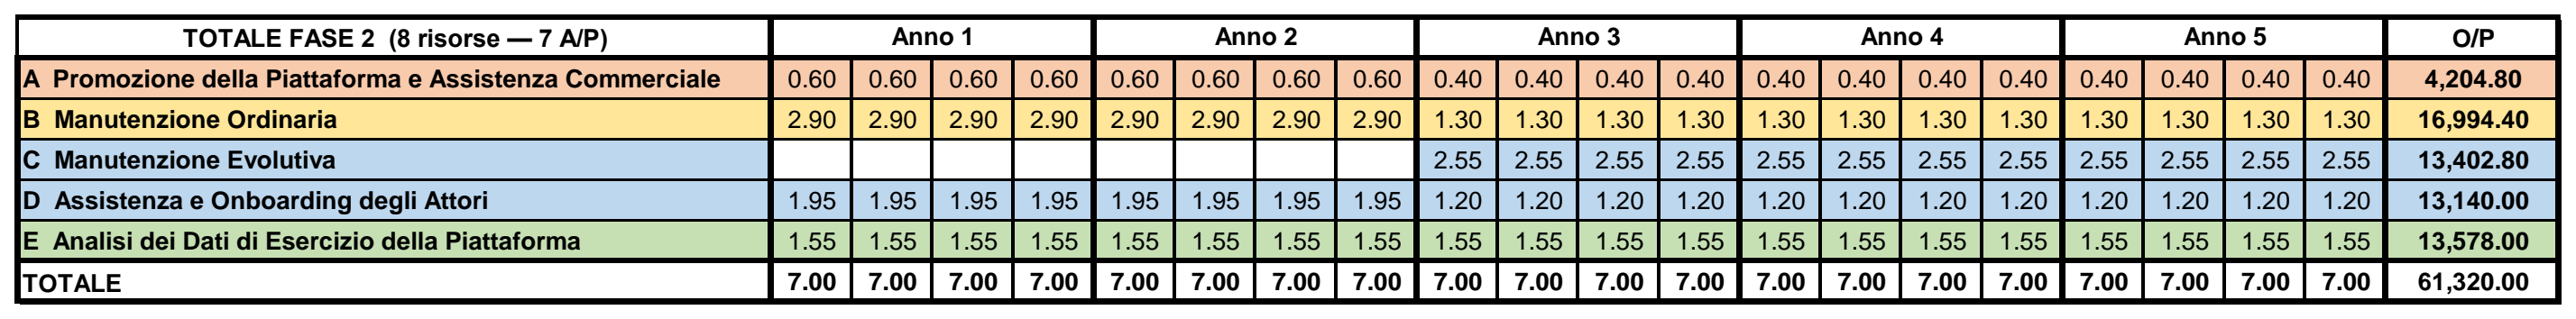
\includegraphics[width=\textwidth]{imgs/gantt/gantt_fase2/gantt_fase2_totale.png}
    \caption{Impegno totale delle risorse nella Fase 2}
    \label{fig:impegno-totale-fase2}
\end{figure}

\section{Riepilogo delle Risorse Umane Utilizzate}

A conclusione della pianificazione di progetto viene tracciato un quadro sinottico e comparativo dell'utilizzo delle risorse umane nel corso dei sei anni complessivi di ciclo di vita della piattaforma, evidenziando la transizione tra l'Anno 0 (Fase 1, sviluppo) e gli Anni 1--5 (Fase 2, esercizio).

L'impiego del personale, originariamente espresso in Ore-Persona (O/P), è riportato nella Tabella~\ref{tab:riepilogo-op} e successivamente convertito nell'unità di misura standard degli Anni-Persona (A/P) nella Tabella~\ref{tab:riepilogo-ap}, assumendo come parametro di riferimento un coefficiente di 1.752 ore lavorative annue per risorsa a tempo pieno.

\begin{table}[H]
\centering
\small
\makebox[\textwidth][c]{%
\begin{tabular}{lrrrrrrr}
\hline
\textbf{Figura} & \textbf{Anno 0} & \textbf{Anno 1} & \textbf{Anno 2} & \textbf{Anno 3} & \textbf{Anno 4} & \textbf{Anno 5} & \textbf{Totale} \\
\hline
PM   &  1.752 &    876 &    876 &    876 &    876 &    876 &  6.132 \\
SA   &  1.752 &    876 &    876 &    876 &    876 &    876 &  6.132 \\
FSD  &  7.008 &  3.504 &  3.504 &  3.504 &  3.504 &  3.504 & 24.528 \\
FSDJ & 10.074 &  7.008 &  7.008 &  7.008 &  7.008 &  7.008 & 45.114 \\
\hline
\textbf{TOTALE O/P} & \textbf{20.586} & \textbf{12.264} & \textbf{12.264} & \textbf{12.264} & \textbf{12.264} & \textbf{12.264} & \textbf{81.906} \\
\textbf{N.\ persone} & \textbf{12} & \textbf{8} & \textbf{8} & \textbf{8} & \textbf{8} & \textbf{8} & \\
\hline
\end{tabular}}
\caption{Impegno annuale del personale in Ore-Persona}
\label{tab:riepilogo-op}
\end{table}

\begin{table}[H]
\centering
\small
\makebox[\textwidth][c]{%
\begin{tabular}{lrrrrrrr}
\hline
\textbf{Figura} & \textbf{Anno 0} & \textbf{Anno 1} & \textbf{Anno 2} & \textbf{Anno 3} & \textbf{Anno 4} & \textbf{Anno 5} & \textbf{Totale} \\
\hline
PM   & 1,00 & 0,50 & 0,50 & 0,50 & 0,50 & 0,50 &  3,50 \\
SA   & 1,00 & 0,50 & 0,50 & 0,50 & 0,50 & 0,50 &  3,50 \\
FSD  & 4,00 & 2,00 & 2,00 & 2,00 & 2,00 & 2,00 & 14,00 \\
FSDJ & 5,75 & 4,00 & 4,00 & 4,00 & 4,00 & 4,00 & 25,75 \\
\hline
\textbf{TOTALE A/P} & \textbf{11,75} & \textbf{7,00} & \textbf{7,00} & \textbf{7,00} & \textbf{7,00} & \textbf{7,00} & \textbf{46,75} \\
\textbf{N.\ persone} & \textbf{12} & \textbf{8} & \textbf{8} & \textbf{8} & \textbf{8} & \textbf{8} & \\
\hline
\end{tabular}}
\caption{Impegno annuale del personale in Anni-Persona}
\label{tab:riepilogo-ap}
\end{table}

Come evidenziato dai dati, emerge una marcata differenziazione nel dimensionamento del personale in relazione alle specifiche sfide ingegneristiche di ciascun periodo:

\begin{enumerate}
    \item \textbf{Fase 1 (Sviluppo)}: richiede un team allargato e altamente specializzato, composto da \textbf{12 persone}. La forte concentrazione di sviluppatori (4 senior e 6 junior) si rende indispensabile per parallelizzare la costruzione dei cinque sottosistemi applicativi e della componente blockchain, minimizzando il \textit{Time-to-Market}.
    \item \textbf{Fase 2 (Esercizio)}: consente una contrazione del team a \textbf{8 persone}. Una volta effettuato il deployment e consolidato il chaincode sulla rete permissioned, le attività si spostano su compiti di monitoraggio, assistenza agli attori e rilascio di aggiornamenti incrementali, operazioni gestibili in piena sicurezza ed efficienza da un organico ridotto e ottimizzato.
\end{enumerate}

I valori di impegno riportati in questo capitolo costituiscono la base di calcolo per la stima dei costi del personale sviluppata nel Business Plan (Capitolo~7).
\chapter{Business Plan}

\section{Organizzazione Complessiva del Business Plan}

Il presente Business Plan ha l'obiettivo di valutare la sostenibilità economica e finanziaria di \textit{Tuning Ledger}, la piattaforma per la gestione del \textit{Digital Modified Vehicle Passport} (DMVP), il registro distribuito dedicato alla certificazione e alla tracciabilit\`a delle modifiche eseguite nel settore dell'automotive tuning.

Si assume che il progetto venga realizzato da una societ\`a di sviluppo software gi\`a operativa sul mercato, e non da una \textit{start-up}, impiegando esclusivamente personale interno. L'analisi finanziaria si sviluppa su un orizzonte temporale di \textbf{sei anni}, coerentemente con la pianificazione definita nel Project Plan (Capitolo~6):

\begin{itemize}
    \item \textbf{Fase 1 (Anno 0)}: progettazione, sviluppo e \textit{deployment} della piattaforma (durata 1 anno).
    \item \textbf{Fase 2 (Anni 1-5)}: promozione, commercializzazione, erogazione dei servizi di assistenza e manutenzione evolutiva (durata 5 anni).
\end{itemize}

Per la stima dei costi del personale si assume la quota standard di \textbf{1.752 ore lavorative} per un Anno/Persona (A/P), equivalenti a 219 giornate lavorative da 8 ore. Di seguito vengono analizzate le componenti di costo impiegate in entrambe le fasi.

\subsection{Costi del Personale}

Le figure professionali coinvolte nel progetto sono quelle individuate nel Project Plan. Per ciascun profilo viene esplicitata la classificazione contrattuale in conformit\`a con i livelli stabiliti dal Contratto Collettivo Nazionale dei Metalmeccanici attualmente in vigore:

\begin{itemize}
    \item \textbf{Project Manager (PM)}: livello Quadro (ex 8\textdegree{} livello), con retribuzione lorda mensile di 2.493,21 \euro{} e superminimo di 1.000,00 \euro{}.
    \item \textbf{Software Architect (SA)}: livello B3 (ex 7\textdegree{} livello), con retribuzione lorda mensile di 2.336,00 \euro{} e superminimo di 500,00 \euro{}.
    \item \textbf{Full Stack Developer (FSD)}: livello B2 (ex 6\textdegree{} livello), con retribuzione lorda mensile di 2.092,45 \euro{} e superminimo di 200,00 \euro{}.
    \item \textbf{Full Stack Developer Junior (FSDJ)}: livello B1 (ex 5\textdegree{} Super), con retribuzione lorda mensile di 1.950,39 \euro{}, senza superminimo.
\end{itemize}

La Retribuzione Annua Lorda (RAL) si ottiene moltiplicando la retribuzione mensile globale, comprensiva di eventuale superminimo, per tredici mensilit\`a. Al fine di determinare il costo aziendale effettivo, alla RAL sono stati addizionati i seguenti elementi, con gli esiti riepilogati in Tabella~\ref{tab:costo-personale}:

\begin{itemize}
    \item \textbf{Trattamento di Fine Rapporto (TFR)}: calcolato mediante la formula RAL / 13,5, equivalente a poco meno di una mensilit\`a aggiuntiva.
    \item \textbf{Oneri previdenziali a carico dell'azienda}: determinati sulla base di un'aliquota contributiva complessiva stimata al 36\% della RAL, ripartita in due terzi a carico del datore di lavoro (\textbf{24\%}) e un terzo a carico del lavoratore (12\%).
\end{itemize}

\begin{table}[H]
\centering
\begin{tabular}{lrrrr}
\hline
\textbf{Profilo} & \textbf{RAL} & \textbf{TFR} & \textbf{Oneri azienda} & \textbf{Costo annuo} \\
\hline
PM   & 45.411,73 & 3.363,83 & 10.898,82 & 59.674,38 \\
SA   & 36.868,00 & 2.730,96 &  8.848,32 & 48.447,28 \\
FSD  & 29.801,85 & 2.207,54 &  7.152,44 & 39.161,84 \\
FSDJ & 25.355,07 & 1.878,15 &  6.085,22 & 33.318,44 \\
\hline
\end{tabular}
\caption{Costo lordo aziendale annuo per figura professionale (valori in \euro)}
\label{tab:costo-personale}
\end{table}

\subsection{Spese Generali}

Nell'assetto economico aziendale, le spese generali raggruppano tutti gli oneri necessari a garantire la continuit\`a e il corretto funzionamento delle attivit\`a operative, incluse le fasi di sviluppo software. Pur non essendo direttamente imputabili alla realizzazione del singolo servizio, tali costi risultano essenziali per il supporto dell'intera struttura d'impresa. Tra le principali voci si distinguono:

\begin{itemize}
    \item \textbf{Affitti e locazioni}: canoni relativi agli spazi aziendali destinati a uffici e aree operative.
    \item \textbf{Spese amministrative e gestionali}: costi legati sia al personale interno deputato al management, sia a servizi professionali esterni quali lo studio commercialista per la contabilit\`a e il consulente del lavoro per l'elaborazione dei cedolini.
    \item \textbf{Utenze e servizi infrastrutturali}: oneri per energia elettrica, riscaldamento, connettivit\`a e servizi di base necessari al mantenimento dell'infrastruttura aziendale.
\end{itemize}

Al fine di semplificare la valutazione dell'incidenza di tali flussi di spesa sul budget complessivo, l'analisi adotta una stima forfettaria pari al \textbf{20\% del costo totale del personale}.

\subsection{Costi per il Cloud Computing}

Nel contesto di un'azienda di sviluppo software, i costi legati alle risorse di calcolo e di memorizzazione non rientrano tra le spese generali, in quanto direttamente imputabili alle attivit\`a tecnico-operative. L'adozione di soluzioni \textit{cloud} consente di ottimizzare l'efficienza finanziaria tramite modelli di \textit{pricing} basati sul consumo effettivo (\textit{pay-per-use}), azzerando gli investimenti iniziali in hardware e i relativi costi di manutenzione.

Si assume pertanto che i servizi computazionali e di storage siano erogati interamente in cloud, ivi compresi i nodi della rete \textit{permissioned} e il database \textit{off-chain} destinato alla documentazione tecnica associata al DMVP. Il costo associato a ciascuna unit\`a $X$ del gruppo di lavoro \`e determinato mediante la seguente equazione:

\begin{equation}
    \text{Costo Totale} = (C_M \times 12) + (C_O \times N_O)
\end{equation}

dove $C_M$ \`e il costo fisso mensile del servizio cloud, $C_O$ il costo orario delle risorse di calcolo e $N_O$ il numero annuo di ore di utilizzo previsto per ciascun ruolo. Per la simulazione d'impatto sono stati adottati i valori $C_M = 20$ \euro{} e $C_O = 2$ \euro{}, con il seguente monte ore annuo: 600 ore per il Project Manager, 1.100 ore per il Software Architect e 1.300 ore per ciascun Full Stack Developer, senior e junior. Ne derivano i costi annui per persona riportati in Tabella~\ref{tab:cloud}.

\begin{table}[H]
\centering
\begin{tabular}{lrr}
\hline
\textbf{Profilo} & \textbf{Ore annue} & \textbf{Costo annuo} \\
\hline
PM   &   600 & 1.440,00 \\
SA   & 1.100 & 2.440,00 \\
FSD  & 1.300 & 2.840,00 \\
FSDJ & 1.300 & 2.840,00 \\
\hline
\end{tabular}
\caption{Costo annuo del cloud computing per unit\`a di personale (valori in \euro)}
\label{tab:cloud}
\end{table}

\subsection{Costi per Oneri Finanziari e Tassazione}

Gli oneri finanziari rappresentano i costi derivanti dagli interessi passivi sui capitali di terzi, necessari a coprire il fabbisogno di liquidit\`a del progetto nelle fasi antecedenti la generazione dei flussi di ricavo attesi. L'accesso alle linee di credito non costituisce tuttavia un processo automatico: gli istituti di credito subordinano l'erogazione dei finanziamenti a una rigorosa valutazione del merito creditizio dell'azienda, richiedendo idonee garanzie patrimoniali e un'approfondita analisi della sostenibilit\`a economico-finanziaria dell'iniziativa. Per la pianificazione del presente progetto, l'incidenza degli oneri finanziari \`e stata stimata prudenzialmente applicando un tasso d'interesse pari al \textbf{12\% annuo} sull'ammontare del capitale finanziato.

Oltre agli interessi passivi, la pianificazione finanziaria deve integrare la componente fiscale, rappresentata dall'Imposta sul Reddito delle Societ\`a (\textbf{IRES}, con aliquota del 24\%) e dall'Imposta Regionale sulle Attivit\`a Produttive (\textbf{IRAP}, con aliquota del 4,82\% per la regione Calabria). L'incidenza di tali imposte risulta determinante ai fini di una corretta valutazione strategica, poich\'e incide direttamente sulla redditivit\`a netta del progetto e, di conseguenza, sulla sostenibilit\`a finanziaria complessiva dell'iniziativa nel lungo periodo.

\section{Analisi dei Costi della Fase 1}

La quantificazione degli oneri relativi all'Anno Zero integra le differenti componenti economiche indispensabili all'avvio e al \textit{deployment} del progetto. La stima analitica, riepilogata in Tabella~\ref{tab:costi-fase1}, si articola attraverso le seguenti voci di spesa:

\begin{itemize}
    \item \textbf{Costo del personale}: determinato dal prodotto tra l'impegno complessivo espresso in Anni-Persona e il costo annuo lordo aziendale di ciascuna figura professionale allocata, secondo la distribuzione definita nel Project Plan.
    \item \textbf{Spese generali}: pari al 20\% del costo del personale, secondo la stima forfettaria illustrata in precedenza.
    \item \textbf{Costi di cloud computing}: calcolati in conformit\`a al modello descritto nella sezione precedente, parametrizzati in funzione della quota di impegno dei singoli profili.
    \item \textbf{Consulenze esterne}: relative all'ingaggio di esperti di dominio esterni al nucleo aziendale, con competenze verticali nel settore dell'omologazione e delle modifiche veicolari, stimate in 20.000,00 \euro{}.
\end{itemize}

\begin{table}[H]
\centering
\begin{tabular}{lr}
\hline
\textbf{Fase 1} & \textbf{Costo} \\
\hline
P: Costo del personale            & 456.350,04 \\
SG: Spese generali (20\% di P)    &  91.270,01 \\
Costi di cloud computing          &  31.570,00 \\
Consulenze esterne                &  20.000,00 \\
\hline
\textbf{C: COSTO TOTALE}          & \textbf{599.190,05} \\
O: Oneri finanziari su C          &  71.902,81 \\
\textbf{CO: COSTO CON ONERI}      & \textbf{671.092,86} \\
OF2: Oneri finanziari su CO       &  80.531,14 \\
Rata di ammortamento              & 134.218,57 \\
\hline
\end{tabular}
\caption{Analisi dei costi della Fase 1 (valori in \euro)}
\label{tab:costi-fase1}
\end{table}

\section{Analisi dei Costi e dei Ricavi della Fase 2}

La Fase 2, estesa su un orizzonte temporale di cinque anni, raggruppa l'insieme degli oneri operativi necessari al mantenimento e alla commercializzazione della piattaforma (Tabella~\ref{tab:costi-fase2}). Alle voci gi\`a illustrate per la Fase 1, ricalcolate sull'organico ridotto previsto per l'esercizio, si aggiungono:

\begin{itemize}
    \item \textbf{Consulenze esterne}: pianificate secondo un \textit{trend} decrescente, a fronte della progressiva autonomia tecnica acquisita dal team interno. L'onere si attesta a 15.000,00 \euro{} nel primo anno per poi ridursi a 10.000,00 \euro{} nelle annualit\`a successive.
    \item \textbf{Ammortamento dei costi di sviluppo}: quota di ripartizione pluriennale dell'investimento iniziale sostenuto nell'Anno Zero, pari a 134.218,57 \euro{} per ciascuno dei cinque anni di esercizio.
\end{itemize}

Nell'analisi dei costi complessivi assume rilevanza critica la valutazione degli oneri finanziari, che si suddividono in due macro-categorie:

\begin{enumerate}
    \item \textbf{Oneri finanziari associati al finanziamento iniziale}: relativi al capitale preso a prestito per coprire i costi di sviluppo della piattaforma nell'Anno Zero. Il valore di riferimento \`e l'onere OF2, pari a 80.531,14 \euro{}, che si contrae linearmente di 16.106,23 \euro{} ogni anno coerentemente con un piano di ammortamento quinquennale.
    \item \textbf{Oneri finanziari derivanti da disavanzi operativi}: riconducibili ai flussi di cassa negativi che si manifestano qualora le spese di gestione superino i ricavi di periodo. Si ipotizza che tali squilibri vengano colmati mediante linee di credito aggiuntive, gravate dal medesimo tasso nominale annuo del 12\%.
\end{enumerate}

I ricavi aziendali, riportati in Tabella~\ref{tab:ricavi-fase2}, sono stati stimati sulla base delle seguenti assunzioni strategiche, coerenti con i flussi individuati nel Business Model Canvas e con l'individuazione dell'Intermediario quale cliente primario della piattaforma:

\begin{itemize}
    \item \textbf{Canone di abbonamento flat}: l'accesso alla piattaforma prevede una quota fissa annua pari a 30.000,00 \euro{} per intermediario, considerata costante per l'intero quinquennio di proiezione.
    \item \textbf{Pricing delle verticalizzazioni}: il corrispettivo unitario per ciascuna verticalizzazione \`e fissato a 5.000,00 \euro{} per il primo anno, si riduce a 4.000,00 \euro{} nel secondo e si stabilizza a 3.000,00 \euro{} per il restante triennio.
    \item \textbf{Crescita del portafoglio clienti}: si prevede un incremento graduale del numero di intermediari abbonati, da 10 unit\`a nel primo anno a 40 nel quinto. Si stima che ciascun intermediario richieda in media 2 verticalizzazioni nel corso del primo anno e 3 verticalizzazioni annue dal secondo al quinto.
\end{itemize}

Si osservi che il Business Model Canvas prevede, tra i flussi di ricavo, anche un addebito proporzionale al volume di DMVP registrati e certificati sulla piattaforma. Tale voce non \`e stata inclusa nella presente proiezione per ragioni prudenziali, in quanto subordinata a volumi di adozione difficilmente stimabili nella fase di avvio; essa costituisce pertanto un potenziale margine di ricavo ulteriore rispetto a quanto qui rappresentato.

\begin{table}[H]
\centering
\small
\makebox[\textwidth][c]{%
\begin{tabular}{lrrrrrr}
\hline
\textbf{Ricavi Fase 2} & \textbf{Anno 1} & \textbf{Anno 2} & \textbf{Anno 3} & \textbf{Anno 4} & \textbf{Anno 5} & \textbf{Totale} \\
\hline
Numero intermediari        &      10 &      15 &      20 &      25 &        40 &       110 \\
Totale abbonamenti         & 300.000 & 450.000 & 600.000 & 750.000 & 1.200.000 & 3.300.000 \\
Numero verticalizzazioni   &      20 &      45 &      60 &      75 &       120 &       320 \\
Totale verticalizzazioni   & 100.000 & 180.000 & 180.000 & 225.000 &   360.000 & 1.045.000 \\
\hline
\textbf{RICAVO TOTALE}     & \textbf{400.000} & \textbf{630.000} & \textbf{780.000} & \textbf{975.000} & \textbf{1.560.000} & \textbf{4.345.000} \\
\hline
\end{tabular}}
\caption{Ricavi della Fase 2 (valori in \euro)}
\label{tab:ricavi-fase2}
\end{table}

\begin{table}[H]
\centering
\small
\makebox[\textwidth][c]{%
\begin{tabular}{lrrrrrr}
\hline
\textbf{Costi Fase 2} & \textbf{Anno 1} & \textbf{Anno 2} & \textbf{Anno 3} & \textbf{Anno 4} & \textbf{Anno 5} & \textbf{Totale} \\
\hline
P: Personale             & 265.658 & 265.658 & 265.658 & 265.658 & 265.658 & 1.328.291 \\
SG: Spese generali       &  53.132 &  53.132 &  53.132 &  53.132 &  53.132 &   265.658 \\
Cloud per esercizio      &  18.980 &  18.980 &  18.980 &  18.980 &  18.980 &    94.900 \\
Consulenze esterne       &  15.000 &  10.000 &  10.000 &  10.000 &  10.000 &    55.000 \\
Ammortamento piattaforma & 134.219 & 134.219 & 134.219 & 134.219 & 134.219 &   671.093 \\
\hline
\textbf{B: COSTO TOTALE} & \textbf{486.988} & \textbf{481.988} & \textbf{481.988} & \textbf{481.988} & \textbf{481.988} & \textbf{2.414.942} \\
C: Oneri fin.\ piattaforma &  80.531 &  64.425 &  48.319 &  32.212 &  16.106 &   241.593 \\
D: Oneri su disavanzo      &       0 &  20.102 &  12.484 &       0 &       0 &    32.587 \\
\hline
\textbf{BC: COSTI TOTALI}  & \textbf{567.520} & \textbf{566.516} & \textbf{542.791} & \textbf{514.201} & \textbf{498.095} & \textbf{2.689.122} \\
\hline
\end{tabular}}
\caption{Costi della Fase 2 (valori in \euro)}
\label{tab:costi-fase2}
\end{table}

Una volta calcolati i ricavi \`e possibile rappresentare l'analisi complessiva dei costi e dei ricavi dei primi cinque anni di attivit\`a della piattaforma, comprensiva dei costi associati agli eventuali disavanzi operativi e del carico fiscale di periodo (Tabella~\ref{tab:costi-ricavi}).

\begin{table}[H]
\centering
\small
\makebox[\textwidth][c]{%
\begin{tabular}{lrrrrr}
\hline
 & \textbf{Anno 1} & \textbf{Anno 2} & \textbf{Anno 3} & \textbf{Anno 4} & \textbf{Anno 5} \\
\hline
A -- RICAVI                  &  400.000 &  630.000 &  780.000 &  975.000 & 1.560.000 \\
BC -- COSTI TOTALI           &  567.520 &  566.516 &  542.791 &  514.201 &   498.095 \\
R1 -- Risultato lordo        & -167.520 &   63.484 &  237.209 &  460.799 & 1.061.905 \\
T1 -- IRES (24\% di R1)      &        0 &   15.236 &   56.930 &  110.592 &   254.857 \\
IR -- Imponibile IRAP        &   98.139 &  329.143 &  502.867 &  726.457 & 1.327.564 \\
T2 -- IRAP (4,82\% di IR)    &    4.730 &   15.865 &   24.238 &   35.015 &    63.989 \\
\hline
\textbf{R2 -- Risultato netto} & \textbf{-172.250} & \textbf{32.383} & \textbf{156.040} & \textbf{315.192} & \textbf{743.059} \\
\textbf{RC -- Risultato cumulato} & \textbf{-172.250} & \textbf{-139.867} & \textbf{16.174} & \textbf{331.366} & \textbf{1.074.425} \\
\hline
\end{tabular}}
\caption{Analisi costi-ricavi della Fase 2 (valori in \euro)}
\label{tab:costi-ricavi}
\end{table}

\section{Valutazione Complessiva del Business Plan}

\begin{figure}[H]
    \centering
    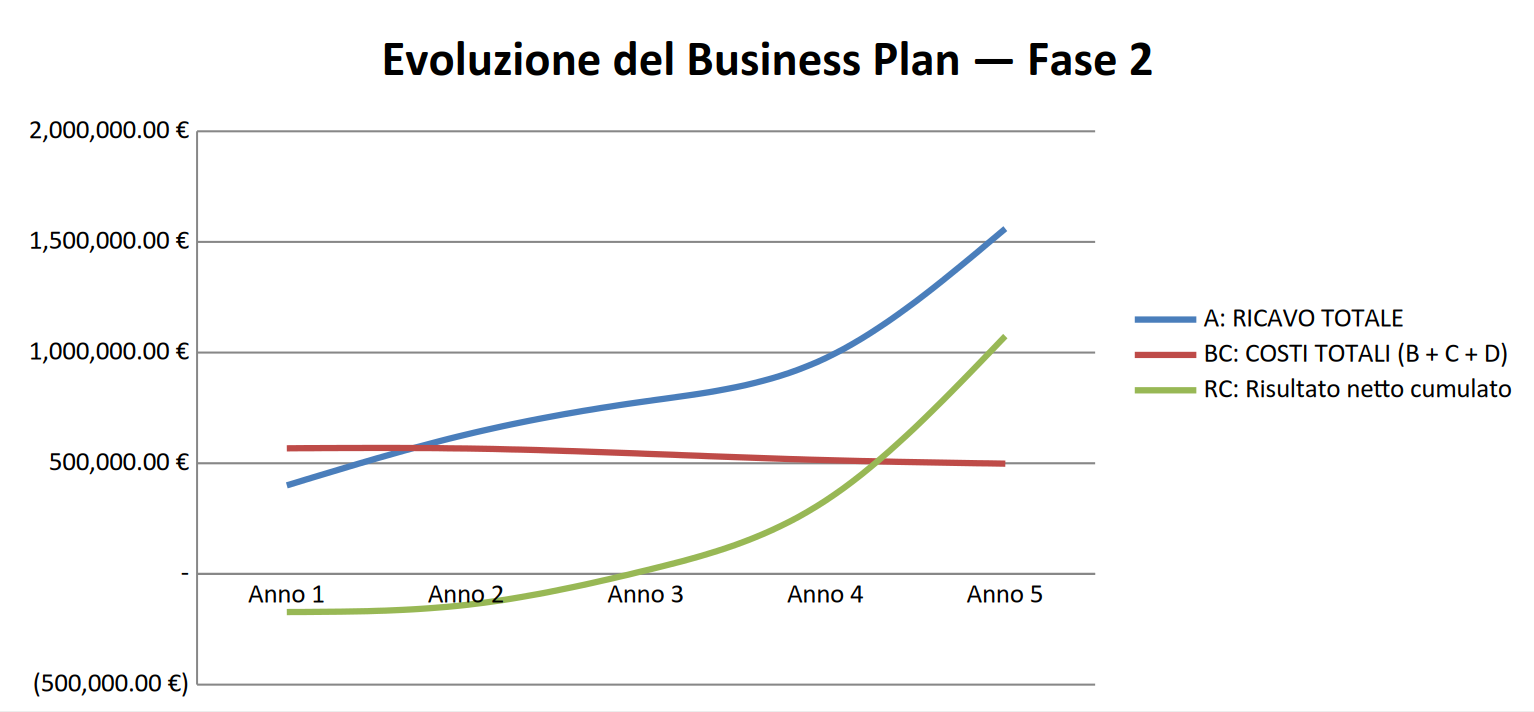
\includegraphics[width=\textwidth]{imgs/evoluzione.png}
    \caption{Evoluzione del Business Plan --- grafico di ricavi, costi e risultato netto cumulato nei cinque anni}
    \label{fig:evoluzione}
\end{figure}

Attraverso l'analisi dei dati previsionali \`e possibile determinare il \textbf{Break Even Point} (BEP). Il punto di pareggio individua il momento in cui il risultato netto cumulato dell'esercizio azzera l'investimento iniziale sostenuto nell'Anno~Zero: fino a quel momento l'iniziativa sta ancora recuperando il capitale impiegato, da quel momento in avanti inizia ad accumulare utile. Osservando la curva del \textit{Risultato Netto Cumulato} in Figura~\ref{fig:evoluzione}, si rileva che essa interseca l'asse dello zero in corrispondenza del \textbf{terzo anno} di esercizio, quando il risultato cumulato passa da $-139.867$ \euro{} a $+16.174$ \euro{}: da quel momento in avanti l'iniziativa economica inizia a generare un utile reale.

Un secondo indicatore fondamentale per valutare la sostenibilit\`a del progetto \`e il \textbf{ROI} (\textit{Return on Investment}), indice finanziario che misura la redditivit\`a del capitale investito esprimendo il guadagno generato per ogni euro allocato nella piattaforma:

\begin{equation}
    ROI = \frac{\text{Utile Netto}}{\text{Capitale Investito}} \times 100
\end{equation}

Coerentemente con la convenzione adottata, il \textbf{rendimento medio annuo} \`e ricavato dal
ROI sottraendo la quota del 100\% corrispondente alla restituzione del capitale investito e
ripartendo il residuo sui cinque anni di esercizio, in modo da esprimere il guadagno netto
prodotto mediamente in ciascuna annualit\`a per ogni euro allocato nella piattaforma.

\begin{table}[H]
\centering
\begin{tabular}{lr}
\hline
Risultato netto cumulato & 1.074.425,25 \\
Capitale investito       &   671.092,86 \\
\hline
\textbf{ROI in 5 anni}   & \textbf{160,10\%} \\
Rendimento annuo: (ROI $-$ 100\%) / 5 & 12,02\% \\
\hline
\end{tabular}
\caption{Indicatori di redditivit\`a del progetto}
\label{tab:roi}
\end{table}

I risultati ottenuti confermano la sostenibilit\`a economico-finanziaria dell'iniziativa (Tabella~\ref{tab:roi}). La piattaforma \`e in grado di assorbire l'investimento iniziale di 671.092,86 \euro{} e i costi ricorrenti di esercizio, raggiungendo il punto di pareggio nel corso del terzo anno di attivit\`a e generando, al termine del quinquennio, un risultato netto cumulato di circa 1,07 milioni di euro, con un rendimento medio annuo del 12,02\%.

\`E opportuno osservare che il pareggio viene raggiunto con un margine contenuto: il risultato cumulato del terzo anno si attesta a poco pi\`u di 16.000 \euro{}, valore che rende il conseguimento del BEP entro tale termine sensibile a scostamenti anche modesti nel ritmo di acquisizione dei clienti.

\`E opportuno inoltre osservare che il modello adottato si fonda su un'ipotesi di crescita graduale e prudente del portafoglio clienti e che non contabilizza alcuni dei flussi di ricavo previsti dal Business Model Canvas, quali l'addebito proporzionale al volume di DMVP registrati e il marketplace di servizi aggiuntivi. Il profilo di redditivit\`a rappresentato pu\`o pertanto essere considerato conservativo. Il principale fattore di rischio economico resta legato al ritmo di adesione degli intermediari alla piattaforma: un rallentamento nell'acquisizione dei primi clienti comporterebbe un incremento degli oneri su disavanzo operativo e un conseguente slittamento del Break Even Point, coerentemente con quanto evidenziato nell'analisi SWOT in merito alla necessit\`a di raggiungere una massa critica di attori nella filiera.
\chapter{Conclusioni}

Il presente documento ha esaminato la fattibilità e la progettazione di \textit{Tuning Ledger}, una piattaforma basata su tecnologia blockchain per la registrazione e la certificazione delle modifiche apportate ai veicoli dopo l'immatricolazione, con l'obiettivo di garantire trasparenza, autenticit\`a e verificabilit\`a delle informazioni lungo l'intero ciclo di vita del mezzo.

Lo studio ha preso avvio da un'analisi del contesto che ha messo in luce come la filiera dell'automotive tuning, pur avendo acquisito una rilevanza economica crescente, continui a fondarsi su strumenti documentali eterogenei e privi di garanzie di integrit\`a. La modellazione GOREM del contesto ha permesso di formalizzare gli obiettivi non funzionali dei soggetti coinvolti e le relazioni che intercorrono tra di essi, evidenziando come le qualit\`a attese dai diversi stakeholder siano in larga misura convergenti: un registro condiviso e non alterabile produce benefici simultanei lungo tutta la catena del valore. La medesima analisi ha per\`o portato alla luce il principale \textit{trade-off} progettuale del sistema, ossia la tensione tra l'apertura informativa richiesta dalla trasparenza e la tutela della riservatezza dei dati del proprietario, che ha trovato risposta nella definizione di politiche di accesso selettivo differenziate per ruolo.

La restrizione allo scenario specifico ha quindi consentito di definire il \textbf{Digital Modified Vehicle Passport} (DMVP) quale passaporto digitale immutabile associato al numero di telaio, e di individuare nell'\textbf{Intermediario} il cliente primario della piattaforma, attorno al quale \`e stato costruito il modello di business in Canvas. Sul piano tecnologico, il confronto con le soluzioni gi\`a disponibili sul mercato ha motivato l'adozione di una \textbf{blockchain permissioned} in \textbf{architettura ibrida}, nella quale i dati descrittivi e la documentazione risiedono \textit{off-chain} mentre sul registro distribuito viene ancorata la sola impronta crittografica: una scelta che preserva l'integrit\`a del dato contenendo al contempo costi operativi e limiti di scalabilit\`a.

I flussi informativi e le interazioni del sistema sono stati mappati in dettaglio attraverso i casi d'uso modellati in GOREM e i processi rappresentati in notazione BPMN, che hanno reso esplicite le responsabilit\`a dei singoli attori e la separazione tra componente applicativa e infrastruttura blockchain. L'analisi SWOT ha successivamente confermato la solidit\`a complessiva della proposta, individuandone i punti di forza nell'immutabilit\`a del passaporto, nell'efficienza dell'architettura ibrida e nella tutela legale offerta a tutti gli attori coinvolti, e riconducendo i principali fattori di rischio alla necessit\`a di raggiungere una massa critica di aderenti e di ottenere un riconoscimento istituzionale del DMVP.

Dal punto di vista realizzativo, il Project Plan ha delineato un percorso di \textbf{sei anni}, articolato in un anno di sviluppo e cinque di esercizio, con un impegno complessivo di \textbf{46,75 Anni-Persona} e un organico che passa dalle dodici unit\`a della fase di sviluppo alle otto della fase di esercizio, sostenuto da un'architettura a micro-servizi organizzata in cinque sottosistemi applicativi.

Sul piano economico-finanziario, il Business Plan ha validato la sostenibilit\`a dell'iniziativa. A fronte di un capitale investito di \textbf{671.092,86~\euro{}}, la piattaforma raggiunge il \textbf{Break Even Point nel corso del terzo anno} di esercizio e produce, al termine del quinquennio, un risultato netto cumulato di circa \textbf{1,07 milioni di euro}, corrispondente a un \textbf{ROI del 160,10\%} e a un rendimento medio annuo del \textbf{12,02\%}. Va peraltro osservato che la proiezione adottata \`e deliberatamente prudenziale: essa assume una crescita graduale del portafoglio clienti e non contabilizza alcuni dei flussi di ricavo previsti dal Business Model Canvas, tra cui l'addebito proporzionale al volume di DMVP registrati e il marketplace di servizi aggiuntivi. Il margine con cui il pareggio viene conseguito resta tuttavia contenuto, circostanza che rende il rispetto di tale traguardo sensibile al ritmo effettivo di adesione degli intermediari.

\section*{Vantaggi strategici}

Il lavoro svolto ha messo in evidenza i seguenti benefici derivanti dall'implementazione della piattaforma:

\begin{itemize}
    \item \textbf{Certezza e non alterabilit\`a delle informazioni}: l'ancoraggio degli \textit{hash} sul registro distribuito rende tecnicamente impossibile retrodatare un intervento, sostituire documentazione tecnica o dichiarare modifiche mai eseguite, trasformando la documentazione da insieme di atti sparsi in storico certificato del veicolo.

    \item \textbf{Tutela legale degli operatori}: la registrazione immutabile delle lavorazioni costituisce una prova documentale a favore dell'Azienda di Tuning contro contestazioni infondate e riduce l'esposizione della Concessionaria nella commercializzazione di veicoli modificati.

    \item \textbf{Efficienza dei processi di verifica}: la disponibilit\`a di dati gi\`a strutturati e verificabili abbrevia i tempi di collaudo del Centro di Certificazione e semplifica i controlli degli enti preposti, che possono accertare la conformit\`a del mezzo senza ricostruirne manualmente la storia.

    \item \textbf{Valorizzazione del veicolo}: la disponibilit\`a di uno storico certificato e trasferibile contrasta la svalutazione che oggi colpisce i mezzi modificati sul mercato dell'usato, poich\'e consente al proprietario di dimostrare la regolarit\`a e la qualit\`a delle personalizzazioni.

    \item \textbf{Sostenibilit\`a economica della soluzione tecnica}: l'architettura ibrida coniuga le garanzie di integrit\`a proprie della blockchain con l'efficienza dell'archiviazione tradizionale, rendendo economicamente praticabile un'adozione su scala industriale.
\end{itemize}

\section*{Sviluppi futuri}

Al di l\`a del perimetro dello scenario analizzato, la piattaforma offre alcune prospettive di evoluzione che meritano di essere segnalate:

\begin{itemize}
    \item \textbf{Estensione a segmenti contigui}: il modello del passaporto digitale pu\`o essere applicato al \textit{retrofit} elettrico, al restauro e alla certificazione dei veicoli storici, all'allestimento di veicoli commerciali e alla gestione documentale delle flotte aziendali, ambiti nei quali la tracciabilit\`a degli interventi riveste la medesima criticit\`a e che permetterebbero di ampliare in modo significativo il bacino d'utenza.

    \item \textbf{Riconoscimento istituzionale del DMVP}: l'attribuzione di un valore formale al passaporto digitale da parte della Motorizzazione Civile e del comparto assicurativo rappresenta la principale leva di diffusione della piattaforma, in quanto ne trasformerebbe la natura da adempimento aggiuntivo a strumento sostitutivo della documentazione tradizionale.

    \item \textbf{Integrazione con sistemi di intelligenza artificiale}: l'analisi dei dati storici raccolti sulla piattaforma consentirebbe di individuare correlazioni tra tipologie di modifica, componenti impiegati ed esiti dei collaudi, fornendo agli operatori indicazioni predittive sulla conformit\`a degli interventi in fase di progettazione.

    \item \textbf{Interoperabilit\`a con i passaporti digitali di prodotto}: la progressiva affermazione, a livello europeo, dei \textit{Digital Product Passport} apre alla possibilit\`a di allineare il DMVP a standard condivisi, favorendone il riconoscimento transfrontaliero e l'integrazione con i registri della componentistica.

    \item \textbf{Automazione contrattuale tramite smart contract}: l'estensione della logica \textit{on-chain} alla gestione delle garanzie e dei rapporti tra officine, fornitori e compagnie assicurative permetterebbe di automatizzare la verifica delle condizioni contrattuali sulla base di dati temporali non manipolabili.
\end{itemize}

In conclusione, lo studio conferma che \textit{Tuning Ledger} costituisce un'opportunit\`a concreta di innovazione per il settore della personalizzazione dei veicoli. La sua realizzazione non si limiterebbe a digitalizzare una documentazione oggi frammentaria, ma introdurrebbe uno strato di certificazione condiviso in grado di ridurre l'asimmetria informativa che caratterizza il mercato post-vendita, restituendo valore tanto agli operatori professionali quanto ai proprietari dei veicoli. La condizione di successo dell'iniziativa non risiede pertanto nella sola solidit\`a tecnica della soluzione, gi\`a verificata nel corso del presente lavoro, quanto piuttosto nella capacit\`a di aggregare attorno al registro un numero sufficiente di attori della filiera e di ottenere, dagli enti competenti, il riconoscimento che ne consacri il valore probatorio.

\begin{thebibliography}{9}

\bibitem{hyperledger}
E.~Androulaki, A.~Barger, V.~Bortnikov, C.~Cachin, K.~Christidis, A.~De~Caro,
D.~Enyeart, C.~Ferris, G.~Laventman, Y.~Manevich, S.~Muralidharan, C.~Murthy,
B.~Nguyen, M.~Sethi, G.~Singh, K.~Smith, A.~Sorniotti, C.~Stathakopoulou,
M.~Vukoli\'c, S.~Weed~Cocco, J.~Yellick,
\textit{Hyperledger Fabric: A Distributed Operating System for Permissioned
Blockchains}, in Proceedings of the Thirteenth EuroSys Conference (EuroSys~'18),
Porto, Portogallo, 23--26 aprile 2018, pp.~30:1--30:15.
\newblock DOI: \texttt{10.1145/3190508.3190538}.

\bibitem{murta2024}
J.~Murta, V.~Amaral, F.~Brito~e~Abreu,
\textit{Preserving Automotive Heritage: A Blockchain-Based Solution for Secure
Documentation of Classic Cars Restoration}, arXiv preprint
\texttt{arXiv:2403.08093} [cs.CY], marzo 2024, 20~pp.

\bibitem{nftvehicle}
J.~C.~L\'opez-Pimentel, L.~A.~Morales-Rosales, I.~Algredo-Badillo,
C.~Del-Valle-Soto,
\textit{NFT-Vehicle: A Blockchain-Based Tokenization Architecture to Register
Transactions over a Vehicle's Life Cycle}, Mathematics, vol.~11, n.~13, 2023,
art.~2801.
\newblock DOI: \texttt{10.3390/math11132801}.

\bibitem{espr}
Parlamento Europeo e Consiglio dell'Unione Europea,
\textit{Regolamento (UE) 2024/1781 del 13 giugno 2024 che istituisce un quadro
per l'elaborazione di specifiche di progettazione ecocompatibile per prodotti
sostenibili} (ESPR), Gazzetta Ufficiale dell'Unione Europea, 28 giugno 2024.
\newblock Il Capo~III istituisce il passaporto digitale del prodotto
(\textit{Digital Product Passport}).

\bibitem{cds}
Repubblica Italiana,
\textit{Decreto Legislativo 30 aprile 1992, n.~285 --- Nuovo codice della
strada}, art.~78, \textit{Modifiche delle caratteristiche costruttive dei
veicoli in circolazione e aggiornamento della carta di circolazione}.

\bibitem{dpr495}
Repubblica Italiana,
\textit{Decreto del Presidente della Repubblica 16 dicembre 1992, n.~495 ---
Regolamento di esecuzione e di attuazione del nuovo codice della strada},
art.~236, recante la disciplina attuativa dell'art.~78 del codice della strada.

\end{thebibliography}

\end{document}
